\documentclass[letterpaper,10pt]{book}
% Change to 10 pt
\usepackage{pdfpages}
\usepackage{morewrites}			% to counteract the no write space problem
\setcounter{tocdepth}{6}

\usepackage[framemethod=TikZ]{mdframed}

\usepackage{fancyhdr}

\usepackage{paralist}
\usepackage{amsmath}
\usepackage{amsfonts}
\usepackage{amssymb}
\usepackage{graphicx}

\usepackage{datetime}
%\usepackage{ulem}

%\usepackage[nottoc]{toobibind}

\usepackage[inline]{enumitem}

% Outer margin at 2.50 is exacty correct to fit the ``corruption alert'' tables
\usepackage[inner=1.0in, outer=2.50in, top=2.54cm,bottom=2.54cm, marginparwidth=2.25in]{geometry}

\usepackage{marginnote}
\usepackage{longtable}
\usepackage{booktabs}
\usepackage{xcolor}

\usepackage{soul}

%%%%%%%%%%%%
\definecolor{ForestGreen}{rgb}{0.00,0.29,0.098}
%%%%%%%%%%%%

\usepackage{marginnote}

\usepackage{imakeidx} 
\usepackage[
	backref=true,
	style=numeric,
%	citestyle=numeric,
	backend=bibtex
	]{biblatex}
\usepackage[driverfallback=hypertex,colorlinks=True]{hyperref}
\usepackage{cleveref}

\makeindex[name=scripture,columnsep=20pt, columnseprule=True,columns=3, title=Scripture References]
\makeindex[name=speaker,columnsep=20pt, columnseprule=True,,columns=2, title=Sermon Creator]
\makeindex[name=series,columnsep=20pt, columnseprule=True,,columns=2, title=Sermon Series]
\makeindex[name=date,columnsep=20pt, columnseprule=True,columns=2, title=Sermon Date]
\makeindex[name=event,columnsep=20pt, columnseprule=True,columns=2, title=Event]
\makeindex[name=topic,columnsep=20pt, columnseprule=True,columns=2, title=Topic]
\makeindex[name=AWIP,columnsep=20pt, columnseprule=True,columns=3, title=All Words in Passage]
\makeindex[name=NWIV,columnsep=20pt, columnseprule=True,columns=3, title=Number of Words in Verse]
\makeindex[name=PNIP,columnsep=20pt, columnseprule=True,columns=3, title=Proper Names in Passage]
\makeindex[name=PEIP,columnsep=20pt, columnseprule=True,columns=2, title=Prophetic Events in Passage]
\makeindex[name=TWPAQ,columnsep=20pt, columnseprule=True,columns=1, title=13-Word Phrases and Quotes]
\makeindex[name=PFTTIS,columnsep=20pt, columnseprule=False,columns=3, title=Phrases found 13 times in scripture]
\makeindex[name=WFTTIS,columnsep=20pt, columnseprule=False,columns=3, title=Words found 13 times in scripture]
\makeindex[name=WFITV,columnsep=20pt, columnseprule=False,columns=3, title=Words found in exactly 13 verses]
\makeindex[name=EVENTS,columnsep=20pt, columnseprule=False,columns=2, title=Sermon Log by Place]
\makeindex[name=QUESTIONS,columnsep=20pt, columnseprule=False,columns=2, title=Bible Questions]
\makeindex[name=DOCTRINES,columnsep=20pt, columnseprule=False,columns=2, title=Doctrines]
\makeindex[name=SONGS,columnsep=20pt, columnseprule=False,columns=1, title=Songs]
\makeindex[name=LOCATION,columnsep=20pt, columnseprule=False,columns= 2, title=Location]
\makeindex[name=FACEBOOK,columnsep=20pt, columnseprule=False,columns=2, title=Facebook]
\makeindex[name=DEVOTIONAL,columnsep=20pt, columnseprule=False,columns=2, title=Devotional Items]
%%%%%%%%%%%%%%%%% EXTRA COLORS
\definecolor{champagne}{rgb}{0.97,0.91,0.81}
\definecolor{bone}{rgb}{0.89,0.85,0.79}
\pagestyle{fancy}
\fancyhf{}
\fancyhead[LE,RO]{\today}
\fancyhead[RE,LO]{Daily Bible Reading}
\fancyhead[CE,CO]{-page \thepage  - }

\fancyfoot[CO,CE]{\leftmark}
%\fancyfoot[LE,RO]{CSCE 692, HW1}

\title{DBR\\
Daily \\ Reads}
\author{Keith Anthony \\
\today }
%+/ffffff +   \pagenumbering{gobble}
\bibliography{Bibliographies/All20220122}

\setlength{\fboxsep}{1.0pt}

\usepackage[utf8]{inputenc}
\usepackage{tikz}

\begin{document}
%%%%%%%%%%%% Tile Page

\begin{titlepage}

\begin{flushright}
\rightskip=-2.5cm
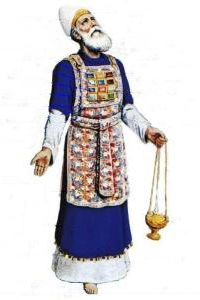
\includegraphics[width=50mm,scale=1.5]{Extras/Melchisedec.jpg}
\vspace{0.4in}  % Create a title for the document and write it in bold font
\LARGE{\textbf{\date}} % Again, do a line break
\linebreak 
% Create a subtitle \large{with Outlines, Statistics, Cross References, and Notes}
\vspace{0.5in}
\begin{flushleft}
\LARGE{Day \#70: Friday, 11 March 2022  \\}\vspace{0.25in}
\LARGE{Joshua 16-18 Psalm 70 Proverb 11}
\end{flushleft}
\vspace{0.6in}
\bigskip

\normalsize{Xenia, Oh.\\}
\normalsize{created: \today}
\vspace{1.3in}

\end{flushright}
\end{titlepage}

\newpage 
\tableofcontents\hypertarget{TOC}{}
\listoffigures
\listoftables

\hyphenation{A-bim-e-lech bre-thren E-phra-im  Gib-e-o-nites Jer-u-sa-lem through-out Phil-i-stines The-o-phil-us Am-a-le-kites ven-geance Mesh-el-e-mi-ah onan-ism Phar-a-oh thoughts grev-ous-ness Hach-a-liah adul-ter-er Shad-rach}

%%%%%%%%%%%%%%%%% EXTRA COLORS
%%%%%%%%%%%%%%%%% EXTRA COLORS
%%%%%%%%%%%%%%%%% EXTRA COLORS
\definecolor{champagne}{rgb}{0.97,0.91,0.81}
\definecolor{bone}{rgb}{0.89,0.85,0.79}

\definecolor{ForestGreen}{rgb}{0.00,0.29,0.098}
\definecolor{GIVING}{cmyk}{1,0.0,0.72,.1}

\definecolor{MLPE}{cmyk}{1,1,0,.45}
\definecolor{SOCCER}{cmyk}{.77, 0, .42, .49}
\definecolor{PAYBILL}{cmyk}{0,0.83,0.76,0.07}
\definecolor{SERMON}{cmyk}{.14,.9,0,.30} % aka seance \href{http://www.flatuicolorpicker.com/purple-cmyk-color-model/}{seance}
\definecolor{BIBLE}{cmyk}{0,.17,.74,.17}
\definecolor{WORKBLUE}{cmyk}{1, .5, 0, .6}
\definecolor{myOrange}{cmyk}{0, .4, .98, .03}
\definecolor{myTan}{cmyk}{0.0,.07,.17,.10}
\definecolor{myRed}{cmyk}{0,1,1,0}
\definecolor{myWhite}{cmyk}{0,0,0,0}
\definecolor{BLUESoD}{cmyk}{.97,.84,0,.04}
\definecolor{WHITE}{cmyk}{0,0,0,0}
\definecolor{OLDGOLD}{cmyk}{0.05,0.3,1.00,0}
\definecolor{CASTLETON}{cmyk}{1,0,0.31,0.66}
\definecolor{cadmiumgreen}{rgb}{0.0, 0.42, 0.24}
\definecolor{jungle}{rgb}{0.203,0.4882,0.1718}
\definecolor{MYGOLD}{rgb}{1,.84,0}

\definecolor{MYLIGHTGRAY}{rgb}{.85,.85,.85}

\definecolor{codegreen}{rgb}{0,0.6,0}
\definecolor{codegray}{rgb}{0.5,0.5,0.5}
\definecolor{codepurple}{rgb}{0.58,0,0.82}
\definecolor{backcolour}{rgb}{0.95,0.95,0.92}


\mdfdefinestyle{MyFrame}{%
    linecolor=blue,
    outerlinewidth=2pt,
    roundcorner=5pt,
    innertopmargin=\baselineskip,
    innerbottommargin=\baselineskip,
    innerrightmargin=10pt,
    innerleftmargin=10pt,
    backgroundcolor=gray!25!white}


\mdfdefinestyle{MyFrame2}{%
    linecolor=black,
    outerlinewidth=2pt,
    roundcorner=5pt,
    innertopmargin=\baselineskip,
    innerbottommargin=\baselineskip,
    innerrightmargin=10pt,
    innerleftmargin=10pt,
    backgroundcolor=yellow!25!white}


%%%%%
%% for PFTTIS list
%%%%%

%%% And Joseph said unto
\index[PFTTIS]{And Joseph said unto!Genesis!Gen 40:008}
\index[PFTTIS]{And Joseph said unto!Genesis!Gen 40:012}
\index[PFTTIS]{And Joseph said unto!Genesis!Gen 41:025}
\index[PFTTIS]{And Joseph said unto!Genesis!Gen 42:014}
\index[PFTTIS]{And Joseph said unto!Genesis!Gen 42:018}
\index[PFTTIS]{And Joseph said unto!Genesis!Gen 44:015}
\index[PFTTIS]{And Joseph said unto!Genesis!Gen 45:003}
\index[PFTTIS]{And Joseph said unto!Genesis!Gen 45:004}
\index[PFTTIS]{And Joseph said unto!Genesis!Gen 46:031}
\index[PFTTIS]{And Joseph said unto!Genesis!Gen 48:009}
\index[PFTTIS]{And Joseph said unto!Genesis!Gen 48:018}
\index[PFTTIS]{And Joseph said unto!Genesis!Gen 50:019}
\index[PFTTIS]{And Joseph said unto!Genesis!Gen 50:024}


%%% a shadow
\index[PFTTIS]{a shadow!1Chronicles!1Chr 029:15}
\index[PFTTIS]{a shadow!Job!Job 008:09}
\index[PFTTIS]{a shadow!Job!Job 014:02}
\index[PFTTIS]{a shadow!Job!Job 017:07}
\index[PFTTIS]{a shadow!Psalm!Psa 102:011}
\index[PFTTIS]{a shadow!Psalm!Psa 144:004}
\index[PFTTIS]{a shadow!Ecclesiastes!Eccl 006:012}
\index[PFTTIS]{a shadow!Ecclesiastes!Eccl 008:013}
\index[PFTTIS]{a shadow!Isaiah!Isa 04:006}
\index[PFTTIS]{a shadow!Isaiah!Isa 25:004}
\index[PFTTIS]{a shadow!Jonah!Jnh 04:06}
\index[PFTTIS]{a shadow!Colossians!Col 02:017}
\index[PFTTIS]{a shadow!Hebews!Heb 10:001}

%%% blessed is the man
\index[PFTTIS]{blessed is the man!Psalm!Psa 001:001}
\index[PFTTIS]{blessed is the man!Psalm!Psa 032:002}
\index[PFTTIS]{blessed is the man!Psalm!Psa 034:008}
\index[PFTTIS]{blessed is the man!Psalm!Psa 065:004}
\index[PFTTIS]{blessed is the man!Psalm!Psa 084:005}
\index[PFTTIS]{blessed is the man!Psalm!Psa 084:012}
\index[PFTTIS]{blessed is the man!Psalm!Psa 094:012}
\index[PFTTIS]{blessed is the man!Psalm!Psa 112:001}
\index[PFTTIS]{blessed is the man!Proverbs!Pro 008:034}
\index[PFTTIS]{blessed is the man!Isaiah!Isa 056:002}
\index[PFTTIS]{blessed is the man!Jeremiah!Jer 017:007}
\index[PFTTIS]{blessed is the man!Romans!Rom 004:008}
\index[PFTTIS]{blessed is the man!James!Jam 001:012}


%%% carry them
\index[PFTTIS]{carry them!Leviticus!Lev 14:045}
\index[PFTTIS]{carry them!Numbers!Num 11:012}
\index[PFTTIS]{carry them!Joshua!Jsh 04:003}
\index[PFTTIS]{carry them!1Samuel!1Sam 20:040}
\index[PFTTIS]{carry them!1Kings!1Kng 08:046}
\index[PFTTIS]{carry them!2Chronicles!2Chr 06:036}
\index[PFTTIS]{carry them!Ezra!Ezra 05:015}
\index[PFTTIS]{carry them!Isaiah!Isa 40:011}
\index[PFTTIS]{carry them!Isaiah!Isa 41:016}
\index[PFTTIS]{carry them!Isaiah!Isa 57:013}
\index[PFTTIS]{carry them!Jeremiah!Jer 20:004}
\index[PFTTIS]{carry them!Jeremiah!Jer 20:005}
\index[PFTTIS]{carry them!Jeremiah!Jer 43:012}


\index[PFTTIS]{good tidings!2Samuel!2Sam 18:027}
\index[PFTTIS]{good tidings!1Kings!1Ki 01:042}
\index[PFTTIS]{good tidings!2Kings!2Ki 07:009 (2x)}
\index[PFTTIS]{good tidings!Isaiah!Isa 40:009 (2x)}
\index[PFTTIS]{good tidings!Isaiah!Isa 41:007}
\index[PFTTIS]{good tidings!Isaiah!Isa 52:007}
\index[PFTTIS]{good tidings!Isaiah!Isa 61:001}
\index[PFTTIS]{good tidings!Nahum!Nah 01:005}
\index[PFTTIS]{good tidings!Luke!Lk 02:010}
\index[PFTTIS]{good tidings!1Thessalonians!1Thess 03:006}


%%% dead body
\index[PFTTIS]{dead body!Leviticus!Lev 21:011}
\index[PFTTIS]{dead body!Numbers!Num 06:006}
\index[PFTTIS]{dead body!Numbers!Num 09:006}
\index[PFTTIS]{dead body!Numbers!Num 09:007}
\index[PFTTIS]{dead body!Numbers!Num 09:010}
\index[PFTTIS]{dead body!Numbers!Num 09:011}
\index[PFTTIS]{dead body!Numbers!Num 09:013}
\index[PFTTIS]{dead body!Numbers!Num 09:016}
\index[PFTTIS]{dead body!2Kings!2Ki 08:005}
\index[PFTTIS]{dead body!Isaiah!Isa 26:019}
\index[PFTTIS]{dead body!Jeremiah!Jer 26:023}
\index[PFTTIS]{dead body!Jeremiah!Jer 36:030}
\index[PFTTIS]{dead body!Haggai!Hag 02:013}

%%% great sea
\index[PFTTIS]{great sea!Numbers!Num 34:006}
\index[PFTTIS]{great sea!Numbers!Num 34:007}
\index[PFTTIS]{great sea!Joshua!Jos 01:004}
\index[PFTTIS]{great sea!Joshua!Jos 09:001}
\index[PFTTIS]{great sea!Joshua!Jos 15:012}
\index[PFTTIS]{great sea!Joshua!Jos 15:047}
\index[PFTTIS]{great sea!Joshua!Jos 23:004}
\index[PFTTIS]{great sea!Ezekiel!Eze 47:010}
\index[PFTTIS]{great sea!Ezekiel!Eze 47:015}
\index[PFTTIS]{great sea!Ezekiel!Eze 47:019}
\index[PFTTIS]{great sea!Ezekiel!Eze 47:020}
\index[PFTTIS]{great sea!Ezekiel!Eze 48:028}
\index[PFTTIS]{great sea!Daniel!Dan 07:002}


%%% have forsaken me
\index[PFTTIS]{have forsaken me!Judges!Jdg 10:013}
\index[PFTTIS]{have forsaken me!1Samuel!1Sam 08:008}
\index[PFTTIS]{have forsaken me!1Kings!1Ki 11:033}
\index[PFTTIS]{have forsaken me!2Kings!2Ki 22:017}
\index[PFTTIS]{have forsaken me!2Chronicles!2Chr 12:005}
\index[PFTTIS]{have forsaken me!2Chronicles!2Chr 34:025}
\index[PFTTIS]{have forsaken me!Jeremiah!Jer 01:016}
\index[PFTTIS]{have forsaken me!Jeremiah!Jer 02:013}
\index[PFTTIS]{have forsaken me!Jeremiah!Jer 05:007}
\index[PFTTIS]{have forsaken me!Jeremiah!Jer 05:019}
\index[PFTTIS]{have forsaken me!Jeremiah!Jer 16:011 (2x)}
\index[PFTTIS]{have forsaken me!Jeremiah!Jer 19:004}

%%% no king
\index[PFTTIS]{no king!Judges!Jdg 17:06}
\index[PFTTIS]{no king!Judges!Jdg 18:01}
\index[PFTTIS]{no king!Judges!Jdg 19:01}
\index[PFTTIS]{no king!Judges!Jdg 21:25}
\index[PFTTIS]{no king!1Kings!1Ki 22:47}
\index[PFTTIS]{no king!2Kings!2Ki 23:25}
\index[PFTTIS]{no king!Nehemiah!Neh 13:26}
\index[PFTTIS]{no king!Psalms!Psa 033:016}
\index[PFTTIS]{no king!Proverbs!Pro 30:27}
\index[PFTTIS]{no king!Daniel!Dan 02:10}
\index[PFTTIS]{no king!Hosea!Hos 10:03}
\index[PFTTIS]{no king!Micah!Mic 04:09}
\index[PFTTIS]{no king!John!Jhn 19:15}


%%% rebellious house
\index[PFTTIS]{rebellious house!Exodus!Exo 02:005}
\index[PFTTIS]{rebellious house!Exodus!Exo 02:006}
\index[PFTTIS]{rebellious house!Exodus!Exo 02:008}
\index[PFTTIS]{rebellious house!Exodus!Exo 03:009}
\index[PFTTIS]{rebellious house!Exodus!Exo 03:026}
\index[PFTTIS]{rebellious house!Exodus!Exo 03:027}
\index[PFTTIS]{rebellious house!Exodus!Exo 12:002 (2x)}
\index[PFTTIS]{rebellious house!Exodus!Exo 12:003}
\index[PFTTIS]{rebellious house!Exodus!Exo 12:009}
\index[PFTTIS]{rebellious house!Exodus!Exo 12:025}
\index[PFTTIS]{rebellious house!Exodus!Exo 17:012}
\index[PFTTIS]{rebellious house!Exodus!Exo 24:003}

%%% seek him
\index[PFTTIS]{seek him!Deuteronomy!Deu 04:029}\index[PFTTIS]{seek him!1Samuel!1Sam 23:025}
\index[PFTTIS]{seek him!1Chronicles!1Chr 28:009}
\index[PFTTIS]{seek him!2Chronicles!1Chr 15:002}
\index[PFTTIS]{seek him!Ezra!Ezr 08:022}
\index[PFTTIS]{seek him!Psalms!Psa 022:026}
\index[PFTTIS]{seek him!Psalms!Psa 024:006}
\index[PFTTIS]{seek him!Psalms!Psa 119:002}
\index[PFTTIS]{seek him!SoS!SoS 03:002}
\index[PFTTIS]{seek him!SoS!SoS 06:001}
\index[PFTTIS]{seek him!Hosea!Hos 07:010}
\index[PFTTIS]{seek him!Amos!Amo 05:008}
\index[PFTTIS]{seek him!Hebrews!Heb 11:0063}


%%% seek ye
\index[PFTTIS]{seek ye!Isaiah!Isa 34:016}
\index[PFTTIS]{seek ye!Isaiah!Isa 45:019}
\index[PFTTIS]{seek ye!Isaiah!Isa 55:006}
\index[PFTTIS]{seek ye!Amos!Amos 5:004}
\index[PFTTIS]{seek ye!John!John 1:38}
\index[PFTTIS]{seek ye!John!John 18:4}
\index[PFTTIS]{seek ye!John!John 18:7}
\index[PFTTIS]{seek ye!Matthew!Matt 6:33}
\index[PFTTIS]{seek ye!Numbers!Num 16:10}
\index[PFTTIS]{seek ye!Luke!Luke 12:31}
\index[PFTTIS]{seek ye!Luke!Luke 24:5}
\index[PFTTIS]{seek ye!Psalm!Psa 27:8}
\index[PFTTIS]{seek ye!Zephaniah!Zeph 2:3}

%%% the uncircumcised
\index[PFTTIS]{the uncircumcised!Genesis!Gen 17:014}
\index[PFTTIS]{the uncircumcised!Judges!Jdg 14:003}
\index[PFTTIS]{the uncircumcised!Judges!Jdg 15:018}
\index[PFTTIS]{the uncircumcised!2Samuel!2Sam 01:020}
\index[PFTTIS]{the uncircumcised!Isaiah!Isa 02:001}
\index[PFTTIS]{the uncircumcised!Jeremiah!Jer 09:025}
\index[PFTTIS]{the uncircumcised!Ezekiel!Eze 28:010}
\index[PFTTIS]{the uncircumcised!Ezekiel!Eze 31:018}
\index[PFTTIS]{the uncircumcised!Ezekiel!Eze 32:019}
\index[PFTTIS]{the uncircumcised!Ezekiel!Eze 32:027}
\index[PFTTIS]{the uncircumcised!Ezekiel!Eze 32:028}
\index[PFTTIS]{the uncircumcised!Ezekiel!Eze 32:029}
\index[PFTTIS]{the uncircumcised!Ezekiel!Eze 32:032}

%%% worship him
\index[PFTTIS]{worship him!Psalms!Psa 97:007}
\index[PFTTIS]{worship him!Zephaniah!Zeph 02:011}
\index[PFTTIS]{worship him!Matthew!Matt 02:002}
\index[PFTTIS]{worship him!Matthew!Matt 02:008}
\index[PFTTIS]{worship him!John!John 04:023}
\index[PFTTIS]{worship him!John!John 04:024 (2x)} 
\index[PFTTIS]{worship him!Acts!Acts 17:023}
\index[PFTTIS]{worship him!Hebrews!Heb 01:006}
\index[PFTTIS]{worship him!Revelation!Rev 04:010}
\index[PFTTIS]{worship him!Revelation!Rev 13:008}
\index[PFTTIS]{worship him!Revelation!Rev 14:007}
\index[PFTTIS]{worship him!Revelation!Rev 19:010}


%%%%%
%% for PFTTIS list
%%%%%

%%% afflictions
\index[WFTTIS]{afflictions!Psalms!Psa 34:019}
\index[WFTTIS]{afflictions!Psalms!Psa 132:001}
\index[WFTTIS]{afflictions!Acts!Acts 07:010}
\index[WFTTIS]{afflictions!Acts!Acts 20:023}
\index[WFTTIS]{afflictions!2Corinthians!2Cor 06:004}
\index[WFTTIS]{afflictions!Colossians!Col 01:024}
\index[WFTTIS]{afflictions!1Thessalonians!1Thess 03:003}
\index[WFTTIS]{afflictions!2Timothy!2Tim 01:008}
\index[WFTTIS]{afflictions!2Timothy!2Tim 03:011}
\index[WFTTIS]{afflictions!2Timothy!2Tim 04:005}
\index[WFTTIS]{afflictions!Hebrews!Heb 10:032}
\index[WFTTIS]{afflictions!Hebrews!Heb 10:033}
\index[WFTTIS]{afflictions!1Peter!1Pet 05:009}

%%% acsend
\index[WFTTIS]{acsend!Joshua!Jos 06:05}
\index[WFTTIS]{acsend!Psalm!Psa 024:003}
\index[WFTTIS]{acsend!Psalm!Psa 135:007}
\index[WFTTIS]{acsend!Psalm!Psa 139:008}
\index[WFTTIS]{acsend!Isaiah!Isa 14:013}
\index[WFTTIS]{acsend!Isaiah!Isa 14:014}
\index[WFTTIS]{acsend!Jeremiah!Jer 10:013}
\index[WFTTIS]{acsend!Jeremiah!Jer 51:016}
\index[WFTTIS]{acsend!Ezekiel!Eze 38:009}
\index[WFTTIS]{acsend!John!John 06:062}
\index[WFTTIS]{acsend!John!John 20:017}
\index[WFTTIS]{acsend!Romans!Rom 10:006}
\index[WFTTIS]{acsend!Revelation!Rev 17:008}

%%% Assyrian
\index[WFTTIS]{Assyrian!Isaiah!Isa 10:005}
\index[WFTTIS]{Assyrian!Isaiah!Isa 10:024}
\index[WFTTIS]{Assyrian!Isaiah!Isa 14:025}
\index[WFTTIS]{Assyrian!Isaiah!Isa 19:023}
\index[WFTTIS]{Assyrian!Isaiah!Isa 23:013}
\index[WFTTIS]{Assyrian!Isaiah!Isa 30:031}
\index[WFTTIS]{Assyrian!Isaiah!Isa 31:008}
\index[WFTTIS]{Assyrian!Isaiah!Isa 52:004}
\index[WFTTIS]{Assyrian!Ezekiel!Eze 31:003}
\index[WFTTIS]{Assyrian!Hosea!Hos 05:013}
\index[WFTTIS]{Assyrian!Hosea!Hos 11:005}
\index[WFTTIS]{Assyrian!Micah!Hos 05:005}
\index[WFTTIS]{Assyrian!Micah!Hos 05:006}

%%% blot
\index[WFTTIS]{blot!Exodus!Exo 32:032}
\index[WFTTIS]{blot!Exodus!Exo 32:033}
\index[WFTTIS]{blot!Numbers!Num 05:026}
\index[WFTTIS]{blot!Deuteronomy!Deut 09:014}
\index[WFTTIS]{blot!Deuteronomy!Deut 25:019}
\index[WFTTIS]{blot!Deuteronomy!Deut 29:020}
\index[WFTTIS]{blot!2Kings!2Ki 14:027}
\index[WFTTIS]{blot!Job!Job 31:007}
\index[WFTTIS]{blot!Psalms!Psa 51:001}
\index[WFTTIS]{blot!Psalms!Psa 51:009}
\index[WFTTIS]{blot!Proverbs!Pro 09:007}
\index[WFTTIS]{blot!Jeremiah!Jer 18:023}
\index[WFTTIS]{blot!Revelation!Rev 03:005}


%%% chain
\index[WFTTIS]{chain!Genesis!Gen 41:042}
\index[WFTTIS]{chain!1Kings!1Ki 07:017}
\index[WFTTIS]{chain!Psalms!Psa 73:006}
\index[WFTTIS]{chain!SoS!Sos 04:009}
\index[WFTTIS]{chain!Lamentations!Lam 03:007}
\index[WFTTIS]{chain!Ezekiel!Eze 07:023}
\index[WFTTIS]{chain!Ezekiel!Eze 16:011}
\index[WFTTIS]{chain!Daniel!Dan 05:007}
\index[WFTTIS]{chain!Daniel!Dan 05:016}
\index[WFTTIS]{chain!Daniel!Dan 05:029}
\index[WFTTIS]{chain!Acts!Acts 28:020}
\index[WFTTIS]{chain!2Timothy!2Tim 01:016}
\index[WFTTIS]{chain!Revelation!Rev 20:001}


%%% controversy
\index[WFTTIS]{controversy!Deuteronomy!Deu 17:008}
\index[WFTTIS]{controversy!Deuteronomy!Deu 19:017}
\index[WFTTIS]{controversy!Deuteronomy!Deu 21:005}
\index[WFTTIS]{controversy!Deuteronomy!Deu 25:001}
\index[WFTTIS]{controversy!2Samuel!2Sam 15:002}
\index[WFTTIS]{controversy!Isaiah!Isa 34:008}
\index[WFTTIS]{controversy!Jeremiah!Jer 25:031}
\index[WFTTIS]{controversy!Ezekiel!Eze 44:024}
\index[WFTTIS]{controversy!Hosea!Hos 04:001}
\index[WFTTIS]{controversy!Hosea!Hos 12:002}
\index[WFTTIS]{controversy!Micah!Mic 06:002 (2x)}
\index[WFTTIS]{controversy!1Timothy!1Tim 03:016}


%%% Dagon/Dagon's
\index[WFTTIS]{Dagon!Judges!Jdg 16:023}
\index[WFTTIS]{Dagon!1Samuel!1Sam 05:002 (2x)}
\index[WFTTIS]{Dagon!1Samuel!1Sam 05:003 (2x)}
\index[WFTTIS]{Dagon!1Samuel!1Sam 05:004 (3x)}
\index[WFTTIS]{Dagon!1Samuel!1Sam 05:005 (3x)}
\index[WFTTIS]{Dagon!1Samuel!1Sam 05:007}
\index[WFTTIS]{Dagon!1Chronicles!1Chr 10:010}

%%% disobedient
\index[WFTTIS]{disobedient!1Kings!1Ki 13:026}
\index[WFTTIS]{disobedient!Nehemiah!Neh 09:026}
\index[WFTTIS]{disobedient!Luke!Luke 01:017}
\index[WFTTIS]{disobedient!Acts!Acts 26:019}
\index[WFTTIS]{disobedient!Romans!Rom 01:030}
\index[WFTTIS]{disobedient!Romans!Rom 10:021}
\index[WFTTIS]{disobedient!1Timothy!1Tim 01:009}
\index[WFTTIS]{disobedient!2Timothy!2Tim 03:002}
\index[WFTTIS]{disobedient!Titus!Titus 01:016}
\index[WFTTIS]{disobedient!Titus!Titus 03:003}
\index[WFTTIS]{disobedient!1Peter!1Pet 02:007}
\index[WFTTIS]{disobedient!1Peter!1Pet 02:008}
\index[WFTTIS]{disobedient!1Peter!1Pet 03:020}


%%% doubt
\index[WFTTIS]{doubt!Genesis!Gen 37:033}
\index[WFTTIS]{doubt!Deuteronomy!Deu 28:066}
\index[WFTTIS]{doubt!Job!Job 12:002}
\index[WFTTIS]{doubt!Matthew!Matt 14:031}
\index[WFTTIS]{doubt!Matthew!Matt 21:021}
\index[WFTTIS]{doubt!Mark!Mk 11:023}
\index[WFTTIS]{doubt!Luke!Lk 11:020}
\index[WFTTIS]{doubt!John!Jhn 10:024}
\index[WFTTIS]{doubt!Acts!Acts 02:012}
\index[WFTTIS]{doubt!Acts!Acts 28:004}
\index[WFTTIS]{doubt!1Corinthians!1Cor 09:010}
\index[WFTTIS]{doubt!Galatians!Gal 04:020}
\index[WFTTIS]{doubt!1John!1Jhn 02:019}


%%% dungeon
\index[WFTTIS]{dungeon!Genesis!Gen 40:015}
\index[WFTTIS]{dungeon!Genesis!Gen 41:014}
\index[WFTTIS]{dungeon!Exodus!Exo 12:029}
\index[WFTTIS]{dungeon!Jeremiah!Jer 37:016}
\index[WFTTIS]{dungeon!Jeremiah!Jer 38:006 (2x)}
\index[WFTTIS]{dungeon!Jeremiah!Jer 38:007}
\index[WFTTIS]{dungeon!Jeremiah!Jer 38:009}
\index[WFTTIS]{dungeon!Jeremiah!Jer 38:010}
\index[WFTTIS]{dungeon!Jeremiah!Jer 38:011}
\index[WFTTIS]{dungeon!Jeremiah!Jer 38:013}
\index[WFTTIS]{dungeon!Lamentations!Lam 03:053}
\index[WFTTIS]{dungeon!Lamentations!Lam 03:055}


%%% error
\index[WFTTIS]{error!2Samuel!2Sam 06:007}
\index[WFTTIS]{error!Job!Job 19:004}
\index[WFTTIS]{error!Ecclesiastes!Ecc 05:006}
\index[WFTTIS]{error!Ecclesiastes!Ecc 10:005}
\index[WFTTIS]{error!Isaiah!Isa 32:006}
\index[WFTTIS]{error!Daniel!Dan 06:004}
\index[WFTTIS]{error!Matthew!Matt 27:064}
\index[WFTTIS]{error!Romans!Rom 01:027}
\index[WFTTIS]{error!James!Jam 05:020}
\index[WFTTIS]{error!2Peter!2Pet 02:018}
\index[WFTTIS]{error!2Peter!2Pet 03:017}
\index[WFTTIS]{error!1John!1Jn 04:006}
\index[WFTTIS]{error!Jude!Jude 01:011}

%%% fourish
\index[WFTTIS]{fourish!Psalms!Psa 072:007}
\index[WFTTIS]{fourish!Psalms!Psa 072:016}
\index[WFTTIS]{fourish!Psalms!Psa 092:007}
\index[WFTTIS]{fourish!Psalms!Psa 092:012}
\index[WFTTIS]{fourish!Psalms!Psa 092:013}
\index[WFTTIS]{fourish!Psalms!Psa 132:018}
\index[WFTTIS]{fourish!Proverbs!Pro 11:28}
\index[WFTTIS]{fourish!Proverbs!Pro 14:11}
\index[WFTTIS]{fourish!Ecclesiastes!Ecc 12:05}
\index[WFTTIS]{fourish!SongOfSolomon!SOS 07:12}
\index[WFTTIS]{fourish!Isaiah!Isa 17:11}
\index[WFTTIS]{fourish!Isaiah!Isa 66:14}
\index[WFTTIS]{fourish!Ezekiel!Eze 17:24}




%%% giants
\index[WFTTIS]{giants!Genesis!Gen 06:004}
\index[WFTTIS]{giants!Numbers!Num 13:033}
\index[WFTTIS]{giants!Deuteronomy!Deut 02:011}
\index[WFTTIS]{giants!Deuteronomy!Deut 02:021}
\index[WFTTIS]{giants!Deuteronomy!Deut 03:011}
\index[WFTTIS]{giants!Deuteronomy!Deut 03:013}
\index[WFTTIS]{giants!Joshua!Josh 12:004}
\index[WFTTIS]{giants!Joshua!Josh 13:012}
\index[WFTTIS]{giants!Joshua!Josh 15:008}
\index[WFTTIS]{giants!Joshua!Josh 17:015}
\index[WFTTIS]{giants!Joshua!Josh 16:016}

%%% good man
\index[WFTTIS]{good man!2 Samuel!2Sa 18:27}
%(1) Psalms 37:23 [5]
%(1) Psalms 112:5 [2]
%(1) Proverbs 12:2 [2]
%(1) Proverbs 13:22 [2]
%(1) Proverbs 14:14 [14]
%(1) Micah 7:2 [2]
%(1) Matthew 12:35 [2]
%(1) Luke 6:45 [2]
%(1) Luke 23:50 [15]
%(1) John 7:12 [17]
%(1) Acts 11:24 [5]
%(1) Romans 5:7 [14]

%%% Hinnom
\index[WFTTIS]{Hinnom!Joshua!Jsh 15:008}
\index[WFTTIS]{Hinnom!Joshua!Jsh 18:016}
\index[WFTTIS]{Hinnom!2Kings!2Ki 23:010}
\index[WFTTIS]{Hinnom!2Chronicles!2Chr 28:003}
\index[WFTTIS]{Hinnom!2Chronicles!2Chr 33:006}
\index[WFTTIS]{Hinnom!Nehemiah!Neh 11:030}
\index[WFTTIS]{Hinnom!Jeremiah!Jer 07:031}
\index[WFTTIS]{Hinnom!Jeremiah!Jer 07:032}
\index[WFTTIS]{Hinnom!Jeremiah!Jer 19:002}
\index[WFTTIS]{Hinnom!Jeremiah!Jer 19:006}
\index[WFTTIS]{Hinnom!Jeremiah!Jer 32:035}

%%% inclined
\index[WFTTIS]{inclined!Judges!Jdg 09:003}
\index[WFTTIS]{inclined!Psalms!Psa 040:001}
\index[WFTTIS]{inclined!Psalms!Psa 116:002}
\index[WFTTIS]{inclined!Psalms!Psa 119:112}
\index[WFTTIS]{inclined!Proverbs!Pro 05:13}
\index[WFTTIS]{inclined!Jeremiah!Jer 07:24}
\index[WFTTIS]{inclined!Jeremiah!Jer 07:26}
\index[WFTTIS]{inclined!Jeremiah!Jer 11:08}
\index[WFTTIS]{inclined!Jeremiah!Jer 17:23}
\index[WFTTIS]{inclined!Jeremiah!Jer 25:04}
\index[WFTTIS]{inclined!Jeremiah!Jer 34:14}
\index[WFTTIS]{inclined!Jeremiah!Jer 35:15}
\index[WFTTIS]{inclined!Jeremiah!Jer 44:05}


%%% laughed
\index[WFTTIS]{laughed!Genesis!Gen 17:017}
\index[WFTTIS]{laughed!Genesis!Gen 18:012}
\index[WFTTIS]{laughed!Genesis!Gen 18:015}
\index[WFTTIS]{laughed!2Kings!2Ki 19:021}
\index[WFTTIS]{laughed!2Chronicles!2Chr 30:010}
\index[WFTTIS]{laughed!Nehemiah!Neh 02:019}
\index[WFTTIS]{laughed!Job!Job 12:004}
\index[WFTTIS]{laughed!Job!Job 29:024}
\index[WFTTIS]{laughed!Isaiah!Isa 37:022}
\index[WFTTIS]{laughed!Ezekiel!Ezek 23:032}
\index[WFTTIS]{laughed!Matthew!Matt 09:024}
\index[WFTTIS]{laughed!Mark!Mk 05:040}
\index[WFTTIS]{laughed!Luke!Lk 08:053}

%%% liar
\index[WFTTIS]{liar!Job!Job 24:025}
\index[WFTTIS]{liar!Proverbs!Pro 17:004}
\index[WFTTIS]{liar!Proverbs!Pro 19:022}
\index[WFTTIS]{liar!Proverbs!Pro 30:006}
\index[WFTTIS]{liar!Jeremiah!Jer 15:018}
\index[WFTTIS]{liar!John!Jhn 08:044}
\index[WFTTIS]{liar!John!Jhn 08:055}
\index[WFTTIS]{liar!Romans!Rom 03:004}
\index[WFTTIS]{liar!1John!1Jhn 01:010}
\index[WFTTIS]{liar!1John!1Jhn 02:004}
\index[WFTTIS]{liar!1John!1Jhn 02:022}
\index[WFTTIS]{liar!1John!1Jhn 04:020}
\index[WFTTIS]{liar!1John!1Jhn 05:010}

%%% palsy
\index[WFTTIS]{palsy!Matthew!Matt 04:024}
\index[WFTTIS]{palsy!Matthew!Matt 08:006}
\index[WFTTIS]{palsy!Matthew!Matt 09:002}
\index[WFTTIS]{palsy!Matthew!Matt 09:006}
\index[WFTTIS]{palsy!Mark!Mk 02:003}
\index[WFTTIS]{palsy!Mark!Mk 02:004}
\index[WFTTIS]{palsy!Mark!Mk 02:005}
\index[WFTTIS]{palsy!Mark!Mk 02:009}
\index[WFTTIS]{palsy!Mark!Mk 02:010}
\index[WFTTIS]{palsy!Luke!Lk 05:018}
\index[WFTTIS]{palsy!Luke!Lk 05:024}
\index[WFTTIS]{palsy!Acts!Acts 09:033}

%%% Profitable
\index[WFTTIS]{profitable!Job!Job 22:002 (2x)}
\index[WFTTIS]{profitable!Ecclesiastes!Ecc 10:010}
\index[WFTTIS]{profitable!Isaiah!Isa 44:010}
\index[WFTTIS]{profitable!Jeremiah!Jer 13:007}
\index[WFTTIS]{profitable!Matthew!Matt 05:029}
\index[WFTTIS]{profitable!Matthew!Matt 05:030}
\index[WFTTIS]{profitable!Acts!Acts 20:020}
\index[WFTTIS]{profitable!1Timothy!1Tim 04:008}
\index[WFTTIS]{profitable!2Timothy!2Tim 03:016}
\index[WFTTIS]{profitable!2Timothy!2Tim 04:011}
\index[WFTTIS]{profitable!Titus!Titus 03:008}
\index[WFTTIS]{profitable!Philemon!Phlm 01:011}

%%% Rechab
\index[WFTTIS]{Rechab!2Samuel!2Sam 04:002}
\index[WFTTIS]{Rechab!2Samuel!2Sam 04:005}
\index[WFTTIS]{Rechab!2Samuel!2Sam 04:006}
\index[WFTTIS]{Rechab!2Samuel!2Sam 04:009}
\index[WFTTIS]{Rechab!2KIngs!2Ki 10:015}
\index[WFTTIS]{Rechab!2KIngs!2Ki 10:023}
\index[WFTTIS]{Rechab!1Chronicles!1Chr 02:055}
\index[WFTTIS]{Rechab!Nehemiah!Neh 03:014}
\index[WFTTIS]{Rechab!Jeremiah!Jer 35:006}
\index[WFTTIS]{Rechab!Jeremiah!Jer 35:008}
\index[WFTTIS]{Rechab!Jeremiah!Jer 35:014}
\index[WFTTIS]{Rechab!Jeremiah!Jer 35:016}
\index[WFTTIS]{Rechab!Jeremiah!Jer 35:019}

%%% serpents
\index[WFTTIS]{serpents!Exodus!Exo 07:012}
\index[WFTTIS]{serpents!Numbers!Num 21:006}
\index[WFTTIS]{serpents!Numbers!Num 21:007}
\index[WFTTIS]{serpents!Deuteronomy!Deu 08:015}
\index[WFTTIS]{serpents!Deuteronomy!Deu 32:024}
\index[WFTTIS]{serpents!Jeremiah!Jer 08:017}
\index[WFTTIS]{serpents!Matthew!Matt 10:016}
\index[WFTTIS]{serpents!Matthew!Matt 23:033}
\index[WFTTIS]{serpents!Mark!Mk 16:018}
\index[WFTTIS]{serpents!Luke!Lk 10:019}
\index[WFTTIS]{serpents!1Corinthians!1Cor 10:009}
\index[WFTTIS]{serpents!James!Jas 03:007}
\index[WFTTIS]{serpents!Revelation!Rev 09:019}

%%% short
\index[WFTTIS]{short!Numbers!Num 11:023}
\index[WFTTIS]{short!2Kings!2Ki 10:032}
\index[WFTTIS]{short!Job!Job 17:012}
\index[WFTTIS]{short!Job!Job 20:005}
\index[WFTTIS]{short!Psalms!Psa 89:047}
\index[WFTTIS]{short!Romans!Rom 03:023}
\index[WFTTIS]{short!Romans!Rom 09:028  (2x)}
\index[WFTTIS]{short!1Corinthians!1Cor 07:029}
\index[WFTTIS]{short!1Thessalonians!1Thess 02:017}
\index[WFTTIS]{short!Hebrews!Heb 04:001}
\index[WFTTIS]{short!Revelation!Rev 12:012}
\index[WFTTIS]{short!Revelation!Rev 17:010}

%%% smiteth
\index[WFTTIS]{smiteth!Exodus!Exo 21:012}
\index[WFTTIS]{smiteth!Exodus!Exo 21:15}
\index[WFTTIS]{smiteth!Deuteronomy!Dt 25:11}
\index[WFTTIS]{smiteth!Deuteronomy!Dt 27:24}
\index[WFTTIS]{smiteth!Joshua!Jsh 15:16}
\index[WFTTIS]{smiteth!Judges!Jdg 15:16}
\index[WFTTIS]{smiteth!2 Samuel!2Sa 05:08}
\index[WFTTIS]{smiteth!1Chronicles!1Chr 11:06}
\index[WFTTIS]{smiteth!Job!1Chr 26:12}
\index[WFTTIS]{smiteth!Isaiah!Isa 09:13}
\index[WFTTIS]{smiteth!Lamentations!Lam 03:30}
\index[WFTTIS]{smiteth!Ezekiel!Eze 07:09}
\index[WFTTIS]{smiteth!Luke!Lk 06:29}



%%% vanities
\index[WFTTIS]{vanities!Deuteronomy!Deut 21:021}
\index[WFTTIS]{vanities!1Kings!1Ki 16:013}
\index[WFTTIS]{vanities!1Kings!1Ki 16:026}
\index[WFTTIS]{vanities!Psalms!Psa 031:006}
\index[WFTTIS]{vanities!Ecclesiastes!Ecc 01:002 (2x)}
\index[WFTTIS]{vanities!Ecclesiastes!Ecc 05:007}
\index[WFTTIS]{vanities!Ecclesiastes!Ecc 12:008}
\index[WFTTIS]{vanities!Jeremiah!Jer 08:019}
\index[WFTTIS]{vanities!Jeremiah!Jer 10:008}
\index[WFTTIS]{vanities!Jeremiah!Jer 14:022}
\index[WFTTIS]{vanities!Jonah!Jnh 02:008}
\index[WFTTIS]{vanities!Acts!Acts 14:015}



%%%%%
%% for PFTTIS list
%%%%%

%%% worm
\index[WFITV]{worm!Exodus!Exo 16:024}
\index[WFITV]{worm!Job!Job 17:014}
\index[WFITV]{worm!Job!Job 24:029}
\index[WFITV]{worm!Job!Job 25:005 (2x)}
\index[WFITV]{worm!Psalms!Psa 022:006}
\index[WFITV]{worm!Isaiah!Isa 14:011}
\index[WFITV]{worm!Isaiah!Isa 41:014}
\index[WFITV]{worm!Isaiah!Isa 51:008}
\index[WFITV]{worm!Isaiah!Isa 66:024}
\index[WFITV]{worm!Jonah!Jnh 04:007}
\index[WFITV]{worm!Mark!Mk 09:044}
\index[WFITV]{worm!Mark!Mk 09:046}
\index[WFITV]{worm!Mark!Mk 09:048}


%\subsubsection{Title}
%\textbf{Introduction:} Isaiah 46 
%\index[speaker]{Speaker!Isaiah 49 (Title}
%\index[series]{Book (Speaker)!IPassage (Title)}
%\index[date]{2017/07/09!Isaiah 49 (Title)}
%\begin{compactenum}[I.]
%    \item  \textbf{Point} \index[scripture]{Isaiah!IPassage} (IPassage)
%\end{compactenum}




  


%\input{02OT-Exodus/ExodusIntroduction}

%\newpage
%\begin{figure}
%\begin{center}
%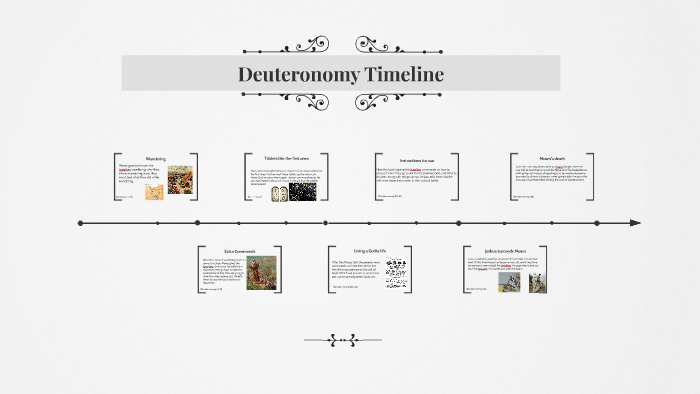
\includegraphics[scale=.7, angle=0]{05OT-Deuteronomy/References/AndrewSmithDeuteronomyTimeline.png}
%\caption[Deuteronomy Timeline by Andrew Smith]{Deuteronomy Timeline by Andrew %Smith}
%\label{fig:Deuteronomy Timeline by Andrew Smith}
%\end{center}
%\end{figure}

\newpage
\begin{figure}
\begin{center}
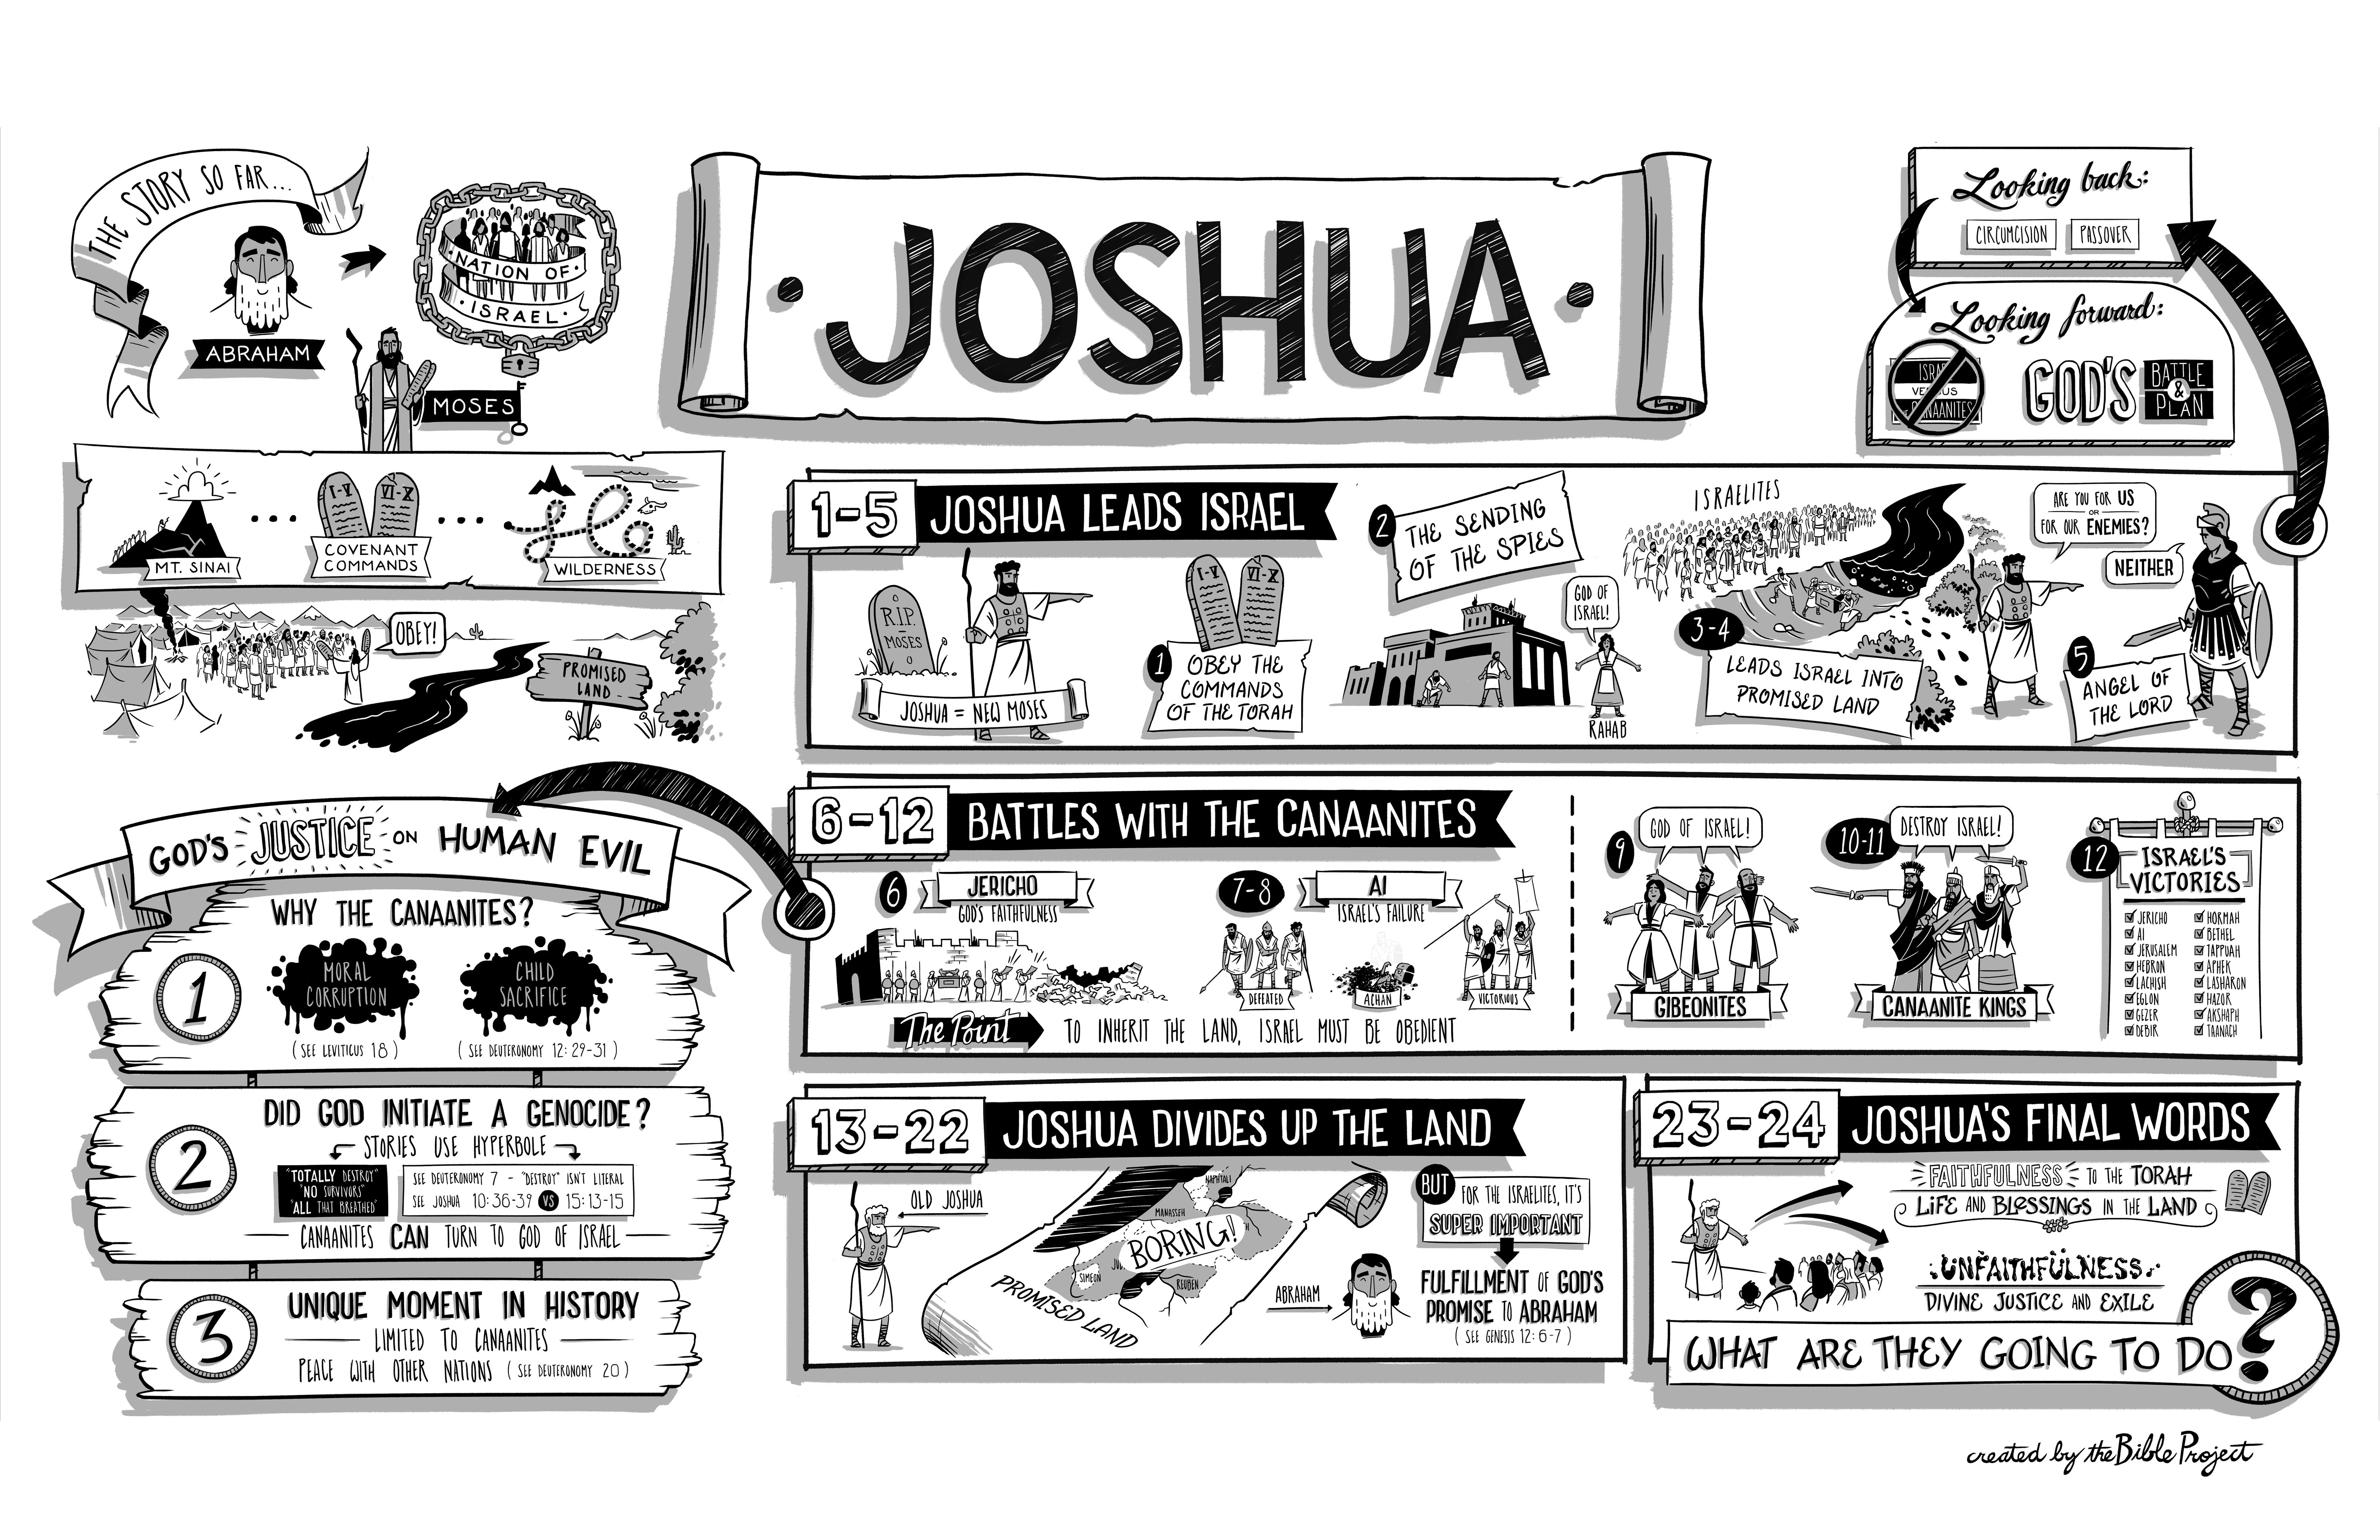
\includegraphics[scale=0.5, angle=90]{06OT-Joshua/References/1.BibleProject-Joshua.jpg}
\caption[Joshua from the Bible Project]{Joshua from the Bible Project}
\label{fig:Joshua from the Bible Project}
\end{center}
\end{figure}

\newpage
\begin{figure}
\begin{center}
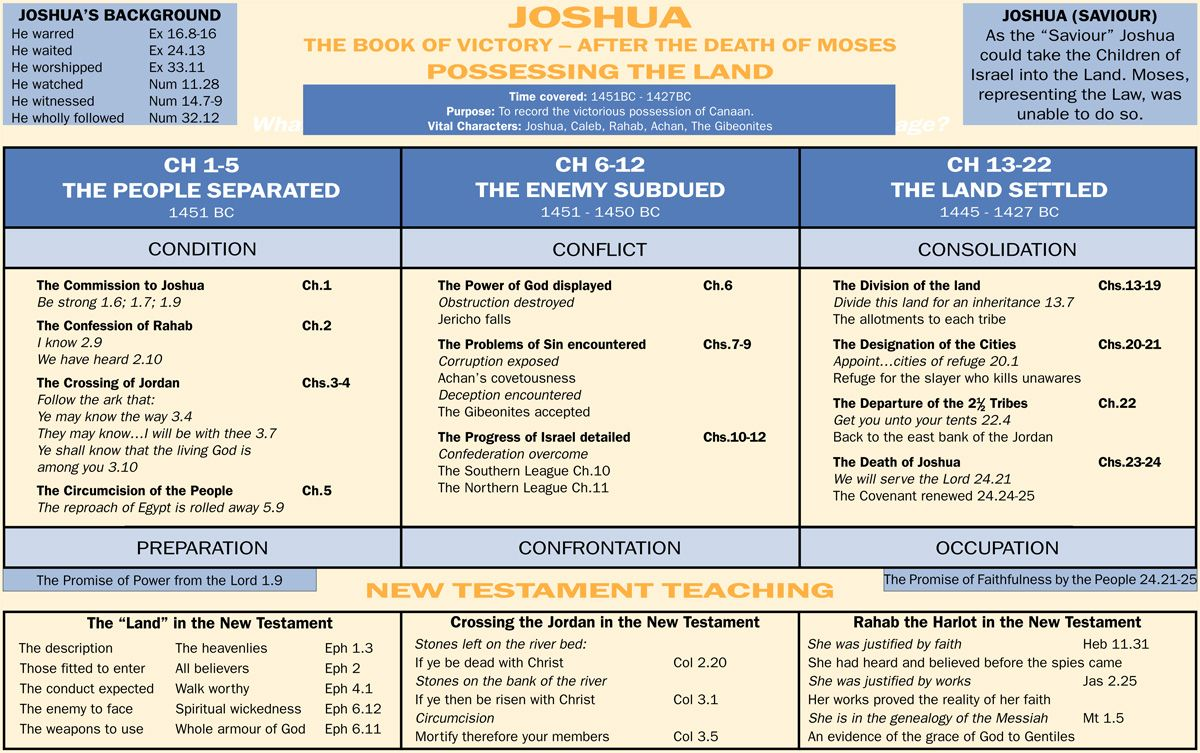
\includegraphics[scale=0.5, angle=90]{06OT-Joshua/References/2.JohnGrant-Joshua.jpg}
\caption[Joshua from John Grant]{Joshua from John Grant}
\label{fig:Joshua from John Grant}
\end{center}
\end{figure}

\newpage
\begin{figure}
\begin{center}
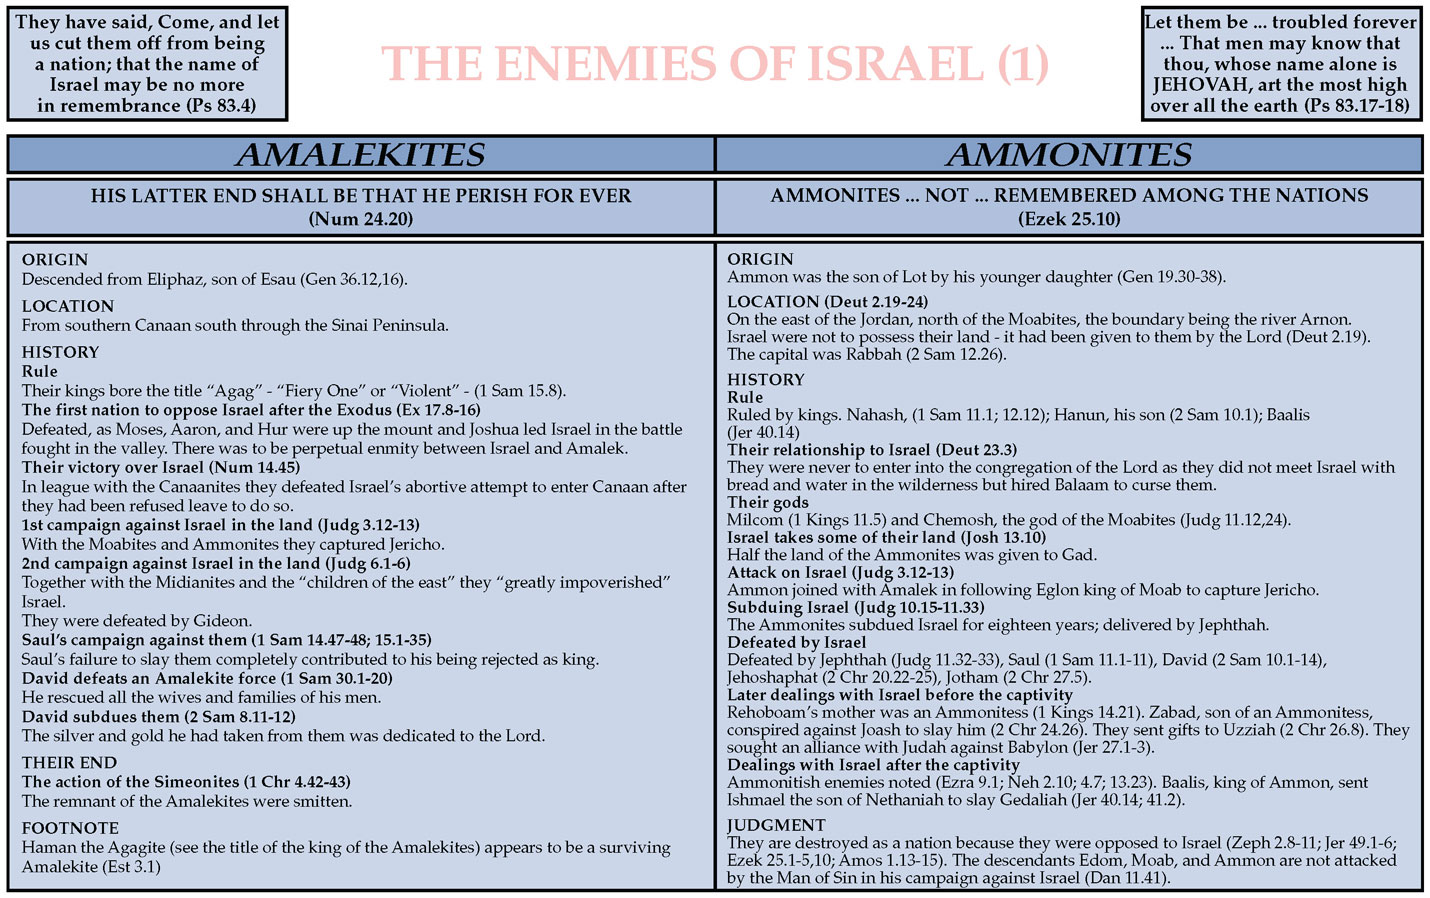
\includegraphics[scale=0.4, angle=90]{06OT-Joshua/References/3.EnemiesOfIsrael1.jpg}
\caption[Enemies of Israel 1]{Enemies of Israel 1}
\label{fig:Enemies of Israel 1}
\end{center}
\end{figure}

\newpage
\begin{figure}
\begin{center}
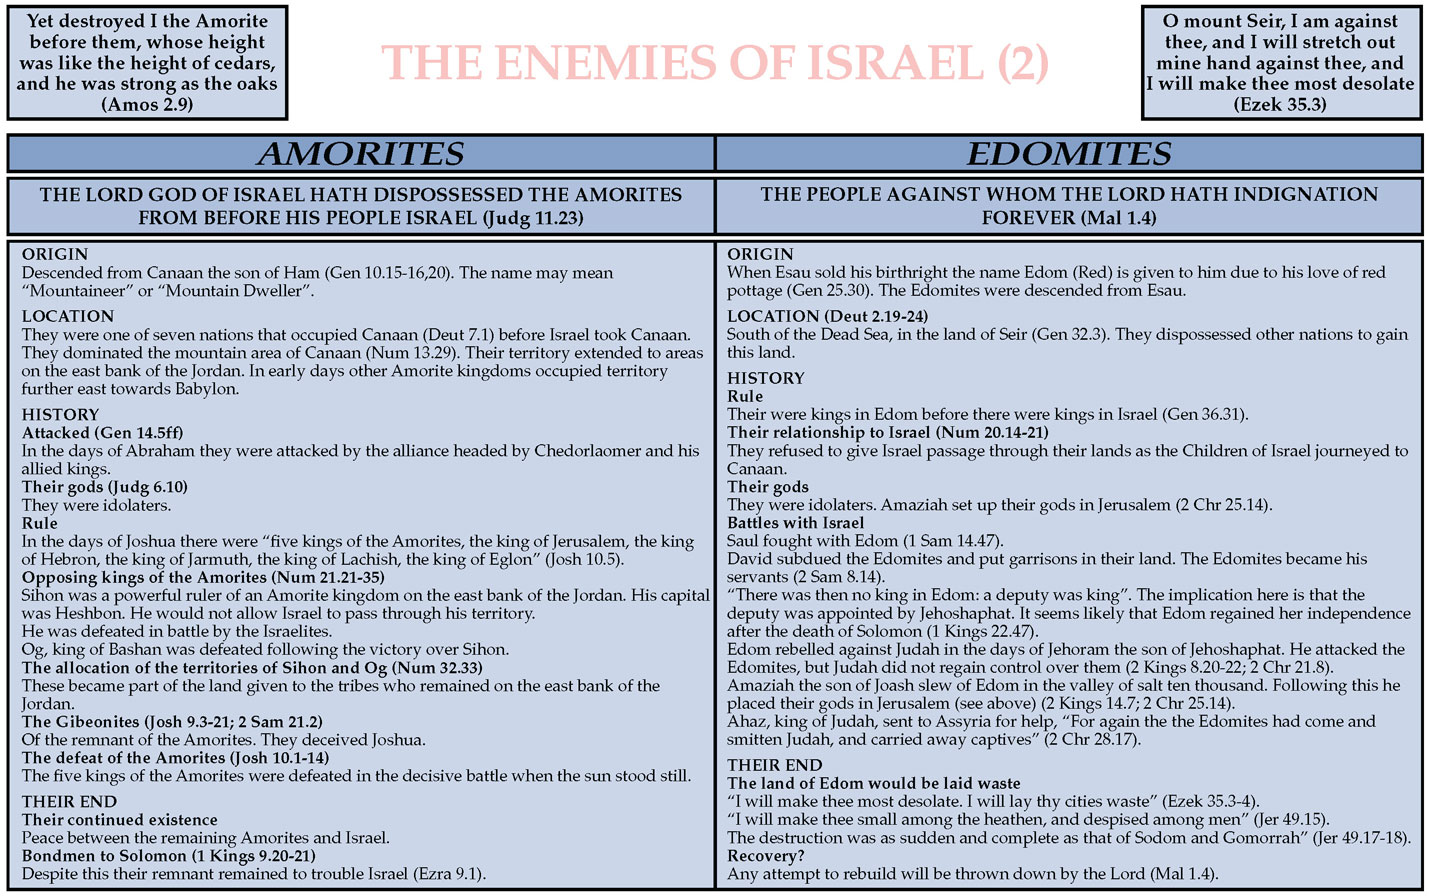
\includegraphics[scale=0.4, angle=90]{06OT-Joshua/References/4.EnemiesOfIsrael2.jpg}
\caption[Enemies of Israel 2]{Enemies of Israel 2}
\label{fig:Enemies of Israel 2}
\end{center}
\end{figure}

\newpage
\begin{figure}
\begin{center}
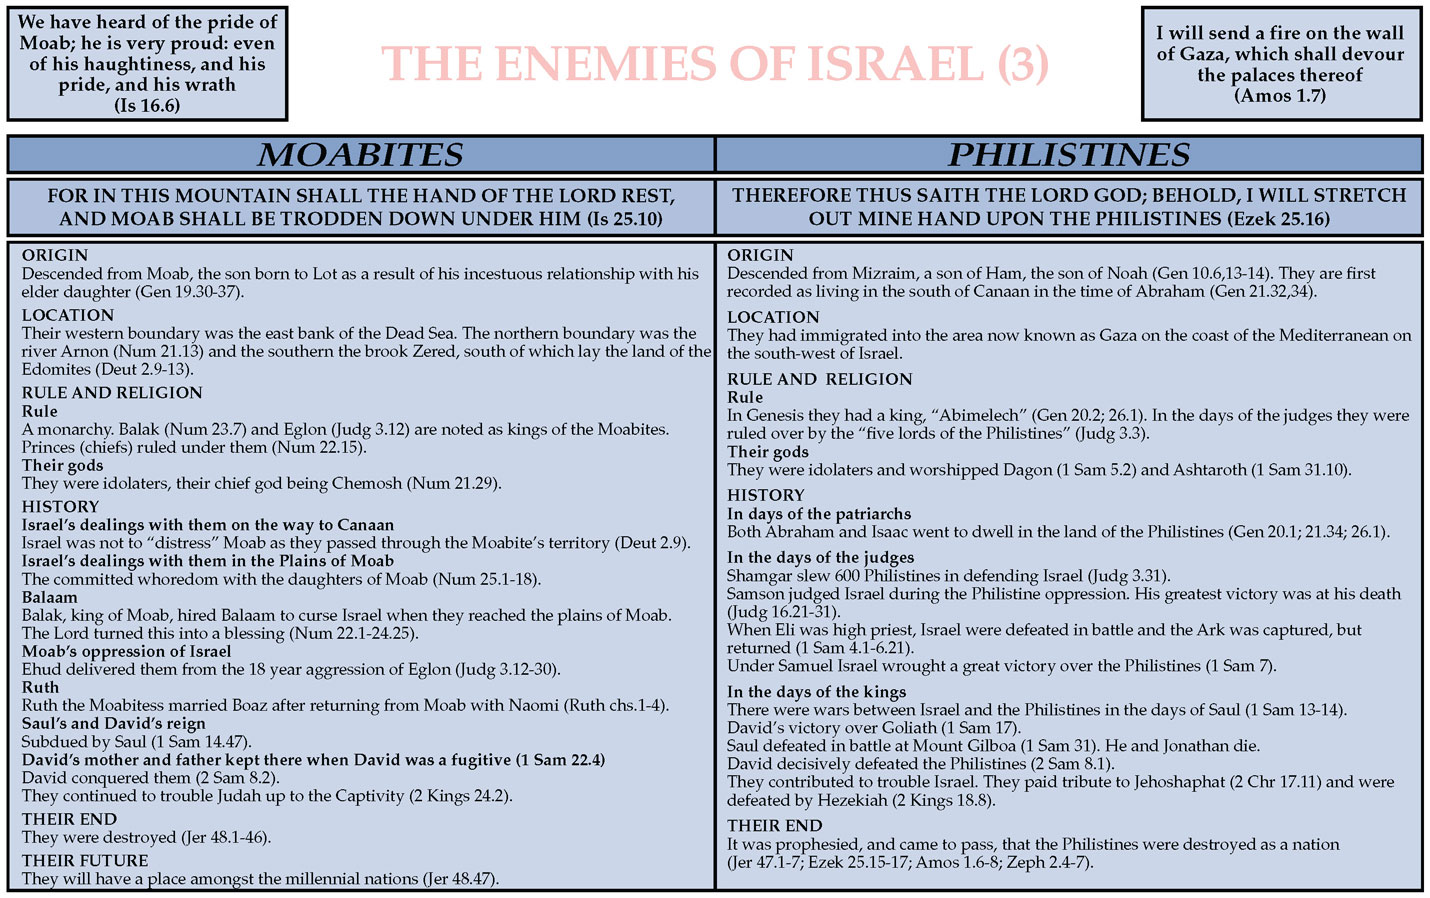
\includegraphics[scale=0.4, angle=90]{06OT-Joshua/References/5.EnemiesOfIsrael3.jpg}
\caption[Enemies of Israel 3]{Enemies of Israel 3}
\label{fig:Enemies of Israel 3}
\end{center}
\end{figure}

\newpage
\begin{figure}
\begin{center}
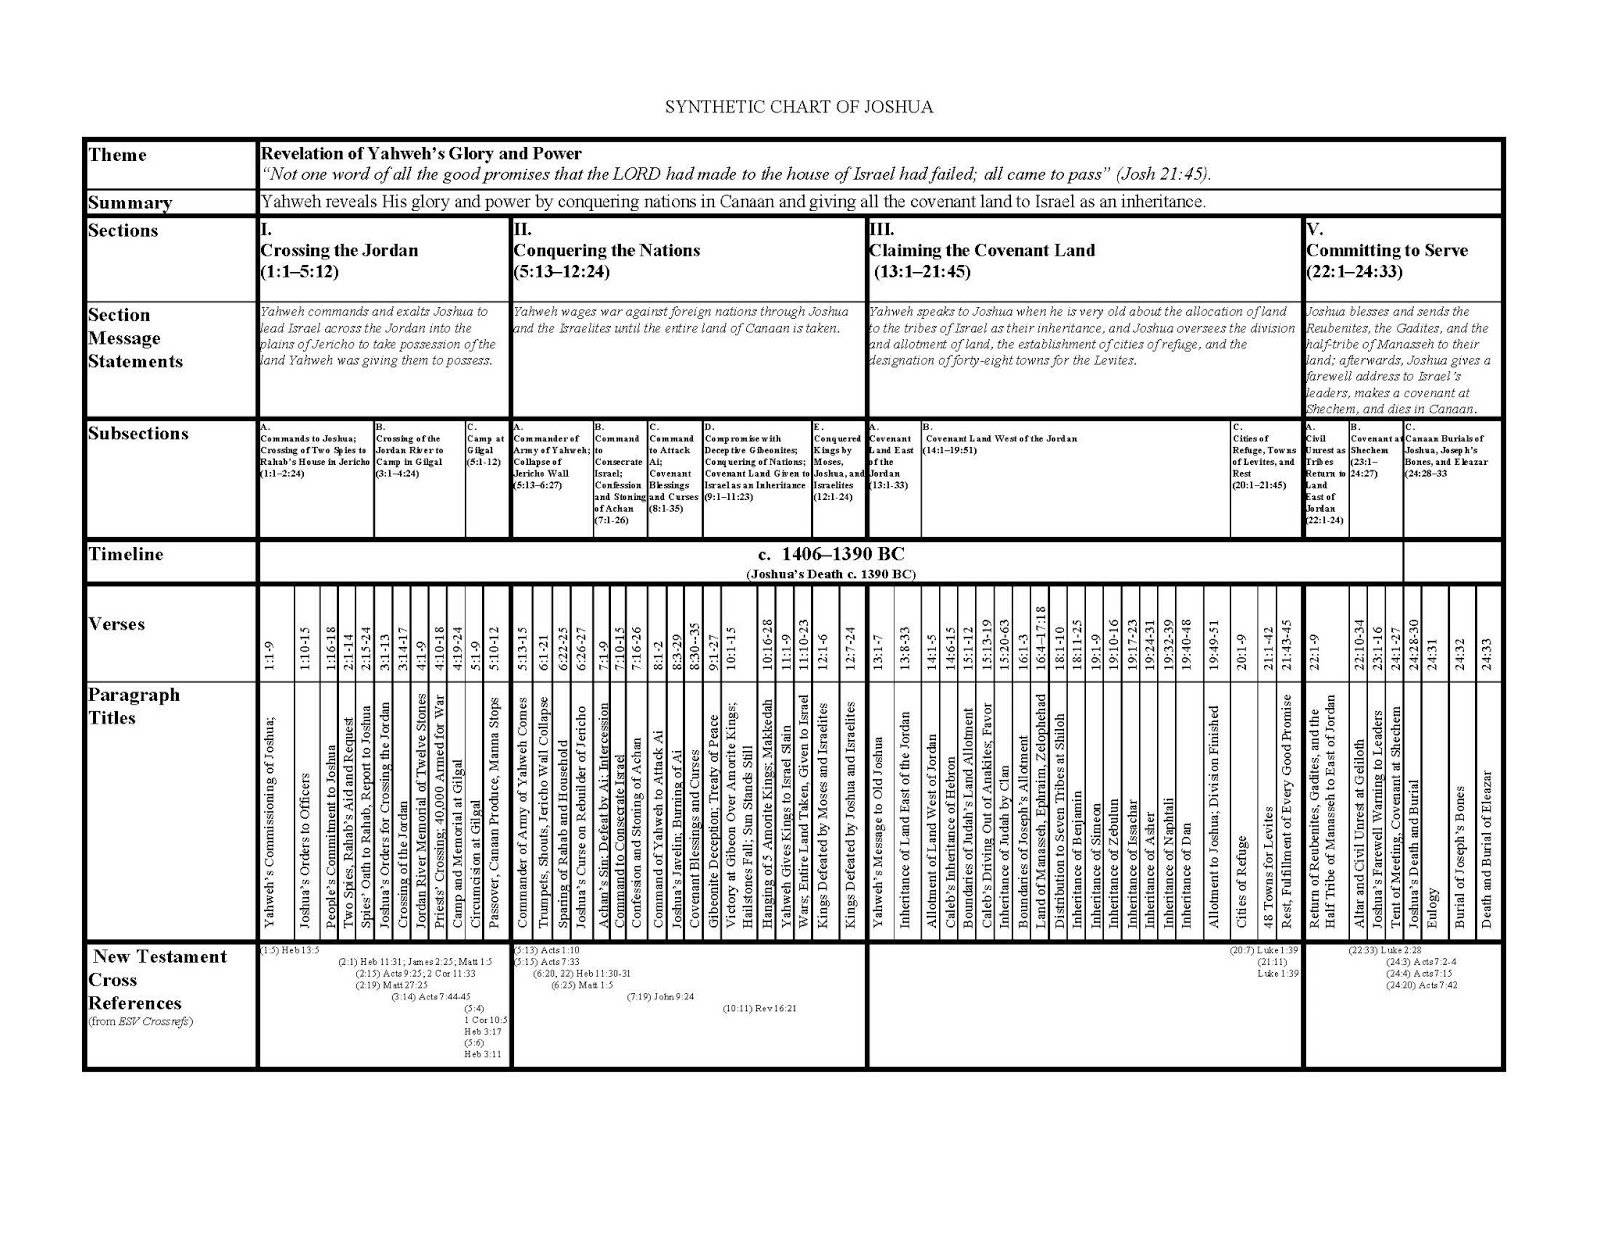
\includegraphics[scale=.4, angle=90]{06OT-Joshua/References/6.SyntheticChartofJoshua.jpg}
\caption[Synthetic Chart of Joshua]{Synthetic Chart of Joshua}
\label{fig:Synthetic Chart of Joshua}
\end{center}
\end{figure}


\newpage
\begin{figure}
\begin{center}
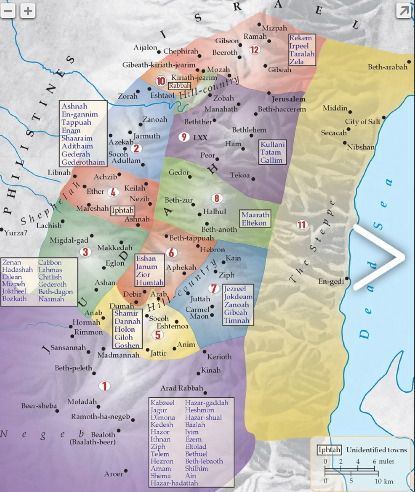
\includegraphics[scale=1, angle=0]{06OT-Joshua/References/7.WestSideOfDeadSea.jpg}
\caption[The West Side of the Dead Sea]{The West Side of the Dead Sea}
\label{fig:The West Side of the Dead Sea}
\end{center}
\end{figure}


\newpage
\begin{figure}
\begin{center}
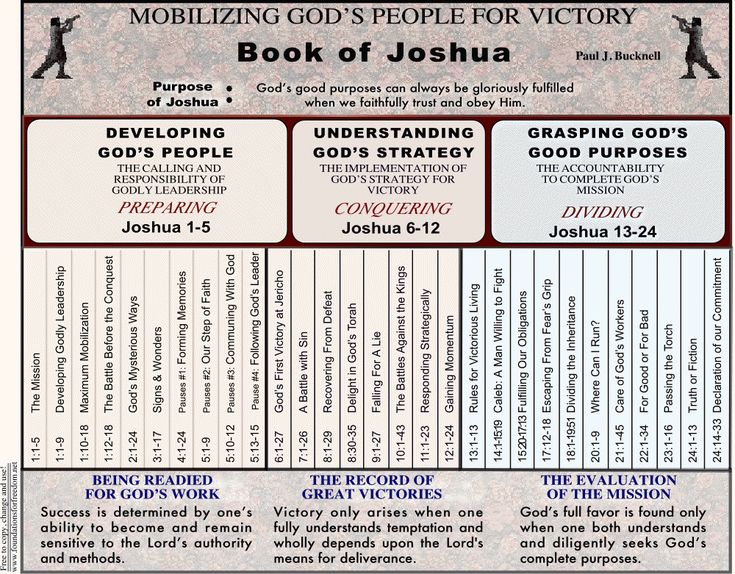
\includegraphics[scale=0.75, angle=90]{06OT-Joshua/References/8.Bucknell-Joshua.jpg}
\caption[Joshua from Bucknell]{Joshua from Bucknell}
\label{fig:Joshua from Bucknell}
\end{center}
\end{figure}


\newpage
\begin{figure}
\begin{center}
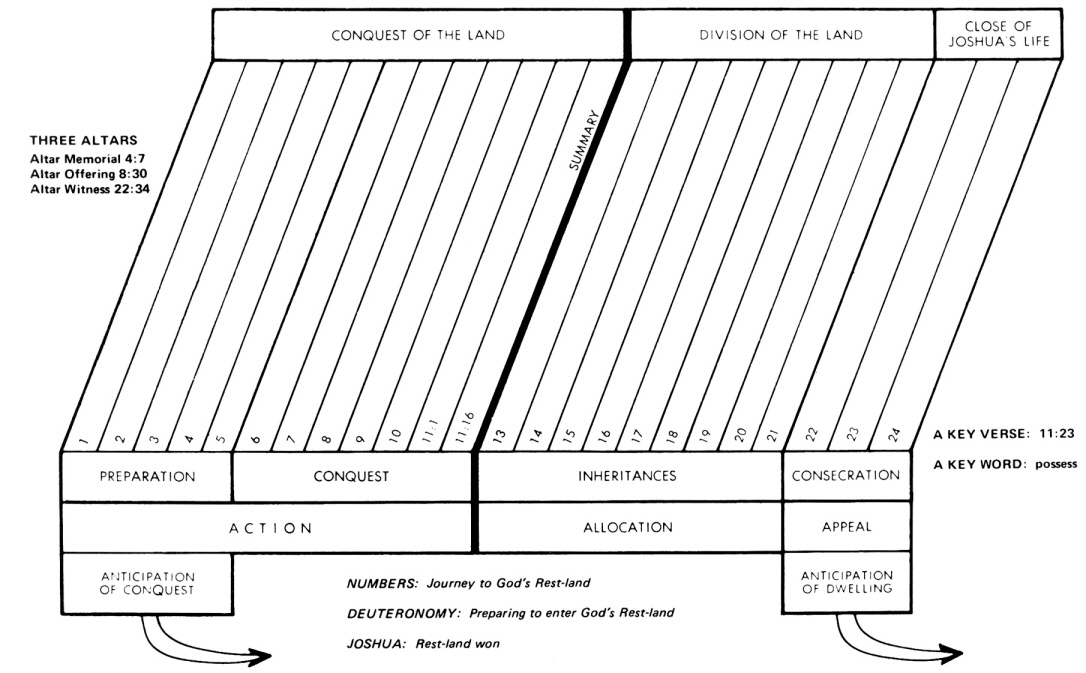
\includegraphics[scale=2, angle=90]{06OT-Joshua/References/9.Jensen-Joshua.png}
\caption[Joshua from Jensen]{Joshua from Jensen}
\label{fig:Joshua from Jensen}
\end{center}
\end{figure}


\newpage
\begin{figure}
\begin{center}
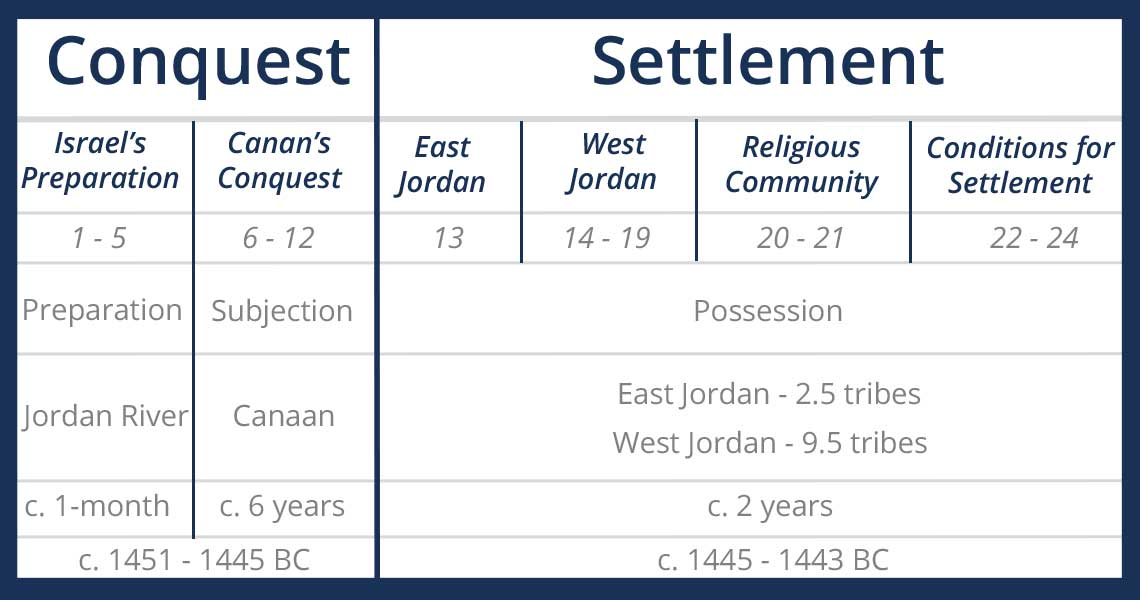
\includegraphics[scale=.5, angle=90]{06OT-Joshua/References/10.Bible-Brief-Joshua.jpg}
\caption[Bible Brief for Joshua]{Bible Brief for Joshua}
\label{fig:Bible Brief for Joshua}
\end{center}
\end{figure}

\newpage
\begin{figure}
\begin{center}
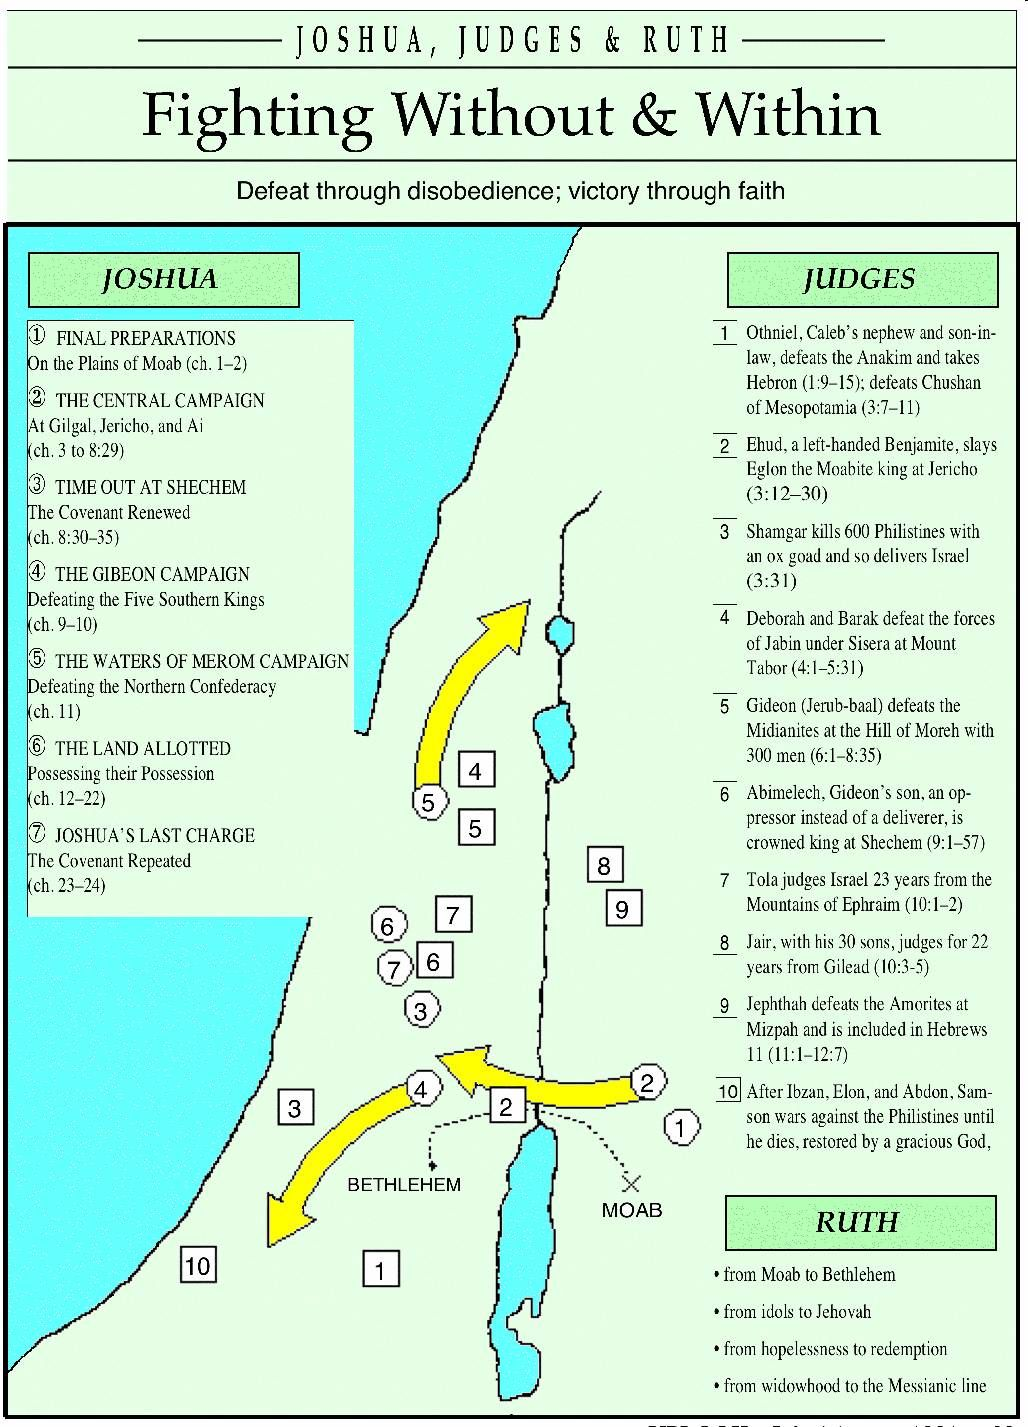
\includegraphics[scale=.5, angle=0]{06OT-Joshua/References/11.FightingInJoshuaAndJudges.jpg}
\caption[The Fighting in Joshua and Judges]{The Fighting in Joshua and Judges}
\label{fig:The Fighting in Joshua and Judges}
\end{center}
\end{figure}

\newpage
\begin{figure}
\begin{center}
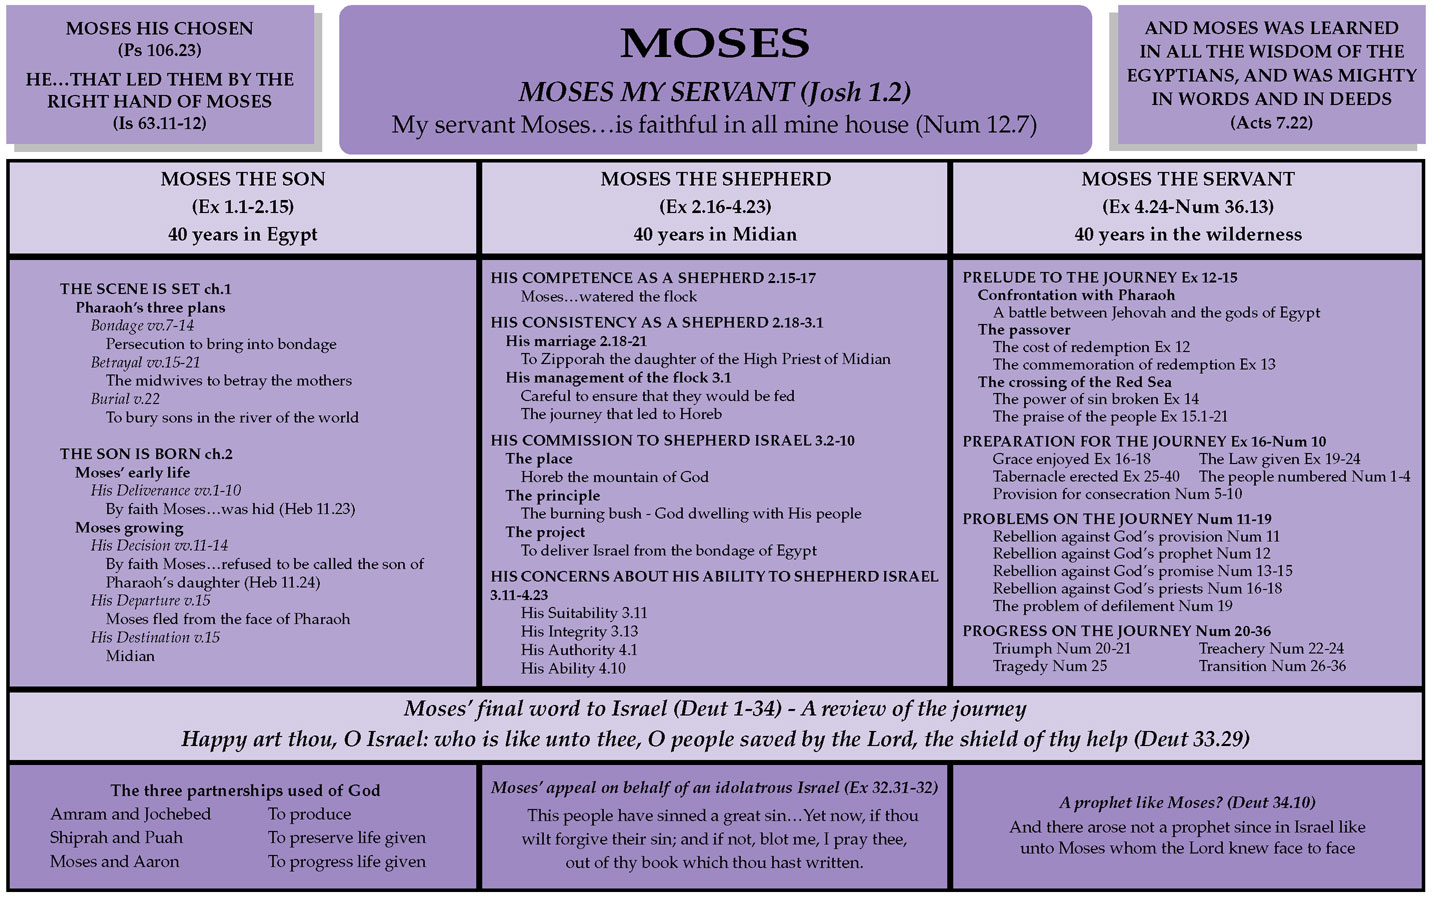
\includegraphics[scale=.4, angle=90]{06OT-Joshua/References/12.JohnGrantMoses.jpg}
\caption[Moses from John Grant]{Moses from John Grant}
\label{fig:Moses from John Grant}
\end{center}
\end{figure}








\chapter{Joshua 16}

\begin{figure}
  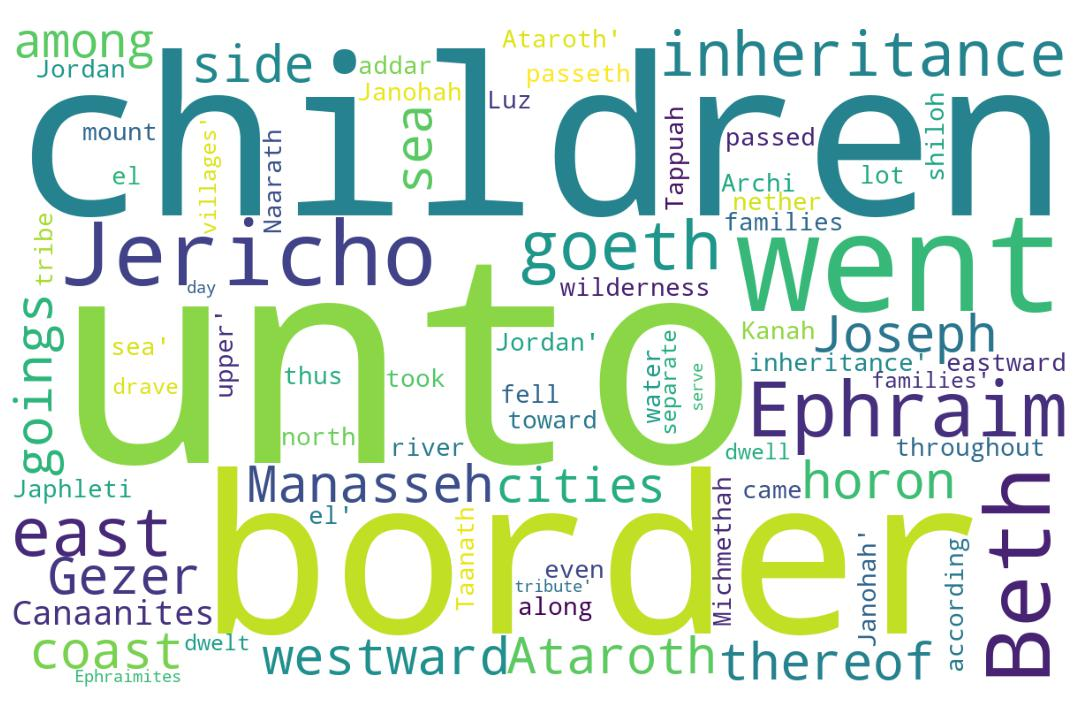
\includegraphics[width=\linewidth]{06OT-Joshua/Joshua16-WordCloud.jpg}
  \caption{Joshua 16 Word Cloud}
  \label{fig:Joshua 16 Word Cloud}
\end{figure}


\marginpar{\scriptsize \centering \fcolorbox{bone}{lime}{\textbf{LAND FOR THE SONS OF JOSEPH}}\\ (Joshua 16:1-10) \begin{compactenum}[I.][8]
	\item The \textbf{Sons}  \index[scripture]{Joshua!Jsh 16:01}  (Jsh 16:1) 
	\item \textbf{Sides of the Compass}  \index[scripture]{Joshua!Jsh 16:02--03}  (Jsh 16:2--3) 
	\item \textbf{Shiloh}  \index[scripture]{Joshua!Jsh 16:06}  (Jsh 16:6) 
	\item The \textbf{Sea} as a Border \index[scripture]{Joshua!Jsh 16:08}  (Jsh 16:8) 
	\item The \textbf{Separate Cities}  \index[scripture]{Joshua!Jsh 16:09}  (Jsh 16:9) 
	\item \textbf{Squatters}  \index[scripture]{Joshua!Jsh 16:10}  (Jsh 16:10) 
	\item Like \textbf{Sin}  \index[scripture]{Joshua!Jsh 16:10}  (Jsh 16:10) 
\end{compactenum}}



\footnote{\textcolor[cmyk]{0.99998,1,0,0}{\hyperlink{TOC}{Return to end of Table of Contents.}}}\footnote{\href{https://audiobible.com/bible/joshua_16.html}{\textcolor[cmyk]{0.99998,1,0,0}{Joshua 16 Audio}}}\textcolor[cmyk]{0.99998,1,0,0}{And the lot of the \fcolorbox{bone}{lime}{children of Joseph} fell from Jordan by Jericho, unto the water of Jericho on the east, to the wilderness that goeth up from Jericho throughout mount Beth-el,} 
[2] \textcolor[cmyk]{0.99998,1,0,0}{And goeth out from Beth-el to Luz, and passeth along unto the borders of Archi to Ataroth,} 
[3] \textcolor[cmyk]{0.99998,1,0,0}{And goeth down westward to the coast of Japhleti, unto the coast of Beth-horon the nether, and to Gezer: and the goings out thereof are at the sea.}
[4] \textcolor[cmyk]{0.99998,1,0,0}{So the children of Joseph, Manasseh and Ephraim, took their inheritance.}\\
\\
\P \textcolor[cmyk]{0.99998,1,0,0}{And the border of the children of Ephraim according to their families was \emph{thus}: even the border of their inheritance on the east side was Ataroth-addar, unto Beth-horon the upper;}
[6] \textcolor[cmyk]{0.99998,1,0,0}{And the border went out toward the sea to Michmethah on the north side; and the border went about eastward unto \fcolorbox{bone}{lime}{Taanath-shiloh}, and passed by it on the east to Janohah;} 
[7] \textcolor[cmyk]{0.99998,1,0,0}{And it went down from Janohah to Ataroth, and to Naarath, and came to Jericho, and went out at Jordan.}
[8] \textcolor[cmyk]{0.99998,1,0,0}{The border went out from Tappuah westward unto the river Kanah; and the goings out thereof were at the \fcolorbox{bone}{lime}{sea}. This \emph{is} the inheritance of the tribe of the children of Ephraim by their families.}
[9] \textcolor[cmyk]{0.99998,1,0,0}{And the \fcolorbox{bone}{lime}{separate cities} for the children of Ephraim \emph{were} among the inheritance of the children of Manasseh, all the cities with their villages.} 
[10] \textcolor[cmyk]{0.99998,1,0,0}{And they drave not out the Canaanites that dwelt in Gezer: but the \fcolorbox{bone}{lime}{Canaanites dwell} among the Ephraimites unto this day, and serve under tribute.} 

\index[NWIV]{32!Joshua!Jos 16:1}\index[AWIP]{And!Joshua!Jos 16:1}\index[AWIP]{the!Joshua!Jos 16:1}\index[AWIP]{the!Joshua!Jos 16:1 (2)}\index[AWIP]{the!Joshua!Jos 16:1 (3)}\index[AWIP]{the!Joshua!Jos 16:1 (4)}\index[AWIP]{the!Joshua!Jos 16:1 (5)}\index[AWIP]{lot!Joshua!Jos 16:1}\index[AWIP]{of!Joshua!Jos 16:1}\index[AWIP]{of!Joshua!Jos 16:1 (2)}\index[AWIP]{of!Joshua!Jos 16:1 (3)}\index[AWIP]{children!Joshua!Jos 16:1}\index[AWIP]{Joseph!Joshua!Jos 16:1}\index[AWIP]{fell!Joshua!Jos 16:1}\index[AWIP]{from!Joshua!Jos 16:1}\index[AWIP]{from!Joshua!Jos 16:1 (2)}\index[AWIP]{Jordan!Joshua!Jos 16:1}\index[AWIP]{by!Joshua!Jos 16:1}\index[AWIP]{Jericho!Joshua!Jos 16:1}\index[AWIP]{Jericho!Joshua!Jos 16:1 (2)}\index[AWIP]{Jericho!Joshua!Jos 16:1 (3)}\index[AWIP]{unto!Joshua!Jos 16:1}\index[AWIP]{water!Joshua!Jos 16:1}\index[AWIP]{on!Joshua!Jos 16:1}\index[AWIP]{east!Joshua!Jos 16:1}\index[AWIP]{to!Joshua!Jos 16:1}\index[AWIP]{wilderness!Joshua!Jos 16:1}\index[AWIP]{that!Joshua!Jos 16:1}\index[AWIP]{goeth!Joshua!Jos 16:1}\index[AWIP]{up!Joshua!Jos 16:1}\index[AWIP]{throughout!Joshua!Jos 16:1}\index[AWIP]{mount!Joshua!Jos 16:1}\index[AWIP]{Beth-el!Joshua!Jos 16:1}

\index[NWIV]{17!Joshua!Jos 16:2}\index[AWIP]{And!Joshua!Jos 16:2}\index[AWIP]{goeth!Joshua!Jos 16:2}\index[AWIP]{out!Joshua!Jos 16:2}\index[AWIP]{from!Joshua!Jos 16:2}\index[AWIP]{Beth-el!Joshua!Jos 16:2}\index[AWIP]{to!Joshua!Jos 16:2}\index[AWIP]{to!Joshua!Jos 16:2 (2)}\index[AWIP]{Luz!Joshua!Jos 16:2}\index[AWIP]{and!Joshua!Jos 16:2}\index[AWIP]{passeth!Joshua!Jos 16:2}\index[AWIP]{along!Joshua!Jos 16:2}\index[AWIP]{unto!Joshua!Jos 16:2}\index[AWIP]{the!Joshua!Jos 16:2}\index[AWIP]{borders!Joshua!Jos 16:2}\index[AWIP]{of!Joshua!Jos 16:2}\index[AWIP]{Archi!Joshua!Jos 16:2}\index[AWIP]{Ataroth!Joshua!Jos 16:2}

\index[NWIV]{28!Joshua!Jos 16:3}\index[AWIP]{And!Joshua!Jos 16:3}\index[AWIP]{goeth!Joshua!Jos 16:3}\index[AWIP]{down!Joshua!Jos 16:3}\index[AWIP]{westward!Joshua!Jos 16:3}\index[AWIP]{to!Joshua!Jos 16:3}\index[AWIP]{to!Joshua!Jos 16:3 (2)}\index[AWIP]{the!Joshua!Jos 16:3}\index[AWIP]{the!Joshua!Jos 16:3 (2)}\index[AWIP]{the!Joshua!Jos 16:3 (3)}\index[AWIP]{the!Joshua!Jos 16:3 (4)}\index[AWIP]{the!Joshua!Jos 16:3 (5)}\index[AWIP]{coast!Joshua!Jos 16:3}\index[AWIP]{coast!Joshua!Jos 16:3 (2)}\index[AWIP]{of!Joshua!Jos 16:3}\index[AWIP]{of!Joshua!Jos 16:3 (2)}\index[AWIP]{Japhleti!Joshua!Jos 16:3}\index[AWIP]{unto!Joshua!Jos 16:3}\index[AWIP]{Beth-horon!Joshua!Jos 16:3}\index[AWIP]{nether!Joshua!Jos 16:3}\index[AWIP]{and!Joshua!Jos 16:3}\index[AWIP]{and!Joshua!Jos 16:3 (2)}\index[AWIP]{Gezer!Joshua!Jos 16:3}\index[AWIP]{goings!Joshua!Jos 16:3}\index[AWIP]{out!Joshua!Jos 16:3}\index[AWIP]{thereof!Joshua!Jos 16:3}\index[AWIP]{are!Joshua!Jos 16:3}\index[AWIP]{at!Joshua!Jos 16:3}\index[AWIP]{sea!Joshua!Jos 16:3}

\index[NWIV]{11!Joshua!Jos 16:4}\index[AWIP]{So!Joshua!Jos 16:4}\index[AWIP]{the!Joshua!Jos 16:4}\index[AWIP]{children!Joshua!Jos 16:4}\index[AWIP]{of!Joshua!Jos 16:4}\index[AWIP]{Joseph!Joshua!Jos 16:4}\index[AWIP]{Manasseh!Joshua!Jos 16:4}\index[AWIP]{and!Joshua!Jos 16:4}\index[AWIP]{Ephraim!Joshua!Jos 16:4}\index[AWIP]{took!Joshua!Jos 16:4}\index[AWIP]{their!Joshua!Jos 16:4}\index[AWIP]{inheritance!Joshua!Jos 16:4}

\index[NWIV]{30!Joshua!Jos 16:5}\index[AWIP]{And!Joshua!Jos 16:5}\index[AWIP]{the!Joshua!Jos 16:5}\index[AWIP]{the!Joshua!Jos 16:5 (2)}\index[AWIP]{the!Joshua!Jos 16:5 (3)}\index[AWIP]{the!Joshua!Jos 16:5 (4)}\index[AWIP]{the!Joshua!Jos 16:5 (5)}\index[AWIP]{border!Joshua!Jos 16:5}\index[AWIP]{border!Joshua!Jos 16:5 (2)}\index[AWIP]{of!Joshua!Jos 16:5}\index[AWIP]{of!Joshua!Jos 16:5 (2)}\index[AWIP]{of!Joshua!Jos 16:5 (3)}\index[AWIP]{children!Joshua!Jos 16:5}\index[AWIP]{Ephraim!Joshua!Jos 16:5}\index[AWIP]{according!Joshua!Jos 16:5}\index[AWIP]{to!Joshua!Jos 16:5}\index[AWIP]{their!Joshua!Jos 16:5}\index[AWIP]{their!Joshua!Jos 16:5 (2)}\index[AWIP]{families!Joshua!Jos 16:5}\index[AWIP]{was!Joshua!Jos 16:5}\index[AWIP]{was!Joshua!Jos 16:5 (2)}\index[AWIP]{\emph{thus}!Joshua!Jos 16:5}\index[AWIP]{even!Joshua!Jos 16:5}\index[AWIP]{inheritance!Joshua!Jos 16:5}\index[AWIP]{on!Joshua!Jos 16:5}\index[AWIP]{east!Joshua!Jos 16:5}\index[AWIP]{side!Joshua!Jos 16:5}\index[AWIP]{Ataroth-addar!Joshua!Jos 16:5}\index[AWIP]{unto!Joshua!Jos 16:5}\index[AWIP]{Beth-horon!Joshua!Jos 16:5}\index[AWIP]{upper!Joshua!Jos 16:5}\index[AWIP]{\emph{thus}!Joshua!Jos 16:5}

\index[NWIV]{31!Joshua!Jos 16:6}\index[AWIP]{And!Joshua!Jos 16:6}\index[AWIP]{the!Joshua!Jos 16:6}\index[AWIP]{the!Joshua!Jos 16:6 (2)}\index[AWIP]{the!Joshua!Jos 16:6 (3)}\index[AWIP]{the!Joshua!Jos 16:6 (4)}\index[AWIP]{the!Joshua!Jos 16:6 (5)}\index[AWIP]{border!Joshua!Jos 16:6}\index[AWIP]{border!Joshua!Jos 16:6 (2)}\index[AWIP]{went!Joshua!Jos 16:6}\index[AWIP]{went!Joshua!Jos 16:6 (2)}\index[AWIP]{out!Joshua!Jos 16:6}\index[AWIP]{toward!Joshua!Jos 16:6}\index[AWIP]{sea!Joshua!Jos 16:6}\index[AWIP]{to!Joshua!Jos 16:6}\index[AWIP]{to!Joshua!Jos 16:6 (2)}\index[AWIP]{Michmethah!Joshua!Jos 16:6}\index[AWIP]{on!Joshua!Jos 16:6}\index[AWIP]{on!Joshua!Jos 16:6 (2)}\index[AWIP]{north!Joshua!Jos 16:6}\index[AWIP]{side!Joshua!Jos 16:6}\index[AWIP]{and!Joshua!Jos 16:6}\index[AWIP]{and!Joshua!Jos 16:6 (2)}\index[AWIP]{about!Joshua!Jos 16:6}\index[AWIP]{eastward!Joshua!Jos 16:6}\index[AWIP]{unto!Joshua!Jos 16:6}\index[AWIP]{Taanath-shiloh!Joshua!Jos 16:6}\index[AWIP]{passed!Joshua!Jos 16:6}\index[AWIP]{by!Joshua!Jos 16:6}\index[AWIP]{it!Joshua!Jos 16:6}\index[AWIP]{east!Joshua!Jos 16:6}\index[AWIP]{Janohah!Joshua!Jos 16:6}

\index[NWIV]{20!Joshua!Jos 16:7}\index[AWIP]{And!Joshua!Jos 16:7}\index[AWIP]{it!Joshua!Jos 16:7}\index[AWIP]{went!Joshua!Jos 16:7}\index[AWIP]{went!Joshua!Jos 16:7 (2)}\index[AWIP]{down!Joshua!Jos 16:7}\index[AWIP]{from!Joshua!Jos 16:7}\index[AWIP]{Janohah!Joshua!Jos 16:7}\index[AWIP]{to!Joshua!Jos 16:7}\index[AWIP]{to!Joshua!Jos 16:7 (2)}\index[AWIP]{to!Joshua!Jos 16:7 (3)}\index[AWIP]{Ataroth!Joshua!Jos 16:7}\index[AWIP]{and!Joshua!Jos 16:7}\index[AWIP]{and!Joshua!Jos 16:7 (2)}\index[AWIP]{and!Joshua!Jos 16:7 (3)}\index[AWIP]{Naarath!Joshua!Jos 16:7}\index[AWIP]{came!Joshua!Jos 16:7}\index[AWIP]{Jericho!Joshua!Jos 16:7}\index[AWIP]{out!Joshua!Jos 16:7}\index[AWIP]{at!Joshua!Jos 16:7}\index[AWIP]{Jordan!Joshua!Jos 16:7}

\index[NWIV]{35!Joshua!Jos 16:8}\index[AWIP]{The!Joshua!Jos 16:8}\index[AWIP]{border!Joshua!Jos 16:8}\index[AWIP]{went!Joshua!Jos 16:8}\index[AWIP]{out!Joshua!Jos 16:8}\index[AWIP]{out!Joshua!Jos 16:8 (2)}\index[AWIP]{from!Joshua!Jos 16:8}\index[AWIP]{Tappuah!Joshua!Jos 16:8}\index[AWIP]{westward!Joshua!Jos 16:8}\index[AWIP]{unto!Joshua!Jos 16:8}\index[AWIP]{the!Joshua!Jos 16:8}\index[AWIP]{the!Joshua!Jos 16:8 (2)}\index[AWIP]{the!Joshua!Jos 16:8 (3)}\index[AWIP]{the!Joshua!Jos 16:8 (4)}\index[AWIP]{the!Joshua!Jos 16:8 (5)}\index[AWIP]{the!Joshua!Jos 16:8 (6)}\index[AWIP]{river!Joshua!Jos 16:8}\index[AWIP]{Kanah!Joshua!Jos 16:8}\index[AWIP]{and!Joshua!Jos 16:8}\index[AWIP]{goings!Joshua!Jos 16:8}\index[AWIP]{thereof!Joshua!Jos 16:8}\index[AWIP]{were!Joshua!Jos 16:8}\index[AWIP]{at!Joshua!Jos 16:8}\index[AWIP]{sea!Joshua!Jos 16:8}\index[AWIP]{This!Joshua!Jos 16:8}\index[AWIP]{\emph{is}!Joshua!Jos 16:8}\index[AWIP]{inheritance!Joshua!Jos 16:8}\index[AWIP]{of!Joshua!Jos 16:8}\index[AWIP]{of!Joshua!Jos 16:8 (2)}\index[AWIP]{of!Joshua!Jos 16:8 (3)}\index[AWIP]{tribe!Joshua!Jos 16:8}\index[AWIP]{children!Joshua!Jos 16:8}\index[AWIP]{Ephraim!Joshua!Jos 16:8}\index[AWIP]{by!Joshua!Jos 16:8}\index[AWIP]{their!Joshua!Jos 16:8}\index[AWIP]{families!Joshua!Jos 16:8}\index[AWIP]{\emph{is}!Joshua!Jos 16:8}

\index[NWIV]{24!Joshua!Jos 16:9}\index[AWIP]{And!Joshua!Jos 16:9}\index[AWIP]{the!Joshua!Jos 16:9}\index[AWIP]{the!Joshua!Jos 16:9 (2)}\index[AWIP]{the!Joshua!Jos 16:9 (3)}\index[AWIP]{the!Joshua!Jos 16:9 (4)}\index[AWIP]{the!Joshua!Jos 16:9 (5)}\index[AWIP]{separate!Joshua!Jos 16:9}\index[AWIP]{cities!Joshua!Jos 16:9}\index[AWIP]{cities!Joshua!Jos 16:9 (2)}\index[AWIP]{for!Joshua!Jos 16:9}\index[AWIP]{children!Joshua!Jos 16:9}\index[AWIP]{children!Joshua!Jos 16:9 (2)}\index[AWIP]{of!Joshua!Jos 16:9}\index[AWIP]{of!Joshua!Jos 16:9 (2)}\index[AWIP]{of!Joshua!Jos 16:9 (3)}\index[AWIP]{Ephraim!Joshua!Jos 16:9}\index[AWIP]{\emph{were}!Joshua!Jos 16:9}\index[AWIP]{among!Joshua!Jos 16:9}\index[AWIP]{inheritance!Joshua!Jos 16:9}\index[AWIP]{Manasseh!Joshua!Jos 16:9}\index[AWIP]{all!Joshua!Jos 16:9}\index[AWIP]{with!Joshua!Jos 16:9}\index[AWIP]{their!Joshua!Jos 16:9}\index[AWIP]{villages!Joshua!Jos 16:9}\index[AWIP]{\emph{were}!Joshua!Jos 16:9}

\index[NWIV]{25!Joshua!Jos 16:10}\index[AWIP]{And!Joshua!Jos 16:10}\index[AWIP]{they!Joshua!Jos 16:10}\index[AWIP]{drave!Joshua!Jos 16:10}\index[AWIP]{not!Joshua!Jos 16:10}\index[AWIP]{out!Joshua!Jos 16:10}\index[AWIP]{the!Joshua!Jos 16:10}\index[AWIP]{the!Joshua!Jos 16:10 (2)}\index[AWIP]{the!Joshua!Jos 16:10 (3)}\index[AWIP]{Canaanites!Joshua!Jos 16:10}\index[AWIP]{Canaanites!Joshua!Jos 16:10 (2)}\index[AWIP]{that!Joshua!Jos 16:10}\index[AWIP]{dwelt!Joshua!Jos 16:10}\index[AWIP]{in!Joshua!Jos 16:10}\index[AWIP]{Gezer!Joshua!Jos 16:10}\index[AWIP]{but!Joshua!Jos 16:10}\index[AWIP]{dwell!Joshua!Jos 16:10}\index[AWIP]{among!Joshua!Jos 16:10}\index[AWIP]{Ephraimites!Joshua!Jos 16:10}\index[AWIP]{unto!Joshua!Jos 16:10}\index[AWIP]{this!Joshua!Jos 16:10}\index[AWIP]{day!Joshua!Jos 16:10}\index[AWIP]{and!Joshua!Jos 16:10}\index[AWIP]{serve!Joshua!Jos 16:10}\index[AWIP]{under!Joshua!Jos 16:10}\index[AWIP]{tribute!Joshua!Jos 16:10}


\section{Joshua 16 Outlines}

\subsection{My Outlines}

\subsubsection{Land for the Sons of Joseph}
\index[speaker]{Keith Anthony!Joshua 16 (Land for the Sons of Joseph}
\index[series]{Joshua (Keith Anthony)!Joshua 16 (Land for the Sons of Joseph)}
\index[date]{2018/03/12!Joshua 16 (Land for the Sons of Joseph) (Keith Anthony)}
\begin{compactenum}[I.]
	\item The \textbf{Sons}  \index[scripture]{Joshua!Jsh 16:01}  (Jsh 16:1) 
	\item \textbf{Sides of the Compass}  \index[scripture]{Joshua!Jsh 16:02--03}  (Jsh 16:2--3) 
	\item \textbf{Shiloh}  \index[scripture]{Joshua!Jsh 16:06}  (Jsh 16:6) 
	\item The \textbf{Sea} as a Border \index[scripture]{Joshua!Jsh 16:08}  (Jsh 16:8) 
	\item The \textbf{Separate Cities}  \index[scripture]{Joshua!Jsh 16:09}  (Jsh 16:9) 
	\item \textbf{Squatters}  \index[scripture]{Joshua!Jsh 16:10}  (Jsh 16:10) 
	\item Like \textbf{Sin}  \index[scripture]{Joshua!Jsh 16:10}  (Jsh 16:10) 
\end{compactenum}
\subsection{My Outlines from Others}


\section{Joshua 16 Comments}

\subsection{numeric Nuggets}
\textbf{13: } The 13-character name ``Ataroth-addar'' is foudn in verse 5.
\subsection{Joshua 16 Repeated Phrases}


%%%%%%%%%%
%%%%%%%%%%
\normalsize
 
\begin{center}
\begin{longtable}{|p{3.0in}|p{0.5in}|}
\caption[Joshua 16 Repeated Phrases]{Joshua 16 Repeated Phrases}\label{table:Repeated Phrases Joshua 16} \\
\hline \multicolumn{1}{|c|}{\textbf{Phrase}} & \multicolumn{1}{c|}{\textbf{Frequency}} \\ \hline 
\endfirsthead
 
\multicolumn{2}{c}
{{\bfseries \tablename\ \thetable{} -- continued from previous page}} \\  
\hline \multicolumn{1}{|c|}{\textbf{Phrase}} & \multicolumn{1}{c|}{\textbf{Frequency}} \\ \hline 
\endhead
 
\hline \multicolumn{2}{c}{{ }} \\ \hline
\endfoot 
the children & 6\\ \hline 
the children of & 6\\ \hline 
children of & 6\\ \hline 
of the & 5\\ \hline 
And the & 4\\ \hline 
of the children & 4\\ \hline 
of the children of & 4\\ \hline 
unto the & 4\\ \hline 
on the & 4\\ \hline 
the border & 4\\ \hline 
on the east & 3\\ \hline 
the east & 3\\ \hline 
and the & 3\\ \hline 
the sea & 3\\ \hline 
the children of Ephraim & 3\\ \hline 
children of Ephraim & 3\\ \hline 
of Ephraim & 3\\ \hline 
border went & 3\\ \hline 
went out & 3\\ \hline 
\end{longtable}
\end{center}



%%%%%%%%%%
%%%%%%%%%%



\section{Joshua 16 Statistics}

%%%%%%%%%%%%%%%%%%%%%%%%%%%
%%%%% Word Statistics
%%%%%%%%%%%%%%%%%%%%%%%%%%


\normalsize



\subsection{Chapter Word Statistics}


%%%%%%%%%%
%%%%%%%%%%
 
\begin{center}
\begin{longtable}{l|c|c|c|c}
\caption[Stats for Joshua 16]{Stats for Joshua 16} \label{table:Stats for Joshua 16} \\ 
\hline \multicolumn{1}{|c|}{\textbf{Verse(s)}} & \multicolumn{1}{|c|}{\textbf{Count}} & \multicolumn{1}{|c|}{\textbf{Unique}} & \multicolumn{1}{|c|}{\textbf{Italics}} & \multicolumn{1}{|c|}{\textbf{Uniq Italic}}  \\ \hline 
\endfirsthead
 
\multicolumn{5}{c}
{{\bfseries \tablename\ \thetable{} -- continued from previous page}} \\  
\hline \multicolumn{1}{|c|}{\textbf{Verse(s)}} & \multicolumn{1}{|c|}{\textbf{Count}} & \multicolumn{1}{|c|}{\textbf{Unique}} & \multicolumn{1}{|c|}{\textbf{Italics}} & \multicolumn{1}{|c|}{\textbf{Uniq Italic}}  \\ \hline 
\endhead
 
\hline \multicolumn{5}{|r|}{{Continued if needed}} \\ \hline
\endfoot 
1 & 32 & 23 & 0 & 0\\ \hline
2 & 17 & 16 & 0 & 0\\ \hline
3 & 28 & 20 & 0 & 0\\ \hline
4 & 11 & 11 & 0 & 0\\ \hline
5 & 30 & 21 & 1 & 1\\ \hline
6 & 31 & 22 & 0 & 0\\ \hline
7 & 20 & 15 & 0 & 0\\ \hline
8 & 35 & 27 & 1 & 1\\ \hline
9 & 24 & 16 & 1 & 1\\ \hline
10 & 25 & 22 & 0 & 0\\ \hline
\hline \hline
Total & 253 & 100 & 3 & 3



\end{longtable}
\end{center}

%%%%%%%%%%
%%%%%%%%%%
 
\subsection{Words by Frequency}

\begin{center}
\begin{longtable}{l|r}
\caption[Word Frequencies in Joshua 16]{Word Frequencies in Joshua 16} \label{table:WordsIn-Joshua-16} \\ 
\hline \multicolumn{1}{|c|}{\textbf{Word}} & \multicolumn{1}{c|}{\textbf{Frequency}} \\ \hline 
\endfirsthead
 
\multicolumn{2}{c}
{{\bfseries \tablename\ \thetable{} -- continued from previous page}} \\ 
\hline \multicolumn{1}{|c|}{\textbf{Word}} & \multicolumn{1}{c|}{\textbf{Frequency}} \\ \hline 
\endhead
 
\hline \multicolumn{2}{|r|}{{Continued if needed}} \\ \hline
\endfoot
 
\hline \hline
\endlastfoot
the & 36 \\ \hline
of & 16 \\ \hline
to & 11 \\ \hline
and & 11 \\ \hline
And & 8 \\ \hline
unto & 7 \\ \hline
out & 7 \\ \hline
children & 6 \\ \hline
from & 5 \\ \hline
their & 5 \\ \hline
border & 5 \\ \hline
went & 5 \\ \hline
Jericho & 4 \\ \hline
on & 4 \\ \hline
Ephraim & 4 \\ \hline
inheritance & 4 \\ \hline
by & 3 \\ \hline
east & 3 \\ \hline
goeth & 3 \\ \hline
at & 3 \\ \hline
sea & 3 \\ \hline
Joseph & 2 \\ \hline
Jordan & 2 \\ \hline
that & 2 \\ \hline
Beth-el & 2 \\ \hline
Ataroth & 2 \\ \hline
down & 2 \\ \hline
westward & 2 \\ \hline
coast & 2 \\ \hline
Beth-horon & 2 \\ \hline
Gezer & 2 \\ \hline
goings & 2 \\ \hline
thereof & 2 \\ \hline
Manasseh & 2 \\ \hline
families & 2 \\ \hline
was & 2 \\ \hline
side & 2 \\ \hline
it & 2 \\ \hline
Janohah & 2 \\ \hline
cities & 2 \\ \hline
among & 2 \\ \hline
Canaanites & 2 \\ \hline
lot & 1 \\ \hline
fell & 1 \\ \hline
water & 1 \\ \hline
wilderness & 1 \\ \hline
up & 1 \\ \hline
throughout & 1 \\ \hline
mount & 1 \\ \hline
Luz & 1 \\ \hline
passeth & 1 \\ \hline
along & 1 \\ \hline
borders & 1 \\ \hline
Archi & 1 \\ \hline
Japhleti & 1 \\ \hline
nether & 1 \\ \hline
are & 1 \\ \hline
So & 1 \\ \hline
took & 1 \\ \hline
according & 1 \\ \hline
\emph{thus} & 1 \\ \hline
even & 1 \\ \hline
Ataroth-addar & 1 \\ \hline
upper & 1 \\ \hline
toward & 1 \\ \hline
Michmethah & 1 \\ \hline
north & 1 \\ \hline
about & 1 \\ \hline
eastward & 1 \\ \hline
Taanath-shiloh & 1 \\ \hline
passed & 1 \\ \hline
Naarath & 1 \\ \hline
came & 1 \\ \hline
The & 1 \\ \hline
Tappuah & 1 \\ \hline
river & 1 \\ \hline
Kanah & 1 \\ \hline
were & 1 \\ \hline
This & 1 \\ \hline
\emph{is} & 1 \\ \hline
tribe & 1 \\ \hline
separate & 1 \\ \hline
for & 1 \\ \hline
\emph{were} & 1 \\ \hline
all & 1 \\ \hline
with & 1 \\ \hline
villages & 1 \\ \hline
they & 1 \\ \hline
drave & 1 \\ \hline
not & 1 \\ \hline
dwelt & 1 \\ \hline
in & 1 \\ \hline
but & 1 \\ \hline
dwell & 1 \\ \hline
Ephraimites & 1 \\ \hline
this & 1 \\ \hline
day & 1 \\ \hline
serve & 1 \\ \hline
under & 1 \\ \hline
tribute & 1 \\ \hline
\end{longtable}
\end{center}



\normalsize



\subsection{Words Alphabetically}

\begin{center}
\begin{longtable}{l|r}
\caption[Word Alphabetically in Joshua 16]{Word Alphabetically in Joshua 16} \label{table:WordsIn-Joshua-16} \\ 
\hline \multicolumn{1}{|c|}{\textbf{Word}} & \multicolumn{1}{c|}{\textbf{Frequency}} \\ \hline 
\endfirsthead
 
\multicolumn{2}{c}
{{\bfseries \tablename\ \thetable{} -- continued from previous page}} \\ 
\hline \multicolumn{1}{|c|}{\textbf{Word}} & \multicolumn{1}{c|}{\textbf{Frequency}} \\ \hline 
\endhead
 
\hline \multicolumn{2}{|r|}{{Continued if needed}} \\ \hline
\endfoot
 
\hline \hline
\endlastfoot
And & 8 \\ \hline
Archi & 1 \\ \hline
Ataroth & 2 \\ \hline
Ataroth-addar & 1 \\ \hline
Beth-el & 2 \\ \hline
Beth-horon & 2 \\ \hline
Canaanites & 2 \\ \hline
Ephraim & 4 \\ \hline
Ephraimites & 1 \\ \hline
Gezer & 2 \\ \hline
Janohah & 2 \\ \hline
Japhleti & 1 \\ \hline
Jericho & 4 \\ \hline
Jordan & 2 \\ \hline
Joseph & 2 \\ \hline
Kanah & 1 \\ \hline
Luz & 1 \\ \hline
Manasseh & 2 \\ \hline
Michmethah & 1 \\ \hline
Naarath & 1 \\ \hline
So & 1 \\ \hline
Taanath-shiloh & 1 \\ \hline
Tappuah & 1 \\ \hline
The & 1 \\ \hline
This & 1 \\ \hline
\emph{is} & 1 \\ \hline
\emph{thus} & 1 \\ \hline
\emph{were} & 1 \\ \hline
about & 1 \\ \hline
according & 1 \\ \hline
all & 1 \\ \hline
along & 1 \\ \hline
among & 2 \\ \hline
and & 11 \\ \hline
are & 1 \\ \hline
at & 3 \\ \hline
border & 5 \\ \hline
borders & 1 \\ \hline
but & 1 \\ \hline
by & 3 \\ \hline
came & 1 \\ \hline
children & 6 \\ \hline
cities & 2 \\ \hline
coast & 2 \\ \hline
day & 1 \\ \hline
down & 2 \\ \hline
drave & 1 \\ \hline
dwell & 1 \\ \hline
dwelt & 1 \\ \hline
east & 3 \\ \hline
eastward & 1 \\ \hline
even & 1 \\ \hline
families & 2 \\ \hline
fell & 1 \\ \hline
for & 1 \\ \hline
from & 5 \\ \hline
goeth & 3 \\ \hline
goings & 2 \\ \hline
in & 1 \\ \hline
inheritance & 4 \\ \hline
it & 2 \\ \hline
lot & 1 \\ \hline
mount & 1 \\ \hline
nether & 1 \\ \hline
north & 1 \\ \hline
not & 1 \\ \hline
of & 16 \\ \hline
on & 4 \\ \hline
out & 7 \\ \hline
passed & 1 \\ \hline
passeth & 1 \\ \hline
river & 1 \\ \hline
sea & 3 \\ \hline
separate & 1 \\ \hline
serve & 1 \\ \hline
side & 2 \\ \hline
that & 2 \\ \hline
the & 36 \\ \hline
their & 5 \\ \hline
thereof & 2 \\ \hline
they & 1 \\ \hline
this & 1 \\ \hline
throughout & 1 \\ \hline
to & 11 \\ \hline
took & 1 \\ \hline
toward & 1 \\ \hline
tribe & 1 \\ \hline
tribute & 1 \\ \hline
under & 1 \\ \hline
unto & 7 \\ \hline
up & 1 \\ \hline
upper & 1 \\ \hline
villages & 1 \\ \hline
was & 2 \\ \hline
water & 1 \\ \hline
went & 5 \\ \hline
were & 1 \\ \hline
westward & 2 \\ \hline
wilderness & 1 \\ \hline
with & 1 \\ \hline
\end{longtable}
\end{center}



\normalsize



\subsection{Word Lengths in Chapter}
\normalsize
\begin{longtable}{l|p{3.75in}}
\caption[Words by Length in Joshua 16]{Words by Length in Joshua 16} \label{table:WordsIn-Joshua-16} \\ 
\hline \multicolumn{1}{|c|}{\textbf{Length}} & \multicolumn{1}{c|}{\textbf{Words}} \\ \hline 
\endfirsthead
 
\multicolumn{2}{c}
{{\bfseries \tablename\ \thetable{} -- continued from previous page}} \\ 
\hline \multicolumn{1}{|c|}{\textbf{Length}} & \multicolumn{1}{c|}{\textbf{Words}} \\ \hline 
\endhead
 
\hline \multicolumn{2}{|r|}{{Continued if needed}} \\ \hline
\endfoot
 
\hline \hline
\endlastfoot
2 & of, by, on, to, up, at, So, it, \emph{is}, in \\ \hline
3 & And, the, lot, out, Luz, and, are, sea, was, The, for, all, not, but, day \\ \hline
4 & fell, from, unto, east, that, down, took, \emph{thus}, even, side, went, came, were, This, \emph{were}, with, they, this \\ \hline
5 & water, goeth, mount, along, Archi, coast, Gezer, their, upper, north, about, river, Kanah, tribe, among, drave, dwelt, dwell, serve, under \\ \hline
6 & Joseph, Jordan, nether, goings, border, toward, passed, cities \\ \hline
7 & Jericho, Beth-el, passeth, borders, Ataroth, thereof, Ephraim, Janohah, Naarath, Tappuah, tribute \\ \hline
8 & children, westward, Japhleti, Manasseh, families, eastward, separate, villages \\ \hline
9 & according \\ \hline
10 & wilderness, throughout, Beth-horon, Michmethah, Canaanites \\ \hline
11 & inheritance, Ephraimites \\ \hline
13 & Ataroth-addar \\ \hline
14 & Taanath-shiloh \\ \hline
\end{longtable}






%%%%%%%%%%
%%%%%%%%%%

\chapter{Joshua 17}

\begin{figure}
  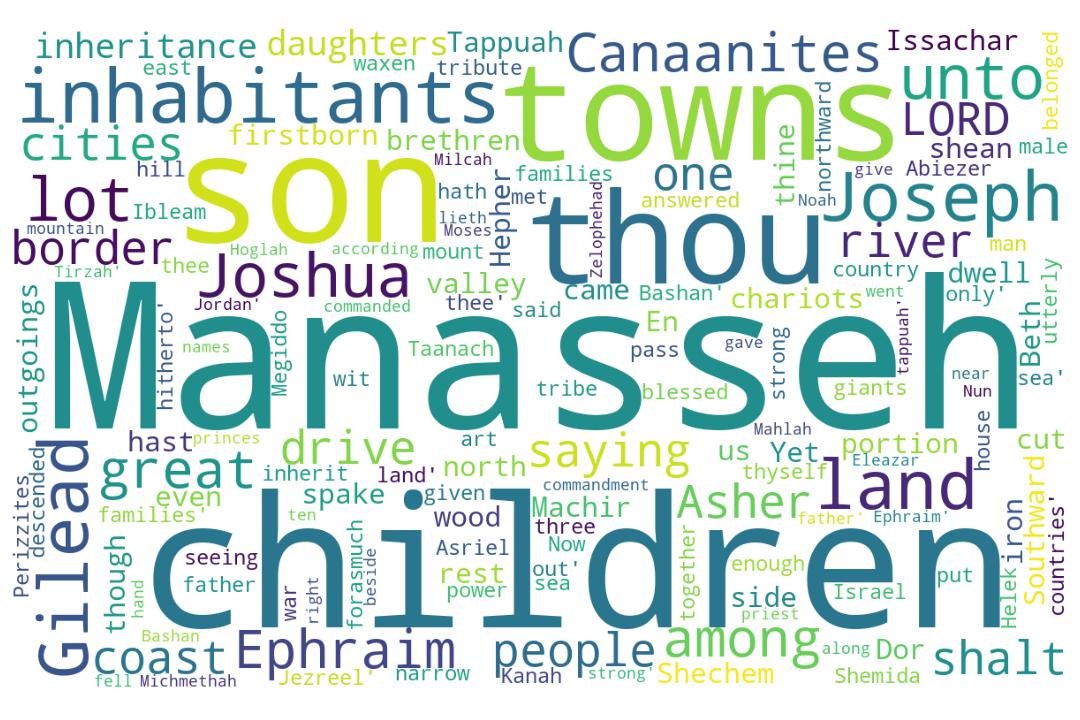
\includegraphics[width=\linewidth]{06OT-Joshua/Joshua17-WordCloud.jpg}
  \caption{Joshua 17 Word Cloud}
  \label{fig:Joshua 17 Word Cloud}
\end{figure}

\marginpar{\scriptsize \centering \fcolorbox{bone}{lime}{\textbf{MANASSEH ON THE WEST SIDE}}\\ (Joshua 17:1-18) \begin{compactenum}[I.][8]
	\item The \textbf{Daughters}  \index[scripture]{Joshua!Jsh 16:03}\index[scripture]{Joshua!Jsh 17:06}  (Jsh 17:3, 6) 
	\item The \textbf{Decree}  \index[scripture]{Joshua!Jsh 16:04}  (Joshua 17:4) (so what happens when the male line to the throne is cut off? This decree determines that Mary's descendant has a right to the throne
	\item The \textbf{Descendants} (the word ``children'' found 13 times in the chapter\index[scripture]{Joshua!Jsh 16:02}  \index[scripture]{Joshua!Jsh 17:08}  \index[scripture]{Joshua!Jsh 17:13}  \index[scripture]{Joshua!Jsh 17:14}  \index[scripture]{Joshua!Jsh 17:16}  (Jsh 17:2 (8x), 8, 12, 13, 14, 16) 
	\item The \textbf{Dwellers}  \index[scripture]{Joshua!Jsh 17:12}\index[scripture]{Joshua!Jsh 17:16}   (Joshua Jsh:12, 16) 
	\item \textbf{Drive} out the Canaanites \index[scripture]{Joshua!Jsh 17:12}\index[scripture]{Joshua!Jsh 17:13} \index[scripture]{Joshua!Jsh 17:18}  (Jsh 17:12, 13, 18) 
	\item We're \textbf{Disdavantaged}  \index[scripture]{Joshua!Jsh 17:12}\index[scripture]{Joshua!Jsh 17:16}   (Jsh 17:16) 
	\item Joshua's \textbf{Determination}  \index[scripture]{Joshua!Jsh 17:18} (Jsh 17:18) 
\end{compactenum}}






\footnote{\textcolor[cmyk]{0.99998,1,0,0}{\hyperlink{TOC}{Return to end of Table of Contents.}}}\footnote{\href{https://audiobible.com/bible/joshua_17.html}{\textcolor[cmyk]{0.99998,1,0,0}{Joshua 17 Audio}}}\textcolor[cmyk]{0.99998,1,0,0}{There was also a lot for the tribe of Manasseh; for he \emph{was} the firstborn of Joseph; \emph{to} \emph{wit}, for Machir the firstborn of Manasseh, the father of Gilead: because he was a man of war, therefore he had Gilead and Bashan.}
[2] \textcolor[cmyk]{0.99998,1,0,0}{There was also \emph{a} \emph{lot} for the rest of the \fcolorbox{bone}{bone}{children of} Manasseh by their families; for the \fcolorbox{bone}{bone}{children of} Abiezer, and for the \fcolorbox{bone}{bone}{children of} Helek, and for the \fcolorbox{bone}{bone}{children of} Asriel, and for the \fcolorbox{bone}{bone}{children of} Shechem, and for the \fcolorbox{bone}{bone}{children of} Hepher, and for the \fcolorbox{bone}{bone}{children of} Shemida: these \emph{were} the male \fcolorbox{bone}{bone}{children of} Manasseh the son of Joseph by their families.}\\
\\
\P \textcolor[cmyk]{0.99998,1,0,0}{But Zelophehad, the son of Hepher, the son of Gilead, the son of Machir, the son of Manasseh, had no sons, but daughters: and these \emph{are} the names of his daughters, \fcolorbox{bone}{lime}{Mahlah}, and \fcolorbox{bone}{lime}{Noah}, \fcolorbox{bone}{lime}{Hoglah}, \fcolorbox{bone}{lime}{Milcah}, and \fcolorbox{bone}{lime}{Trzah}.}
[4] \textcolor[cmyk]{0.99998,1,0,0}{And they came near before Eleazar the priest, and before Joshua the son of Nun, and before the princes, saying, The LORD commanded Moses to give us an inheritance among our brethren. Therefore according to the \fcolorbox{bone}{lime}{commandment} of the LORD he gave them an inheritance among the brethren of their father.}
[5] \textcolor[cmyk]{0.99998,1,0,0}{And there fell ten portions to Manasseh, beside the land of Gilead and Bashan, which \emph{were} on the other side Jordan;}
[6] \textcolor[cmyk]{0.99998,1,0,0}{Because the daughters of Manasseh had an inheritance among his sons: and the rest of Manasseh's sons had the land of Gilead.}\\
\\
\P \textcolor[cmyk]{0.99998,1,0,0}{And the coast of Manasseh was from Asher to Michmethah, that \emph{lieth} before Shechem; and the border went along on the right hand unto the inhabitants of En-tappuah.}
[8] \textcolor[cmyk]{0.99998,1,0,0}{\emph{Now} Manasseh had the land of Tappuah: but Tappuah on the border of Manasseh \emph{belonged} to the \fcolorbox{bone}{bone}{children of} Ephraim;}
[9] \textcolor[cmyk]{0.99998,1,0,0}{And the coast descended unto the river Kanah, southward of the river: these cities of Ephraim \emph{are} among the cities of Manasseh: the coast of Manasseh also \emph{was} on the north side of the river, and the outgoings of it were at the sea:}
[10] \textcolor[cmyk]{0.99998,1,0,0}{Southward \emph{it} \emph{was} Ephraim's, and northward \emph{it} \emph{was} Manasseh's, and the sea is his border; and they met together in Asher on the north, and in Issachar on the east.}
[11] \textcolor[cmyk]{0.99998,1,0,0}{And Manasseh had in Issachar and in Asher Beth-shean and her towns, and Ibleam and her towns, and the inhabitants of Dor and her towns, and the inhabitants of En-dor and her towns, and the inhabitants of Taanach and her towns, and the inhabitants of Megiddo and her towns, \emph{even} three countries.}
[12] \textcolor[cmyk]{0.99998,1,0,0}{Yet the \fcolorbox{bone}{bone}{children of} Manasseh could not \fcolorbox{bone}{lime}{drive out} \emph{the} \emph{inhabitants} \emph{of} those cities; but the Canaanites would \fcolorbox{bone}{lime}{dwell} in that land.}
[13] \textcolor[cmyk]{0.99998,1,0,0}{Yet it came to pass, when the \fcolorbox{bone}{bone}{children of} Israel were waxen strong, that they put the Canaanites to tribute; but did not utterly drive them out.}
[14] \textcolor[cmyk]{0.99998,1,0,0}{And the \fcolorbox{bone}{bone}{children of} Joseph spake unto Joshua, saying, Why hast thou given me \emph{but} one lot and one portion to inherit, seeing I \emph{am} a great people, forasmuch as the LORD hath blessed me hitherto?}
[15] \textcolor[cmyk]{0.99998,1,0,0}{And Joshua answered them, If thou \emph{be} a great people, \emph{then} get thee up to the wood \emph{country}, and cut down for thyself there in the land of the Perizzites and of the giants, if mount Ephraim be too narrow for thee.}
[16] \textcolor[cmyk]{0.99998,1,0,0}{And the \fcolorbox{bone}{bone}{children of} Joseph said, The hill is \fcolorbox{bone}{lime}{not enough} for us: and all the Canaanites that dwell in the land of the valley have chariots of iron, \emph{both} \emph{they} who \emph{are} of Beth-shean and her towns, and \emph{they} who \emph{are} of the valley of Jezreel.}
[17] \textcolor[cmyk]{0.99998,1,0,0}{And Joshua spake unto the house of Joseph, \emph{even} to Ephraim and to Manasseh, saying, Thou \emph{art} a great people, and hast great power: thou shalt not have one lot \emph{only}:}
[18] \textcolor[cmyk]{0.99998,1,0,0}{But the mountain shall be thine; for it \emph{is} a wood, and thou shalt cut it down: and the outgoings of it shall be thine: for \fcolorbox{bone}{lime}{thou shalt} drive out the Canaanites, though they have iron chariots, \emph{and} though they \emph{be} strong.}
\index[NWIV]{42!Joshua!Jos 17:1}\index[AWIP]{There!Joshua!Jos 17:1}\index[AWIP]{was!Joshua!Jos 17:1}\index[AWIP]{was!Joshua!Jos 17:1 (2)}\index[AWIP]{also!Joshua!Jos 17:1}\index[AWIP]{a!Joshua!Jos 17:1}\index[AWIP]{a!Joshua!Jos 17:1 (2)}\index[AWIP]{lot!Joshua!Jos 17:1}\index[AWIP]{for!Joshua!Jos 17:1}\index[AWIP]{for!Joshua!Jos 17:1 (2)}\index[AWIP]{for!Joshua!Jos 17:1 (3)}\index[AWIP]{the!Joshua!Jos 17:1}\index[AWIP]{the!Joshua!Jos 17:1 (2)}\index[AWIP]{the!Joshua!Jos 17:1 (3)}\index[AWIP]{the!Joshua!Jos 17:1 (4)}\index[AWIP]{tribe!Joshua!Jos 17:1}\index[AWIP]{of!Joshua!Jos 17:1}\index[AWIP]{of!Joshua!Jos 17:1 (2)}\index[AWIP]{of!Joshua!Jos 17:1 (3)}\index[AWIP]{of!Joshua!Jos 17:1 (4)}\index[AWIP]{of!Joshua!Jos 17:1 (5)}\index[AWIP]{Manasseh!Joshua!Jos 17:1}\index[AWIP]{Manasseh!Joshua!Jos 17:1 (2)}\index[AWIP]{he!Joshua!Jos 17:1}\index[AWIP]{he!Joshua!Jos 17:1 (2)}\index[AWIP]{he!Joshua!Jos 17:1 (3)}\index[AWIP]{\emph{was}!Joshua!Jos 17:1}\index[AWIP]{firstborn!Joshua!Jos 17:1}\index[AWIP]{firstborn!Joshua!Jos 17:1 (2)}\index[AWIP]{Joseph!Joshua!Jos 17:1}\index[AWIP]{\emph{to}!Joshua!Jos 17:1}\index[AWIP]{\emph{wit}!Joshua!Jos 17:1}\index[AWIP]{Machir!Joshua!Jos 17:1}\index[AWIP]{father!Joshua!Jos 17:1}\index[AWIP]{Gilead!Joshua!Jos 17:1}\index[AWIP]{Gilead!Joshua!Jos 17:1 (2)}\index[AWIP]{because!Joshua!Jos 17:1}\index[AWIP]{man!Joshua!Jos 17:1}\index[AWIP]{war!Joshua!Jos 17:1}\index[AWIP]{therefore!Joshua!Jos 17:1}\index[AWIP]{had!Joshua!Jos 17:1}\index[AWIP]{and!Joshua!Jos 17:1}\index[AWIP]{Bashan!Joshua!Jos 17:1}\index[AWIP]{\emph{was}!Joshua!Jos 17:1}\index[AWIP]{\emph{to}!Joshua!Jos 17:1}\index[AWIP]{\emph{wit}!Joshua!Jos 17:1}

\index[NWIV]{65!Joshua!Jos 17:2}\index[AWIP]{There!Joshua!Jos 17:2}\index[AWIP]{was!Joshua!Jos 17:2}\index[AWIP]{also!Joshua!Jos 17:2}\index[AWIP]{\emph{a}!Joshua!Jos 17:2}\index[AWIP]{\emph{lot}!Joshua!Jos 17:2}\index[AWIP]{for!Joshua!Jos 17:2}\index[AWIP]{for!Joshua!Jos 17:2 (2)}\index[AWIP]{for!Joshua!Jos 17:2 (3)}\index[AWIP]{for!Joshua!Jos 17:2 (4)}\index[AWIP]{for!Joshua!Jos 17:2 (5)}\index[AWIP]{for!Joshua!Jos 17:2 (6)}\index[AWIP]{for!Joshua!Jos 17:2 (7)}\index[AWIP]{the!Joshua!Jos 17:2}\index[AWIP]{the!Joshua!Jos 17:2 (2)}\index[AWIP]{the!Joshua!Jos 17:2 (3)}\index[AWIP]{the!Joshua!Jos 17:2 (4)}\index[AWIP]{the!Joshua!Jos 17:2 (5)}\index[AWIP]{the!Joshua!Jos 17:2 (6)}\index[AWIP]{the!Joshua!Jos 17:2 (7)}\index[AWIP]{the!Joshua!Jos 17:2 (8)}\index[AWIP]{the!Joshua!Jos 17:2 (9)}\index[AWIP]{the!Joshua!Jos 17:2 (10)}\index[AWIP]{rest!Joshua!Jos 17:2}\index[AWIP]{of!Joshua!Jos 17:2}\index[AWIP]{of!Joshua!Jos 17:2 (2)}\index[AWIP]{of!Joshua!Jos 17:2 (3)}\index[AWIP]{of!Joshua!Jos 17:2 (4)}\index[AWIP]{of!Joshua!Jos 17:2 (5)}\index[AWIP]{of!Joshua!Jos 17:2 (6)}\index[AWIP]{of!Joshua!Jos 17:2 (7)}\index[AWIP]{of!Joshua!Jos 17:2 (8)}\index[AWIP]{of!Joshua!Jos 17:2 (9)}\index[AWIP]{of!Joshua!Jos 17:2 (10)}\index[AWIP]{children!Joshua!Jos 17:2}\index[AWIP]{children!Joshua!Jos 17:2 (2)}\index[AWIP]{children!Joshua!Jos 17:2 (3)}\index[AWIP]{children!Joshua!Jos 17:2 (4)}\index[AWIP]{children!Joshua!Jos 17:2 (5)}\index[AWIP]{children!Joshua!Jos 17:2 (6)}\index[AWIP]{children!Joshua!Jos 17:2 (7)}\index[AWIP]{children!Joshua!Jos 17:2 (8)}\index[AWIP]{Manasseh!Joshua!Jos 17:2}\index[AWIP]{Manasseh!Joshua!Jos 17:2 (2)}\index[AWIP]{by!Joshua!Jos 17:2}\index[AWIP]{by!Joshua!Jos 17:2 (2)}\index[AWIP]{their!Joshua!Jos 17:2}\index[AWIP]{their!Joshua!Jos 17:2 (2)}\index[AWIP]{families!Joshua!Jos 17:2}\index[AWIP]{families!Joshua!Jos 17:2 (2)}\index[AWIP]{Abiezer!Joshua!Jos 17:2}\index[AWIP]{and!Joshua!Jos 17:2}\index[AWIP]{and!Joshua!Jos 17:2 (2)}\index[AWIP]{and!Joshua!Jos 17:2 (3)}\index[AWIP]{and!Joshua!Jos 17:2 (4)}\index[AWIP]{and!Joshua!Jos 17:2 (5)}\index[AWIP]{Helek!Joshua!Jos 17:2}\index[AWIP]{Asriel!Joshua!Jos 17:2}\index[AWIP]{Shechem!Joshua!Jos 17:2}\index[AWIP]{Hepher!Joshua!Jos 17:2}\index[AWIP]{Shemida!Joshua!Jos 17:2}\index[AWIP]{these!Joshua!Jos 17:2}\index[AWIP]{\emph{were}!Joshua!Jos 17:2}\index[AWIP]{male!Joshua!Jos 17:2}\index[AWIP]{son!Joshua!Jos 17:2}\index[AWIP]{Joseph!Joshua!Jos 17:2}\index[AWIP]{\emph{a}!Joshua!Jos 17:2}\index[AWIP]{\emph{lot}!Joshua!Jos 17:2}\index[AWIP]{\emph{were}!Joshua!Jos 17:2}

\index[NWIV]{38!Joshua!Jos 17:3}\index[AWIP]{But!Joshua!Jos 17:3}\index[AWIP]{Zelophehad!Joshua!Jos 17:3}\index[AWIP]{the!Joshua!Jos 17:3}\index[AWIP]{the!Joshua!Jos 17:3 (2)}\index[AWIP]{the!Joshua!Jos 17:3 (3)}\index[AWIP]{the!Joshua!Jos 17:3 (4)}\index[AWIP]{the!Joshua!Jos 17:3 (5)}\index[AWIP]{son!Joshua!Jos 17:3}\index[AWIP]{son!Joshua!Jos 17:3 (2)}\index[AWIP]{son!Joshua!Jos 17:3 (3)}\index[AWIP]{son!Joshua!Jos 17:3 (4)}\index[AWIP]{of!Joshua!Jos 17:3}\index[AWIP]{of!Joshua!Jos 17:3 (2)}\index[AWIP]{of!Joshua!Jos 17:3 (3)}\index[AWIP]{of!Joshua!Jos 17:3 (4)}\index[AWIP]{of!Joshua!Jos 17:3 (5)}\index[AWIP]{Hepher!Joshua!Jos 17:3}\index[AWIP]{Gilead!Joshua!Jos 17:3}\index[AWIP]{Machir!Joshua!Jos 17:3}\index[AWIP]{Manasseh!Joshua!Jos 17:3}\index[AWIP]{had!Joshua!Jos 17:3}\index[AWIP]{no!Joshua!Jos 17:3}\index[AWIP]{sons!Joshua!Jos 17:3}\index[AWIP]{but!Joshua!Jos 17:3}\index[AWIP]{daughters!Joshua!Jos 17:3}\index[AWIP]{daughters!Joshua!Jos 17:3 (2)}\index[AWIP]{and!Joshua!Jos 17:3}\index[AWIP]{and!Joshua!Jos 17:3 (2)}\index[AWIP]{and!Joshua!Jos 17:3 (3)}\index[AWIP]{these!Joshua!Jos 17:3}\index[AWIP]{\emph{are}!Joshua!Jos 17:3}\index[AWIP]{names!Joshua!Jos 17:3}\index[AWIP]{his!Joshua!Jos 17:3}\index[AWIP]{Mahlah!Joshua!Jos 17:3}\index[AWIP]{Noah!Joshua!Jos 17:3}\index[AWIP]{Hoglah!Joshua!Jos 17:3}\index[AWIP]{Milcah!Joshua!Jos 17:3}\index[AWIP]{Tirzah!Joshua!Jos 17:3}\index[AWIP]{\emph{are}!Joshua!Jos 17:3}

\index[NWIV]{51!Joshua!Jos 17:4}\index[AWIP]{And!Joshua!Jos 17:4}\index[AWIP]{they!Joshua!Jos 17:4}\index[AWIP]{came!Joshua!Jos 17:4}\index[AWIP]{near!Joshua!Jos 17:4}\index[AWIP]{before!Joshua!Jos 17:4}\index[AWIP]{before!Joshua!Jos 17:4 (2)}\index[AWIP]{before!Joshua!Jos 17:4 (3)}\index[AWIP]{Eleazar!Joshua!Jos 17:4}\index[AWIP]{the!Joshua!Jos 17:4}\index[AWIP]{the!Joshua!Jos 17:4 (2)}\index[AWIP]{the!Joshua!Jos 17:4 (3)}\index[AWIP]{the!Joshua!Jos 17:4 (4)}\index[AWIP]{the!Joshua!Jos 17:4 (5)}\index[AWIP]{the!Joshua!Jos 17:4 (6)}\index[AWIP]{priest!Joshua!Jos 17:4}\index[AWIP]{and!Joshua!Jos 17:4}\index[AWIP]{and!Joshua!Jos 17:4 (2)}\index[AWIP]{Joshua!Joshua!Jos 17:4}\index[AWIP]{son!Joshua!Jos 17:4}\index[AWIP]{of!Joshua!Jos 17:4}\index[AWIP]{of!Joshua!Jos 17:4 (2)}\index[AWIP]{of!Joshua!Jos 17:4 (3)}\index[AWIP]{Nun!Joshua!Jos 17:4}\index[AWIP]{princes!Joshua!Jos 17:4}\index[AWIP]{saying!Joshua!Jos 17:4}\index[AWIP]{The!Joshua!Jos 17:4}\index[AWIP]{LORD!Joshua!Jos 17:4}\index[AWIP]{LORD!Joshua!Jos 17:4 (2)}\index[AWIP]{commanded!Joshua!Jos 17:4}\index[AWIP]{Moses!Joshua!Jos 17:4}\index[AWIP]{to!Joshua!Jos 17:4}\index[AWIP]{to!Joshua!Jos 17:4 (2)}\index[AWIP]{give!Joshua!Jos 17:4}\index[AWIP]{us!Joshua!Jos 17:4}\index[AWIP]{an!Joshua!Jos 17:4}\index[AWIP]{an!Joshua!Jos 17:4 (2)}\index[AWIP]{inheritance!Joshua!Jos 17:4}\index[AWIP]{inheritance!Joshua!Jos 17:4 (2)}\index[AWIP]{among!Joshua!Jos 17:4}\index[AWIP]{among!Joshua!Jos 17:4 (2)}\index[AWIP]{our!Joshua!Jos 17:4}\index[AWIP]{brethren!Joshua!Jos 17:4}\index[AWIP]{brethren!Joshua!Jos 17:4 (2)}\index[AWIP]{Therefore!Joshua!Jos 17:4}\index[AWIP]{according!Joshua!Jos 17:4}\index[AWIP]{commandment!Joshua!Jos 17:4}\index[AWIP]{he!Joshua!Jos 17:4}\index[AWIP]{gave!Joshua!Jos 17:4}\index[AWIP]{them!Joshua!Jos 17:4}\index[AWIP]{their!Joshua!Jos 17:4}\index[AWIP]{father!Joshua!Jos 17:4}

\index[NWIV]{21!Joshua!Jos 17:5}\index[AWIP]{And!Joshua!Jos 17:5}\index[AWIP]{there!Joshua!Jos 17:5}\index[AWIP]{fell!Joshua!Jos 17:5}\index[AWIP]{ten!Joshua!Jos 17:5}\index[AWIP]{portions!Joshua!Jos 17:5}\index[AWIP]{to!Joshua!Jos 17:5}\index[AWIP]{Manasseh!Joshua!Jos 17:5}\index[AWIP]{beside!Joshua!Jos 17:5}\index[AWIP]{the!Joshua!Jos 17:5}\index[AWIP]{the!Joshua!Jos 17:5 (2)}\index[AWIP]{land!Joshua!Jos 17:5}\index[AWIP]{of!Joshua!Jos 17:5}\index[AWIP]{Gilead!Joshua!Jos 17:5}\index[AWIP]{and!Joshua!Jos 17:5}\index[AWIP]{Bashan!Joshua!Jos 17:5}\index[AWIP]{which!Joshua!Jos 17:5}\index[AWIP]{\emph{were}!Joshua!Jos 17:5}\index[AWIP]{on!Joshua!Jos 17:5}\index[AWIP]{other!Joshua!Jos 17:5}\index[AWIP]{side!Joshua!Jos 17:5}\index[AWIP]{Jordan!Joshua!Jos 17:5}\index[AWIP]{\emph{were}!Joshua!Jos 17:5}

\index[NWIV]{22!Joshua!Jos 17:6}\index[AWIP]{Because!Joshua!Jos 17:6}\index[AWIP]{the!Joshua!Jos 17:6}\index[AWIP]{the!Joshua!Jos 17:6 (2)}\index[AWIP]{the!Joshua!Jos 17:6 (3)}\index[AWIP]{daughters!Joshua!Jos 17:6}\index[AWIP]{of!Joshua!Jos 17:6}\index[AWIP]{of!Joshua!Jos 17:6 (2)}\index[AWIP]{of!Joshua!Jos 17:6 (3)}\index[AWIP]{Manasseh!Joshua!Jos 17:6}\index[AWIP]{had!Joshua!Jos 17:6}\index[AWIP]{had!Joshua!Jos 17:6 (2)}\index[AWIP]{an!Joshua!Jos 17:6}\index[AWIP]{inheritance!Joshua!Jos 17:6}\index[AWIP]{among!Joshua!Jos 17:6}\index[AWIP]{his!Joshua!Jos 17:6}\index[AWIP]{sons!Joshua!Jos 17:6}\index[AWIP]{sons!Joshua!Jos 17:6 (2)}\index[AWIP]{and!Joshua!Jos 17:6}\index[AWIP]{rest!Joshua!Jos 17:6}\index[AWIP]{Manasseh's!Joshua!Jos 17:6}\index[AWIP]{land!Joshua!Jos 17:6}\index[AWIP]{Gilead!Joshua!Jos 17:6}

\index[NWIV]{28!Joshua!Jos 17:7}\index[AWIP]{And!Joshua!Jos 17:7}\index[AWIP]{the!Joshua!Jos 17:7}\index[AWIP]{the!Joshua!Jos 17:7 (2)}\index[AWIP]{the!Joshua!Jos 17:7 (3)}\index[AWIP]{the!Joshua!Jos 17:7 (4)}\index[AWIP]{coast!Joshua!Jos 17:7}\index[AWIP]{of!Joshua!Jos 17:7}\index[AWIP]{of!Joshua!Jos 17:7 (2)}\index[AWIP]{Manasseh!Joshua!Jos 17:7}\index[AWIP]{was!Joshua!Jos 17:7}\index[AWIP]{from!Joshua!Jos 17:7}\index[AWIP]{Asher!Joshua!Jos 17:7}\index[AWIP]{to!Joshua!Jos 17:7}\index[AWIP]{Michmethah!Joshua!Jos 17:7}\index[AWIP]{that!Joshua!Jos 17:7}\index[AWIP]{\emph{lieth}!Joshua!Jos 17:7}\index[AWIP]{before!Joshua!Jos 17:7}\index[AWIP]{Shechem!Joshua!Jos 17:7}\index[AWIP]{and!Joshua!Jos 17:7}\index[AWIP]{border!Joshua!Jos 17:7}\index[AWIP]{went!Joshua!Jos 17:7}\index[AWIP]{along!Joshua!Jos 17:7}\index[AWIP]{on!Joshua!Jos 17:7}\index[AWIP]{right!Joshua!Jos 17:7}\index[AWIP]{hand!Joshua!Jos 17:7}\index[AWIP]{unto!Joshua!Jos 17:7}\index[AWIP]{inhabitants!Joshua!Jos 17:7}\index[AWIP]{En-tappuah!Joshua!Jos 17:7}\index[AWIP]{\emph{lieth}!Joshua!Jos 17:7}

\index[NWIV]{20!Joshua!Jos 17:8}\index[AWIP]{\emph{Now}!Joshua!Jos 17:8}\index[AWIP]{Manasseh!Joshua!Jos 17:8}\index[AWIP]{Manasseh!Joshua!Jos 17:8 (2)}\index[AWIP]{had!Joshua!Jos 17:8}\index[AWIP]{the!Joshua!Jos 17:8}\index[AWIP]{the!Joshua!Jos 17:8 (2)}\index[AWIP]{the!Joshua!Jos 17:8 (3)}\index[AWIP]{land!Joshua!Jos 17:8}\index[AWIP]{of!Joshua!Jos 17:8}\index[AWIP]{of!Joshua!Jos 17:8 (2)}\index[AWIP]{of!Joshua!Jos 17:8 (3)}\index[AWIP]{Tappuah!Joshua!Jos 17:8}\index[AWIP]{Tappuah!Joshua!Jos 17:8 (2)}\index[AWIP]{but!Joshua!Jos 17:8}\index[AWIP]{on!Joshua!Jos 17:8}\index[AWIP]{border!Joshua!Jos 17:8}\index[AWIP]{\emph{belonged}!Joshua!Jos 17:8}\index[AWIP]{to!Joshua!Jos 17:8}\index[AWIP]{children!Joshua!Jos 17:8}\index[AWIP]{Ephraim!Joshua!Jos 17:8}\index[AWIP]{\emph{Now}!Joshua!Jos 17:8}\index[AWIP]{\emph{belonged}!Joshua!Jos 17:8}

\index[NWIV]{44!Joshua!Jos 17:9}\index[AWIP]{And!Joshua!Jos 17:9}\index[AWIP]{the!Joshua!Jos 17:9}\index[AWIP]{the!Joshua!Jos 17:9 (2)}\index[AWIP]{the!Joshua!Jos 17:9 (3)}\index[AWIP]{the!Joshua!Jos 17:9 (4)}\index[AWIP]{the!Joshua!Jos 17:9 (5)}\index[AWIP]{the!Joshua!Jos 17:9 (6)}\index[AWIP]{the!Joshua!Jos 17:9 (7)}\index[AWIP]{the!Joshua!Jos 17:9 (8)}\index[AWIP]{the!Joshua!Jos 17:9 (9)}\index[AWIP]{coast!Joshua!Jos 17:9}\index[AWIP]{coast!Joshua!Jos 17:9 (2)}\index[AWIP]{descended!Joshua!Jos 17:9}\index[AWIP]{unto!Joshua!Jos 17:9}\index[AWIP]{river!Joshua!Jos 17:9}\index[AWIP]{river!Joshua!Jos 17:9 (2)}\index[AWIP]{river!Joshua!Jos 17:9 (3)}\index[AWIP]{Kanah!Joshua!Jos 17:9}\index[AWIP]{southward!Joshua!Jos 17:9}\index[AWIP]{of!Joshua!Jos 17:9}\index[AWIP]{of!Joshua!Jos 17:9 (2)}\index[AWIP]{of!Joshua!Jos 17:9 (3)}\index[AWIP]{of!Joshua!Jos 17:9 (4)}\index[AWIP]{of!Joshua!Jos 17:9 (5)}\index[AWIP]{of!Joshua!Jos 17:9 (6)}\index[AWIP]{these!Joshua!Jos 17:9}\index[AWIP]{cities!Joshua!Jos 17:9}\index[AWIP]{cities!Joshua!Jos 17:9 (2)}\index[AWIP]{Ephraim!Joshua!Jos 17:9}\index[AWIP]{\emph{are}!Joshua!Jos 17:9}\index[AWIP]{among!Joshua!Jos 17:9}\index[AWIP]{Manasseh!Joshua!Jos 17:9}\index[AWIP]{Manasseh!Joshua!Jos 17:9 (2)}\index[AWIP]{also!Joshua!Jos 17:9}\index[AWIP]{\emph{was}!Joshua!Jos 17:9}\index[AWIP]{on!Joshua!Jos 17:9}\index[AWIP]{north!Joshua!Jos 17:9}\index[AWIP]{side!Joshua!Jos 17:9}\index[AWIP]{and!Joshua!Jos 17:9}\index[AWIP]{outgoings!Joshua!Jos 17:9}\index[AWIP]{it!Joshua!Jos 17:9}\index[AWIP]{were!Joshua!Jos 17:9}\index[AWIP]{at!Joshua!Jos 17:9}\index[AWIP]{sea!Joshua!Jos 17:9}\index[AWIP]{\emph{are}!Joshua!Jos 17:9}\index[AWIP]{\emph{was}!Joshua!Jos 17:9}

\index[NWIV]{30!Joshua!Jos 17:10}\index[AWIP]{Southward!Joshua!Jos 17:10}\index[AWIP]{\emph{it}!Joshua!Jos 17:10}\index[AWIP]{\emph{it}!Joshua!Jos 17:10 (2)}\index[AWIP]{\emph{was}!Joshua!Jos 17:10}\index[AWIP]{\emph{was}!Joshua!Jos 17:10 (2)}\index[AWIP]{Ephraim's!Joshua!Jos 17:10}\index[AWIP]{and!Joshua!Jos 17:10}\index[AWIP]{and!Joshua!Jos 17:10 (2)}\index[AWIP]{and!Joshua!Jos 17:10 (3)}\index[AWIP]{and!Joshua!Jos 17:10 (4)}\index[AWIP]{northward!Joshua!Jos 17:10}\index[AWIP]{Manasseh's!Joshua!Jos 17:10}\index[AWIP]{the!Joshua!Jos 17:10}\index[AWIP]{the!Joshua!Jos 17:10 (2)}\index[AWIP]{the!Joshua!Jos 17:10 (3)}\index[AWIP]{sea!Joshua!Jos 17:10}\index[AWIP]{is!Joshua!Jos 17:10}\index[AWIP]{his!Joshua!Jos 17:10}\index[AWIP]{border!Joshua!Jos 17:10}\index[AWIP]{they!Joshua!Jos 17:10}\index[AWIP]{met!Joshua!Jos 17:10}\index[AWIP]{together!Joshua!Jos 17:10}\index[AWIP]{in!Joshua!Jos 17:10}\index[AWIP]{in!Joshua!Jos 17:10 (2)}\index[AWIP]{Asher!Joshua!Jos 17:10}\index[AWIP]{on!Joshua!Jos 17:10}\index[AWIP]{on!Joshua!Jos 17:10 (2)}\index[AWIP]{north!Joshua!Jos 17:10}\index[AWIP]{Issachar!Joshua!Jos 17:10}\index[AWIP]{east!Joshua!Jos 17:10}\index[AWIP]{\emph{it}!Joshua!Jos 17:10}\index[AWIP]{\emph{it}!Joshua!Jos 17:10 (2)}\index[AWIP]{\emph{was}!Joshua!Jos 17:10}\index[AWIP]{\emph{was}!Joshua!Jos 17:10 (2)}

\index[NWIV]{52!Joshua!Jos 17:11}\index[AWIP]{And!Joshua!Jos 17:11}\index[AWIP]{Manasseh!Joshua!Jos 17:11}\index[AWIP]{had!Joshua!Jos 17:11}\index[AWIP]{in!Joshua!Jos 17:11}\index[AWIP]{in!Joshua!Jos 17:11 (2)}\index[AWIP]{Issachar!Joshua!Jos 17:11}\index[AWIP]{and!Joshua!Jos 17:11}\index[AWIP]{and!Joshua!Jos 17:11 (2)}\index[AWIP]{and!Joshua!Jos 17:11 (3)}\index[AWIP]{and!Joshua!Jos 17:11 (4)}\index[AWIP]{and!Joshua!Jos 17:11 (5)}\index[AWIP]{and!Joshua!Jos 17:11 (6)}\index[AWIP]{and!Joshua!Jos 17:11 (7)}\index[AWIP]{and!Joshua!Jos 17:11 (8)}\index[AWIP]{and!Joshua!Jos 17:11 (9)}\index[AWIP]{and!Joshua!Jos 17:11 (10)}\index[AWIP]{and!Joshua!Jos 17:11 (11)}\index[AWIP]{and!Joshua!Jos 17:11 (12)}\index[AWIP]{Asher!Joshua!Jos 17:11}\index[AWIP]{Beth-shean!Joshua!Jos 17:11}\index[AWIP]{her!Joshua!Jos 17:11}\index[AWIP]{her!Joshua!Jos 17:11 (2)}\index[AWIP]{her!Joshua!Jos 17:11 (3)}\index[AWIP]{her!Joshua!Jos 17:11 (4)}\index[AWIP]{her!Joshua!Jos 17:11 (5)}\index[AWIP]{her!Joshua!Jos 17:11 (6)}\index[AWIP]{towns!Joshua!Jos 17:11}\index[AWIP]{towns!Joshua!Jos 17:11 (2)}\index[AWIP]{towns!Joshua!Jos 17:11 (3)}\index[AWIP]{towns!Joshua!Jos 17:11 (4)}\index[AWIP]{towns!Joshua!Jos 17:11 (5)}\index[AWIP]{towns!Joshua!Jos 17:11 (6)}\index[AWIP]{Ibleam!Joshua!Jos 17:11}\index[AWIP]{the!Joshua!Jos 17:11}\index[AWIP]{the!Joshua!Jos 17:11 (2)}\index[AWIP]{the!Joshua!Jos 17:11 (3)}\index[AWIP]{the!Joshua!Jos 17:11 (4)}\index[AWIP]{inhabitants!Joshua!Jos 17:11}\index[AWIP]{inhabitants!Joshua!Jos 17:11 (2)}\index[AWIP]{inhabitants!Joshua!Jos 17:11 (3)}\index[AWIP]{inhabitants!Joshua!Jos 17:11 (4)}\index[AWIP]{of!Joshua!Jos 17:11}\index[AWIP]{of!Joshua!Jos 17:11 (2)}\index[AWIP]{of!Joshua!Jos 17:11 (3)}\index[AWIP]{of!Joshua!Jos 17:11 (4)}\index[AWIP]{Dor!Joshua!Jos 17:11}\index[AWIP]{En-dor!Joshua!Jos 17:11}\index[AWIP]{Taanach!Joshua!Jos 17:11}\index[AWIP]{Megiddo!Joshua!Jos 17:11}\index[AWIP]{\emph{even}!Joshua!Jos 17:11}\index[AWIP]{three!Joshua!Jos 17:11}\index[AWIP]{countries!Joshua!Jos 17:11}\index[AWIP]{\emph{even}!Joshua!Jos 17:11}

\index[NWIV]{22!Joshua!Jos 17:12}\index[AWIP]{Yet!Joshua!Jos 17:12}\index[AWIP]{the!Joshua!Jos 17:12}\index[AWIP]{the!Joshua!Jos 17:12 (2)}\index[AWIP]{children!Joshua!Jos 17:12}\index[AWIP]{of!Joshua!Jos 17:12}\index[AWIP]{Manasseh!Joshua!Jos 17:12}\index[AWIP]{could!Joshua!Jos 17:12}\index[AWIP]{not!Joshua!Jos 17:12}\index[AWIP]{drive!Joshua!Jos 17:12}\index[AWIP]{out!Joshua!Jos 17:12}\index[AWIP]{\emph{the}!Joshua!Jos 17:12}\index[AWIP]{\emph{inhabitants}!Joshua!Jos 17:12}\index[AWIP]{\emph{of}!Joshua!Jos 17:12}\index[AWIP]{those!Joshua!Jos 17:12}\index[AWIP]{cities!Joshua!Jos 17:12}\index[AWIP]{but!Joshua!Jos 17:12}\index[AWIP]{Canaanites!Joshua!Jos 17:12}\index[AWIP]{would!Joshua!Jos 17:12}\index[AWIP]{dwell!Joshua!Jos 17:12}\index[AWIP]{in!Joshua!Jos 17:12}\index[AWIP]{that!Joshua!Jos 17:12}\index[AWIP]{land!Joshua!Jos 17:12}\index[AWIP]{\emph{the}!Joshua!Jos 17:12}\index[AWIP]{\emph{inhabitants}!Joshua!Jos 17:12}\index[AWIP]{\emph{of}!Joshua!Jos 17:12}

\index[NWIV]{27!Joshua!Jos 17:13}\index[AWIP]{Yet!Joshua!Jos 17:13}\index[AWIP]{it!Joshua!Jos 17:13}\index[AWIP]{came!Joshua!Jos 17:13}\index[AWIP]{to!Joshua!Jos 17:13}\index[AWIP]{to!Joshua!Jos 17:13 (2)}\index[AWIP]{pass!Joshua!Jos 17:13}\index[AWIP]{when!Joshua!Jos 17:13}\index[AWIP]{the!Joshua!Jos 17:13}\index[AWIP]{the!Joshua!Jos 17:13 (2)}\index[AWIP]{children!Joshua!Jos 17:13}\index[AWIP]{of!Joshua!Jos 17:13}\index[AWIP]{Israel!Joshua!Jos 17:13}\index[AWIP]{were!Joshua!Jos 17:13}\index[AWIP]{waxen!Joshua!Jos 17:13}\index[AWIP]{strong!Joshua!Jos 17:13}\index[AWIP]{that!Joshua!Jos 17:13}\index[AWIP]{they!Joshua!Jos 17:13}\index[AWIP]{put!Joshua!Jos 17:13}\index[AWIP]{Canaanites!Joshua!Jos 17:13}\index[AWIP]{tribute!Joshua!Jos 17:13}\index[AWIP]{but!Joshua!Jos 17:13}\index[AWIP]{did!Joshua!Jos 17:13}\index[AWIP]{not!Joshua!Jos 17:13}\index[AWIP]{utterly!Joshua!Jos 17:13}\index[AWIP]{drive!Joshua!Jos 17:13}\index[AWIP]{them!Joshua!Jos 17:13}\index[AWIP]{out!Joshua!Jos 17:13}

\index[NWIV]{36!Joshua!Jos 17:14}\index[AWIP]{And!Joshua!Jos 17:14}\index[AWIP]{the!Joshua!Jos 17:14}\index[AWIP]{the!Joshua!Jos 17:14 (2)}\index[AWIP]{children!Joshua!Jos 17:14}\index[AWIP]{of!Joshua!Jos 17:14}\index[AWIP]{Joseph!Joshua!Jos 17:14}\index[AWIP]{spake!Joshua!Jos 17:14}\index[AWIP]{unto!Joshua!Jos 17:14}\index[AWIP]{Joshua!Joshua!Jos 17:14}\index[AWIP]{saying!Joshua!Jos 17:14}\index[AWIP]{Why!Joshua!Jos 17:14}\index[AWIP]{hast!Joshua!Jos 17:14}\index[AWIP]{thou!Joshua!Jos 17:14}\index[AWIP]{given!Joshua!Jos 17:14}\index[AWIP]{me!Joshua!Jos 17:14}\index[AWIP]{me!Joshua!Jos 17:14 (2)}\index[AWIP]{\emph{but}!Joshua!Jos 17:14}\index[AWIP]{one!Joshua!Jos 17:14}\index[AWIP]{one!Joshua!Jos 17:14 (2)}\index[AWIP]{lot!Joshua!Jos 17:14}\index[AWIP]{and!Joshua!Jos 17:14}\index[AWIP]{portion!Joshua!Jos 17:14}\index[AWIP]{to!Joshua!Jos 17:14}\index[AWIP]{inherit!Joshua!Jos 17:14}\index[AWIP]{seeing!Joshua!Jos 17:14}\index[AWIP]{I!Joshua!Jos 17:14}\index[AWIP]{\emph{am}!Joshua!Jos 17:14}\index[AWIP]{a!Joshua!Jos 17:14}\index[AWIP]{great!Joshua!Jos 17:14}\index[AWIP]{people!Joshua!Jos 17:14}\index[AWIP]{forasmuch!Joshua!Jos 17:14}\index[AWIP]{as!Joshua!Jos 17:14}\index[AWIP]{LORD!Joshua!Jos 17:14}\index[AWIP]{hath!Joshua!Jos 17:14}\index[AWIP]{blessed!Joshua!Jos 17:14}\index[AWIP]{hitherto?!Joshua!Jos 17:14}\index[AWIP]{\emph{but}!Joshua!Jos 17:14}\index[AWIP]{\emph{am}!Joshua!Jos 17:14}

\index[NWIV]{42!Joshua!Jos 17:15}\index[AWIP]{And!Joshua!Jos 17:15}\index[AWIP]{Joshua!Joshua!Jos 17:15}\index[AWIP]{answered!Joshua!Jos 17:15}\index[AWIP]{them!Joshua!Jos 17:15}\index[AWIP]{If!Joshua!Jos 17:15}\index[AWIP]{thou!Joshua!Jos 17:15}\index[AWIP]{\emph{be}!Joshua!Jos 17:15}\index[AWIP]{a!Joshua!Jos 17:15}\index[AWIP]{great!Joshua!Jos 17:15}\index[AWIP]{people!Joshua!Jos 17:15}\index[AWIP]{\emph{then}!Joshua!Jos 17:15}\index[AWIP]{get!Joshua!Jos 17:15}\index[AWIP]{thee!Joshua!Jos 17:15}\index[AWIP]{thee!Joshua!Jos 17:15 (2)}\index[AWIP]{up!Joshua!Jos 17:15}\index[AWIP]{to!Joshua!Jos 17:15}\index[AWIP]{the!Joshua!Jos 17:15}\index[AWIP]{the!Joshua!Jos 17:15 (2)}\index[AWIP]{the!Joshua!Jos 17:15 (3)}\index[AWIP]{the!Joshua!Jos 17:15 (4)}\index[AWIP]{wood!Joshua!Jos 17:15}\index[AWIP]{\emph{country}!Joshua!Jos 17:15}\index[AWIP]{and!Joshua!Jos 17:15}\index[AWIP]{and!Joshua!Jos 17:15 (2)}\index[AWIP]{cut!Joshua!Jos 17:15}\index[AWIP]{down!Joshua!Jos 17:15}\index[AWIP]{for!Joshua!Jos 17:15}\index[AWIP]{for!Joshua!Jos 17:15 (2)}\index[AWIP]{thyself!Joshua!Jos 17:15}\index[AWIP]{there!Joshua!Jos 17:15}\index[AWIP]{in!Joshua!Jos 17:15}\index[AWIP]{land!Joshua!Jos 17:15}\index[AWIP]{of!Joshua!Jos 17:15}\index[AWIP]{of!Joshua!Jos 17:15 (2)}\index[AWIP]{Perizzites!Joshua!Jos 17:15}\index[AWIP]{giants!Joshua!Jos 17:15}\index[AWIP]{if!Joshua!Jos 17:15}\index[AWIP]{mount!Joshua!Jos 17:15}\index[AWIP]{Ephraim!Joshua!Jos 17:15}\index[AWIP]{be!Joshua!Jos 17:15}\index[AWIP]{too!Joshua!Jos 17:15}\index[AWIP]{narrow!Joshua!Jos 17:15}\index[AWIP]{\emph{be}!Joshua!Jos 17:15}\index[AWIP]{\emph{then}!Joshua!Jos 17:15}\index[AWIP]{\emph{country}!Joshua!Jos 17:15}

\index[NWIV]{47!Joshua!Jos 17:16}\index[AWIP]{And!Joshua!Jos 17:16}\index[AWIP]{the!Joshua!Jos 17:16}\index[AWIP]{the!Joshua!Jos 17:16 (2)}\index[AWIP]{the!Joshua!Jos 17:16 (3)}\index[AWIP]{the!Joshua!Jos 17:16 (4)}\index[AWIP]{the!Joshua!Jos 17:16 (5)}\index[AWIP]{children!Joshua!Jos 17:16}\index[AWIP]{of!Joshua!Jos 17:16}\index[AWIP]{of!Joshua!Jos 17:16 (2)}\index[AWIP]{of!Joshua!Jos 17:16 (3)}\index[AWIP]{of!Joshua!Jos 17:16 (4)}\index[AWIP]{of!Joshua!Jos 17:16 (5)}\index[AWIP]{of!Joshua!Jos 17:16 (6)}\index[AWIP]{Joseph!Joshua!Jos 17:16}\index[AWIP]{said!Joshua!Jos 17:16}\index[AWIP]{The!Joshua!Jos 17:16}\index[AWIP]{hill!Joshua!Jos 17:16}\index[AWIP]{is!Joshua!Jos 17:16}\index[AWIP]{not!Joshua!Jos 17:16}\index[AWIP]{enough!Joshua!Jos 17:16}\index[AWIP]{for!Joshua!Jos 17:16}\index[AWIP]{us!Joshua!Jos 17:16}\index[AWIP]{and!Joshua!Jos 17:16}\index[AWIP]{and!Joshua!Jos 17:16 (2)}\index[AWIP]{and!Joshua!Jos 17:16 (3)}\index[AWIP]{all!Joshua!Jos 17:16}\index[AWIP]{Canaanites!Joshua!Jos 17:16}\index[AWIP]{that!Joshua!Jos 17:16}\index[AWIP]{dwell!Joshua!Jos 17:16}\index[AWIP]{in!Joshua!Jos 17:16}\index[AWIP]{land!Joshua!Jos 17:16}\index[AWIP]{valley!Joshua!Jos 17:16}\index[AWIP]{valley!Joshua!Jos 17:16 (2)}\index[AWIP]{have!Joshua!Jos 17:16}\index[AWIP]{chariots!Joshua!Jos 17:16}\index[AWIP]{iron!Joshua!Jos 17:16}\index[AWIP]{\emph{both}!Joshua!Jos 17:16}\index[AWIP]{\emph{they}!Joshua!Jos 17:16}\index[AWIP]{\emph{they}!Joshua!Jos 17:16 (2)}\index[AWIP]{who!Joshua!Jos 17:16}\index[AWIP]{who!Joshua!Jos 17:16 (2)}\index[AWIP]{\emph{are}!Joshua!Jos 17:16}\index[AWIP]{\emph{are}!Joshua!Jos 17:16 (2)}\index[AWIP]{Beth-shean!Joshua!Jos 17:16}\index[AWIP]{her!Joshua!Jos 17:16}\index[AWIP]{towns!Joshua!Jos 17:16}\index[AWIP]{Jezreel!Joshua!Jos 17:16}\index[AWIP]{\emph{both}!Joshua!Jos 17:16}\index[AWIP]{\emph{they}!Joshua!Jos 17:16}\index[AWIP]{\emph{they}!Joshua!Jos 17:16 (2)}\index[AWIP]{\emph{are}!Joshua!Jos 17:16}\index[AWIP]{\emph{are}!Joshua!Jos 17:16 (2)}

\index[NWIV]{31!Joshua!Jos 17:17}\index[AWIP]{And!Joshua!Jos 17:17}\index[AWIP]{Joshua!Joshua!Jos 17:17}\index[AWIP]{spake!Joshua!Jos 17:17}\index[AWIP]{unto!Joshua!Jos 17:17}\index[AWIP]{the!Joshua!Jos 17:17}\index[AWIP]{house!Joshua!Jos 17:17}\index[AWIP]{of!Joshua!Jos 17:17}\index[AWIP]{Joseph!Joshua!Jos 17:17}\index[AWIP]{\emph{even}!Joshua!Jos 17:17}\index[AWIP]{to!Joshua!Jos 17:17}\index[AWIP]{to!Joshua!Jos 17:17 (2)}\index[AWIP]{Ephraim!Joshua!Jos 17:17}\index[AWIP]{and!Joshua!Jos 17:17}\index[AWIP]{and!Joshua!Jos 17:17 (2)}\index[AWIP]{Manasseh!Joshua!Jos 17:17}\index[AWIP]{saying!Joshua!Jos 17:17}\index[AWIP]{Thou!Joshua!Jos 17:17}\index[AWIP]{\emph{art}!Joshua!Jos 17:17}\index[AWIP]{a!Joshua!Jos 17:17}\index[AWIP]{great!Joshua!Jos 17:17}\index[AWIP]{great!Joshua!Jos 17:17 (2)}\index[AWIP]{people!Joshua!Jos 17:17}\index[AWIP]{hast!Joshua!Jos 17:17}\index[AWIP]{power!Joshua!Jos 17:17}\index[AWIP]{thou!Joshua!Jos 17:17}\index[AWIP]{shalt!Joshua!Jos 17:17}\index[AWIP]{not!Joshua!Jos 17:17}\index[AWIP]{have!Joshua!Jos 17:17}\index[AWIP]{one!Joshua!Jos 17:17}\index[AWIP]{lot!Joshua!Jos 17:17}\index[AWIP]{\emph{only}!Joshua!Jos 17:17}\index[AWIP]{\emph{even}!Joshua!Jos 17:17}\index[AWIP]{\emph{art}!Joshua!Jos 17:17}\index[AWIP]{\emph{only}!Joshua!Jos 17:17}

\index[NWIV]{42!Joshua!Jos 17:18}\index[AWIP]{But!Joshua!Jos 17:18}\index[AWIP]{the!Joshua!Jos 17:18}\index[AWIP]{the!Joshua!Jos 17:18 (2)}\index[AWIP]{the!Joshua!Jos 17:18 (3)}\index[AWIP]{mountain!Joshua!Jos 17:18}\index[AWIP]{shall!Joshua!Jos 17:18}\index[AWIP]{shall!Joshua!Jos 17:18 (2)}\index[AWIP]{be!Joshua!Jos 17:18}\index[AWIP]{be!Joshua!Jos 17:18 (2)}\index[AWIP]{thine!Joshua!Jos 17:18}\index[AWIP]{thine!Joshua!Jos 17:18 (2)}\index[AWIP]{for!Joshua!Jos 17:18}\index[AWIP]{for!Joshua!Jos 17:18 (2)}\index[AWIP]{it!Joshua!Jos 17:18}\index[AWIP]{it!Joshua!Jos 17:18 (2)}\index[AWIP]{it!Joshua!Jos 17:18 (3)}\index[AWIP]{\emph{is}!Joshua!Jos 17:18}\index[AWIP]{a!Joshua!Jos 17:18}\index[AWIP]{wood!Joshua!Jos 17:18}\index[AWIP]{and!Joshua!Jos 17:18}\index[AWIP]{and!Joshua!Jos 17:18 (2)}\index[AWIP]{thou!Joshua!Jos 17:18}\index[AWIP]{thou!Joshua!Jos 17:18 (2)}\index[AWIP]{shalt!Joshua!Jos 17:18}\index[AWIP]{shalt!Joshua!Jos 17:18 (2)}\index[AWIP]{cut!Joshua!Jos 17:18}\index[AWIP]{down!Joshua!Jos 17:18}\index[AWIP]{outgoings!Joshua!Jos 17:18}\index[AWIP]{of!Joshua!Jos 17:18}\index[AWIP]{drive!Joshua!Jos 17:18}\index[AWIP]{out!Joshua!Jos 17:18}\index[AWIP]{Canaanites!Joshua!Jos 17:18}\index[AWIP]{though!Joshua!Jos 17:18}\index[AWIP]{though!Joshua!Jos 17:18 (2)}\index[AWIP]{they!Joshua!Jos 17:18}\index[AWIP]{they!Joshua!Jos 17:18 (2)}\index[AWIP]{have!Joshua!Jos 17:18}\index[AWIP]{iron!Joshua!Jos 17:18}\index[AWIP]{chariots!Joshua!Jos 17:18}\index[AWIP]{\emph{and}!Joshua!Jos 17:18}\index[AWIP]{\emph{be}!Joshua!Jos 17:18}\index[AWIP]{strong!Joshua!Jos 17:18}\index[AWIP]{\emph{is}!Joshua!Jos 17:18}\index[AWIP]{\emph{and}!Joshua!Jos 17:18}\index[AWIP]{\emph{be}!Joshua!Jos 17:18}


\section{Joshua 17 Outlines}

\subsection{My Outlines}

\subsubsection{Manasseh on the West Side}
\index[speaker]{Keith Anthony!Joshua 17 (Manasseh on the West Side}
\index[series]{Joshua (Keith Anthony)!Joshua 17 (Manasseh on the West Side)}
\index[date]{2018/03/12!Joshua 17 (Manasseh on the West Side) (Keith Anthony)}
\begin{compactenum}[I.]
	\item The \textbf{Daughters}  \index[scripture]{Joshua!Jsh 16:03}\index[scripture]{Joshua!Jsh 17:06}  (Jsh 17:3, 6) 
	\item The \textbf{Decree}  \index[scripture]{Joshua!Jsh 16:04}  (Joshua 17:4) (so what happens when the male line to the throne is cut off? This decree determines that Mary's descendant has a right to the throne
	\item The \textbf{Descendants} (the word ``children'' found 13 times in the chapter\index[scripture]{Joshua!Jsh 16:02}  \index[scripture]{Joshua!Jsh 17:08}  \index[scripture]{Joshua!Jsh 17:13}  \index[scripture]{Joshua!Jsh 17:14}  \index[scripture]{Joshua!Jsh 17:16}  (Jsh 17:2 (8x), 8, 12, 13, 14, 16) 
	\item The \textbf{Dwellers}  \index[scripture]{Joshua!Jsh 17:12}\index[scripture]{Joshua!Jsh 17:16}   (Jsh 17:12, 16) 
	\item \textbf{Drive} out the Canaanites \index[scripture]{Joshua!Jsh 17:12}\index[scripture]{Joshua!Jsh 17:13} \index[scripture]{Joshua!Jsh 17:18}  (Jsh 17:12, 13, 18) 
	\item We're \textbf{Disdavantaged}  \index[scripture]{Joshua!Jsh 17:12}\index[scripture]{Joshua!Jsh 17:16}   (Jsh 17:16) 
	\item Joshua's \textbf{Determination}  \index[scripture]{Joshua!Jsh 17:18} (Jsh 17:18) 
\end{compactenum}
\subsection{My Outlines from Others}


\section{Joshua 17 Comments}

\subsection{Numeric Nuggets}
\textbf{13: } The word ``children'' is found 13 times in the chapter. The phrase ``children of'' is found 13 times in the chapter.
\subsection{Joshua17 Repeated Phrases}


%%%%%%%%%%
%%%%%%%%%%
\normalsize
 
\begin{center}
\begin{longtable}{|p{3.0in}|p{0.5in}|}
\caption[Joshua17 Repeated Phrases]{Joshua17 Repeated Phrases}\label{table:Repeated Phrases Joshua17} \\
\hline \multicolumn{1}{|c|}{\textbf{Phrase}} & \multicolumn{1}{c|}{\textbf{Frequency}} \\ \hline 
\endfirsthead
 
\multicolumn{2}{c}
{{\bfseries \tablename\ \thetable{} -- continued from previous page}} \\  
\hline \multicolumn{1}{|c|}{\textbf{Phrase}} & \multicolumn{1}{c|}{\textbf{Frequency}} \\ \hline 
\endhead
 
\hline \multicolumn{2}{c}{{ }} \\ \hline
\endfoot 
children of & 13\\ \hline 
the children & 12\\ \hline 
the children of & 12\\ \hline 
of Manasseh & 11\\ \hline 
and the & 9\\ \hline 
for the & 8\\ \hline 
of the & 8\\ \hline 
and her & 7\\ \hline 
and her towns & 7\\ \hline 
her towns & 7\\ \hline 
for the children & 6\\ \hline 
for the children of & 6\\ \hline 
the son & 6\\ \hline 
the son of & 6\\ \hline 
son of & 6\\ \hline 
on the & 6\\ \hline 
and her towns and & 6\\ \hline 
her towns and & 6\\ \hline 
towns and & 6\\ \hline 
of Joseph & 5\\ \hline 
and for & 5\\ \hline 
and for the & 5\\ \hline 
and for the children & 5\\ \hline 
and for the children of & 5\\ \hline 
the land & 5\\ \hline 
the land of & 5\\ \hline 
land of & 5\\ \hline 
the inhabitants & 5\\ \hline 
the inhabitants of & 5\\ \hline 
inhabitants of & 5\\ \hline 
of Gilead & 4\\ \hline 
Manasseh had & 4\\ \hline 
And the & 4\\ \hline 
and her towns and the & 4\\ \hline 
and her towns and the inhabitants & 4\\ \hline 
and her towns and the inhabitants of & 4\\ \hline 
her towns and the & 4\\ \hline 
her towns and the inhabitants & 4\\ \hline 
her towns and the inhabitants of & 4\\ \hline 
towns and the & 4\\ \hline 
towns and the inhabitants & 4\\ \hline 
towns and the inhabitants of & 4\\ \hline 
and the inhabitants & 4\\ \hline 
and the inhabitants of & 4\\ \hline 
the Canaanites & 4\\ \hline 
of Manasseh the & 3\\ \hline 
Manasseh the & 3\\ \hline 
children of Manasseh & 3\\ \hline 
an inheritance & 3\\ \hline 
an inheritance among & 3\\ \hline 
inheritance among & 3\\ \hline 
to the & 3\\ \hline 
the coast & 3\\ \hline 
unto the & 3\\ \hline 
the river & 3\\ \hline 
a great & 3\\ \hline 
a great people & 3\\ \hline 
great people & 3\\ \hline 
thou shalt & 3\\ \hline 
\end{longtable}
\end{center}



%%%%%%%%%%
%%%%%%%%%%



\section{Joshua 17 Statistics}

%%%%%%%%%%%%%%%%%%%%%%%%%%%
%%%%% Word Statistics
%%%%%%%%%%%%%%%%%%%%%%%%%%


\normalsize



\subsection{Chapter Word Statistics}


%%%%%%%%%%
%%%%%%%%%%
 
\begin{center}
\begin{longtable}{l|c|c|c|c}
\caption[Stats for Joshua 17]{Stats for Joshua 17} \label{table:Stats for Joshua 17} \\ 
\hline \multicolumn{1}{|c|}{\textbf{Verse(s)}} & \multicolumn{1}{|c|}{\textbf{Count}} & \multicolumn{1}{|c|}{\textbf{Unique}} & \multicolumn{1}{|c|}{\textbf{Italics}} & \multicolumn{1}{|c|}{\textbf{Uniq Italic}}  \\ \hline 
\endfirsthead
 
\multicolumn{5}{c}
{{\bfseries \tablename\ \thetable{} -- continued from previous page}} \\  
\hline \multicolumn{1}{|c|}{\textbf{Verse(s)}} & \multicolumn{1}{|c|}{\textbf{Count}} & \multicolumn{1}{|c|}{\textbf{Unique}} & \multicolumn{1}{|c|}{\textbf{Italics}} & \multicolumn{1}{|c|}{\textbf{Uniq Italic}}  \\ \hline 
\endhead
 
\hline \multicolumn{5}{|r|}{{Continued if needed}} \\ \hline
\endfoot 
1 & 42 & 26 & 3 & 3\\ \hline
2 & 65 & 26 & 3 & 3\\ \hline
3 & 38 & 24 & 1 & 1\\ \hline
4 & 51 & 35 & 0 & 0\\ \hline
5 & 21 & 20 & 1 & 1\\ \hline
6 & 22 & 16 & 0 & 0\\ \hline
7 & 28 & 24 & 1 & 1\\ \hline
8 & 20 & 14 & 2 & 2\\ \hline
9 & 44 & 26 & 2 & 2\\ \hline
10 & 30 & 21 & 4 & 2\\ \hline
11 & 52 & 21 & 1 & 1\\ \hline
12 & 22 & 21 & 3 & 3\\ \hline
13 & 27 & 25 & 0 & 0\\ \hline
14 & 36 & 33 & 2 & 2\\ \hline
15 & 42 & 35 & 3 & 3\\ \hline
16 & 47 & 32 & 5 & 3\\ \hline
17 & 31 & 28 & 3 & 3\\ \hline
18 & 42 & 29 & 3 & 3\\ \hline
\hline \hline
Total & 660 & 232 & 37 & 26



\end{longtable}
\end{center}

%%%%%%%%%%
%%%%%%%%%%
 
\subsection{Words by Frequency}

\begin{center}
\begin{longtable}{l|r}
\caption[Word Frequencies in Joshua 17]{Word Frequencies in Joshua 17} \label{table:WordsIn-Joshua-17} \\ 
\hline \multicolumn{1}{|c|}{\textbf{Word}} & \multicolumn{1}{c|}{\textbf{Frequency}} \\ \hline 
\endfirsthead
 
\multicolumn{2}{c}
{{\bfseries \tablename\ \thetable{} -- continued from previous page}} \\ 
\hline \multicolumn{1}{|c|}{\textbf{Word}} & \multicolumn{1}{c|}{\textbf{Frequency}} \\ \hline 
\endhead
 
\hline \multicolumn{2}{|r|}{{Continued if needed}} \\ \hline
\endfoot
 
\hline \hline
\endlastfoot
the & 72 \\ \hline
of & 55 \\ \hline
and & 41 \\ \hline
for & 15 \\ \hline
Manasseh & 15 \\ \hline
children & 13 \\ \hline
to & 11 \\ \hline
And & 9 \\ \hline
in & 7 \\ \hline
her & 7 \\ \hline
towns & 7 \\ \hline
a & 6 \\ \hline
had & 6 \\ \hline
son & 6 \\ \hline
land & 6 \\ \hline
on & 6 \\ \hline
Joseph & 5 \\ \hline
Gilead & 5 \\ \hline
they & 5 \\ \hline
inhabitants & 5 \\ \hline
it & 5 \\ \hline
thou & 5 \\ \hline
was & 4 \\ \hline
he & 4 \\ \hline
\emph{was} & 4 \\ \hline
but & 4 \\ \hline
\emph{are} & 4 \\ \hline
before & 4 \\ \hline
Joshua & 4 \\ \hline
among & 4 \\ \hline
that & 4 \\ \hline
unto & 4 \\ \hline
Ephraim & 4 \\ \hline
not & 4 \\ \hline
Canaanites & 4 \\ \hline
great & 4 \\ \hline
also & 3 \\ \hline
lot & 3 \\ \hline
their & 3 \\ \hline
these & 3 \\ \hline
sons & 3 \\ \hline
daughters & 3 \\ \hline
his & 3 \\ \hline
saying & 3 \\ \hline
LORD & 3 \\ \hline
an & 3 \\ \hline
inheritance & 3 \\ \hline
them & 3 \\ \hline
coast & 3 \\ \hline
Asher & 3 \\ \hline
border & 3 \\ \hline
river & 3 \\ \hline
cities & 3 \\ \hline
drive & 3 \\ \hline
out & 3 \\ \hline
one & 3 \\ \hline
people & 3 \\ \hline
be & 3 \\ \hline
have & 3 \\ \hline
shalt & 3 \\ \hline
There & 2 \\ \hline
firstborn & 2 \\ \hline
Machir & 2 \\ \hline
father & 2 \\ \hline
Bashan & 2 \\ \hline
rest & 2 \\ \hline
by & 2 \\ \hline
families & 2 \\ \hline
Shechem & 2 \\ \hline
Hepher & 2 \\ \hline
\emph{were} & 2 \\ \hline
But & 2 \\ \hline
came & 2 \\ \hline
The & 2 \\ \hline
us & 2 \\ \hline
brethren & 2 \\ \hline
there & 2 \\ \hline
side & 2 \\ \hline
Manasseh's & 2 \\ \hline
Tappuah & 2 \\ \hline
north & 2 \\ \hline
outgoings & 2 \\ \hline
were & 2 \\ \hline
sea & 2 \\ \hline
\emph{it} & 2 \\ \hline
is & 2 \\ \hline
Issachar & 2 \\ \hline
Beth-shean & 2 \\ \hline
\emph{even} & 2 \\ \hline
Yet & 2 \\ \hline
dwell & 2 \\ \hline
strong & 2 \\ \hline
spake & 2 \\ \hline
hast & 2 \\ \hline
me & 2 \\ \hline
\emph{be} & 2 \\ \hline
thee & 2 \\ \hline
wood & 2 \\ \hline
cut & 2 \\ \hline
down & 2 \\ \hline
valley & 2 \\ \hline
chariots & 2 \\ \hline
iron & 2 \\ \hline
\emph{they} & 2 \\ \hline
who & 2 \\ \hline
shall & 2 \\ \hline
thine & 2 \\ \hline
though & 2 \\ \hline
tribe & 1 \\ \hline
\emph{to} & 1 \\ \hline
\emph{wit} & 1 \\ \hline
because & 1 \\ \hline
man & 1 \\ \hline
war & 1 \\ \hline
therefore & 1 \\ \hline
\emph{a} & 1 \\ \hline
\emph{lot} & 1 \\ \hline
Abiezer & 1 \\ \hline
Helek & 1 \\ \hline
Asriel & 1 \\ \hline
Shemida & 1 \\ \hline
male & 1 \\ \hline
Zelophehad & 1 \\ \hline
no & 1 \\ \hline
names & 1 \\ \hline
Mahlah & 1 \\ \hline
Noah & 1 \\ \hline
Hoglah & 1 \\ \hline
Milcah & 1 \\ \hline
Tirzah & 1 \\ \hline
near & 1 \\ \hline
Eleazar & 1 \\ \hline
priest & 1 \\ \hline
Nun & 1 \\ \hline
princes & 1 \\ \hline
commanded & 1 \\ \hline
Moses & 1 \\ \hline
give & 1 \\ \hline
our & 1 \\ \hline
Therefore & 1 \\ \hline
according & 1 \\ \hline
commandment & 1 \\ \hline
gave & 1 \\ \hline
fell & 1 \\ \hline
ten & 1 \\ \hline
portions & 1 \\ \hline
beside & 1 \\ \hline
which & 1 \\ \hline
other & 1 \\ \hline
Jordan & 1 \\ \hline
Because & 1 \\ \hline
from & 1 \\ \hline
Michmethah & 1 \\ \hline
\emph{lieth} & 1 \\ \hline
went & 1 \\ \hline
along & 1 \\ \hline
right & 1 \\ \hline
hand & 1 \\ \hline
En-tappuah & 1 \\ \hline
\emph{Now} & 1 \\ \hline
\emph{belonged} & 1 \\ \hline
descended & 1 \\ \hline
Kanah & 1 \\ \hline
southward & 1 \\ \hline
at & 1 \\ \hline
Southward & 1 \\ \hline
Ephraim's & 1 \\ \hline
northward & 1 \\ \hline
met & 1 \\ \hline
together & 1 \\ \hline
east & 1 \\ \hline
Ibleam & 1 \\ \hline
Dor & 1 \\ \hline
En-dor & 1 \\ \hline
Taanach & 1 \\ \hline
Megiddo & 1 \\ \hline
three & 1 \\ \hline
countries & 1 \\ \hline
could & 1 \\ \hline
\emph{the} & 1 \\ \hline
\emph{inhabitants} & 1 \\ \hline
\emph{of} & 1 \\ \hline
those & 1 \\ \hline
would & 1 \\ \hline
pass & 1 \\ \hline
when & 1 \\ \hline
Israel & 1 \\ \hline
waxen & 1 \\ \hline
put & 1 \\ \hline
tribute & 1 \\ \hline
did & 1 \\ \hline
utterly & 1 \\ \hline
Why & 1 \\ \hline
given & 1 \\ \hline
\emph{but} & 1 \\ \hline
portion & 1 \\ \hline
inherit & 1 \\ \hline
seeing & 1 \\ \hline
I & 1 \\ \hline
\emph{am} & 1 \\ \hline
forasmuch & 1 \\ \hline
as & 1 \\ \hline
hath & 1 \\ \hline
blessed & 1 \\ \hline
hitherto & 1 \\ \hline
answered & 1 \\ \hline
If & 1 \\ \hline
\emph{then} & 1 \\ \hline
get & 1 \\ \hline
up & 1 \\ \hline
\emph{country} & 1 \\ \hline
thyself & 1 \\ \hline
Perizzites & 1 \\ \hline
giants & 1 \\ \hline
if & 1 \\ \hline
mount & 1 \\ \hline
too & 1 \\ \hline
narrow & 1 \\ \hline
said & 1 \\ \hline
hill & 1 \\ \hline
enough & 1 \\ \hline
all & 1 \\ \hline
\emph{both} & 1 \\ \hline
Jezreel & 1 \\ \hline
house & 1 \\ \hline
Thou & 1 \\ \hline
\emph{art} & 1 \\ \hline
power & 1 \\ \hline
\emph{only} & 1 \\ \hline
mountain & 1 \\ \hline
\emph{is} & 1 \\ \hline
\emph{and} & 1 \\ \hline
\end{longtable}
\end{center}



\normalsize



\subsection{Words Alphabetically}

\begin{center}
\begin{longtable}{l|r}
\caption[Word Alphabetically in Joshua 17]{Word Alphabetically in Joshua 17} \label{table:WordsIn-Joshua-17} \\ 
\hline \multicolumn{1}{|c|}{\textbf{Word}} & \multicolumn{1}{c|}{\textbf{Frequency}} \\ \hline 
\endfirsthead
 
\multicolumn{2}{c}
{{\bfseries \tablename\ \thetable{} -- continued from previous page}} \\ 
\hline \multicolumn{1}{|c|}{\textbf{Word}} & \multicolumn{1}{c|}{\textbf{Frequency}} \\ \hline 
\endhead
 
\hline \multicolumn{2}{|r|}{{Continued if needed}} \\ \hline
\endfoot
 
\hline \hline
\endlastfoot
Abiezer & 1 \\ \hline
And & 9 \\ \hline
Asher & 3 \\ \hline
Asriel & 1 \\ \hline
Bashan & 2 \\ \hline
Because & 1 \\ \hline
Beth-shean & 2 \\ \hline
But & 2 \\ \hline
Canaanites & 4 \\ \hline
Dor & 1 \\ \hline
Eleazar & 1 \\ \hline
En-dor & 1 \\ \hline
En-tappuah & 1 \\ \hline
Ephraim & 4 \\ \hline
Ephraim's & 1 \\ \hline
Gilead & 5 \\ \hline
Helek & 1 \\ \hline
Hepher & 2 \\ \hline
Hoglah & 1 \\ \hline
I & 1 \\ \hline
Ibleam & 1 \\ \hline
If & 1 \\ \hline
Israel & 1 \\ \hline
Issachar & 2 \\ \hline
Jezreel & 1 \\ \hline
Jordan & 1 \\ \hline
Joseph & 5 \\ \hline
Joshua & 4 \\ \hline
Kanah & 1 \\ \hline
LORD & 3 \\ \hline
Machir & 2 \\ \hline
Mahlah & 1 \\ \hline
Manasseh & 15 \\ \hline
Manasseh's & 2 \\ \hline
Megiddo & 1 \\ \hline
Michmethah & 1 \\ \hline
Milcah & 1 \\ \hline
Moses & 1 \\ \hline
Noah & 1 \\ \hline
Nun & 1 \\ \hline
Perizzites & 1 \\ \hline
Shechem & 2 \\ \hline
Shemida & 1 \\ \hline
Southward & 1 \\ \hline
Taanach & 1 \\ \hline
Tappuah & 2 \\ \hline
The & 2 \\ \hline
There & 2 \\ \hline
Therefore & 1 \\ \hline
Thou & 1 \\ \hline
Tirzah & 1 \\ \hline
Why & 1 \\ \hline
Yet & 2 \\ \hline
Zelophehad & 1 \\ \hline
\emph{Now} & 1 \\ \hline
\emph{am} & 1 \\ \hline
\emph{and} & 1 \\ \hline
\emph{are} & 4 \\ \hline
\emph{art} & 1 \\ \hline
\emph{a} & 1 \\ \hline
\emph{belonged} & 1 \\ \hline
\emph{be} & 2 \\ \hline
\emph{both} & 1 \\ \hline
\emph{but} & 1 \\ \hline
\emph{country} & 1 \\ \hline
\emph{even} & 2 \\ \hline
\emph{inhabitants} & 1 \\ \hline
\emph{is} & 1 \\ \hline
\emph{it} & 2 \\ \hline
\emph{lieth} & 1 \\ \hline
\emph{lot} & 1 \\ \hline
\emph{of} & 1 \\ \hline
\emph{only} & 1 \\ \hline
\emph{then} & 1 \\ \hline
\emph{they} & 2 \\ \hline
\emph{the} & 1 \\ \hline
\emph{to} & 1 \\ \hline
\emph{was} & 4 \\ \hline
\emph{were} & 2 \\ \hline
\emph{wit} & 1 \\ \hline
a & 6 \\ \hline
according & 1 \\ \hline
all & 1 \\ \hline
along & 1 \\ \hline
also & 3 \\ \hline
among & 4 \\ \hline
an & 3 \\ \hline
and & 41 \\ \hline
answered & 1 \\ \hline
as & 1 \\ \hline
at & 1 \\ \hline
be & 3 \\ \hline
because & 1 \\ \hline
before & 4 \\ \hline
beside & 1 \\ \hline
blessed & 1 \\ \hline
border & 3 \\ \hline
brethren & 2 \\ \hline
but & 4 \\ \hline
by & 2 \\ \hline
came & 2 \\ \hline
chariots & 2 \\ \hline
children & 13 \\ \hline
cities & 3 \\ \hline
coast & 3 \\ \hline
commanded & 1 \\ \hline
commandment & 1 \\ \hline
could & 1 \\ \hline
countries & 1 \\ \hline
cut & 2 \\ \hline
daughters & 3 \\ \hline
descended & 1 \\ \hline
did & 1 \\ \hline
down & 2 \\ \hline
drive & 3 \\ \hline
dwell & 2 \\ \hline
east & 1 \\ \hline
enough & 1 \\ \hline
families & 2 \\ \hline
father & 2 \\ \hline
fell & 1 \\ \hline
firstborn & 2 \\ \hline
for & 15 \\ \hline
forasmuch & 1 \\ \hline
from & 1 \\ \hline
gave & 1 \\ \hline
get & 1 \\ \hline
giants & 1 \\ \hline
give & 1 \\ \hline
given & 1 \\ \hline
great & 4 \\ \hline
had & 6 \\ \hline
hand & 1 \\ \hline
hast & 2 \\ \hline
hath & 1 \\ \hline
have & 3 \\ \hline
he & 4 \\ \hline
her & 7 \\ \hline
hill & 1 \\ \hline
his & 3 \\ \hline
hitherto & 1 \\ \hline
house & 1 \\ \hline
if & 1 \\ \hline
in & 7 \\ \hline
inhabitants & 5 \\ \hline
inherit & 1 \\ \hline
inheritance & 3 \\ \hline
iron & 2 \\ \hline
is & 2 \\ \hline
it & 5 \\ \hline
land & 6 \\ \hline
lot & 3 \\ \hline
male & 1 \\ \hline
man & 1 \\ \hline
me & 2 \\ \hline
met & 1 \\ \hline
mount & 1 \\ \hline
mountain & 1 \\ \hline
names & 1 \\ \hline
narrow & 1 \\ \hline
near & 1 \\ \hline
no & 1 \\ \hline
north & 2 \\ \hline
northward & 1 \\ \hline
not & 4 \\ \hline
of & 55 \\ \hline
on & 6 \\ \hline
one & 3 \\ \hline
other & 1 \\ \hline
our & 1 \\ \hline
out & 3 \\ \hline
outgoings & 2 \\ \hline
pass & 1 \\ \hline
people & 3 \\ \hline
portion & 1 \\ \hline
portions & 1 \\ \hline
power & 1 \\ \hline
priest & 1 \\ \hline
princes & 1 \\ \hline
put & 1 \\ \hline
rest & 2 \\ \hline
right & 1 \\ \hline
river & 3 \\ \hline
said & 1 \\ \hline
saying & 3 \\ \hline
sea & 2 \\ \hline
seeing & 1 \\ \hline
shall & 2 \\ \hline
shalt & 3 \\ \hline
side & 2 \\ \hline
son & 6 \\ \hline
sons & 3 \\ \hline
southward & 1 \\ \hline
spake & 2 \\ \hline
strong & 2 \\ \hline
ten & 1 \\ \hline
that & 4 \\ \hline
the & 72 \\ \hline
thee & 2 \\ \hline
their & 3 \\ \hline
them & 3 \\ \hline
there & 2 \\ \hline
therefore & 1 \\ \hline
these & 3 \\ \hline
they & 5 \\ \hline
thine & 2 \\ \hline
those & 1 \\ \hline
thou & 5 \\ \hline
though & 2 \\ \hline
three & 1 \\ \hline
thyself & 1 \\ \hline
to & 11 \\ \hline
together & 1 \\ \hline
too & 1 \\ \hline
towns & 7 \\ \hline
tribe & 1 \\ \hline
tribute & 1 \\ \hline
unto & 4 \\ \hline
up & 1 \\ \hline
us & 2 \\ \hline
utterly & 1 \\ \hline
valley & 2 \\ \hline
war & 1 \\ \hline
was & 4 \\ \hline
waxen & 1 \\ \hline
went & 1 \\ \hline
were & 2 \\ \hline
when & 1 \\ \hline
which & 1 \\ \hline
who & 2 \\ \hline
wood & 2 \\ \hline
would & 1 \\ \hline
\end{longtable}
\end{center}



\normalsize



\subsection{Word Lengths in Chapter}
\normalsize
\begin{longtable}{l|p{3.75in}}
\caption[Words by Length in Joshua 17]{Words by Length in Joshua 17} \label{table:WordsIn-Joshua-17} \\ 
\hline \multicolumn{1}{|c|}{\textbf{Length}} & \multicolumn{1}{c|}{\textbf{Words}} \\ \hline 
\endfirsthead
 
\multicolumn{2}{c}
{{\bfseries \tablename\ \thetable{} -- continued from previous page}} \\ 
\hline \multicolumn{1}{|c|}{\textbf{Length}} & \multicolumn{1}{c|}{\textbf{Words}} \\ \hline 
\endhead
 
\hline \multicolumn{2}{|r|}{{Continued if needed}} \\ \hline
\endfoot
 
\hline \hline
\endlastfoot
1 & a, \emph{a}, I \\ \hline
2 & of, he, \emph{to}, by, no, to, us, an, on, it, at, \emph{it}, is, in, \emph{of}, me, \emph{am}, as, If, \emph{be}, up, if, be, \emph{is} \\ \hline
3 & was, lot, for, the, \emph{was}, \emph{wit}, man, war, had, and, \emph{lot}, son, But, but, \emph{are}, his, And, Nun, The, our, ten, \emph{Now}, sea, met, her, Dor, Yet, not, out, \emph{the}, put, did, Why, \emph{but}, one, get, cut, too, all, who, \emph{art}, \emph{and} \\ \hline
4 & also, rest, \emph{were}, male, sons, Noah, they, came, near, LORD, give, gave, them, fell, land, side, from, that, went, hand, unto, were, east, \emph{even}, pass, when, hast, thou, hath, \emph{then}, thee, wood, down, said, hill, have, iron, \emph{both}, \emph{they}, Thou, \emph{only} \\ \hline
5 & There, tribe, their, Helek, these, names, Moses, among, there, which, other, coast, Asher, \emph{lieth}, along, right, river, Kanah, north, towns, three, could, drive, those, would, dwell, waxen, spake, given, great, mount, house, power, shalt, shall, thine \\ \hline
6 & Joseph, Machir, father, Gilead, Bashan, Asriel, Hepher, Mahlah, Hoglah, Milcah, Tirzah, before, priest, Joshua, saying, beside, Jordan, border, cities, Ibleam, En-dor, Israel, strong, seeing, people, giants, narrow, enough, valley, though \\ \hline
7 & because, Abiezer, Shechem, Shemida, Eleazar, princes, Because, Tappuah, Ephraim, Taanach, Megiddo, tribute, utterly, portion, inherit, blessed, \emph{country}, thyself, Jezreel \\ \hline
8 & Manasseh, children, families, brethren, portions, \emph{belonged}, together, Issachar, hitherto, answered, chariots, mountain \\ \hline
9 & firstborn, therefore, daughters, commanded, Therefore, according, descended, southward, outgoings, Southward, Ephraim's, northward, countries, forasmuch \\ \hline
10 & Zelophehad, Manasseh's, Michmethah, En-tappuah, Beth-shean, Canaanites, Perizzites \\ \hline
11 & inheritance, commandment, inhabitants, \emph{inhabitants} \\ \hline
\end{longtable}






%%%%%%%%%%
%%%%%%%%%%

\chapter{Joshua 18}

\begin{figure}
  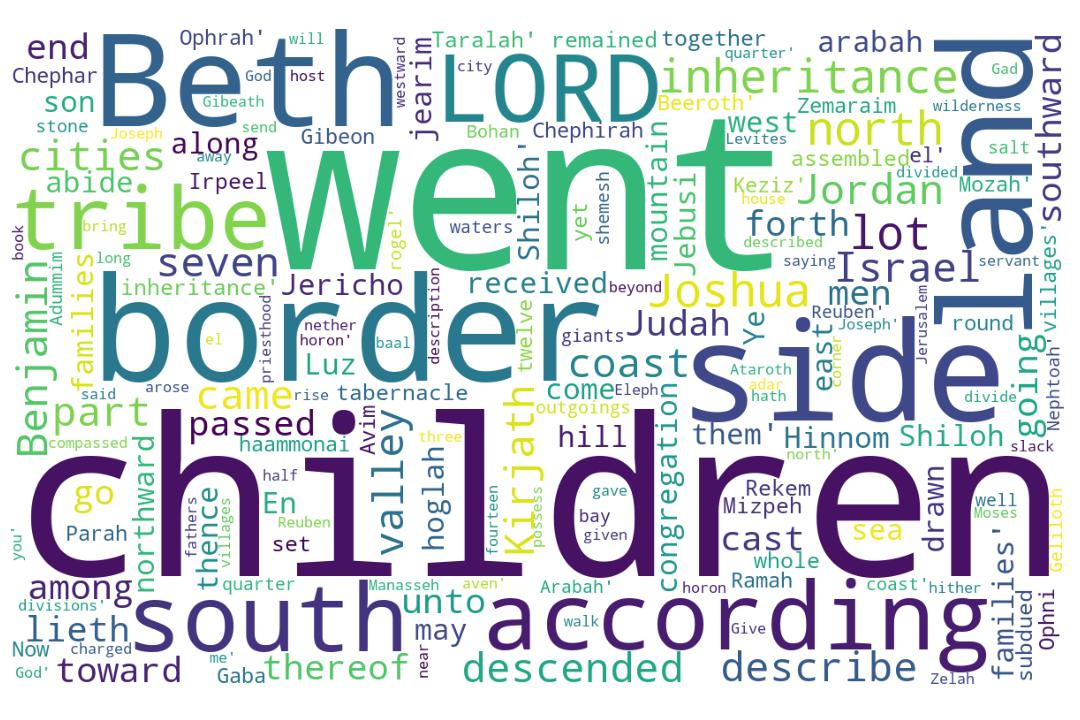
\includegraphics[width=\linewidth]{06OT-Joshua/Joshua18-WordCloud.jpg}
  \caption{Joshua 18 Word Cloud}
  \label{fig:Joshua 18 Word Cloud}
\end{figure}


\marginpar{\scriptsize \centering \fcolorbox{bone}{lime}{\textbf{LAND FOR BENJAMIN}}\\ (Joshua 18:1-28) \begin{compactenum}[I.][8]
	\item A Land \textbf{Subdued}  \index[scripture]{Joshua!Jsh 18:01} (Jsh 18:1) 
	\item A \textbf{Slackness}  \index[scripture]{Joshua!Jsh 18:03} (Jsh 18:3) 
	\item The \textbf{Scouts}  \index[scripture]{Joshua!Jsh 18:04} (Jsh 18:4) 
	\item  \textbf{Seven} Portions \index[scripture]{Joshua!Jsh 18:05} (Jsh 18:5) 
	\item The \textbf{Specfics}  \index[scripture]{Joshua!Jsh 18:11--28} (Jsh 18:11--28) 
	\item A Solid \textbf{Strategy} for Decisions -- analysis, counsel, prayer % \index[scripture]{Joshua!Jsh 18:11--28} (Jsh 18:11--28) 
\end{compactenum}}


\footnote{\textcolor[cmyk]{0.99998,1,0,0}{\hyperlink{TOC}{Return to end of Table of Contents.}}}\footnote{\href{https://audiobible.com/bible/joshua_18.html}{\textcolor[cmyk]{0.99998,1,0,0}{Joshua 18 Audio}}}\textcolor[cmyk]{0.99998,1,0,0}{And the whole congregation of the children of Israel assembled together at Shiloh, and set up the tabernacle of the congregation there. And the land was \fcolorbox{bone}{lime}{subdued} before them.}
[2] \textcolor[cmyk]{0.99998,1,0,0}{And there remained among the children of Israel seven tribes, which had not yet received their inheritance.}
[3] \textcolor[cmyk]{0.99998,1,0,0}{And Joshua said unto the children of Israel, How long \emph{are} ye \fcolorbox{bone}{lime}{slack} to go to possess the land, which the LORD God of your fathers hath given you?}
[4] \textcolor[cmyk]{0.99998,1,0,0}{Give out from among you three men for \emph{each} tribe: and I will send them, and they shall rise, and go \fcolorbox{bone}{lime}{through the land}, and describe it according to the inheritance of them; and they shall come \emph{again} to me.}
[5] \textcolor[cmyk]{0.99998,1,0,0}{And they shall divide it into \fcolorbox{bone}{lime}{seven parts}: Judah shall abide in their coast on the south, and the house of Joseph shall abide in their coasts on the north.}
[6] \textcolor[cmyk]{0.99998,1,0,0}{Ye shall therefore describe the land \emph{into} seven parts, and bring \emph{the} \emph{description} hither to me, that I may cast lots for you here before the LORD our God.}
[7] \textcolor[cmyk]{0.99998,1,0,0}{But the Levites have no part among you; for the priesthood of the LORD \emph{is} their inheritance: and Gad, and Reuben, and half the tribe of Manasseh, have received their inheritance beyond Jordan on the east, which Moses the servant of the LORD gave them.}\\
\\
\P \textcolor[cmyk]{0.99998,1,0,0}{And the men arose, and went away: and Joshua charged them that went to describe the land, saying, Go and walk through the land, and describe it, and come again to me, that I may here cast lots for you before the LORD in Shiloh.}
[9] \textcolor[cmyk]{0.99998,1,0,0}{And the men went and passed through the land, and described it by cities into seven parts in a book, and came \emph{again} to Joshua to the host at Shiloh.}\\
\\
\P \textcolor[cmyk]{0.99998,1,0,0}{And Joshua cast lots for them in Shiloh before the LORD: and there Joshua divided the land unto the children of Israel according to their divisions.}\\
\\
\P \textcolor[cmyk]{0.99998,1,0,0}{And \fcolorbox{bone}{lime}{the lot} of the tribe of the children of Benjamin came up according to their families: and the coast of their lot came forth between the children of Judah and the children of Joseph.}
[12] \textcolor[cmyk]{0.99998,1,0,0}{And their border on the north side was from Jordan; and the border went up to the side of Jericho on the north side, and went up through the mountains westward; and the goings out thereof were at the wilderness of Beth-aven.}
[13] \textcolor[cmyk]{0.99998,1,0,0}{And the border went over from thence toward Luz, to the side of Luz, which \emph{is} Beth-el, southward; and the border descended to Ataroth-adar, near the hill that \emph{lieth} on the south side of the nether Beth-horon.}
[14] \textcolor[cmyk]{0.99998,1,0,0}{And the border was drawn \emph{thence}, and compassed the corner of the sea southward, from the hill that \emph{lieth} before Beth-horon southward; and the goings out thereof were at Kirjath-baal, which \emph{is} Kirjath-jearim, a city of the children of Judah: this \emph{was} the west quarter.}
[15] \textcolor[cmyk]{0.99998,1,0,0}{And the south quarter \emph{was} from the end of Kirjath-jearim, and the border went out on the west, and went out to the well of waters of Nephtoah:}
[16] \textcolor[cmyk]{0.99998,1,0,0}{And the border came down to the end of the mountain that \emph{lieth} before the valley of the son of Hinnom, \emph{and} which \emph{is} in the valley of the giants on the north, and descended to the valley of Hinnom, to the side of Jebusi on the south, and descended to En-rogel,}
[17] \textcolor[cmyk]{0.99998,1,0,0}{And was drawn from the north, and went forth to En-shemesh, and went forth toward Geliloth, which \emph{is} over against the going up of Adummim, and descended to the stone of Bohan the son of Reuben,}
[18] \textcolor[cmyk]{0.99998,1,0,0}{And passed along toward the side over against Arabah northward, and went down unto Arabah:}
[19] \textcolor[cmyk]{0.99998,1,0,0}{And the border passed along to the side of Beth-hoglah northward: and the outgoings of the border were at the north bay of the salt sea at the south end of Jordan: this \emph{was} the south coast.}
[20] \textcolor[cmyk]{0.99998,1,0,0}{And Jordan was the border of it on the east side. This \emph{was} the inheritance of the children of Benjamin, by the coasts thereof round about, according to their families.}
[21] \textcolor[cmyk]{0.99998,1,0,0}{Now the cities of the tribe of the children of Benjamin according to their families were Jericho, and Beth-hoglah, and the valley of Keziz,}
[22] \textcolor[cmyk]{0.99998,1,0,0}{And Beth-arabah, and Zemaraim, and Beth-el,}
[23] \textcolor[cmyk]{0.99998,1,0,0}{And Avim, and Parah, and Ophrah,}
[24] \textcolor[cmyk]{0.99998,1,0,0}{And Chephar-haammonai, and Ophni, and Gaba; twelve cities with their villages:}
[25] \textcolor[cmyk]{0.99998,1,0,0}{Gibeon, and Ramah, and Beeroth,}
[26] \textcolor[cmyk]{0.99998,1,0,0}{And Mizpeh, and Chephirah, and Mozah,}
[27] \textcolor[cmyk]{0.99998,1,0,0}{And Rekem, and Irpeel, and Taralah,}
[28] \textcolor[cmyk]{0.99998,1,0,0}{And Zelah, Eleph, and Jebusi, which \emph{is} Jerusalem, Gibeath, \emph{and} Kirjath; fourteen cities with their villages. This \emph{is} the inheritance of the children of Benjamin according to their families.}

\index[NWIV]{29!Joshua!Jos 18:1}\index[AWIP]{And!Joshua!Jos 18:1}\index[AWIP]{And!Joshua!Jos 18:1 (2)}\index[AWIP]{the!Joshua!Jos 18:1}\index[AWIP]{the!Joshua!Jos 18:1 (2)}\index[AWIP]{the!Joshua!Jos 18:1 (3)}\index[AWIP]{the!Joshua!Jos 18:1 (4)}\index[AWIP]{the!Joshua!Jos 18:1 (5)}\index[AWIP]{whole!Joshua!Jos 18:1}\index[AWIP]{congregation!Joshua!Jos 18:1}\index[AWIP]{congregation!Joshua!Jos 18:1 (2)}\index[AWIP]{of!Joshua!Jos 18:1}\index[AWIP]{of!Joshua!Jos 18:1 (2)}\index[AWIP]{of!Joshua!Jos 18:1 (3)}\index[AWIP]{children!Joshua!Jos 18:1}\index[AWIP]{Israel!Joshua!Jos 18:1}\index[AWIP]{assembled!Joshua!Jos 18:1}\index[AWIP]{together!Joshua!Jos 18:1}\index[AWIP]{at!Joshua!Jos 18:1}\index[AWIP]{Shiloh!Joshua!Jos 18:1}\index[AWIP]{and!Joshua!Jos 18:1}\index[AWIP]{set!Joshua!Jos 18:1}\index[AWIP]{up!Joshua!Jos 18:1}\index[AWIP]{tabernacle!Joshua!Jos 18:1}\index[AWIP]{there!Joshua!Jos 18:1}\index[AWIP]{land!Joshua!Jos 18:1}\index[AWIP]{was!Joshua!Jos 18:1}\index[AWIP]{subdued!Joshua!Jos 18:1}\index[AWIP]{before!Joshua!Jos 18:1}\index[AWIP]{them!Joshua!Jos 18:1}

\index[NWIV]{17!Joshua!Jos 18:2}\index[AWIP]{And!Joshua!Jos 18:2}\index[AWIP]{there!Joshua!Jos 18:2}\index[AWIP]{remained!Joshua!Jos 18:2}\index[AWIP]{among!Joshua!Jos 18:2}\index[AWIP]{the!Joshua!Jos 18:2}\index[AWIP]{children!Joshua!Jos 18:2}\index[AWIP]{of!Joshua!Jos 18:2}\index[AWIP]{Israel!Joshua!Jos 18:2}\index[AWIP]{seven!Joshua!Jos 18:2}\index[AWIP]{tribes!Joshua!Jos 18:2}\index[AWIP]{which!Joshua!Jos 18:2}\index[AWIP]{had!Joshua!Jos 18:2}\index[AWIP]{not!Joshua!Jos 18:2}\index[AWIP]{yet!Joshua!Jos 18:2}\index[AWIP]{received!Joshua!Jos 18:2}\index[AWIP]{their!Joshua!Jos 18:2}\index[AWIP]{inheritance!Joshua!Jos 18:2}

\index[NWIV]{29!Joshua!Jos 18:3}\index[AWIP]{And!Joshua!Jos 18:3}\index[AWIP]{Joshua!Joshua!Jos 18:3}\index[AWIP]{said!Joshua!Jos 18:3}\index[AWIP]{unto!Joshua!Jos 18:3}\index[AWIP]{the!Joshua!Jos 18:3}\index[AWIP]{the!Joshua!Jos 18:3 (2)}\index[AWIP]{the!Joshua!Jos 18:3 (3)}\index[AWIP]{children!Joshua!Jos 18:3}\index[AWIP]{of!Joshua!Jos 18:3}\index[AWIP]{of!Joshua!Jos 18:3 (2)}\index[AWIP]{Israel!Joshua!Jos 18:3}\index[AWIP]{How!Joshua!Jos 18:3}\index[AWIP]{long!Joshua!Jos 18:3}\index[AWIP]{\emph{are}!Joshua!Jos 18:3}\index[AWIP]{ye!Joshua!Jos 18:3}\index[AWIP]{slack!Joshua!Jos 18:3}\index[AWIP]{to!Joshua!Jos 18:3}\index[AWIP]{to!Joshua!Jos 18:3 (2)}\index[AWIP]{go!Joshua!Jos 18:3}\index[AWIP]{possess!Joshua!Jos 18:3}\index[AWIP]{land!Joshua!Jos 18:3}\index[AWIP]{which!Joshua!Jos 18:3}\index[AWIP]{LORD!Joshua!Jos 18:3}\index[AWIP]{God!Joshua!Jos 18:3}\index[AWIP]{your!Joshua!Jos 18:3}\index[AWIP]{fathers!Joshua!Jos 18:3}\index[AWIP]{hath!Joshua!Jos 18:3}\index[AWIP]{given!Joshua!Jos 18:3}\index[AWIP]{you?!Joshua!Jos 18:3}\index[AWIP]{\emph{are}!Joshua!Jos 18:3}

\index[NWIV]{40!Joshua!Jos 18:4}\index[AWIP]{Give!Joshua!Jos 18:4}\index[AWIP]{out!Joshua!Jos 18:4}\index[AWIP]{from!Joshua!Jos 18:4}\index[AWIP]{among!Joshua!Jos 18:4}\index[AWIP]{you!Joshua!Jos 18:4}\index[AWIP]{three!Joshua!Jos 18:4}\index[AWIP]{men!Joshua!Jos 18:4}\index[AWIP]{for!Joshua!Jos 18:4}\index[AWIP]{\emph{each}!Joshua!Jos 18:4}\index[AWIP]{tribe!Joshua!Jos 18:4}\index[AWIP]{and!Joshua!Jos 18:4}\index[AWIP]{and!Joshua!Jos 18:4 (2)}\index[AWIP]{and!Joshua!Jos 18:4 (3)}\index[AWIP]{and!Joshua!Jos 18:4 (4)}\index[AWIP]{and!Joshua!Jos 18:4 (5)}\index[AWIP]{I!Joshua!Jos 18:4}\index[AWIP]{will!Joshua!Jos 18:4}\index[AWIP]{send!Joshua!Jos 18:4}\index[AWIP]{them!Joshua!Jos 18:4}\index[AWIP]{them!Joshua!Jos 18:4 (2)}\index[AWIP]{they!Joshua!Jos 18:4}\index[AWIP]{they!Joshua!Jos 18:4 (2)}\index[AWIP]{shall!Joshua!Jos 18:4}\index[AWIP]{shall!Joshua!Jos 18:4 (2)}\index[AWIP]{rise!Joshua!Jos 18:4}\index[AWIP]{go!Joshua!Jos 18:4}\index[AWIP]{through!Joshua!Jos 18:4}\index[AWIP]{the!Joshua!Jos 18:4}\index[AWIP]{the!Joshua!Jos 18:4 (2)}\index[AWIP]{land!Joshua!Jos 18:4}\index[AWIP]{describe!Joshua!Jos 18:4}\index[AWIP]{it!Joshua!Jos 18:4}\index[AWIP]{according!Joshua!Jos 18:4}\index[AWIP]{to!Joshua!Jos 18:4}\index[AWIP]{to!Joshua!Jos 18:4 (2)}\index[AWIP]{inheritance!Joshua!Jos 18:4}\index[AWIP]{of!Joshua!Jos 18:4}\index[AWIP]{come!Joshua!Jos 18:4}\index[AWIP]{\emph{again}!Joshua!Jos 18:4}\index[AWIP]{me!Joshua!Jos 18:4}\index[AWIP]{\emph{each}!Joshua!Jos 18:4}\index[AWIP]{\emph{again}!Joshua!Jos 18:4}

\index[NWIV]{30!Joshua!Jos 18:5}\index[AWIP]{And!Joshua!Jos 18:5}\index[AWIP]{they!Joshua!Jos 18:5}\index[AWIP]{shall!Joshua!Jos 18:5}\index[AWIP]{shall!Joshua!Jos 18:5 (2)}\index[AWIP]{shall!Joshua!Jos 18:5 (3)}\index[AWIP]{divide!Joshua!Jos 18:5}\index[AWIP]{it!Joshua!Jos 18:5}\index[AWIP]{into!Joshua!Jos 18:5}\index[AWIP]{seven!Joshua!Jos 18:5}\index[AWIP]{parts!Joshua!Jos 18:5}\index[AWIP]{Judah!Joshua!Jos 18:5}\index[AWIP]{abide!Joshua!Jos 18:5}\index[AWIP]{abide!Joshua!Jos 18:5 (2)}\index[AWIP]{in!Joshua!Jos 18:5}\index[AWIP]{in!Joshua!Jos 18:5 (2)}\index[AWIP]{their!Joshua!Jos 18:5}\index[AWIP]{their!Joshua!Jos 18:5 (2)}\index[AWIP]{coast!Joshua!Jos 18:5}\index[AWIP]{on!Joshua!Jos 18:5}\index[AWIP]{on!Joshua!Jos 18:5 (2)}\index[AWIP]{the!Joshua!Jos 18:5}\index[AWIP]{the!Joshua!Jos 18:5 (2)}\index[AWIP]{the!Joshua!Jos 18:5 (3)}\index[AWIP]{south!Joshua!Jos 18:5}\index[AWIP]{and!Joshua!Jos 18:5}\index[AWIP]{house!Joshua!Jos 18:5}\index[AWIP]{of!Joshua!Jos 18:5}\index[AWIP]{Joseph!Joshua!Jos 18:5}\index[AWIP]{coasts!Joshua!Jos 18:5}\index[AWIP]{north!Joshua!Jos 18:5}

\index[NWIV]{29!Joshua!Jos 18:6}\index[AWIP]{Ye!Joshua!Jos 18:6}\index[AWIP]{shall!Joshua!Jos 18:6}\index[AWIP]{therefore!Joshua!Jos 18:6}\index[AWIP]{describe!Joshua!Jos 18:6}\index[AWIP]{the!Joshua!Jos 18:6}\index[AWIP]{the!Joshua!Jos 18:6 (2)}\index[AWIP]{land!Joshua!Jos 18:6}\index[AWIP]{\emph{into}!Joshua!Jos 18:6}\index[AWIP]{seven!Joshua!Jos 18:6}\index[AWIP]{parts!Joshua!Jos 18:6}\index[AWIP]{and!Joshua!Jos 18:6}\index[AWIP]{bring!Joshua!Jos 18:6}\index[AWIP]{\emph{the}!Joshua!Jos 18:6}\index[AWIP]{\emph{description}!Joshua!Jos 18:6}\index[AWIP]{hither!Joshua!Jos 18:6}\index[AWIP]{to!Joshua!Jos 18:6}\index[AWIP]{me!Joshua!Jos 18:6}\index[AWIP]{that!Joshua!Jos 18:6}\index[AWIP]{I!Joshua!Jos 18:6}\index[AWIP]{may!Joshua!Jos 18:6}\index[AWIP]{cast!Joshua!Jos 18:6}\index[AWIP]{lots!Joshua!Jos 18:6}\index[AWIP]{for!Joshua!Jos 18:6}\index[AWIP]{you!Joshua!Jos 18:6}\index[AWIP]{here!Joshua!Jos 18:6}\index[AWIP]{before!Joshua!Jos 18:6}\index[AWIP]{LORD!Joshua!Jos 18:6}\index[AWIP]{our!Joshua!Jos 18:6}\index[AWIP]{God!Joshua!Jos 18:6}\index[AWIP]{\emph{into}!Joshua!Jos 18:6}\index[AWIP]{\emph{the}!Joshua!Jos 18:6}\index[AWIP]{\emph{description}!Joshua!Jos 18:6}

\index[NWIV]{45!Joshua!Jos 18:7}\index[AWIP]{But!Joshua!Jos 18:7}\index[AWIP]{the!Joshua!Jos 18:7}\index[AWIP]{the!Joshua!Jos 18:7 (2)}\index[AWIP]{the!Joshua!Jos 18:7 (3)}\index[AWIP]{the!Joshua!Jos 18:7 (4)}\index[AWIP]{the!Joshua!Jos 18:7 (5)}\index[AWIP]{the!Joshua!Jos 18:7 (6)}\index[AWIP]{the!Joshua!Jos 18:7 (7)}\index[AWIP]{Levites!Joshua!Jos 18:7}\index[AWIP]{have!Joshua!Jos 18:7}\index[AWIP]{have!Joshua!Jos 18:7 (2)}\index[AWIP]{no!Joshua!Jos 18:7}\index[AWIP]{part!Joshua!Jos 18:7}\index[AWIP]{among!Joshua!Jos 18:7}\index[AWIP]{you!Joshua!Jos 18:7}\index[AWIP]{for!Joshua!Jos 18:7}\index[AWIP]{priesthood!Joshua!Jos 18:7}\index[AWIP]{of!Joshua!Jos 18:7}\index[AWIP]{of!Joshua!Jos 18:7 (2)}\index[AWIP]{of!Joshua!Jos 18:7 (3)}\index[AWIP]{LORD!Joshua!Jos 18:7}\index[AWIP]{LORD!Joshua!Jos 18:7 (2)}\index[AWIP]{\emph{is}!Joshua!Jos 18:7}\index[AWIP]{their!Joshua!Jos 18:7}\index[AWIP]{their!Joshua!Jos 18:7 (2)}\index[AWIP]{inheritance!Joshua!Jos 18:7}\index[AWIP]{inheritance!Joshua!Jos 18:7 (2)}\index[AWIP]{and!Joshua!Jos 18:7}\index[AWIP]{and!Joshua!Jos 18:7 (2)}\index[AWIP]{and!Joshua!Jos 18:7 (3)}\index[AWIP]{Gad!Joshua!Jos 18:7}\index[AWIP]{Reuben!Joshua!Jos 18:7}\index[AWIP]{half!Joshua!Jos 18:7}\index[AWIP]{tribe!Joshua!Jos 18:7}\index[AWIP]{Manasseh!Joshua!Jos 18:7}\index[AWIP]{received!Joshua!Jos 18:7}\index[AWIP]{beyond!Joshua!Jos 18:7}\index[AWIP]{Jordan!Joshua!Jos 18:7}\index[AWIP]{on!Joshua!Jos 18:7}\index[AWIP]{east!Joshua!Jos 18:7}\index[AWIP]{which!Joshua!Jos 18:7}\index[AWIP]{Moses!Joshua!Jos 18:7}\index[AWIP]{servant!Joshua!Jos 18:7}\index[AWIP]{gave!Joshua!Jos 18:7}\index[AWIP]{them!Joshua!Jos 18:7}\index[AWIP]{\emph{is}!Joshua!Jos 18:7}

\index[NWIV]{45!Joshua!Jos 18:8}\index[AWIP]{And!Joshua!Jos 18:8}\index[AWIP]{the!Joshua!Jos 18:8}\index[AWIP]{the!Joshua!Jos 18:8 (2)}\index[AWIP]{the!Joshua!Jos 18:8 (3)}\index[AWIP]{the!Joshua!Jos 18:8 (4)}\index[AWIP]{men!Joshua!Jos 18:8}\index[AWIP]{arose!Joshua!Jos 18:8}\index[AWIP]{and!Joshua!Jos 18:8}\index[AWIP]{and!Joshua!Jos 18:8 (2)}\index[AWIP]{and!Joshua!Jos 18:8 (3)}\index[AWIP]{and!Joshua!Jos 18:8 (4)}\index[AWIP]{and!Joshua!Jos 18:8 (5)}\index[AWIP]{went!Joshua!Jos 18:8}\index[AWIP]{went!Joshua!Jos 18:8 (2)}\index[AWIP]{away!Joshua!Jos 18:8}\index[AWIP]{Joshua!Joshua!Jos 18:8}\index[AWIP]{charged!Joshua!Jos 18:8}\index[AWIP]{them!Joshua!Jos 18:8}\index[AWIP]{that!Joshua!Jos 18:8}\index[AWIP]{that!Joshua!Jos 18:8 (2)}\index[AWIP]{to!Joshua!Jos 18:8}\index[AWIP]{to!Joshua!Jos 18:8 (2)}\index[AWIP]{describe!Joshua!Jos 18:8}\index[AWIP]{describe!Joshua!Jos 18:8 (2)}\index[AWIP]{land!Joshua!Jos 18:8}\index[AWIP]{land!Joshua!Jos 18:8 (2)}\index[AWIP]{saying!Joshua!Jos 18:8}\index[AWIP]{Go!Joshua!Jos 18:8}\index[AWIP]{walk!Joshua!Jos 18:8}\index[AWIP]{through!Joshua!Jos 18:8}\index[AWIP]{it!Joshua!Jos 18:8}\index[AWIP]{come!Joshua!Jos 18:8}\index[AWIP]{again!Joshua!Jos 18:8}\index[AWIP]{me!Joshua!Jos 18:8}\index[AWIP]{I!Joshua!Jos 18:8}\index[AWIP]{may!Joshua!Jos 18:8}\index[AWIP]{here!Joshua!Jos 18:8}\index[AWIP]{cast!Joshua!Jos 18:8}\index[AWIP]{lots!Joshua!Jos 18:8}\index[AWIP]{for!Joshua!Jos 18:8}\index[AWIP]{you!Joshua!Jos 18:8}\index[AWIP]{before!Joshua!Jos 18:8}\index[AWIP]{LORD!Joshua!Jos 18:8}\index[AWIP]{in!Joshua!Jos 18:8}\index[AWIP]{Shiloh!Joshua!Jos 18:8}

\index[NWIV]{30!Joshua!Jos 18:9}\index[AWIP]{And!Joshua!Jos 18:9}\index[AWIP]{the!Joshua!Jos 18:9}\index[AWIP]{the!Joshua!Jos 18:9 (2)}\index[AWIP]{the!Joshua!Jos 18:9 (3)}\index[AWIP]{men!Joshua!Jos 18:9}\index[AWIP]{went!Joshua!Jos 18:9}\index[AWIP]{and!Joshua!Jos 18:9}\index[AWIP]{and!Joshua!Jos 18:9 (2)}\index[AWIP]{and!Joshua!Jos 18:9 (3)}\index[AWIP]{passed!Joshua!Jos 18:9}\index[AWIP]{through!Joshua!Jos 18:9}\index[AWIP]{land!Joshua!Jos 18:9}\index[AWIP]{described!Joshua!Jos 18:9}\index[AWIP]{it!Joshua!Jos 18:9}\index[AWIP]{by!Joshua!Jos 18:9}\index[AWIP]{cities!Joshua!Jos 18:9}\index[AWIP]{into!Joshua!Jos 18:9}\index[AWIP]{seven!Joshua!Jos 18:9}\index[AWIP]{parts!Joshua!Jos 18:9}\index[AWIP]{in!Joshua!Jos 18:9}\index[AWIP]{a!Joshua!Jos 18:9}\index[AWIP]{book!Joshua!Jos 18:9}\index[AWIP]{came!Joshua!Jos 18:9}\index[AWIP]{\emph{again}!Joshua!Jos 18:9}\index[AWIP]{to!Joshua!Jos 18:9}\index[AWIP]{to!Joshua!Jos 18:9 (2)}\index[AWIP]{Joshua!Joshua!Jos 18:9}\index[AWIP]{host!Joshua!Jos 18:9}\index[AWIP]{at!Joshua!Jos 18:9}\index[AWIP]{Shiloh!Joshua!Jos 18:9}\index[AWIP]{\emph{again}!Joshua!Jos 18:9}

\index[NWIV]{26!Joshua!Jos 18:10}\index[AWIP]{And!Joshua!Jos 18:10}\index[AWIP]{Joshua!Joshua!Jos 18:10}\index[AWIP]{Joshua!Joshua!Jos 18:10 (2)}\index[AWIP]{cast!Joshua!Jos 18:10}\index[AWIP]{lots!Joshua!Jos 18:10}\index[AWIP]{for!Joshua!Jos 18:10}\index[AWIP]{them!Joshua!Jos 18:10}\index[AWIP]{in!Joshua!Jos 18:10}\index[AWIP]{Shiloh!Joshua!Jos 18:10}\index[AWIP]{before!Joshua!Jos 18:10}\index[AWIP]{the!Joshua!Jos 18:10}\index[AWIP]{the!Joshua!Jos 18:10 (2)}\index[AWIP]{the!Joshua!Jos 18:10 (3)}\index[AWIP]{LORD!Joshua!Jos 18:10}\index[AWIP]{and!Joshua!Jos 18:10}\index[AWIP]{there!Joshua!Jos 18:10}\index[AWIP]{divided!Joshua!Jos 18:10}\index[AWIP]{land!Joshua!Jos 18:10}\index[AWIP]{unto!Joshua!Jos 18:10}\index[AWIP]{children!Joshua!Jos 18:10}\index[AWIP]{of!Joshua!Jos 18:10}\index[AWIP]{Israel!Joshua!Jos 18:10}\index[AWIP]{according!Joshua!Jos 18:10}\index[AWIP]{to!Joshua!Jos 18:10}\index[AWIP]{their!Joshua!Jos 18:10}\index[AWIP]{divisions!Joshua!Jos 18:10}

\index[NWIV]{35!Joshua!Jos 18:11}\index[AWIP]{And!Joshua!Jos 18:11}\index[AWIP]{the!Joshua!Jos 18:11}\index[AWIP]{the!Joshua!Jos 18:11 (2)}\index[AWIP]{the!Joshua!Jos 18:11 (3)}\index[AWIP]{the!Joshua!Jos 18:11 (4)}\index[AWIP]{the!Joshua!Jos 18:11 (5)}\index[AWIP]{the!Joshua!Jos 18:11 (6)}\index[AWIP]{lot!Joshua!Jos 18:11}\index[AWIP]{lot!Joshua!Jos 18:11 (2)}\index[AWIP]{of!Joshua!Jos 18:11}\index[AWIP]{of!Joshua!Jos 18:11 (2)}\index[AWIP]{of!Joshua!Jos 18:11 (3)}\index[AWIP]{of!Joshua!Jos 18:11 (4)}\index[AWIP]{of!Joshua!Jos 18:11 (5)}\index[AWIP]{of!Joshua!Jos 18:11 (6)}\index[AWIP]{tribe!Joshua!Jos 18:11}\index[AWIP]{children!Joshua!Jos 18:11}\index[AWIP]{children!Joshua!Jos 18:11 (2)}\index[AWIP]{children!Joshua!Jos 18:11 (3)}\index[AWIP]{Benjamin!Joshua!Jos 18:11}\index[AWIP]{came!Joshua!Jos 18:11}\index[AWIP]{came!Joshua!Jos 18:11 (2)}\index[AWIP]{up!Joshua!Jos 18:11}\index[AWIP]{according!Joshua!Jos 18:11}\index[AWIP]{to!Joshua!Jos 18:11}\index[AWIP]{their!Joshua!Jos 18:11}\index[AWIP]{their!Joshua!Jos 18:11 (2)}\index[AWIP]{families!Joshua!Jos 18:11}\index[AWIP]{and!Joshua!Jos 18:11}\index[AWIP]{and!Joshua!Jos 18:11 (2)}\index[AWIP]{coast!Joshua!Jos 18:11}\index[AWIP]{forth!Joshua!Jos 18:11}\index[AWIP]{between!Joshua!Jos 18:11}\index[AWIP]{Judah!Joshua!Jos 18:11}\index[AWIP]{Joseph!Joshua!Jos 18:11}

\index[NWIV]{42!Joshua!Jos 18:12}\index[AWIP]{And!Joshua!Jos 18:12}\index[AWIP]{their!Joshua!Jos 18:12}\index[AWIP]{border!Joshua!Jos 18:12}\index[AWIP]{border!Joshua!Jos 18:12 (2)}\index[AWIP]{on!Joshua!Jos 18:12}\index[AWIP]{on!Joshua!Jos 18:12 (2)}\index[AWIP]{the!Joshua!Jos 18:12}\index[AWIP]{the!Joshua!Jos 18:12 (2)}\index[AWIP]{the!Joshua!Jos 18:12 (3)}\index[AWIP]{the!Joshua!Jos 18:12 (4)}\index[AWIP]{the!Joshua!Jos 18:12 (5)}\index[AWIP]{the!Joshua!Jos 18:12 (6)}\index[AWIP]{the!Joshua!Jos 18:12 (7)}\index[AWIP]{north!Joshua!Jos 18:12}\index[AWIP]{north!Joshua!Jos 18:12 (2)}\index[AWIP]{side!Joshua!Jos 18:12}\index[AWIP]{side!Joshua!Jos 18:12 (2)}\index[AWIP]{side!Joshua!Jos 18:12 (3)}\index[AWIP]{was!Joshua!Jos 18:12}\index[AWIP]{from!Joshua!Jos 18:12}\index[AWIP]{Jordan!Joshua!Jos 18:12}\index[AWIP]{and!Joshua!Jos 18:12}\index[AWIP]{and!Joshua!Jos 18:12 (2)}\index[AWIP]{and!Joshua!Jos 18:12 (3)}\index[AWIP]{went!Joshua!Jos 18:12}\index[AWIP]{went!Joshua!Jos 18:12 (2)}\index[AWIP]{up!Joshua!Jos 18:12}\index[AWIP]{up!Joshua!Jos 18:12 (2)}\index[AWIP]{to!Joshua!Jos 18:12}\index[AWIP]{of!Joshua!Jos 18:12}\index[AWIP]{of!Joshua!Jos 18:12 (2)}\index[AWIP]{Jericho!Joshua!Jos 18:12}\index[AWIP]{through!Joshua!Jos 18:12}\index[AWIP]{mountains!Joshua!Jos 18:12}\index[AWIP]{westward!Joshua!Jos 18:12}\index[AWIP]{goings!Joshua!Jos 18:12}\index[AWIP]{out!Joshua!Jos 18:12}\index[AWIP]{thereof!Joshua!Jos 18:12}\index[AWIP]{were!Joshua!Jos 18:12}\index[AWIP]{at!Joshua!Jos 18:12}\index[AWIP]{wilderness!Joshua!Jos 18:12}\index[AWIP]{Beth-aven!Joshua!Jos 18:12}

\index[NWIV]{37!Joshua!Jos 18:13}\index[AWIP]{And!Joshua!Jos 18:13}\index[AWIP]{the!Joshua!Jos 18:13}\index[AWIP]{the!Joshua!Jos 18:13 (2)}\index[AWIP]{the!Joshua!Jos 18:13 (3)}\index[AWIP]{the!Joshua!Jos 18:13 (4)}\index[AWIP]{the!Joshua!Jos 18:13 (5)}\index[AWIP]{the!Joshua!Jos 18:13 (6)}\index[AWIP]{border!Joshua!Jos 18:13}\index[AWIP]{border!Joshua!Jos 18:13 (2)}\index[AWIP]{went!Joshua!Jos 18:13}\index[AWIP]{over!Joshua!Jos 18:13}\index[AWIP]{from!Joshua!Jos 18:13}\index[AWIP]{thence!Joshua!Jos 18:13}\index[AWIP]{toward!Joshua!Jos 18:13}\index[AWIP]{Luz!Joshua!Jos 18:13}\index[AWIP]{Luz!Joshua!Jos 18:13 (2)}\index[AWIP]{to!Joshua!Jos 18:13}\index[AWIP]{to!Joshua!Jos 18:13 (2)}\index[AWIP]{side!Joshua!Jos 18:13}\index[AWIP]{side!Joshua!Jos 18:13 (2)}\index[AWIP]{of!Joshua!Jos 18:13}\index[AWIP]{of!Joshua!Jos 18:13 (2)}\index[AWIP]{which!Joshua!Jos 18:13}\index[AWIP]{\emph{is}!Joshua!Jos 18:13}\index[AWIP]{Beth-el!Joshua!Jos 18:13}\index[AWIP]{southward!Joshua!Jos 18:13}\index[AWIP]{and!Joshua!Jos 18:13}\index[AWIP]{descended!Joshua!Jos 18:13}\index[AWIP]{Ataroth-adar!Joshua!Jos 18:13}\index[AWIP]{near!Joshua!Jos 18:13}\index[AWIP]{hill!Joshua!Jos 18:13}\index[AWIP]{that!Joshua!Jos 18:13}\index[AWIP]{\emph{lieth}!Joshua!Jos 18:13}\index[AWIP]{on!Joshua!Jos 18:13}\index[AWIP]{south!Joshua!Jos 18:13}\index[AWIP]{nether!Joshua!Jos 18:13}\index[AWIP]{Beth-horon!Joshua!Jos 18:13}\index[AWIP]{\emph{is}!Joshua!Jos 18:13}\index[AWIP]{\emph{lieth}!Joshua!Jos 18:13}

\index[NWIV]{45!Joshua!Jos 18:14}\index[AWIP]{And!Joshua!Jos 18:14}\index[AWIP]{the!Joshua!Jos 18:14}\index[AWIP]{the!Joshua!Jos 18:14 (2)}\index[AWIP]{the!Joshua!Jos 18:14 (3)}\index[AWIP]{the!Joshua!Jos 18:14 (4)}\index[AWIP]{the!Joshua!Jos 18:14 (5)}\index[AWIP]{the!Joshua!Jos 18:14 (6)}\index[AWIP]{the!Joshua!Jos 18:14 (7)}\index[AWIP]{border!Joshua!Jos 18:14}\index[AWIP]{was!Joshua!Jos 18:14}\index[AWIP]{drawn!Joshua!Jos 18:14}\index[AWIP]{\emph{thence}!Joshua!Jos 18:14}\index[AWIP]{and!Joshua!Jos 18:14}\index[AWIP]{and!Joshua!Jos 18:14 (2)}\index[AWIP]{compassed!Joshua!Jos 18:14}\index[AWIP]{corner!Joshua!Jos 18:14}\index[AWIP]{of!Joshua!Jos 18:14}\index[AWIP]{of!Joshua!Jos 18:14 (2)}\index[AWIP]{of!Joshua!Jos 18:14 (3)}\index[AWIP]{sea!Joshua!Jos 18:14}\index[AWIP]{southward!Joshua!Jos 18:14}\index[AWIP]{southward!Joshua!Jos 18:14 (2)}\index[AWIP]{from!Joshua!Jos 18:14}\index[AWIP]{hill!Joshua!Jos 18:14}\index[AWIP]{that!Joshua!Jos 18:14}\index[AWIP]{\emph{lieth}!Joshua!Jos 18:14}\index[AWIP]{before!Joshua!Jos 18:14}\index[AWIP]{Beth-horon!Joshua!Jos 18:14}\index[AWIP]{goings!Joshua!Jos 18:14}\index[AWIP]{out!Joshua!Jos 18:14}\index[AWIP]{thereof!Joshua!Jos 18:14}\index[AWIP]{were!Joshua!Jos 18:14}\index[AWIP]{at!Joshua!Jos 18:14}\index[AWIP]{Kirjath-baal!Joshua!Jos 18:14}\index[AWIP]{which!Joshua!Jos 18:14}\index[AWIP]{\emph{is}!Joshua!Jos 18:14}\index[AWIP]{Kirjath-jearim!Joshua!Jos 18:14}\index[AWIP]{a!Joshua!Jos 18:14}\index[AWIP]{city!Joshua!Jos 18:14}\index[AWIP]{children!Joshua!Jos 18:14}\index[AWIP]{Judah!Joshua!Jos 18:14}\index[AWIP]{this!Joshua!Jos 18:14}\index[AWIP]{\emph{was}!Joshua!Jos 18:14}\index[AWIP]{west!Joshua!Jos 18:14}\index[AWIP]{quarter!Joshua!Jos 18:14}\index[AWIP]{\emph{thence}!Joshua!Jos 18:14}\index[AWIP]{\emph{lieth}!Joshua!Jos 18:14}\index[AWIP]{\emph{is}!Joshua!Jos 18:14}\index[AWIP]{\emph{was}!Joshua!Jos 18:14}

\index[NWIV]{28!Joshua!Jos 18:15}\index[AWIP]{And!Joshua!Jos 18:15}\index[AWIP]{the!Joshua!Jos 18:15}\index[AWIP]{the!Joshua!Jos 18:15 (2)}\index[AWIP]{the!Joshua!Jos 18:15 (3)}\index[AWIP]{the!Joshua!Jos 18:15 (4)}\index[AWIP]{the!Joshua!Jos 18:15 (5)}\index[AWIP]{south!Joshua!Jos 18:15}\index[AWIP]{quarter!Joshua!Jos 18:15}\index[AWIP]{\emph{was}!Joshua!Jos 18:15}\index[AWIP]{from!Joshua!Jos 18:15}\index[AWIP]{end!Joshua!Jos 18:15}\index[AWIP]{of!Joshua!Jos 18:15}\index[AWIP]{of!Joshua!Jos 18:15 (2)}\index[AWIP]{of!Joshua!Jos 18:15 (3)}\index[AWIP]{Kirjath-jearim!Joshua!Jos 18:15}\index[AWIP]{and!Joshua!Jos 18:15}\index[AWIP]{and!Joshua!Jos 18:15 (2)}\index[AWIP]{border!Joshua!Jos 18:15}\index[AWIP]{went!Joshua!Jos 18:15}\index[AWIP]{went!Joshua!Jos 18:15 (2)}\index[AWIP]{out!Joshua!Jos 18:15}\index[AWIP]{out!Joshua!Jos 18:15 (2)}\index[AWIP]{on!Joshua!Jos 18:15}\index[AWIP]{west!Joshua!Jos 18:15}\index[AWIP]{to!Joshua!Jos 18:15}\index[AWIP]{well!Joshua!Jos 18:15}\index[AWIP]{waters!Joshua!Jos 18:15}\index[AWIP]{Nephtoah!Joshua!Jos 18:15}\index[AWIP]{\emph{was}!Joshua!Jos 18:15}

\index[NWIV]{52!Joshua!Jos 18:16}\index[AWIP]{And!Joshua!Jos 18:16}\index[AWIP]{the!Joshua!Jos 18:16}\index[AWIP]{the!Joshua!Jos 18:16 (2)}\index[AWIP]{the!Joshua!Jos 18:16 (3)}\index[AWIP]{the!Joshua!Jos 18:16 (4)}\index[AWIP]{the!Joshua!Jos 18:16 (5)}\index[AWIP]{the!Joshua!Jos 18:16 (6)}\index[AWIP]{the!Joshua!Jos 18:16 (7)}\index[AWIP]{the!Joshua!Jos 18:16 (8)}\index[AWIP]{the!Joshua!Jos 18:16 (9)}\index[AWIP]{the!Joshua!Jos 18:16 (10)}\index[AWIP]{the!Joshua!Jos 18:16 (11)}\index[AWIP]{border!Joshua!Jos 18:16}\index[AWIP]{came!Joshua!Jos 18:16}\index[AWIP]{down!Joshua!Jos 18:16}\index[AWIP]{to!Joshua!Jos 18:16}\index[AWIP]{to!Joshua!Jos 18:16 (2)}\index[AWIP]{to!Joshua!Jos 18:16 (3)}\index[AWIP]{to!Joshua!Jos 18:16 (4)}\index[AWIP]{end!Joshua!Jos 18:16}\index[AWIP]{of!Joshua!Jos 18:16}\index[AWIP]{of!Joshua!Jos 18:16 (2)}\index[AWIP]{of!Joshua!Jos 18:16 (3)}\index[AWIP]{of!Joshua!Jos 18:16 (4)}\index[AWIP]{of!Joshua!Jos 18:16 (5)}\index[AWIP]{of!Joshua!Jos 18:16 (6)}\index[AWIP]{mountain!Joshua!Jos 18:16}\index[AWIP]{that!Joshua!Jos 18:16}\index[AWIP]{\emph{lieth}!Joshua!Jos 18:16}\index[AWIP]{before!Joshua!Jos 18:16}\index[AWIP]{valley!Joshua!Jos 18:16}\index[AWIP]{valley!Joshua!Jos 18:16 (2)}\index[AWIP]{valley!Joshua!Jos 18:16 (3)}\index[AWIP]{son!Joshua!Jos 18:16}\index[AWIP]{Hinnom!Joshua!Jos 18:16}\index[AWIP]{Hinnom!Joshua!Jos 18:16 (2)}\index[AWIP]{\emph{and}!Joshua!Jos 18:16}\index[AWIP]{which!Joshua!Jos 18:16}\index[AWIP]{\emph{is}!Joshua!Jos 18:16}\index[AWIP]{in!Joshua!Jos 18:16}\index[AWIP]{giants!Joshua!Jos 18:16}\index[AWIP]{on!Joshua!Jos 18:16}\index[AWIP]{on!Joshua!Jos 18:16 (2)}\index[AWIP]{north!Joshua!Jos 18:16}\index[AWIP]{and!Joshua!Jos 18:16}\index[AWIP]{and!Joshua!Jos 18:16 (2)}\index[AWIP]{descended!Joshua!Jos 18:16}\index[AWIP]{descended!Joshua!Jos 18:16 (2)}\index[AWIP]{side!Joshua!Jos 18:16}\index[AWIP]{Jebusi!Joshua!Jos 18:16}\index[AWIP]{south!Joshua!Jos 18:16}\index[AWIP]{En-rogel!Joshua!Jos 18:16}\index[AWIP]{\emph{lieth}!Joshua!Jos 18:16}\index[AWIP]{\emph{and}!Joshua!Jos 18:16}\index[AWIP]{\emph{is}!Joshua!Jos 18:16}

\index[NWIV]{36!Joshua!Jos 18:17}\index[AWIP]{And!Joshua!Jos 18:17}\index[AWIP]{was!Joshua!Jos 18:17}\index[AWIP]{drawn!Joshua!Jos 18:17}\index[AWIP]{from!Joshua!Jos 18:17}\index[AWIP]{the!Joshua!Jos 18:17}\index[AWIP]{the!Joshua!Jos 18:17 (2)}\index[AWIP]{the!Joshua!Jos 18:17 (3)}\index[AWIP]{the!Joshua!Jos 18:17 (4)}\index[AWIP]{north!Joshua!Jos 18:17}\index[AWIP]{and!Joshua!Jos 18:17}\index[AWIP]{and!Joshua!Jos 18:17 (2)}\index[AWIP]{and!Joshua!Jos 18:17 (3)}\index[AWIP]{went!Joshua!Jos 18:17}\index[AWIP]{went!Joshua!Jos 18:17 (2)}\index[AWIP]{forth!Joshua!Jos 18:17}\index[AWIP]{forth!Joshua!Jos 18:17 (2)}\index[AWIP]{to!Joshua!Jos 18:17}\index[AWIP]{to!Joshua!Jos 18:17 (2)}\index[AWIP]{En-shemesh!Joshua!Jos 18:17}\index[AWIP]{toward!Joshua!Jos 18:17}\index[AWIP]{Geliloth!Joshua!Jos 18:17}\index[AWIP]{which!Joshua!Jos 18:17}\index[AWIP]{\emph{is}!Joshua!Jos 18:17}\index[AWIP]{over!Joshua!Jos 18:17}\index[AWIP]{against!Joshua!Jos 18:17}\index[AWIP]{going!Joshua!Jos 18:17}\index[AWIP]{up!Joshua!Jos 18:17}\index[AWIP]{of!Joshua!Jos 18:17}\index[AWIP]{of!Joshua!Jos 18:17 (2)}\index[AWIP]{of!Joshua!Jos 18:17 (3)}\index[AWIP]{Adummim!Joshua!Jos 18:17}\index[AWIP]{descended!Joshua!Jos 18:17}\index[AWIP]{stone!Joshua!Jos 18:17}\index[AWIP]{Bohan!Joshua!Jos 18:17}\index[AWIP]{son!Joshua!Jos 18:17}\index[AWIP]{Reuben!Joshua!Jos 18:17}\index[AWIP]{\emph{is}!Joshua!Jos 18:17}

\index[NWIV]{15!Joshua!Jos 18:18}\index[AWIP]{And!Joshua!Jos 18:18}\index[AWIP]{passed!Joshua!Jos 18:18}\index[AWIP]{along!Joshua!Jos 18:18}\index[AWIP]{toward!Joshua!Jos 18:18}\index[AWIP]{the!Joshua!Jos 18:18}\index[AWIP]{side!Joshua!Jos 18:18}\index[AWIP]{over!Joshua!Jos 18:18}\index[AWIP]{against!Joshua!Jos 18:18}\index[AWIP]{Arabah!Joshua!Jos 18:18}\index[AWIP]{Arabah!Joshua!Jos 18:18 (2)}\index[AWIP]{northward!Joshua!Jos 18:18}\index[AWIP]{and!Joshua!Jos 18:18}\index[AWIP]{went!Joshua!Jos 18:18}\index[AWIP]{down!Joshua!Jos 18:18}\index[AWIP]{unto!Joshua!Jos 18:18}

\index[NWIV]{37!Joshua!Jos 18:19}\index[AWIP]{And!Joshua!Jos 18:19}\index[AWIP]{the!Joshua!Jos 18:19}\index[AWIP]{the!Joshua!Jos 18:19 (2)}\index[AWIP]{the!Joshua!Jos 18:19 (3)}\index[AWIP]{the!Joshua!Jos 18:19 (4)}\index[AWIP]{the!Joshua!Jos 18:19 (5)}\index[AWIP]{the!Joshua!Jos 18:19 (6)}\index[AWIP]{the!Joshua!Jos 18:19 (7)}\index[AWIP]{the!Joshua!Jos 18:19 (8)}\index[AWIP]{border!Joshua!Jos 18:19}\index[AWIP]{border!Joshua!Jos 18:19 (2)}\index[AWIP]{passed!Joshua!Jos 18:19}\index[AWIP]{along!Joshua!Jos 18:19}\index[AWIP]{to!Joshua!Jos 18:19}\index[AWIP]{side!Joshua!Jos 18:19}\index[AWIP]{of!Joshua!Jos 18:19}\index[AWIP]{of!Joshua!Jos 18:19 (2)}\index[AWIP]{of!Joshua!Jos 18:19 (3)}\index[AWIP]{of!Joshua!Jos 18:19 (4)}\index[AWIP]{Beth-hoglah!Joshua!Jos 18:19}\index[AWIP]{northward!Joshua!Jos 18:19}\index[AWIP]{and!Joshua!Jos 18:19}\index[AWIP]{outgoings!Joshua!Jos 18:19}\index[AWIP]{were!Joshua!Jos 18:19}\index[AWIP]{at!Joshua!Jos 18:19}\index[AWIP]{at!Joshua!Jos 18:19 (2)}\index[AWIP]{north!Joshua!Jos 18:19}\index[AWIP]{bay!Joshua!Jos 18:19}\index[AWIP]{salt!Joshua!Jos 18:19}\index[AWIP]{sea!Joshua!Jos 18:19}\index[AWIP]{south!Joshua!Jos 18:19}\index[AWIP]{south!Joshua!Jos 18:19 (2)}\index[AWIP]{end!Joshua!Jos 18:19}\index[AWIP]{Jordan!Joshua!Jos 18:19}\index[AWIP]{this!Joshua!Jos 18:19}\index[AWIP]{\emph{was}!Joshua!Jos 18:19}\index[AWIP]{coast!Joshua!Jos 18:19}\index[AWIP]{\emph{was}!Joshua!Jos 18:19}

\index[NWIV]{30!Joshua!Jos 18:20}\index[AWIP]{And!Joshua!Jos 18:20}\index[AWIP]{Jordan!Joshua!Jos 18:20}\index[AWIP]{was!Joshua!Jos 18:20}\index[AWIP]{the!Joshua!Jos 18:20}\index[AWIP]{the!Joshua!Jos 18:20 (2)}\index[AWIP]{the!Joshua!Jos 18:20 (3)}\index[AWIP]{the!Joshua!Jos 18:20 (4)}\index[AWIP]{the!Joshua!Jos 18:20 (5)}\index[AWIP]{border!Joshua!Jos 18:20}\index[AWIP]{of!Joshua!Jos 18:20}\index[AWIP]{of!Joshua!Jos 18:20 (2)}\index[AWIP]{of!Joshua!Jos 18:20 (3)}\index[AWIP]{it!Joshua!Jos 18:20}\index[AWIP]{on!Joshua!Jos 18:20}\index[AWIP]{east!Joshua!Jos 18:20}\index[AWIP]{side!Joshua!Jos 18:20}\index[AWIP]{This!Joshua!Jos 18:20}\index[AWIP]{\emph{was}!Joshua!Jos 18:20}\index[AWIP]{inheritance!Joshua!Jos 18:20}\index[AWIP]{children!Joshua!Jos 18:20}\index[AWIP]{Benjamin!Joshua!Jos 18:20}\index[AWIP]{by!Joshua!Jos 18:20}\index[AWIP]{coasts!Joshua!Jos 18:20}\index[AWIP]{thereof!Joshua!Jos 18:20}\index[AWIP]{round!Joshua!Jos 18:20}\index[AWIP]{about!Joshua!Jos 18:20}\index[AWIP]{according!Joshua!Jos 18:20}\index[AWIP]{to!Joshua!Jos 18:20}\index[AWIP]{their!Joshua!Jos 18:20}\index[AWIP]{families!Joshua!Jos 18:20}\index[AWIP]{\emph{was}!Joshua!Jos 18:20}

\index[NWIV]{24!Joshua!Jos 18:21}\index[AWIP]{Now!Joshua!Jos 18:21}\index[AWIP]{the!Joshua!Jos 18:21}\index[AWIP]{the!Joshua!Jos 18:21 (2)}\index[AWIP]{the!Joshua!Jos 18:21 (3)}\index[AWIP]{the!Joshua!Jos 18:21 (4)}\index[AWIP]{cities!Joshua!Jos 18:21}\index[AWIP]{of!Joshua!Jos 18:21}\index[AWIP]{of!Joshua!Jos 18:21 (2)}\index[AWIP]{of!Joshua!Jos 18:21 (3)}\index[AWIP]{of!Joshua!Jos 18:21 (4)}\index[AWIP]{tribe!Joshua!Jos 18:21}\index[AWIP]{children!Joshua!Jos 18:21}\index[AWIP]{Benjamin!Joshua!Jos 18:21}\index[AWIP]{according!Joshua!Jos 18:21}\index[AWIP]{to!Joshua!Jos 18:21}\index[AWIP]{their!Joshua!Jos 18:21}\index[AWIP]{families!Joshua!Jos 18:21}\index[AWIP]{were!Joshua!Jos 18:21}\index[AWIP]{Jericho!Joshua!Jos 18:21}\index[AWIP]{and!Joshua!Jos 18:21}\index[AWIP]{and!Joshua!Jos 18:21 (2)}\index[AWIP]{Beth-hoglah!Joshua!Jos 18:21}\index[AWIP]{valley!Joshua!Jos 18:21}\index[AWIP]{Keziz!Joshua!Jos 18:21}

\index[NWIV]{6!Joshua!Jos 18:22}\index[AWIP]{And!Joshua!Jos 18:22}\index[AWIP]{Beth-arabah!Joshua!Jos 18:22}\index[AWIP]{and!Joshua!Jos 18:22}\index[AWIP]{and!Joshua!Jos 18:22 (2)}\index[AWIP]{Zemaraim!Joshua!Jos 18:22}\index[AWIP]{Beth-el!Joshua!Jos 18:22}

\index[NWIV]{6!Joshua!Jos 18:23}\index[AWIP]{And!Joshua!Jos 18:23}\index[AWIP]{Avim!Joshua!Jos 18:23}\index[AWIP]{and!Joshua!Jos 18:23}\index[AWIP]{and!Joshua!Jos 18:23 (2)}\index[AWIP]{Parah!Joshua!Jos 18:23}\index[AWIP]{Ophrah!Joshua!Jos 18:23}

\index[NWIV]{11!Joshua!Jos 18:24}\index[AWIP]{And!Joshua!Jos 18:24}\index[AWIP]{Chephar-haammonai!Joshua!Jos 18:24}\index[AWIP]{and!Joshua!Jos 18:24}\index[AWIP]{and!Joshua!Jos 18:24 (2)}\index[AWIP]{Ophni!Joshua!Jos 18:24}\index[AWIP]{Gaba!Joshua!Jos 18:24}\index[AWIP]{twelve!Joshua!Jos 18:24}\index[AWIP]{cities!Joshua!Jos 18:24}\index[AWIP]{with!Joshua!Jos 18:24}\index[AWIP]{their!Joshua!Jos 18:24}\index[AWIP]{villages!Joshua!Jos 18:24}

\index[NWIV]{5!Joshua!Jos 18:25}\index[AWIP]{Gibeon!Joshua!Jos 18:25}\index[AWIP]{and!Joshua!Jos 18:25}\index[AWIP]{and!Joshua!Jos 18:25 (2)}\index[AWIP]{Ramah!Joshua!Jos 18:25}\index[AWIP]{Beeroth!Joshua!Jos 18:25}

\index[NWIV]{6!Joshua!Jos 18:26}\index[AWIP]{And!Joshua!Jos 18:26}\index[AWIP]{Mizpeh!Joshua!Jos 18:26}\index[AWIP]{and!Joshua!Jos 18:26}\index[AWIP]{and!Joshua!Jos 18:26 (2)}\index[AWIP]{Chephirah!Joshua!Jos 18:26}\index[AWIP]{Mozah!Joshua!Jos 18:26}

\index[NWIV]{6!Joshua!Jos 18:27}\index[AWIP]{And!Joshua!Jos 18:27}\index[AWIP]{Rekem!Joshua!Jos 18:27}\index[AWIP]{and!Joshua!Jos 18:27}\index[AWIP]{and!Joshua!Jos 18:27 (2)}\index[AWIP]{Irpeel!Joshua!Jos 18:27}\index[AWIP]{Taralah!Joshua!Jos 18:27}

\index[NWIV]{29!Joshua!Jos 18:28}\index[AWIP]{And!Joshua!Jos 18:28}\index[AWIP]{Zelah!Joshua!Jos 18:28}\index[AWIP]{Eleph!Joshua!Jos 18:28}\index[AWIP]{and!Joshua!Jos 18:28}\index[AWIP]{Jebusi!Joshua!Jos 18:28}\index[AWIP]{which!Joshua!Jos 18:28}\index[AWIP]{\emph{is}!Joshua!Jos 18:28}\index[AWIP]{\emph{is}!Joshua!Jos 18:28 (2)}\index[AWIP]{Jerusalem!Joshua!Jos 18:28}\index[AWIP]{Gibeath!Joshua!Jos 18:28}\index[AWIP]{\emph{and}!Joshua!Jos 18:28}\index[AWIP]{Kirjath!Joshua!Jos 18:28}\index[AWIP]{fourteen!Joshua!Jos 18:28}\index[AWIP]{cities!Joshua!Jos 18:28}\index[AWIP]{with!Joshua!Jos 18:28}\index[AWIP]{their!Joshua!Jos 18:28}\index[AWIP]{their!Joshua!Jos 18:28 (2)}\index[AWIP]{villages!Joshua!Jos 18:28}\index[AWIP]{This!Joshua!Jos 18:28}\index[AWIP]{the!Joshua!Jos 18:28}\index[AWIP]{the!Joshua!Jos 18:28 (2)}\index[AWIP]{inheritance!Joshua!Jos 18:28}\index[AWIP]{of!Joshua!Jos 18:28}\index[AWIP]{of!Joshua!Jos 18:28 (2)}\index[AWIP]{children!Joshua!Jos 18:28}\index[AWIP]{Benjamin!Joshua!Jos 18:28}\index[AWIP]{according!Joshua!Jos 18:28}\index[AWIP]{to!Joshua!Jos 18:28}\index[AWIP]{families!Joshua!Jos 18:28}\index[AWIP]{\emph{is}!Joshua!Jos 18:28}\index[AWIP]{\emph{is}!Joshua!Jos 18:28 (2)}\index[AWIP]{\emph{and}!Joshua!Jos 18:28}


\section{Joshua 18 Outlines}

\subsection{My Outlines}

\subsubsection{Land for Benjamin}
\index[speaker]{Keith Anthony!Joshua 18 (Land for Benjamin}
\index[series]{Joshua (Keith Anthony)!Joshua 18 (Land for Benjamin)}
\index[date]{2018/03/12!Joshua 18 (Land for Benjamin) (Keith Anthony)}
\begin{compactenum}[I.]
	\item A Land \textbf{Subdued}  \index[scripture]{Joshua!Jsh 18:01} (Jsh 18:1) 
	\item A \textbf{Slackness}  \index[scripture]{Joshua!Jsh 18:03} (Jsh 18:3) 
	\item The \textbf{Scouts}  \index[scripture]{Joshua!Jsh 18:04} (Jsh 18:4) 
	\item  \textbf{Seven} Portions \index[scripture]{Joshua!Jsh 18:05} (Jsh 18:5) 
	\item The \textbf{Specfics}  \index[scripture]{Joshua!Jsh 18:11--28} (Jsh 18:11--28) 
	\item A Solid \textbf{Strategy} for Decisions -- analysis, counsel, prayer % \index[scripture]{Joshua!Jsh 18:11--28} (Jsh 18:11--28) 
\end{compactenum}
\subsection{My Outlines from Others}


\section{Joshua 18 Comments}


\subsection{Joshua 18 Repeated Phrases}


%%%%%%%%%%
%%%%%%%%%%
\normalsize
 
\begin{center}
\begin{longtable}{|p{3.0in}|p{0.5in}|}
\caption[Joshua 18 Repeated Phrases]{Joshua 18 Repeated Phrases}\label{table:Repeated Phrases Joshua 18} \\
\hline \multicolumn{1}{|c|}{\textbf{Phrase}} & \multicolumn{1}{c|}{\textbf{Frequency}} \\ \hline 
\endfirsthead
 
\multicolumn{2}{c}
{{\bfseries \tablename\ \thetable{} -- continued from previous page}} \\  
\hline \multicolumn{1}{|c|}{\textbf{Phrase}} & \multicolumn{1}{c|}{\textbf{Frequency}} \\ \hline 
\endhead
 
\hline \multicolumn{2}{c}{{ }} \\ \hline
\endfoot 
of the & 18\\ \hline 
the children & 11\\ \hline 
the children of & 11\\ \hline 
children of & 11\\ \hline 
And the & 10\\ \hline 
to the & 10\\ \hline 
on the & 10\\ \hline 
and the & 10\\ \hline 
the border & 9\\ \hline 
the land & 8\\ \hline 
of the children & 6\\ \hline 
of the children of & 6\\ \hline 
the LORD & 6\\ \hline 
according to & 6\\ \hline 
the south & 6\\ \hline 
the north & 6\\ \hline 
and went & 6\\ \hline 
according to their & 5\\ \hline 
to their & 5\\ \hline 
the side & 5\\ \hline 
side of & 5\\ \hline 
which \emph{is} & 5\\ \hline 
the children of Israel & 4\\ \hline 
children of Israel & 4\\ \hline 
of Israel & 4\\ \hline 
through the & 4\\ \hline 
on the north & 4\\ \hline 
before the & 4\\ \hline 
of the children of Benjamin & 4\\ \hline 
the children of Benjamin & 4\\ \hline 
children of Benjamin & 4\\ \hline 
of Benjamin & 4\\ \hline 
according to their families & 4\\ \hline 
to their families & 4\\ \hline 
their families & 4\\ \hline 
to the side & 4\\ \hline 
to the side of & 4\\ \hline 
the side of & 4\\ \hline 
And the border & 4\\ \hline 
descended to & 4\\ \hline 
the valley & 4\\ \hline 
the valley of & 4\\ \hline 
valley of & 4\\ \hline 
their inheritance & 3\\ \hline 
they shall & 3\\ \hline 
through the land & 3\\ \hline 
through the land and & 3\\ \hline 
the land and & 3\\ \hline 
land and & 3\\ \hline 
the inheritance & 3\\ \hline 
the inheritance of & 3\\ \hline 
inheritance of & 3\\ \hline 
to me & 3\\ \hline 
seven parts & 3\\ \hline 
on the south & 3\\ \hline 
cast lots & 3\\ \hline 
cast lots for & 3\\ \hline 
lots for & 3\\ \hline 
before the LORD & 3\\ \hline 
the tribe & 3\\ \hline 
the tribe of & 3\\ \hline 
tribe of & 3\\ \hline 
and the border & 3\\ \hline 
the border went & 3\\ \hline 
border went & 3\\ \hline 
were at & 3\\ \hline 
at the & 3\\ \hline 
that \emph{lieth} & 3\\ \hline 
from the & 3\\ \hline 
\emph{was} the & 3\\ \hline 
end of & 3\\ \hline 
and descended & 3\\ \hline 
and descended to & 3\\ \hline 
\end{longtable}
\end{center}



%%%%%%%%%%
%%%%%%%%%%



\section{Joshua 18 Word Statistics}


%%%%%%%%%%
%%%%%%%%%%
\normalsize
 
\begin{center}
\begin{longtable}{l|c|c|c|c}
\caption[Joshua 18 Statistics]{Joshua 18 Statistics}\label{table:Statistics for Joshua 18} \\
\hline \multicolumn{1}{|c|}{\textbf{Verse(s)}} & \multicolumn{1}{|c|}{\textbf{Count}} & \multicolumn{1}{|c|}{\textbf{Unique}} & \multicolumn{1}{|c|}{\textbf{Italics}} & \multicolumn{1}{|c|}{\textbf{Uniq Italic}}  \\ \hline 
\endfirsthead
 
\multicolumn{5}{c}
{{\bfseries \tablename\ \thetable{} -- continued from previous page}} \\  
\hline \multicolumn{1}{|c|}{\textbf{Verse(s)}} & \multicolumn{1}{|c|}{\textbf{Count}} & \multicolumn{1}{|c|}{\textbf{Unique}} & \multicolumn{1}{|c|}{\textbf{Italics}} & \multicolumn{1}{|c|}{\textbf{Uniq Italic}}  \\ \hline 
\endhead
 
\hline \multicolumn{5}{|r|}{{Continued if needed}} \\ \hline
\endfoot 
1 & 29 & 21 & 0 & 0\\ \hline
2 & 17 & 17 & 0 & 0\\ \hline
3 & 29 & 25 & 1 & 1\\ \hline
4 & 40 & 31 & 2 & 2\\ \hline
5 & 30 & 22 & 0 & 0\\ \hline
6 & 29 & 28 & 3 & 3\\ \hline
7 & 45 & 31 & 1 & 1\\ \hline
8 & 45 & 33 & 0 & 0\\ \hline
9 & 30 & 25 & 1 & 1\\ \hline
10 & 26 & 23 & 0 & 0\\ \hline
11 & 35 & 19 & 0 & 0\\ \hline
12 & 42 & 26 & 0 & 0\\ \hline
13 & 37 & 27 & 2 & 2\\ \hline
14 & 45 & 35 & 4 & 4\\ \hline
15 & 28 & 19 & 1 & 1\\ \hline
16 & 52 & 28 & 3 & 3\\ \hline
17 & 36 & 26 & 1 & 1\\ \hline
18 & 15 & 14 & 0 & 0\\ \hline
19 & 37 & 24 & 1 & 1\\ \hline
20 & 30 & 24 & 1 & 1\\ \hline
21 & 24 & 17 & 0 & 0\\ \hline
22 & 6 & 5 & 0 & 0\\ \hline
23 & 6 & 5 & 0 & 0\\ \hline
24 & 11 & 10 & 0 & 0\\ \hline
25 & 5 & 4 & 0 & 0\\ \hline
26 & 6 & 5 & 0 & 0\\ \hline
27 & 6 & 5 & 0 & 0\\ \hline
28 & 29 & 25 & 3 & 2\\ \hline
Total & 770 & 230 & 24 & 11
\end{longtable}
\end{center}



%%%%%%%%%%
%%%%%%%%%%


\subsection{Joshua 18 Words by Frequency}


%%%%%%%%%%
%%%%%%%%%%
\normalsize
 
\begin{center}
\begin{longtable}{l|r}
\caption[Joshua 18 Words by Frequency]{Joshua 18 Words by Frequency}\label{table:WordsbyFrequency for Joshua 18} \\
\hline \multicolumn{1}{|c|}{\textbf{Word}} & \multicolumn{1}{c|}{\textbf{Frequency}} \\ \hline 
\endfirsthead
 
\multicolumn{2}{c}
{{\bfseries \tablename\ \thetable{} -- continued from previous page}} \\  
\hline \multicolumn{1}{|c|}{\textbf{Word}} & \multicolumn{1}{c|}{\textbf{Frequency}} \\ \hline 
\endhead
 
\hline \multicolumn{2}{c}{{ }} \\ \hline
\endfoot 
the & 99\\ \hline 
and & 52\\ \hline 
of & 50\\ \hline 
to & 25\\ \hline 
And & 24\\ \hline 
their & 14\\ \hline 
children & 11\\ \hline 
went & 11\\ \hline 
on & 10\\ \hline 
border & 10\\ \hline 
side & 9\\ \hline 
land & 8\\ \hline 
which & 8\\ \hline 
\emph{is} & 7\\ \hline 
at & 6\\ \hline 
before & 6\\ \hline 
them & 6\\ \hline 
inheritance & 6\\ \hline 
LORD & 6\\ \hline 
from & 6\\ \hline 
shall & 6\\ \hline 
according & 6\\ \hline 
in & 6\\ \hline 
south & 6\\ \hline 
north & 6\\ \hline 
that & 6\\ \hline 
up & 5\\ \hline 
was & 5\\ \hline 
Joshua & 5\\ \hline 
you & 5\\ \hline 
out & 5\\ \hline 
for & 5\\ \hline 
it & 5\\ \hline 
Israel & 4\\ \hline 
Shiloh & 4\\ \hline 
seven & 4\\ \hline 
tribe & 4\\ \hline 
through & 4\\ \hline 
describe & 4\\ \hline 
Jordan & 4\\ \hline 
cities & 4\\ \hline 
came & 4\\ \hline 
Benjamin & 4\\ \hline 
families & 4\\ \hline 
were & 4\\ \hline 
descended & 4\\ \hline 
\emph{was} & 4\\ \hline 
valley & 4\\ \hline 
there & 3\\ \hline 
among & 3\\ \hline 
unto & 3\\ \hline 
men & 3\\ \hline 
I & 3\\ \hline 
they & 3\\ \hline 
me & 3\\ \hline 
parts & 3\\ \hline 
Judah & 3\\ \hline 
coast & 3\\ \hline 
cast & 3\\ \hline 
lots & 3\\ \hline 
passed & 3\\ \hline 
forth & 3\\ \hline 
thereof & 3\\ \hline 
over & 3\\ \hline 
toward & 3\\ \hline 
southward & 3\\ \hline 
\emph{lieth} & 3\\ \hline 
end & 3\\ \hline 
congregation & 2\\ \hline 
received & 2\\ \hline 
go & 2\\ \hline 
God & 2\\ \hline 
come & 2\\ \hline 
\emph{again} & 2\\ \hline 
into & 2\\ \hline 
abide & 2\\ \hline 
Joseph & 2\\ \hline 
coasts & 2\\ \hline 
may & 2\\ \hline 
here & 2\\ \hline 
have & 2\\ \hline 
Reuben & 2\\ \hline 
east & 2\\ \hline 
by & 2\\ \hline 
a & 2\\ \hline 
lot & 2\\ \hline 
Jericho & 2\\ \hline 
goings & 2\\ \hline 
Luz & 2\\ \hline 
Beth-el & 2\\ \hline 
hill & 2\\ \hline 
Beth-horon & 2\\ \hline 
drawn & 2\\ \hline 
sea & 2\\ \hline 
Kirjath-jearim & 2\\ \hline 
this & 2\\ \hline 
west & 2\\ \hline 
quarter & 2\\ \hline 
down & 2\\ \hline 
son & 2\\ \hline 
Hinnom & 2\\ \hline 
\emph{and} & 2\\ \hline 
Jebusi & 2\\ \hline 
against & 2\\ \hline 
along & 2\\ \hline 
Arabah & 2\\ \hline 
northward & 2\\ \hline 
Beth-hoglah & 2\\ \hline 
This & 2\\ \hline 
with & 2\\ \hline 
villages & 2\\ \hline 
whole & 1\\ \hline 
assembled & 1\\ \hline 
together & 1\\ \hline 
set & 1\\ \hline 
tabernacle & 1\\ \hline 
subdued & 1\\ \hline 
remained & 1\\ \hline 
tribes & 1\\ \hline 
had & 1\\ \hline 
not & 1\\ \hline 
yet & 1\\ \hline 
said & 1\\ \hline 
How & 1\\ \hline 
long & 1\\ \hline 
\emph{are} & 1\\ \hline 
ye & 1\\ \hline 
slack & 1\\ \hline 
possess & 1\\ \hline 
your & 1\\ \hline 
fathers & 1\\ \hline 
hath & 1\\ \hline 
given & 1\\ \hline 
Give & 1\\ \hline 
three & 1\\ \hline 
\emph{each} & 1\\ \hline 
will & 1\\ \hline 
send & 1\\ \hline 
rise & 1\\ \hline 
divide & 1\\ \hline 
house & 1\\ \hline 
Ye & 1\\ \hline 
therefore & 1\\ \hline 
\emph{into} & 1\\ \hline 
bring & 1\\ \hline 
\emph{the} & 1\\ \hline 
\emph{description} & 1\\ \hline 
hither & 1\\ \hline 
our & 1\\ \hline 
But & 1\\ \hline 
Levites & 1\\ \hline 
no & 1\\ \hline 
part & 1\\ \hline 
priesthood & 1\\ \hline 
Gad & 1\\ \hline 
half & 1\\ \hline 
Manasseh & 1\\ \hline 
beyond & 1\\ \hline 
Moses & 1\\ \hline 
servant & 1\\ \hline 
gave & 1\\ \hline 
arose & 1\\ \hline 
away & 1\\ \hline 
charged & 1\\ \hline 
saying & 1\\ \hline 
Go & 1\\ \hline 
walk & 1\\ \hline 
again & 1\\ \hline 
described & 1\\ \hline 
book & 1\\ \hline 
host & 1\\ \hline 
divided & 1\\ \hline 
divisions & 1\\ \hline 
between & 1\\ \hline 
mountains & 1\\ \hline 
westward & 1\\ \hline 
wilderness & 1\\ \hline 
Beth-aven & 1\\ \hline 
thence & 1\\ \hline 
Ataroth-adar & 1\\ \hline 
near & 1\\ \hline 
nether & 1\\ \hline 
\emph{thence} & 1\\ \hline 
compassed & 1\\ \hline 
corner & 1\\ \hline 
Kirjath-baal & 1\\ \hline 
city & 1\\ \hline 
well & 1\\ \hline 
waters & 1\\ \hline 
Nephtoah & 1\\ \hline 
mountain & 1\\ \hline 
giants & 1\\ \hline 
En-rogel & 1\\ \hline 
En-shemesh & 1\\ \hline 
Geliloth & 1\\ \hline 
going & 1\\ \hline 
Adummim & 1\\ \hline 
stone & 1\\ \hline 
Bohan & 1\\ \hline 
outgoings & 1\\ \hline 
bay & 1\\ \hline 
salt & 1\\ \hline 
round & 1\\ \hline 
about & 1\\ \hline 
Now & 1\\ \hline 
Keziz & 1\\ \hline 
Beth-arabah & 1\\ \hline 
Zemaraim & 1\\ \hline 
Avim & 1\\ \hline 
Parah & 1\\ \hline 
Ophrah & 1\\ \hline 
Chephar-haammonai & 1\\ \hline 
Ophni & 1\\ \hline 
Gaba & 1\\ \hline 
twelve & 1\\ \hline 
Gibeon & 1\\ \hline 
Ramah & 1\\ \hline 
Beeroth & 1\\ \hline 
Mizpeh & 1\\ \hline 
Chephirah & 1\\ \hline 
Mozah & 1\\ \hline 
Rekem & 1\\ \hline 
Irpeel & 1\\ \hline 
Taralah & 1\\ \hline 
Zelah & 1\\ \hline 
Eleph & 1\\ \hline 
Jerusalem & 1\\ \hline 
Gibeath & 1\\ \hline 
Kirjath & 1\\ \hline 
fourteen & 1\\ \hline 
\end{longtable}
\end{center}



%%%%%%%%%%
%%%%%%%%%%


\subsection{Joshua 18 Words Alphabetically}


%%%%%%%%%%
%%%%%%%%%%
\normalsize
 
\begin{center}
\begin{longtable}{l|r}
\caption[Joshua 18 Words Alphabetically]{Joshua 18 Words Alphabetically}\label{table:WordsAlphabetically for Joshua 18} \\
\hline \multicolumn{1}{|c|}{\textbf{Word}} & \multicolumn{1}{c|}{\textbf{Frequency}} \\ \hline 
\endfirsthead
 
\multicolumn{2}{c}
{{\bfseries \tablename\ \thetable{} -- continued from previous page}} \\  
\hline \multicolumn{1}{|c|}{\textbf{Word}} & \multicolumn{1}{c|}{\textbf{Frequency}} \\ \hline 
\endhead
 
\hline \multicolumn{2}{c}{{ }} \\ \hline
\endfoot 
Adummim & 1\\ \hline 
And & 24\\ \hline 
Arabah & 2\\ \hline 
Ataroth-adar & 1\\ \hline 
Avim & 1\\ \hline 
Beeroth & 1\\ \hline 
Benjamin & 4\\ \hline 
Beth-arabah & 1\\ \hline 
Beth-aven & 1\\ \hline 
Beth-el & 2\\ \hline 
Beth-hoglah & 2\\ \hline 
Beth-horon & 2\\ \hline 
Bohan & 1\\ \hline 
But & 1\\ \hline 
Chephar-haammonai & 1\\ \hline 
Chephirah & 1\\ \hline 
Eleph & 1\\ \hline 
En-rogel & 1\\ \hline 
En-shemesh & 1\\ \hline 
Gaba & 1\\ \hline 
Gad & 1\\ \hline 
Geliloth & 1\\ \hline 
Gibeath & 1\\ \hline 
Gibeon & 1\\ \hline 
Give & 1\\ \hline 
Go & 1\\ \hline 
God & 2\\ \hline 
Hinnom & 2\\ \hline 
How & 1\\ \hline 
I & 3\\ \hline 
Irpeel & 1\\ \hline 
Israel & 4\\ \hline 
Jebusi & 2\\ \hline 
Jericho & 2\\ \hline 
Jerusalem & 1\\ \hline 
Jordan & 4\\ \hline 
Joseph & 2\\ \hline 
Joshua & 5\\ \hline 
Judah & 3\\ \hline 
Keziz & 1\\ \hline 
Kirjath & 1\\ \hline 
Kirjath-baal & 1\\ \hline 
Kirjath-jearim & 2\\ \hline 
LORD & 6\\ \hline 
Levites & 1\\ \hline 
Luz & 2\\ \hline 
Manasseh & 1\\ \hline 
Mizpeh & 1\\ \hline 
Moses & 1\\ \hline 
Mozah & 1\\ \hline 
Nephtoah & 1\\ \hline 
Now & 1\\ \hline 
Ophni & 1\\ \hline 
Ophrah & 1\\ \hline 
Parah & 1\\ \hline 
Ramah & 1\\ \hline 
Rekem & 1\\ \hline 
Reuben & 2\\ \hline 
Shiloh & 4\\ \hline 
Taralah & 1\\ \hline 
This & 2\\ \hline 
Ye & 1\\ \hline 
Zelah & 1\\ \hline 
Zemaraim & 1\\ \hline 
\emph{again} & 2\\ \hline 
\emph{and} & 2\\ \hline 
\emph{are} & 1\\ \hline 
\emph{description} & 1\\ \hline 
\emph{each} & 1\\ \hline 
\emph{into} & 1\\ \hline 
\emph{is} & 7\\ \hline 
\emph{lieth} & 3\\ \hline 
\emph{thence} & 1\\ \hline 
\emph{the} & 1\\ \hline 
\emph{was} & 4\\ \hline 
a & 2\\ \hline 
abide & 2\\ \hline 
about & 1\\ \hline 
according & 6\\ \hline 
again & 1\\ \hline 
against & 2\\ \hline 
along & 2\\ \hline 
among & 3\\ \hline 
and & 52\\ \hline 
arose & 1\\ \hline 
assembled & 1\\ \hline 
at & 6\\ \hline 
away & 1\\ \hline 
bay & 1\\ \hline 
before & 6\\ \hline 
between & 1\\ \hline 
beyond & 1\\ \hline 
book & 1\\ \hline 
border & 10\\ \hline 
bring & 1\\ \hline 
by & 2\\ \hline 
came & 4\\ \hline 
cast & 3\\ \hline 
charged & 1\\ \hline 
children & 11\\ \hline 
cities & 4\\ \hline 
city & 1\\ \hline 
coast & 3\\ \hline 
coasts & 2\\ \hline 
come & 2\\ \hline 
compassed & 1\\ \hline 
congregation & 2\\ \hline 
corner & 1\\ \hline 
descended & 4\\ \hline 
describe & 4\\ \hline 
described & 1\\ \hline 
divide & 1\\ \hline 
divided & 1\\ \hline 
divisions & 1\\ \hline 
down & 2\\ \hline 
drawn & 2\\ \hline 
east & 2\\ \hline 
end & 3\\ \hline 
families & 4\\ \hline 
fathers & 1\\ \hline 
for & 5\\ \hline 
forth & 3\\ \hline 
fourteen & 1\\ \hline 
from & 6\\ \hline 
gave & 1\\ \hline 
giants & 1\\ \hline 
given & 1\\ \hline 
go & 2\\ \hline 
going & 1\\ \hline 
goings & 2\\ \hline 
had & 1\\ \hline 
half & 1\\ \hline 
hath & 1\\ \hline 
have & 2\\ \hline 
here & 2\\ \hline 
hill & 2\\ \hline 
hither & 1\\ \hline 
host & 1\\ \hline 
house & 1\\ \hline 
in & 6\\ \hline 
inheritance & 6\\ \hline 
into & 2\\ \hline 
it & 5\\ \hline 
land & 8\\ \hline 
long & 1\\ \hline 
lot & 2\\ \hline 
lots & 3\\ \hline 
may & 2\\ \hline 
me & 3\\ \hline 
men & 3\\ \hline 
mountain & 1\\ \hline 
mountains & 1\\ \hline 
near & 1\\ \hline 
nether & 1\\ \hline 
no & 1\\ \hline 
north & 6\\ \hline 
northward & 2\\ \hline 
not & 1\\ \hline 
of & 50\\ \hline 
on & 10\\ \hline 
our & 1\\ \hline 
out & 5\\ \hline 
outgoings & 1\\ \hline 
over & 3\\ \hline 
part & 1\\ \hline 
parts & 3\\ \hline 
passed & 3\\ \hline 
possess & 1\\ \hline 
priesthood & 1\\ \hline 
quarter & 2\\ \hline 
received & 2\\ \hline 
remained & 1\\ \hline 
rise & 1\\ \hline 
round & 1\\ \hline 
said & 1\\ \hline 
salt & 1\\ \hline 
saying & 1\\ \hline 
sea & 2\\ \hline 
send & 1\\ \hline 
servant & 1\\ \hline 
set & 1\\ \hline 
seven & 4\\ \hline 
shall & 6\\ \hline 
side & 9\\ \hline 
slack & 1\\ \hline 
son & 2\\ \hline 
south & 6\\ \hline 
southward & 3\\ \hline 
stone & 1\\ \hline 
subdued & 1\\ \hline 
tabernacle & 1\\ \hline 
that & 6\\ \hline 
the & 99\\ \hline 
their & 14\\ \hline 
them & 6\\ \hline 
thence & 1\\ \hline 
there & 3\\ \hline 
therefore & 1\\ \hline 
thereof & 3\\ \hline 
they & 3\\ \hline 
this & 2\\ \hline 
three & 1\\ \hline 
through & 4\\ \hline 
to & 25\\ \hline 
together & 1\\ \hline 
toward & 3\\ \hline 
tribe & 4\\ \hline 
tribes & 1\\ \hline 
twelve & 1\\ \hline 
unto & 3\\ \hline 
up & 5\\ \hline 
valley & 4\\ \hline 
villages & 2\\ \hline 
walk & 1\\ \hline 
was & 5\\ \hline 
waters & 1\\ \hline 
well & 1\\ \hline 
went & 11\\ \hline 
were & 4\\ \hline 
west & 2\\ \hline 
westward & 1\\ \hline 
which & 8\\ \hline 
whole & 1\\ \hline 
wilderness & 1\\ \hline 
will & 1\\ \hline 
with & 2\\ \hline 
ye & 1\\ \hline 
yet & 1\\ \hline 
you & 5\\ \hline 
your & 1\\ \hline 
\end{longtable}
\end{center}



%%%%%%%%%%
%%%%%%%%%%


\subsection{Joshua 18 Words by Length}


%%%%%%%%%%
%%%%%%%%%%
\normalsize
 
\begin{center}
\begin{longtable}{l|p{3.75in}}
\caption[Joshua 18 Words by Length]{Joshua 18 Words by Length}\label{table:WordsAlphabetically for Joshua 18} \\
\hline \multicolumn{1}{|c|}{\textbf{Length}} & \multicolumn{1}{c|}{\textbf{Words}} \\ \hline 
\endfirsthead
\hline \multicolumn{1}{|c|}{\textbf{Length}} & \multicolumn{1}{c|}{\textbf{Words}} \\ \hline 
\multicolumn{2}{c}
{{\bfseries \tablename\ \thetable{} -- continued from previous page}} \\  
\hline \multicolumn{1}{|c|}{\textbf{Word}} & \multicolumn{1}{c|}{\textbf{Frequency}} \\ \hline 
\endhead
 
\hline \multicolumn{2}{c}{{ }} \\ \hline
\endfoot 
1 & I, a\\ \hline 
2 & of, at, up, ye, to, go, it, me, in, on, Ye, no, \emph{is}, Go, by\\ \hline 
3 & And, the, and, set, was, had, not, yet, How, \emph{are}, God, you, out, men, for, \emph{the}, may, our, But, Gad, lot, Luz, sea, \emph{was}, end, son, \emph{and}, bay, Now\\ \hline 
4 & land, them, said, unto, long, LORD, your, hath, Give, from, \emph{each}, will, send, they, rise, come, into, \emph{into}, that, cast, lots, here, have, part, half, east, gave, went, away, walk, book, came, host, side, were, over, near, hill, city, this, west, well, down, salt, This, Avim, Gaba, with\\ \hline 
5 & whole, there, among, seven, which, their, slack, given, three, tribe, shall, \emph{again}, parts, Judah, abide, coast, south, house, north, bring, Moses, arose, again, forth, \emph{lieth}, drawn, going, stone, Bohan, along, round, about, Keziz, Parah, Ophni, Ramah, Mozah, Rekem, Zelah, Eleph\\ \hline 
6 & Israel, Shiloh, before, tribes, Joshua, divide, Joseph, coasts, hither, Reuben, beyond, Jordan, saying, passed, cities, border, goings, thence, toward, nether, \emph{thence}, corner, waters, valley, Hinnom, giants, Jebusi, Arabah, Ophrah, twelve, Gibeon, Mizpeh, Irpeel\\ \hline 
7 & subdued, possess, fathers, through, Levites, servant, charged, divided, between, Jericho, thereof, Beth-el, quarter, against, Adummim, Beeroth, Taralah, Gibeath, Kirjath\\ \hline 
8 & children, together, remained, received, describe, Manasseh, Benjamin, families, westward, Nephtoah, mountain, En-rogel, Geliloth, Zemaraim, villages, fourteen\\ \hline 
9 & assembled, according, therefore, described, divisions, mountains, Beth-aven, southward, descended, compassed, northward, outgoings, Chephirah, Jerusalem\\ \hline 
10 & tabernacle, priesthood, wilderness, Beth-horon, En-shemesh\\ \hline 
11 & inheritance, \emph{description}, Beth-hoglah, Beth-arabah\\ \hline 
12 & congregation, Ataroth-adar, Kirjath-baal\\ \hline 
14 & Kirjath-jearim\\ \hline 
17 & Chephar-haammonai\\ \hline 
\end{longtable}
\end{center}



%%%%%%%%%%
%%%%%%%%%%




\chapter{Psalm 70}

\begin{figure}
  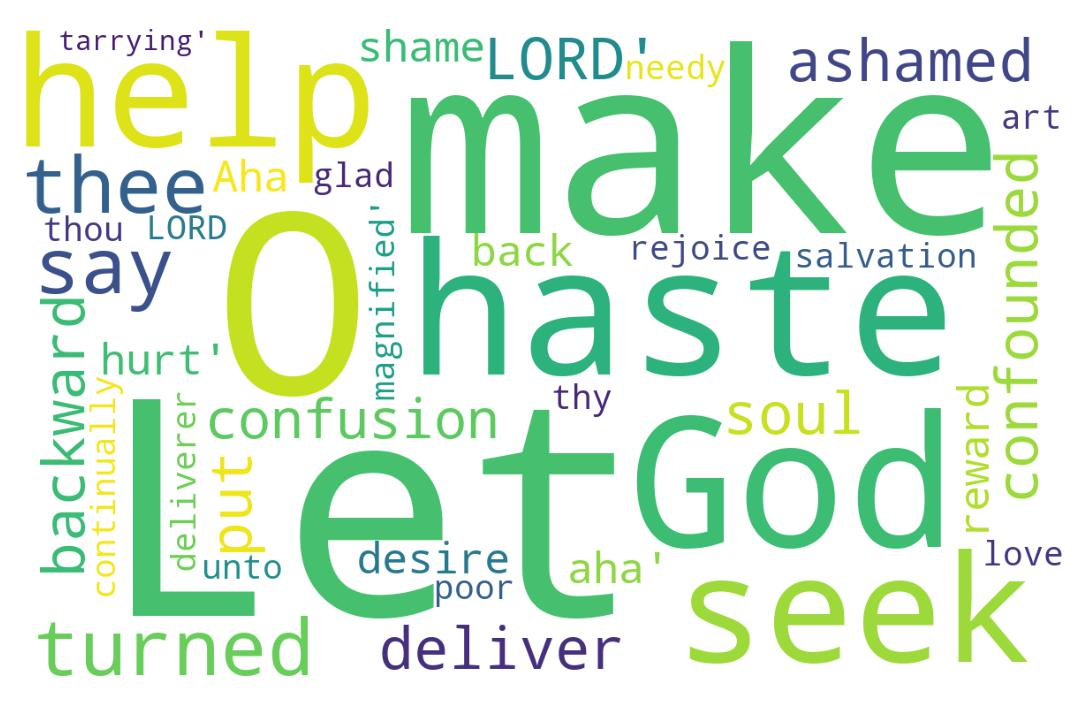
\includegraphics[width=\linewidth]{19OT-Psalms/Psalm70-WordCloud.jpg}
  \caption{Psalm 70 Word Cloud}
  \label{fig:Psalm 70 word Cloud}
\end{figure}



% \textcolor[cmyk]{0.99998,1,0,0}{
\marginpar{\scriptsize \centering \fcolorbox{bone}{lime}{\textbf{DAVID'S EMERGENCY PRAYER}}\\ (Psalm 70) \begin{compactenum}[I.][8]

     \item The \textbf{Distress} \index[scripture]{Psalms!Psa 070:01}(Psa 70:1)
    \item David's \textbf{Determination} \index[scripture]{Psalms!Psa 070:01}(Psa 70:1)
    \item The \textbf{Desire} of the Wicked\index[scripture]{Psalms!Psa 070:02}(Psa 70:2)
    \item Two \textbf{Different} Groups of People \index[scripture]{Psalms!Psa 070:03}\index[scripture]{Psalms!Psa 070:04}(Psa 70:3, 4)
    \item A \textbf{Declaration} \index[scripture]{Psalms!Psa 070:04}(Psa 70:4)
    \item The \textbf{Deliverer} \index[scripture]{Psalms!Psa 070:05}(Psa 70:5)
    \item A \textbf{Dependence} \index[scripture]{Psalms!Psa 070:05}(Psa 70:5)
\end{compactenum}}




\footnote{\textcolor[rgb]{0.00,0.25,0.00}{\hyperlink{TOC}{Return to end of Table of Contents.}}}\footnote{\href{https://audiobible.com/bible/psalms_70.html}{\textcolor[cmyk]{0.99998,1,0,0}{Psalm 70 Audio}}}\textcolor[cmyk]{0.99998,1,0,0}{To the chief Musician, \emph{A Psalm} of David, to bring to remembrance.}\\
\\
\textcolor[cmyk]{0.99998,1,0,0}{\emph{Make} \emph{haste}, O God, to deliver me; make haste to help me, O LORD.}
[2] \textcolor[cmyk]{0.99998,1,0,0}{Let them be ashamed and confounded that seek after my soul: let them be turned backward, and put to confusion, that desire my hurt.}
[3] \textcolor[cmyk]{0.99998,1,0,0}{Let them be turned back for a reward of their shame that say, Aha, aha.}
[4] \textcolor[cmyk]{0.99998,1,0,0}{Let all those that seek thee rejoice and be glad in thee: and let such as love thy salvation say continually, Let God be magnified.}
[5] \textcolor[cmyk]{0.99998,1,0,0}{But I \emph{am} poor and needy: make haste unto me, O God: thou \emph{art} my help and my deliverer; O LORD, make no tarrying.}







\index[NWIV]{14!Psalms!Psa 70:1}\index[AWIP]{\emph{Make}!Psalms!Psa 70:1}\index[AWIP]{\emph{haste}!Psalms!Psa 70:1}\index[AWIP]{O!Psalms!Psa 70:1}\index[AWIP]{O!Psalms!Psa 70:1 (2)}\index[AWIP]{God!Psalms!Psa 70:1}\index[AWIP]{to!Psalms!Psa 70:1}\index[AWIP]{to!Psalms!Psa 70:1 (2)}\index[AWIP]{deliver!Psalms!Psa 70:1}\index[AWIP]{me!Psalms!Psa 70:1}\index[AWIP]{me!Psalms!Psa 70:1 (2)}\index[AWIP]{make!Psalms!Psa 70:1}\index[AWIP]{haste!Psalms!Psa 70:1}\index[AWIP]{help!Psalms!Psa 70:1}\index[AWIP]{LORD!Psalms!Psa 70:1}\index[AWIP]{\emph{Make}!Psalms!Psa 70:1}\index[AWIP]{\emph{haste}!Psalms!Psa 70:1}

\index[NWIV]{24!Psalms!Psa 70:2}\index[AWIP]{Let!Psalms!Psa 70:2}\index[AWIP]{them!Psalms!Psa 70:2}\index[AWIP]{them!Psalms!Psa 70:2 (2)}\index[AWIP]{be!Psalms!Psa 70:2}\index[AWIP]{be!Psalms!Psa 70:2 (2)}\index[AWIP]{ashamed!Psalms!Psa 70:2}\index[AWIP]{and!Psalms!Psa 70:2}\index[AWIP]{and!Psalms!Psa 70:2 (2)}\index[AWIP]{confounded!Psalms!Psa 70:2}\index[AWIP]{that!Psalms!Psa 70:2}\index[AWIP]{that!Psalms!Psa 70:2 (2)}\index[AWIP]{seek!Psalms!Psa 70:2}\index[AWIP]{after!Psalms!Psa 70:2}\index[AWIP]{my!Psalms!Psa 70:2}\index[AWIP]{my!Psalms!Psa 70:2 (2)}\index[AWIP]{soul!Psalms!Psa 70:2}\index[AWIP]{let!Psalms!Psa 70:2}\index[AWIP]{turned!Psalms!Psa 70:2}\index[AWIP]{backward!Psalms!Psa 70:2}\index[AWIP]{put!Psalms!Psa 70:2}\index[AWIP]{to!Psalms!Psa 70:2}\index[AWIP]{confusion!Psalms!Psa 70:2}\index[AWIP]{desire!Psalms!Psa 70:2}\index[AWIP]{hurt!Psalms!Psa 70:2}

\index[NWIV]{15!Psalms!Psa 70:3}\index[AWIP]{Let!Psalms!Psa 70:3}\index[AWIP]{them!Psalms!Psa 70:3}\index[AWIP]{be!Psalms!Psa 70:3}\index[AWIP]{turned!Psalms!Psa 70:3}\index[AWIP]{back!Psalms!Psa 70:3}\index[AWIP]{for!Psalms!Psa 70:3}\index[AWIP]{a!Psalms!Psa 70:3}\index[AWIP]{reward!Psalms!Psa 70:3}\index[AWIP]{of!Psalms!Psa 70:3}\index[AWIP]{their!Psalms!Psa 70:3}\index[AWIP]{shame!Psalms!Psa 70:3}\index[AWIP]{that!Psalms!Psa 70:3}\index[AWIP]{say!Psalms!Psa 70:3}\index[AWIP]{Aha!Psalms!Psa 70:3}\index[AWIP]{aha!Psalms!Psa 70:3}

\index[NWIV]{25!Psalms!Psa 70:4}\index[AWIP]{Let!Psalms!Psa 70:4}\index[AWIP]{Let!Psalms!Psa 70:4 (2)}\index[AWIP]{all!Psalms!Psa 70:4}\index[AWIP]{those!Psalms!Psa 70:4}\index[AWIP]{that!Psalms!Psa 70:4}\index[AWIP]{seek!Psalms!Psa 70:4}\index[AWIP]{thee!Psalms!Psa 70:4}\index[AWIP]{thee!Psalms!Psa 70:4 (2)}\index[AWIP]{rejoice!Psalms!Psa 70:4}\index[AWIP]{and!Psalms!Psa 70:4}\index[AWIP]{and!Psalms!Psa 70:4 (2)}\index[AWIP]{be!Psalms!Psa 70:4}\index[AWIP]{be!Psalms!Psa 70:4 (2)}\index[AWIP]{glad!Psalms!Psa 70:4}\index[AWIP]{in!Psalms!Psa 70:4}\index[AWIP]{let!Psalms!Psa 70:4}\index[AWIP]{such!Psalms!Psa 70:4}\index[AWIP]{as!Psalms!Psa 70:4}\index[AWIP]{love!Psalms!Psa 70:4}\index[AWIP]{thy!Psalms!Psa 70:4}\index[AWIP]{salvation!Psalms!Psa 70:4}\index[AWIP]{say!Psalms!Psa 70:4}\index[AWIP]{continually!Psalms!Psa 70:4}\index[AWIP]{God!Psalms!Psa 70:4}\index[AWIP]{magnified!Psalms!Psa 70:4}

\index[NWIV]{24!Psalms!Psa 70:5}\index[AWIP]{But!Psalms!Psa 70:5}\index[AWIP]{I!Psalms!Psa 70:5}\index[AWIP]{\emph{am}!Psalms!Psa 70:5}\index[AWIP]{poor!Psalms!Psa 70:5}\index[AWIP]{and!Psalms!Psa 70:5}\index[AWIP]{and!Psalms!Psa 70:5 (2)}\index[AWIP]{needy!Psalms!Psa 70:5}\index[AWIP]{make!Psalms!Psa 70:5}\index[AWIP]{make!Psalms!Psa 70:5 (2)}\index[AWIP]{haste!Psalms!Psa 70:5}\index[AWIP]{unto!Psalms!Psa 70:5}\index[AWIP]{me!Psalms!Psa 70:5}\index[AWIP]{O!Psalms!Psa 70:5}\index[AWIP]{O!Psalms!Psa 70:5 (2)}\index[AWIP]{God!Psalms!Psa 70:5}\index[AWIP]{thou!Psalms!Psa 70:5}\index[AWIP]{\emph{art}!Psalms!Psa 70:5}\index[AWIP]{my!Psalms!Psa 70:5}\index[AWIP]{my!Psalms!Psa 70:5 (2)}\index[AWIP]{help!Psalms!Psa 70:5}\index[AWIP]{deliverer!Psalms!Psa 70:5}\index[AWIP]{LORD!Psalms!Psa 70:5}\index[AWIP]{no!Psalms!Psa 70:5}\index[AWIP]{tarrying!Psalms!Psa 70:5}\index[AWIP]{\emph{am}!Psalms!Psa 70:5}\index[AWIP]{\emph{art}!Psalms!Psa 70:5}


\section{Psalm 70 Outlines}

\subsection{My Outlines}

\subsubsection{David's Emergency Prayer}
\textbf{Introduction:} Compare with Psalm 40:13-17%\footnote{14 Augsut 2016, Keith Anthony.}
\index[speaker]{Keith Anthony!Psalm 070 (David's Emergency Prayer)}
\index[series]{Psalms (Keith Anthony)!Psalm 070 (David's Emergency Prayer)}
\index[date]{2016/08/14!Psalm 070 (David's Emergency Prayer) (Keith Anthony)}
\begin{compactenum}[I.]
    \item The \textbf{Distress} \index[scripture]{Psalms!Psa 070:01}(Psa 70:1)
    \item David's \textbf{Determination} \index[scripture]{Psalms!Psa 070:01}(Psa 70:1)
    \item The \textbf{Desire} of the Wicked\index[scripture]{Psalms!Psa 070:02}(Psa 70:2)
    \item Two \textbf{Different} Groups of People \index[scripture]{Psalms!Psa 070:03}\index[scripture]{Psalms!Psa 070:04}(Psa 70:3, 4)
    \item A \textbf{Declaration} \index[scripture]{Psalms!Psa 070:04}(Psa 70:4)
    \item The \textbf{Deliverer} \index[scripture]{Psalms!Psa 070:05}(Psa 70:5)
    \item A \textbf{Dependence} \index[scripture]{Psalms!Psa 070:05}(Psa 70:5)
\end{compactenum}


\subsection{Outlines from Others}


\section{Psalm 70 Comments}




\newpage
\subsection{Psalm70 Repeated Phrases}


%%%%%%%%%%
%%%%%%%%%%
\normalsize
 
\begin{center}
\begin{longtable}{|p{3.0in}|p{0.5in}|}
\caption[Psalm70 Repeated Phrases]{Psalm70 Repeated Phrases}\label{table:Repeated Phrases Psalm70} \\
\hline \multicolumn{1}{|c|}{\textbf{Phrase}} & \multicolumn{1}{c|}{\textbf{Frequency}} \\ \hline 
\endfirsthead
 
\multicolumn{2}{c}
{{\bfseries \tablename\ \thetable{} -- continued from previous page}} \\  
\hline \multicolumn{1}{|c|}{\textbf{Phrase}} & \multicolumn{1}{c|}{\textbf{Frequency}} \\ \hline 
\endhead
 
\hline \multicolumn{2}{c}{{ }} \\ \hline
\endfoot 
them be & 3\\ \hline 
\end{longtable}
\end{center}



%%%%%%%%%%
%%%%%%%%%%



\section{Psalm 70 Word Statistics}


%%%%%%%%%%
%%%%%%%%%%
\normalsize
 
\begin{center}
\begin{longtable}{l|c|c|c|c}
\caption[Psalm 70 Statistics]{Psalm 70 Statistics}\label{table:Statistics for Psalm 70} \\
\hline \multicolumn{1}{|c|}{\textbf{Verse(s)}} & \multicolumn{1}{|c|}{\textbf{Count}} & \multicolumn{1}{|c|}{\textbf{Unique}} & \multicolumn{1}{|c|}{\textbf{Italics}} & \multicolumn{1}{|c|}{\textbf{Uniq Italic}}  \\ \hline 
\endfirsthead
 
\multicolumn{5}{c}
{{\bfseries \tablename\ \thetable{} -- continued from previous page}} \\  
\hline \multicolumn{1}{|c|}{\textbf{Verse(s)}} & \multicolumn{1}{|c|}{\textbf{Count}} & \multicolumn{1}{|c|}{\textbf{Unique}} & \multicolumn{1}{|c|}{\textbf{Italics}} & \multicolumn{1}{|c|}{\textbf{Uniq Italic}}  \\ \hline 
\endhead
 
\hline \multicolumn{5}{|r|}{{Continued if needed}} \\ \hline
\endfoot 
1 & 14 & 11 & 2 & 2\\ \hline
2 & 24 & 19 & 0 & 0\\ \hline
3 & 15 & 15 & 0 & 0\\ \hline
4 & 25 & 21 & 0 & 0\\ \hline
5 & 24 & 20 & 2 & 2\\ \hline
Total & 102 & 63 & 4 & 4
\end{longtable}
\end{center}



%%%%%%%%%%
%%%%%%%%%%


\subsection{Psalm 70 Words by Frequency}


%%%%%%%%%%
%%%%%%%%%%
\normalsize
 
\begin{center}
\begin{longtable}{l|r}
\caption[Psalm 70 Words by Frequency]{Psalm 70 Words by Frequency}\label{table:WordsbyFrequency for Psalm 70} \\
\hline \multicolumn{1}{|c|}{\textbf{Word}} & \multicolumn{1}{c|}{\textbf{Frequency}} \\ \hline 
\endfirsthead
 
\multicolumn{2}{c}
{{\bfseries \tablename\ \thetable{} -- continued from previous page}} \\  
\hline \multicolumn{1}{|c|}{\textbf{Word}} & \multicolumn{1}{c|}{\textbf{Frequency}} \\ \hline 
\endhead
 
\hline \multicolumn{2}{c}{{ }} \\ \hline
\endfoot 
and & 6\\ \hline 
be & 5\\ \hline 
O & 4\\ \hline 
Let & 4\\ \hline 
that & 4\\ \hline 
my & 4\\ \hline 
God & 3\\ \hline 
to & 3\\ \hline 
me & 3\\ \hline 
make & 3\\ \hline 
them & 3\\ \hline 
haste & 2\\ \hline 
help & 2\\ \hline 
LORD & 2\\ \hline 
seek & 2\\ \hline 
let & 2\\ \hline 
turned & 2\\ \hline 
say & 2\\ \hline 
thee & 2\\ \hline 
\emph{Make} & 1\\ \hline 
\emph{haste} & 1\\ \hline 
deliver & 1\\ \hline 
ashamed & 1\\ \hline 
confounded & 1\\ \hline 
after & 1\\ \hline 
soul & 1\\ \hline 
backward & 1\\ \hline 
put & 1\\ \hline 
confusion & 1\\ \hline 
desire & 1\\ \hline 
hurt & 1\\ \hline 
back & 1\\ \hline 
for & 1\\ \hline 
a & 1\\ \hline 
reward & 1\\ \hline 
of & 1\\ \hline 
their & 1\\ \hline 
shame & 1\\ \hline 
Aha & 1\\ \hline 
aha & 1\\ \hline 
all & 1\\ \hline 
those & 1\\ \hline 
rejoice & 1\\ \hline 
glad & 1\\ \hline 
in & 1\\ \hline 
such & 1\\ \hline 
as & 1\\ \hline 
love & 1\\ \hline 
thy & 1\\ \hline 
salvation & 1\\ \hline 
continually & 1\\ \hline 
magnified & 1\\ \hline 
But & 1\\ \hline 
I & 1\\ \hline 
\emph{am} & 1\\ \hline 
poor & 1\\ \hline 
needy & 1\\ \hline 
unto & 1\\ \hline 
thou & 1\\ \hline 
\emph{art} & 1\\ \hline 
deliverer & 1\\ \hline 
no & 1\\ \hline 
tarrying & 1\\ \hline 
\end{longtable}
\end{center}



%%%%%%%%%%
%%%%%%%%%%


\subsection{Psalm 70 Words Alphabetically}


%%%%%%%%%%
%%%%%%%%%%
\normalsize
 
\begin{center}
\begin{longtable}{l|r}
\caption[Psalm 70 Words Alphabetically]{Psalm 70 Words Alphabetically}\label{table:WordsAlphabetically for Psalm 70} \\
\hline \multicolumn{1}{|c|}{\textbf{Word}} & \multicolumn{1}{c|}{\textbf{Frequency}} \\ \hline 
\endfirsthead
 
\multicolumn{2}{c}
{{\bfseries \tablename\ \thetable{} -- continued from previous page}} \\  
\hline \multicolumn{1}{|c|}{\textbf{Word}} & \multicolumn{1}{c|}{\textbf{Frequency}} \\ \hline 
\endhead
 
\hline \multicolumn{2}{c}{{ }} \\ \hline
\endfoot 
Aha & 1\\ \hline 
But & 1\\ \hline 
God & 3\\ \hline 
I & 1\\ \hline 
LORD & 2\\ \hline 
Let & 4\\ \hline 
O & 4\\ \hline 
\emph{Make} & 1\\ \hline 
\emph{am} & 1\\ \hline 
\emph{art} & 1\\ \hline 
\emph{haste} & 1\\ \hline 
a & 1\\ \hline 
after & 1\\ \hline 
aha & 1\\ \hline 
all & 1\\ \hline 
and & 6\\ \hline 
as & 1\\ \hline 
ashamed & 1\\ \hline 
back & 1\\ \hline 
backward & 1\\ \hline 
be & 5\\ \hline 
confounded & 1\\ \hline 
confusion & 1\\ \hline 
continually & 1\\ \hline 
deliver & 1\\ \hline 
deliverer & 1\\ \hline 
desire & 1\\ \hline 
for & 1\\ \hline 
glad & 1\\ \hline 
haste & 2\\ \hline 
help & 2\\ \hline 
hurt & 1\\ \hline 
in & 1\\ \hline 
let & 2\\ \hline 
love & 1\\ \hline 
magnified & 1\\ \hline 
make & 3\\ \hline 
me & 3\\ \hline 
my & 4\\ \hline 
needy & 1\\ \hline 
no & 1\\ \hline 
of & 1\\ \hline 
poor & 1\\ \hline 
put & 1\\ \hline 
rejoice & 1\\ \hline 
reward & 1\\ \hline 
salvation & 1\\ \hline 
say & 2\\ \hline 
seek & 2\\ \hline 
shame & 1\\ \hline 
soul & 1\\ \hline 
such & 1\\ \hline 
tarrying & 1\\ \hline 
that & 4\\ \hline 
thee & 2\\ \hline 
their & 1\\ \hline 
them & 3\\ \hline 
those & 1\\ \hline 
thou & 1\\ \hline 
thy & 1\\ \hline 
to & 3\\ \hline 
turned & 2\\ \hline 
unto & 1\\ \hline 
\end{longtable}
\end{center}



%%%%%%%%%%
%%%%%%%%%%


\subsection{Psalm 70 Words by Length}


%%%%%%%%%%
%%%%%%%%%%
\normalsize
 
\begin{center}
\begin{longtable}{l|p{3.75in}}
\caption[Psalm 70 Words by Length]{Psalm 70 Words by Length}\label{table:WordsAlphabetically for Psalm 70} \\
\hline \multicolumn{1}{|c|}{\textbf{Length}} & \multicolumn{1}{c|}{\textbf{Words}} \\ \hline 
\endfirsthead
\hline \multicolumn{1}{|c|}{\textbf{Length}} & \multicolumn{1}{c|}{\textbf{Words}} \\ \hline 
\multicolumn{2}{c}
{{\bfseries \tablename\ \thetable{} -- continued from previous page}} \\  
\hline \multicolumn{1}{|c|}{\textbf{Word}} & \multicolumn{1}{c|}{\textbf{Frequency}} \\ \hline 
\endhead
 
\hline \multicolumn{2}{c}{{ }} \\ \hline
\endfoot 
1 & O, a, I\\ \hline 
2 & to, me, be, my, of, in, as, \emph{am}, no\\ \hline 
3 & God, Let, and, let, put, for, say, Aha, aha, all, thy, But, \emph{art}\\ \hline 
4 & \emph{Make}, make, help, LORD, them, that, seek, soul, hurt, back, thee, glad, such, love, poor, unto, thou\\ \hline 
5 & \emph{haste}, haste, after, their, shame, those, needy\\ \hline 
6 & turned, desire, reward\\ \hline 
7 & deliver, ashamed, rejoice\\ \hline 
8 & backward, tarrying\\ \hline 
9 & confusion, salvation, magnified, deliverer\\ \hline 
10 & confounded\\ \hline 
11 & continually\\ \hline 
\end{longtable}
\end{center}



%%%%%%%%%%
%%%%%%%%%%




\chapter{Proverb 11}

\begin{figure}
  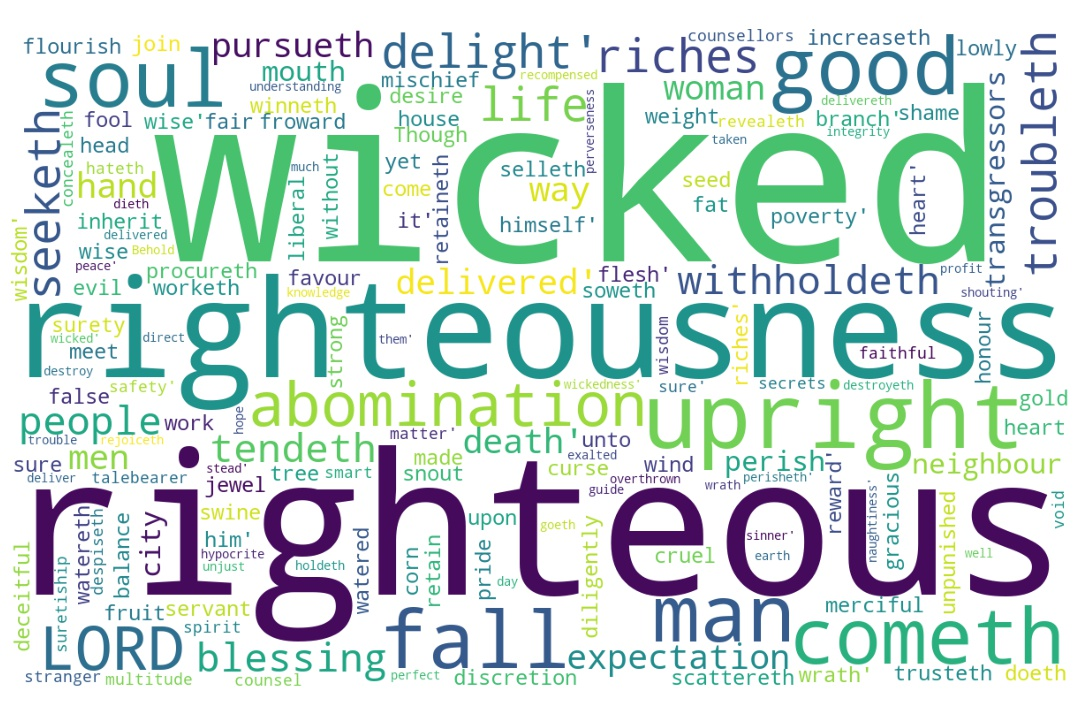
\includegraphics[width=\linewidth]{20OT-Proverbs/Proverb11-WordCloud.jpg}
  \caption{Proverb 11 Word Cloud}
  \label{fig:Proverb 11 Word Cloud}
\end{figure}

\marginpar{\scriptsize \centering \fcolorbox{bone}{lime}{\textbf{MISSING IMPORTANT THINGS}}\\ (Proverbs 11:1-31) \begin{compactenum}[I.][8]
    \item No \textbf{Balance} \index[scripture]{Proverbs!Pro 11:01} (Pro 11:1) 
    \item No \textbf{Integrity} \index[scripture]{Proverbs!Pro 11:03}(Pro 11:3) 
    \item No \textbf{Expectation} \index[scripture]{Proverbs!Pro 11:07}(Pro 11:7) 
    \item No \textbf{Wisdom} \index[scripture]{Proverbs!Pro 11:12}(Pro 11:12) 
    \item No \textbf{Counsel} \index[scripture]{Proverbs!Pro 11:14}(Pro 11:14) 
    \item No \textbf{Discretion} \index[scripture]{Proverbs!Pro 11:22}(Pro 11:22) 
    \item No \textbf{Corn (food)} \index[scripture]{Proverbs!Pro 11:26}(Pro 11:26) 
\end{compactenum}}

\marginpar{\scriptsize \centering \fcolorbox{bone}{yellow}{\textbf{UNDEPENDABLE}}\\ (Proverbs 11:1-31) \begin{compactenum}[I.][8]
    \item \textbf{Riches in the Day of Wrath} \index[scripture]{Proverbs!Pro 11:04}\index[scripture]{Proverbs!Pro 11:28}(Pro 11:4, 28)
    \item \textbf{A Hypocrite to Keep his Word} \index[scripture]{Proverbs!Pro 11:09}(Pro 11:9)
    \item \textbf{Mouth of the Wicked}\index[scripture]{Proverbs!Pro 11:11} (Pro 11:11)
    \item \textbf{A Foolish Neighbor Providing Wisdom} \index[scripture]{Proverbs!Pro 11:12}(Pro 11:12)
    \item \textbf{Lasting Blessing from a Deceitful Work} \index[scripture]{Proverbs!Pro 11:18}(Pro 11:18)
    \item \textbf{Discretion from an Evil Woman} \index[scripture]{Proverbs!Pro 11:22} (Pro 11:22)
    \item \textbf{A Fool to not Withhold}\index[scripture]{Proverbs!Pro 11:24}\index[scripture]{Proverbs!Pro 11:27} (Pro 11:24, 27)
\end{compactenum}}

\marginpar{\scriptsize \centering \fcolorbox{bone}{black}{\textbf{\textcolor[cmyk]{0,0,0,0}{WALKING THE RIGHT PATH}}}\\ (Proverbs 11) \begin{compactenum}[I.][8]
    \item The \textbf{Delight of the Lord} \index[scripture]{Proverbs!Pro 11:01}\index[scripture]{Proverbs!Pro 11:20}(Pro 11:1, 20)
     \item   \textbf{Deliverance} \index[scripture]{Proverbs!Pro 11:04}  \index[scripture]{Proverbs!Pro 11:06} \index[scripture]{Proverbs!Pro 11:08} \index[scripture]{Proverbs!Pro 11:09} \index[scripture]{Proverbs!Pro 11:21}(Pro 11:4, 6, 8, 9, 21)
     \item  A \textbf{Directing} \index[scripture]{Proverbs!Pro 11:05} (Pro 11:5)
   \item  \textbf{Discretion} \index[scripture]{Proverbs!Pro 11:22} (Pro 11:22)
   \item  \textbf{Desire} \index[scripture]{Proverbs!Pro 11:23} (Pro 11:23)
   \item  \textbf{Diligence} \index[scripture]{Proverbs!Pro 11:27} (Pro 11:27)
    \item  A \textbf{Destination} \index[scripture]{Proverbs!Pro 11:30} (Pro 11:30)
\end{compactenum}}

\marginpar{\scriptsize \centering 
\fcolorbox{black}{blue}{\textbf{\textcolor[cmyk]{0,0,0,0}{A PERSON OUT OF BALANCE}}}\\ 
(Proverbs 11:1) 
\begin{compactenum}[I.][8]
    \item \textbf{Tends to Fall a Lot}  
    \item \textbf{Breaks Things}
    \item \textbf{Bumps Into Things}  
    \item \textbf{Looks Funny or Foolish or Pathetic}
    \item \textbf{Usually Needs a Crutch}
    \item \textbf{Requires Extra Attention}
    \item \textbf{Throws off Judgment}
\end{compactenum}}




\footnote{\textcolor[cmyk]{0.99998,1,0,0}{\hyperlink{TOC}{Return to end of Table of Contents.}}}\footnote{\href{https://www.audioverse.org/english/audiobibles/books/ENGKJV/O/Prov/1}{\textcolor[cmyk]{0.99998,1,0,0}{Proverbs Audio}}}\textcolor[cmyk]{0.99998,1,0,0}{A \fcolorbox{bone}{lime}{false balance} \emph{is} abomination to the LORD: but \fcolorbox{bone}{bone}{a} just weight \emph{is} \fcolorbox{bone}{bone}{his} delight.}\footnote{\textbf{Proverb 16:11} - A just weight and balance are the LORD's: all the weights of the bag are his work.}\footnote{\textbf{Proverb 20:10} - Divers weights, and divers measures, both of them are alike abomination to the LORD.}\footnote{\textbf{Proverb 20:23} - Divers weights are an abomination unto the LORD; and a false balance is not good.}\footnote{\textbf{Ezekiel 45:10-12} - Ye shall have just balances, and a just ephah, and a just bath. [11] The ephah and the bath shall be of one measure, that the bath may contain the tenth part of an homer, and the ephah the tenth part of an homer: the measure thereof shall be after the homer. [12] And the shekel shall be twenty gerahs: twenty shekels, five and twenty shekels, fifteen shekels, shall be your maneh.}\footnote{\textbf{Hosea 12:7} - He is a merchant, the balances of deceit are in his hand: he loveth to oppress.}\footnote{\textbf{Amos 8:5-6} - Saying, When will the new moon be gone, that we may sell corn? and the sabbath, that we may set forth wheat, making the ephah small, and the shekel great, and falsifying the balances by deceit? That we may buy the poor for silver, and the needy for a pair of shoes; yea, and sell the refuse of the wheat?}\footnote{\textbf{Micah 6:10-11} - Are there yet the treasures of wickedness in the house of the wicked, and the scant measure that is abominable? Shall I count them pure with the wicked balances, and with the bag of deceitful weights?}
[2] \textcolor[cmyk]{0.99998,1,0,0}{\emph{When} pride cometh, then cometh shame: but with the lowly \emph{is} wisdom.}\footnote{\textbf{Proverb 16:18-19} - Pride goeth before destruction, and an haughty spirit before a fall. [19] Better it is to be of an humble spirit with the lowly, than to divide the spoil with the proud.}\footnote{\textbf{Daniel 4:30-32} - The king spake, and said, Is not this great Babylon, that I have built for the house of the kingdom by the might of my power, and for the honour of my majesty? [31] While the word was in the king's mouth, there fell a voice from heaven, saying, O king Nebuchadnezzar, to thee it is spoken; The kingdom is departed from thee. [32] And they shall drive thee from men, and thy dwelling shall be with the beasts of the field: they shall make thee to eat grass as oxen, and seven times shall pass over thee, until thou know that the most High ruleth in the kingdom of men, and giveth it to whomsoever he will.}\footnote{\textbf{Proverb 15:33} - The fear of the LORD is the instruction of wisdom; and before honour is humility.}\footnote{\textbf{1 Corinthians 8:1-2} - Now as touching things offered unto idols, we know that we all have knowledge. Knowledge puffeth up, but charity edifieth. [2] And if any man think that he knoweth any thing, he knoweth nothing yet as he ought to know.}
[3] \textcolor[cmyk]{0.99998,1,0,0}{The \fcolorbox{bone}{lime}{integrity} of the upright shall guide them: but the perverseness of \fcolorbox{bone}{MYGOLD}{transgressors} shall destroy them.}
[4] \textcolor[cmyk]{0.99998,1,0,0}{Riches profit not in the day of wrath: but \fcolorbox{bone}{MYGOLD}{righteousness} delivereth from death.}
[5] \textcolor[cmyk]{0.99998,1,0,0}{The \fcolorbox{bone}{MYGOLD}{righteousness} of the perfect shall direct \fcolorbox{bone}{bone}{his} way: but the wicked shall fall by \fcolorbox{bone}{bone}{his} own wickedness.}
[6] \textcolor[cmyk]{0.99998,1,0,0}{The \fcolorbox{bone}{MYGOLD}{righteousness} of the upright shall deliver them: but \fcolorbox{bone}{MYGOLD}{transgressors} shall be taken in \emph{their} \emph{own} naughtiness.}
[7] \textcolor[cmyk]{0.99998,1,0,0}{When \fcolorbox{bone}{bone}{a} wicked man dieth, \emph{his} \fcolorbox{bone}{lime}{expectation} shall perish: and the hope of unjust \emph{men} perisheth.}
[8] \textcolor[cmyk]{0.99998,1,0,0}{The righteous is delivered out of trouble, and the wicked cometh in \fcolorbox{bone}{bone}{his} stead.}
[9] \textcolor[cmyk]{0.99998,1,0,0}{An hypocrite with \emph{his} mouth destroyeth \fcolorbox{bone}{bone}{his} neighbour: but through knowledge shall the just be delivered.}
[10] \textcolor[cmyk]{0.99998,1,0,0}{When it goeth well with the righteous, the city rejoiceth: and when the wicked perish, \emph{there} \emph{is} shouting.}
[11] \textcolor[cmyk]{0.99998,1,0,0}{By the blessing of the upright the city is exalted: but it is overthrown by the mouth of the wicked.}
[12] \textcolor[cmyk]{0.99998,1,0,0}{He that is void of \fcolorbox{bone}{lime}{wisdom} despiseth \fcolorbox{bone}{bone}{his} neighbour: but \fcolorbox{bone}{bone}{a} man of \fcolorbox{bone}{MYGOLD}{understanding} holdeth \fcolorbox{bone}{bone}{his} peace.}
[13] \textcolor[cmyk]{0.99998,1,0,0}{A talebearer revealeth secrets: but he that is of \fcolorbox{bone}{bone}{a} faithful spirit concealeth the matter.}
[14] \textcolor[cmyk]{0.99998,1,0,0}{Where \fcolorbox{bone}{lime}{no counsel} \emph{is}, the people fall: but in the multitude of counsellors \emph{there} \emph{is} safety.}\footnote{\textbf{Proverb 15:22} - Without counsel purposes are disappointed: but in the multitude of counsellors they are established.}\footnote{\textbf{Proverb 16:22} - Understanding is a wellspring of life unto him that hath it: but the instruction of fools is folly.}\footnote{\textbf{Proverb 24:6} - For by wise counsel thou shalt make thy war: and in multitude of counsellors there is safety.}
[15] \textcolor[cmyk]{0.99998,1,0,0}{He that is surety for \fcolorbox{bone}{bone}{a} stranger shall smart \emph{for} \emph{it}: and he that hateth suretiship is sure.}\footnote{\textbf{Proverb 6:1-5} - My son, if thou be surety for thy friend, if thou hast stricken thy hand with a stranger, [2] Thou art snared with the words of thy mouth, thou art taken with the words of thy mouth. [3] Do this now, my son, and deliver thyself, when thou art come into the hand of thy friend; go, humble thyself, and make sure thy friend. [4] Give not sleep to thine eyes, nor slumber to thine eyelids. [5] Deliver thyself as a roe from the hand of the hunter, and as a bird from the hand of the fowler.}
[16] \textcolor[cmyk]{0.99998,1,0,0}{A gracious woman retaineth honour: and strong \emph{men} retain riches.}
[17] \textcolor[cmyk]{0.99998,1,0,0}{The merciful man doeth good to \fcolorbox{bone}{bone}{his} own soul: but \emph{he} \emph{that} \emph{is} cruel troubleth \fcolorbox{bone}{bone}{his} own flesh.}
[18] \textcolor[cmyk]{0.99998,1,0,0}{The wicked worketh \fcolorbox{bone}{bone}{a} deceitful work: but to him that soweth \fcolorbox{bone}{MYGOLD}{righteousness} \emph{shall} \emph{be} \fcolorbox{bone}{bone}{a} sure reward.}
[19] \textcolor[cmyk]{0.99998,1,0,0}{As \fcolorbox{bone}{MYGOLD}{righteousness} \emph{tendeth} to life: so he that pursueth evil \emph{pursueth} \emph{it} to \fcolorbox{bone}{bone}{his} own death.}
[20] \textcolor[cmyk]{0.99998,1,0,0}{They that are of \fcolorbox{bone}{bone}{a} froward heart \emph{are} abomination to the LORD: but \emph{such} \emph{as} \emph{are} upright in \emph{their} way \emph{are} \fcolorbox{bone}{bone}{his} delight.}
[21] \textcolor[cmyk]{0.99998,1,0,0}{\emph{Though} hand \emph{join} in hand, the wicked shall not be unpunished: but the seed of the righteous shall be delivered.}
[22] \textcolor[cmyk]{0.99998,1,0,0}{\emph{As} a jewel of gold in \fcolorbox{bone}{bone}{a} swine's snout, \emph{so} \emph{is} \fcolorbox{bone}{bone}{a} fair woman which is without \fcolorbox{bone}{lime}{discretion}.}
[23] \textcolor[cmyk]{0.99998,1,0,0}{The desire of the righteous \emph{is} only good: \emph{but} the expectation of the wicked \emph{is} wrath.}
[24] \textcolor[cmyk]{0.99998,1,0,0}{There is that scattereth, and yet increaseth; and \emph{there} \emph{is} that withholdeth more than is meet, but \emph{it} \emph{tendeth} to poverty.}
[25] \textcolor[cmyk]{0.99998,1,0,0}{The liberal soul shall be made fat: and he that watereth shall be watered also himself.}
[26] \textcolor[cmyk]{0.99998,1,0,0}{He that \fcolorbox{bone}{lime}{withholdeth corn}, the people shall curse him: but blessing \emph{shall} \emph{be} upon the head of him that selleth \emph{it}.}
[27] \textcolor[cmyk]{0.99998,1,0,0}{He that diligently seeketh good procureth favour: but he that seeketh mischief, it shall come unto him.}
[28] \textcolor[cmyk]{0.99998,1,0,0}{He that trusteth in \fcolorbox{bone}{bone}{his} riches shall fall: but the righteous shall flourish as \fcolorbox{bone}{bone}{a} branch.}
[29] \textcolor[cmyk]{0.99998,1,0,0}{He that troubleth \fcolorbox{bone}{bone}{his} own house shall inherit the wind: and the fool \emph{shall} \emph{be} servant to the wise of heart.}\footnote{\textbf{1 Samuel 25:3, 17, 38} - Now the name of the man was Nabal; and the name of his wife Abigail: and she was a woman of good understanding, and of a beautiful countenance: but the man was churlish and evil in his doings; and he was of the house of Caleb. [17] Now therefore know and consider what thou wilt do; for evil is determined against our master, and against all his household: for he is such a son of Belial, that a man cannot speak to him. [38] And it came to pass about ten days after, that the LORD smote Nabal, that he died.}\footnote{\textbf{Hosea 8:7} - For they have sown the wind, and they shall reap the whirlwind: it hath no stalk: the bud shall yield no meal: if so be it yield, the strangers shall swallow it up.}
[30] \textcolor[cmyk]{0.99998,1,0,0}{The fruit of the righteous \emph{is} \fcolorbox{bone}{bone}{a} tree of life; and he that winneth souls \emph{is} wise.}\footnote{\textbf{Proverb 3:18} - She is a tree of life to them that lay hold upon her: and happy is every one that retaineth her.}\footnote{\textbf{Proverb 15:4} -A wholesome tongue is a tree of life: but perverseness therein is a breach in the spirit.}\footnote{\textbf{Daniel 12:3} - And they that be wise shall shine as the brightness of the firmament; and they that turn many to righteousness as the stars for ever and ever.}\footnote{\textbf{James 5:20} - Let him know, that he which converteth the sinner from the error of his way shall save a soul from death, and shall hide a multitude of sins.}
[31] \textcolor[cmyk]{0.99998,1,0,0}{Behold, the righteous shall be recompensed in the earth: much more the wicked and the sinner.}

\index[NWIV]{15!Proverbs!Pro 11:1}\index[AWIP]{A!Proverbs!Pro 11:1}\index[AWIP]{false!Proverbs!Pro 11:1}\index[AWIP]{balance!Proverbs!Pro 11:1}\index[AWIP]{\emph{is}!Proverbs!Pro 11:1}\index[AWIP]{\emph{is}!Proverbs!Pro 11:1 (2)}\index[AWIP]{abomination!Proverbs!Pro 11:1}\index[AWIP]{to!Proverbs!Pro 11:1}\index[AWIP]{the!Proverbs!Pro 11:1}\index[AWIP]{LORD!Proverbs!Pro 11:1}\index[AWIP]{but!Proverbs!Pro 11:1}\index[AWIP]{a!Proverbs!Pro 11:1}\index[AWIP]{just!Proverbs!Pro 11:1}\index[AWIP]{weight!Proverbs!Pro 11:1}\index[AWIP]{his!Proverbs!Pro 11:1}\index[AWIP]{delight!Proverbs!Pro 11:1}\index[AWIP]{\emph{is}!Proverbs!Pro 11:1}\index[AWIP]{\emph{is}!Proverbs!Pro 11:1 (2)}

\index[NWIV]{12!Proverbs!Pro 11:2}\index[AWIP]{\emph{When}!Proverbs!Pro 11:2}\index[AWIP]{pride!Proverbs!Pro 11:2}\index[AWIP]{cometh!Proverbs!Pro 11:2}\index[AWIP]{cometh!Proverbs!Pro 11:2 (2)}\index[AWIP]{then!Proverbs!Pro 11:2}\index[AWIP]{shame!Proverbs!Pro 11:2}\index[AWIP]{but!Proverbs!Pro 11:2}\index[AWIP]{with!Proverbs!Pro 11:2}\index[AWIP]{the!Proverbs!Pro 11:2}\index[AWIP]{lowly!Proverbs!Pro 11:2}\index[AWIP]{\emph{is}!Proverbs!Pro 11:2}\index[AWIP]{wisdom!Proverbs!Pro 11:2}\index[AWIP]{\emph{When}!Proverbs!Pro 11:2}\index[AWIP]{\emph{is}!Proverbs!Pro 11:2}

\index[NWIV]{16!Proverbs!Pro 11:3}\index[AWIP]{The!Proverbs!Pro 11:3}\index[AWIP]{integrity!Proverbs!Pro 11:3}\index[AWIP]{of!Proverbs!Pro 11:3}\index[AWIP]{of!Proverbs!Pro 11:3 (2)}\index[AWIP]{the!Proverbs!Pro 11:3}\index[AWIP]{the!Proverbs!Pro 11:3 (2)}\index[AWIP]{upright!Proverbs!Pro 11:3}\index[AWIP]{shall!Proverbs!Pro 11:3}\index[AWIP]{shall!Proverbs!Pro 11:3 (2)}\index[AWIP]{guide!Proverbs!Pro 11:3}\index[AWIP]{them!Proverbs!Pro 11:3}\index[AWIP]{them!Proverbs!Pro 11:3 (2)}\index[AWIP]{but!Proverbs!Pro 11:3}\index[AWIP]{perverseness!Proverbs!Pro 11:3}\index[AWIP]{transgressors!Proverbs!Pro 11:3}\index[AWIP]{destroy!Proverbs!Pro 11:3}

\index[NWIV]{13!Proverbs!Pro 11:4}\index[AWIP]{Riches!Proverbs!Pro 11:4}\index[AWIP]{profit!Proverbs!Pro 11:4}\index[AWIP]{not!Proverbs!Pro 11:4}\index[AWIP]{in!Proverbs!Pro 11:4}\index[AWIP]{the!Proverbs!Pro 11:4}\index[AWIP]{day!Proverbs!Pro 11:4}\index[AWIP]{of!Proverbs!Pro 11:4}\index[AWIP]{wrath!Proverbs!Pro 11:4}\index[AWIP]{but!Proverbs!Pro 11:4}\index[AWIP]{righteousness!Proverbs!Pro 11:4}\index[AWIP]{delivereth!Proverbs!Pro 11:4}\index[AWIP]{from!Proverbs!Pro 11:4}\index[AWIP]{death!Proverbs!Pro 11:4}

\index[NWIV]{18!Proverbs!Pro 11:5}\index[AWIP]{The!Proverbs!Pro 11:5}\index[AWIP]{righteousness!Proverbs!Pro 11:5}\index[AWIP]{of!Proverbs!Pro 11:5}\index[AWIP]{the!Proverbs!Pro 11:5}\index[AWIP]{the!Proverbs!Pro 11:5 (2)}\index[AWIP]{perfect!Proverbs!Pro 11:5}\index[AWIP]{shall!Proverbs!Pro 11:5}\index[AWIP]{shall!Proverbs!Pro 11:5 (2)}\index[AWIP]{direct!Proverbs!Pro 11:5}\index[AWIP]{his!Proverbs!Pro 11:5}\index[AWIP]{his!Proverbs!Pro 11:5 (2)}\index[AWIP]{way!Proverbs!Pro 11:5}\index[AWIP]{but!Proverbs!Pro 11:5}\index[AWIP]{wicked!Proverbs!Pro 11:5}\index[AWIP]{fall!Proverbs!Pro 11:5}\index[AWIP]{by!Proverbs!Pro 11:5}\index[AWIP]{own!Proverbs!Pro 11:5}\index[AWIP]{wickedness!Proverbs!Pro 11:5}

\index[NWIV]{17!Proverbs!Pro 11:6}\index[AWIP]{The!Proverbs!Pro 11:6}\index[AWIP]{righteousness!Proverbs!Pro 11:6}\index[AWIP]{of!Proverbs!Pro 11:6}\index[AWIP]{the!Proverbs!Pro 11:6}\index[AWIP]{upright!Proverbs!Pro 11:6}\index[AWIP]{shall!Proverbs!Pro 11:6}\index[AWIP]{shall!Proverbs!Pro 11:6 (2)}\index[AWIP]{deliver!Proverbs!Pro 11:6}\index[AWIP]{them!Proverbs!Pro 11:6}\index[AWIP]{but!Proverbs!Pro 11:6}\index[AWIP]{transgressors!Proverbs!Pro 11:6}\index[AWIP]{be!Proverbs!Pro 11:6}\index[AWIP]{taken!Proverbs!Pro 11:6}\index[AWIP]{in!Proverbs!Pro 11:6}\index[AWIP]{\emph{their}!Proverbs!Pro 11:6}\index[AWIP]{\emph{own}!Proverbs!Pro 11:6}\index[AWIP]{naughtiness!Proverbs!Pro 11:6}\index[AWIP]{\emph{their}!Proverbs!Pro 11:6}\index[AWIP]{\emph{own}!Proverbs!Pro 11:6}

\index[NWIV]{16!Proverbs!Pro 11:7}\index[AWIP]{When!Proverbs!Pro 11:7}\index[AWIP]{a!Proverbs!Pro 11:7}\index[AWIP]{wicked!Proverbs!Pro 11:7}\index[AWIP]{man!Proverbs!Pro 11:7}\index[AWIP]{dieth!Proverbs!Pro 11:7}\index[AWIP]{\emph{his}!Proverbs!Pro 11:7}\index[AWIP]{expectation!Proverbs!Pro 11:7}\index[AWIP]{shall!Proverbs!Pro 11:7}\index[AWIP]{perish!Proverbs!Pro 11:7}\index[AWIP]{and!Proverbs!Pro 11:7}\index[AWIP]{the!Proverbs!Pro 11:7}\index[AWIP]{hope!Proverbs!Pro 11:7}\index[AWIP]{of!Proverbs!Pro 11:7}\index[AWIP]{unjust!Proverbs!Pro 11:7}\index[AWIP]{\emph{men}!Proverbs!Pro 11:7}\index[AWIP]{perisheth!Proverbs!Pro 11:7}\index[AWIP]{\emph{his}!Proverbs!Pro 11:7}\index[AWIP]{\emph{men}!Proverbs!Pro 11:7}

\index[NWIV]{14!Proverbs!Pro 11:8}\index[AWIP]{The!Proverbs!Pro 11:8}\index[AWIP]{righteous!Proverbs!Pro 11:8}\index[AWIP]{is!Proverbs!Pro 11:8}\index[AWIP]{delivered!Proverbs!Pro 11:8}\index[AWIP]{out!Proverbs!Pro 11:8}\index[AWIP]{of!Proverbs!Pro 11:8}\index[AWIP]{trouble!Proverbs!Pro 11:8}\index[AWIP]{and!Proverbs!Pro 11:8}\index[AWIP]{the!Proverbs!Pro 11:8}\index[AWIP]{wicked!Proverbs!Pro 11:8}\index[AWIP]{cometh!Proverbs!Pro 11:8}\index[AWIP]{in!Proverbs!Pro 11:8}\index[AWIP]{his!Proverbs!Pro 11:8}\index[AWIP]{stead!Proverbs!Pro 11:8}

\index[NWIV]{16!Proverbs!Pro 11:9}\index[AWIP]{An!Proverbs!Pro 11:9}\index[AWIP]{hypocrite!Proverbs!Pro 11:9}\index[AWIP]{with!Proverbs!Pro 11:9}\index[AWIP]{\emph{his}!Proverbs!Pro 11:9}\index[AWIP]{mouth!Proverbs!Pro 11:9}\index[AWIP]{destroyeth!Proverbs!Pro 11:9}\index[AWIP]{his!Proverbs!Pro 11:9}\index[AWIP]{neighbour!Proverbs!Pro 11:9}\index[AWIP]{but!Proverbs!Pro 11:9}\index[AWIP]{through!Proverbs!Pro 11:9}\index[AWIP]{knowledge!Proverbs!Pro 11:9}\index[AWIP]{shall!Proverbs!Pro 11:9}\index[AWIP]{the!Proverbs!Pro 11:9}\index[AWIP]{just!Proverbs!Pro 11:9}\index[AWIP]{be!Proverbs!Pro 11:9}\index[AWIP]{delivered!Proverbs!Pro 11:9}\index[AWIP]{\emph{his}!Proverbs!Pro 11:9}

\index[NWIV]{18!Proverbs!Pro 11:10}\index[AWIP]{When!Proverbs!Pro 11:10}\index[AWIP]{it!Proverbs!Pro 11:10}\index[AWIP]{goeth!Proverbs!Pro 11:10}\index[AWIP]{well!Proverbs!Pro 11:10}\index[AWIP]{with!Proverbs!Pro 11:10}\index[AWIP]{the!Proverbs!Pro 11:10}\index[AWIP]{the!Proverbs!Pro 11:10 (2)}\index[AWIP]{the!Proverbs!Pro 11:10 (3)}\index[AWIP]{righteous!Proverbs!Pro 11:10}\index[AWIP]{city!Proverbs!Pro 11:10}\index[AWIP]{rejoiceth!Proverbs!Pro 11:10}\index[AWIP]{and!Proverbs!Pro 11:10}\index[AWIP]{when!Proverbs!Pro 11:10}\index[AWIP]{wicked!Proverbs!Pro 11:10}\index[AWIP]{perish!Proverbs!Pro 11:10}\index[AWIP]{\emph{there}!Proverbs!Pro 11:10}\index[AWIP]{\emph{is}!Proverbs!Pro 11:10}\index[AWIP]{shouting!Proverbs!Pro 11:10}\index[AWIP]{\emph{there}!Proverbs!Pro 11:10}\index[AWIP]{\emph{is}!Proverbs!Pro 11:10}

\index[NWIV]{20!Proverbs!Pro 11:11}\index[AWIP]{By!Proverbs!Pro 11:11}\index[AWIP]{the!Proverbs!Pro 11:11}\index[AWIP]{the!Proverbs!Pro 11:11 (2)}\index[AWIP]{the!Proverbs!Pro 11:11 (3)}\index[AWIP]{the!Proverbs!Pro 11:11 (4)}\index[AWIP]{the!Proverbs!Pro 11:11 (5)}\index[AWIP]{blessing!Proverbs!Pro 11:11}\index[AWIP]{of!Proverbs!Pro 11:11}\index[AWIP]{of!Proverbs!Pro 11:11 (2)}\index[AWIP]{upright!Proverbs!Pro 11:11}\index[AWIP]{city!Proverbs!Pro 11:11}\index[AWIP]{is!Proverbs!Pro 11:11}\index[AWIP]{is!Proverbs!Pro 11:11 (2)}\index[AWIP]{exalted!Proverbs!Pro 11:11}\index[AWIP]{but!Proverbs!Pro 11:11}\index[AWIP]{it!Proverbs!Pro 11:11}\index[AWIP]{overthrown!Proverbs!Pro 11:11}\index[AWIP]{by!Proverbs!Pro 11:11}\index[AWIP]{mouth!Proverbs!Pro 11:11}\index[AWIP]{wicked!Proverbs!Pro 11:11}

\index[NWIV]{17!Proverbs!Pro 11:12}\index[AWIP]{He!Proverbs!Pro 11:12}\index[AWIP]{that!Proverbs!Pro 11:12}\index[AWIP]{is!Proverbs!Pro 11:12}\index[AWIP]{void!Proverbs!Pro 11:12}\index[AWIP]{of!Proverbs!Pro 11:12}\index[AWIP]{of!Proverbs!Pro 11:12 (2)}\index[AWIP]{wisdom!Proverbs!Pro 11:12}\index[AWIP]{despiseth!Proverbs!Pro 11:12}\index[AWIP]{his!Proverbs!Pro 11:12}\index[AWIP]{his!Proverbs!Pro 11:12 (2)}\index[AWIP]{neighbour!Proverbs!Pro 11:12}\index[AWIP]{but!Proverbs!Pro 11:12}\index[AWIP]{a!Proverbs!Pro 11:12}\index[AWIP]{man!Proverbs!Pro 11:12}\index[AWIP]{understanding!Proverbs!Pro 11:12}\index[AWIP]{holdeth!Proverbs!Pro 11:12}\index[AWIP]{peace!Proverbs!Pro 11:12}

\index[NWIV]{15!Proverbs!Pro 11:13}\index[AWIP]{A!Proverbs!Pro 11:13}\index[AWIP]{talebearer!Proverbs!Pro 11:13}\index[AWIP]{revealeth!Proverbs!Pro 11:13}\index[AWIP]{secrets!Proverbs!Pro 11:13}\index[AWIP]{but!Proverbs!Pro 11:13}\index[AWIP]{he!Proverbs!Pro 11:13}\index[AWIP]{that!Proverbs!Pro 11:13}\index[AWIP]{is!Proverbs!Pro 11:13}\index[AWIP]{of!Proverbs!Pro 11:13}\index[AWIP]{a!Proverbs!Pro 11:13}\index[AWIP]{faithful!Proverbs!Pro 11:13}\index[AWIP]{spirit!Proverbs!Pro 11:13}\index[AWIP]{concealeth!Proverbs!Pro 11:13}\index[AWIP]{the!Proverbs!Pro 11:13}\index[AWIP]{matter!Proverbs!Pro 11:13}

\index[NWIV]{16!Proverbs!Pro 11:14}\index[AWIP]{Where!Proverbs!Pro 11:14}\index[AWIP]{no!Proverbs!Pro 11:14}\index[AWIP]{counsel!Proverbs!Pro 11:14}\index[AWIP]{\emph{is}!Proverbs!Pro 11:14}\index[AWIP]{\emph{is}!Proverbs!Pro 11:14 (2)}\index[AWIP]{the!Proverbs!Pro 11:14}\index[AWIP]{the!Proverbs!Pro 11:14 (2)}\index[AWIP]{people!Proverbs!Pro 11:14}\index[AWIP]{fall!Proverbs!Pro 11:14}\index[AWIP]{but!Proverbs!Pro 11:14}\index[AWIP]{in!Proverbs!Pro 11:14}\index[AWIP]{multitude!Proverbs!Pro 11:14}\index[AWIP]{of!Proverbs!Pro 11:14}\index[AWIP]{counsellors!Proverbs!Pro 11:14}\index[AWIP]{\emph{there}!Proverbs!Pro 11:14}\index[AWIP]{safety!Proverbs!Pro 11:14}\index[AWIP]{\emph{is}!Proverbs!Pro 11:14}\index[AWIP]{\emph{is}!Proverbs!Pro 11:14 (2)}\index[AWIP]{\emph{there}!Proverbs!Pro 11:14}

\index[NWIV]{18!Proverbs!Pro 11:15}\index[AWIP]{He!Proverbs!Pro 11:15}\index[AWIP]{that!Proverbs!Pro 11:15}\index[AWIP]{that!Proverbs!Pro 11:15 (2)}\index[AWIP]{is!Proverbs!Pro 11:15}\index[AWIP]{is!Proverbs!Pro 11:15 (2)}\index[AWIP]{surety!Proverbs!Pro 11:15}\index[AWIP]{for!Proverbs!Pro 11:15}\index[AWIP]{a!Proverbs!Pro 11:15}\index[AWIP]{stranger!Proverbs!Pro 11:15}\index[AWIP]{shall!Proverbs!Pro 11:15}\index[AWIP]{smart!Proverbs!Pro 11:15}\index[AWIP]{\emph{for}!Proverbs!Pro 11:15}\index[AWIP]{\emph{it}!Proverbs!Pro 11:15}\index[AWIP]{and!Proverbs!Pro 11:15}\index[AWIP]{he!Proverbs!Pro 11:15}\index[AWIP]{hateth!Proverbs!Pro 11:15}\index[AWIP]{suretiship!Proverbs!Pro 11:15}\index[AWIP]{sure!Proverbs!Pro 11:15}\index[AWIP]{\emph{for}!Proverbs!Pro 11:15}\index[AWIP]{\emph{it}!Proverbs!Pro 11:15}

\index[NWIV]{10!Proverbs!Pro 11:16}\index[AWIP]{A!Proverbs!Pro 11:16}\index[AWIP]{gracious!Proverbs!Pro 11:16}\index[AWIP]{woman!Proverbs!Pro 11:16}\index[AWIP]{retaineth!Proverbs!Pro 11:16}\index[AWIP]{honour!Proverbs!Pro 11:16}\index[AWIP]{and!Proverbs!Pro 11:16}\index[AWIP]{strong!Proverbs!Pro 11:16}\index[AWIP]{\emph{men}!Proverbs!Pro 11:16}\index[AWIP]{retain!Proverbs!Pro 11:16}\index[AWIP]{riches!Proverbs!Pro 11:16}\index[AWIP]{\emph{men}!Proverbs!Pro 11:16}

\index[NWIV]{18!Proverbs!Pro 11:17}\index[AWIP]{The!Proverbs!Pro 11:17}\index[AWIP]{merciful!Proverbs!Pro 11:17}\index[AWIP]{man!Proverbs!Pro 11:17}\index[AWIP]{doeth!Proverbs!Pro 11:17}\index[AWIP]{good!Proverbs!Pro 11:17}\index[AWIP]{to!Proverbs!Pro 11:17}\index[AWIP]{his!Proverbs!Pro 11:17}\index[AWIP]{his!Proverbs!Pro 11:17 (2)}\index[AWIP]{own!Proverbs!Pro 11:17}\index[AWIP]{own!Proverbs!Pro 11:17 (2)}\index[AWIP]{soul!Proverbs!Pro 11:17}\index[AWIP]{but!Proverbs!Pro 11:17}\index[AWIP]{\emph{he}!Proverbs!Pro 11:17}\index[AWIP]{\emph{that}!Proverbs!Pro 11:17}\index[AWIP]{\emph{is}!Proverbs!Pro 11:17}\index[AWIP]{cruel!Proverbs!Pro 11:17}\index[AWIP]{troubleth!Proverbs!Pro 11:17}\index[AWIP]{flesh!Proverbs!Pro 11:17}\index[AWIP]{\emph{he}!Proverbs!Pro 11:17}\index[AWIP]{\emph{that}!Proverbs!Pro 11:17}\index[AWIP]{\emph{is}!Proverbs!Pro 11:17}

\index[NWIV]{17!Proverbs!Pro 11:18}\index[AWIP]{The!Proverbs!Pro 11:18}\index[AWIP]{wicked!Proverbs!Pro 11:18}\index[AWIP]{worketh!Proverbs!Pro 11:18}\index[AWIP]{a!Proverbs!Pro 11:18}\index[AWIP]{a!Proverbs!Pro 11:18 (2)}\index[AWIP]{deceitful!Proverbs!Pro 11:18}\index[AWIP]{work!Proverbs!Pro 11:18}\index[AWIP]{but!Proverbs!Pro 11:18}\index[AWIP]{to!Proverbs!Pro 11:18}\index[AWIP]{him!Proverbs!Pro 11:18}\index[AWIP]{that!Proverbs!Pro 11:18}\index[AWIP]{soweth!Proverbs!Pro 11:18}\index[AWIP]{righteousness!Proverbs!Pro 11:18}\index[AWIP]{\emph{shall}!Proverbs!Pro 11:18}\index[AWIP]{\emph{be}!Proverbs!Pro 11:18}\index[AWIP]{sure!Proverbs!Pro 11:18}\index[AWIP]{reward!Proverbs!Pro 11:18}\index[AWIP]{\emph{shall}!Proverbs!Pro 11:18}\index[AWIP]{\emph{be}!Proverbs!Pro 11:18}

\index[NWIV]{16!Proverbs!Pro 11:19}\index[AWIP]{As!Proverbs!Pro 11:19}\index[AWIP]{righteousness!Proverbs!Pro 11:19}\index[AWIP]{\emph{tendeth}!Proverbs!Pro 11:19}\index[AWIP]{to!Proverbs!Pro 11:19}\index[AWIP]{to!Proverbs!Pro 11:19 (2)}\index[AWIP]{life!Proverbs!Pro 11:19}\index[AWIP]{so!Proverbs!Pro 11:19}\index[AWIP]{he!Proverbs!Pro 11:19}\index[AWIP]{that!Proverbs!Pro 11:19}\index[AWIP]{pursueth!Proverbs!Pro 11:19}\index[AWIP]{evil!Proverbs!Pro 11:19}\index[AWIP]{\emph{pursueth}!Proverbs!Pro 11:19}\index[AWIP]{\emph{it}!Proverbs!Pro 11:19}\index[AWIP]{his!Proverbs!Pro 11:19}\index[AWIP]{own!Proverbs!Pro 11:19}\index[AWIP]{death!Proverbs!Pro 11:19}\index[AWIP]{\emph{tendeth}!Proverbs!Pro 11:19}\index[AWIP]{\emph{pursueth}!Proverbs!Pro 11:19}\index[AWIP]{\emph{it}!Proverbs!Pro 11:19}

\index[NWIV]{23!Proverbs!Pro 11:20}\index[AWIP]{They!Proverbs!Pro 11:20}\index[AWIP]{that!Proverbs!Pro 11:20}\index[AWIP]{are!Proverbs!Pro 11:20}\index[AWIP]{of!Proverbs!Pro 11:20}\index[AWIP]{a!Proverbs!Pro 11:20}\index[AWIP]{froward!Proverbs!Pro 11:20}\index[AWIP]{heart!Proverbs!Pro 11:20}\index[AWIP]{\emph{are}!Proverbs!Pro 11:20}\index[AWIP]{\emph{are}!Proverbs!Pro 11:20 (2)}\index[AWIP]{\emph{are}!Proverbs!Pro 11:20 (3)}\index[AWIP]{abomination!Proverbs!Pro 11:20}\index[AWIP]{to!Proverbs!Pro 11:20}\index[AWIP]{the!Proverbs!Pro 11:20}\index[AWIP]{LORD!Proverbs!Pro 11:20}\index[AWIP]{but!Proverbs!Pro 11:20}\index[AWIP]{\emph{such}!Proverbs!Pro 11:20}\index[AWIP]{\emph{as}!Proverbs!Pro 11:20}\index[AWIP]{upright!Proverbs!Pro 11:20}\index[AWIP]{in!Proverbs!Pro 11:20}\index[AWIP]{\emph{their}!Proverbs!Pro 11:20}\index[AWIP]{way!Proverbs!Pro 11:20}\index[AWIP]{his!Proverbs!Pro 11:20}\index[AWIP]{delight!Proverbs!Pro 11:20}\index[AWIP]{\emph{are}!Proverbs!Pro 11:20}\index[AWIP]{\emph{are}!Proverbs!Pro 11:20 (2)}\index[AWIP]{\emph{are}!Proverbs!Pro 11:20 (3)}\index[AWIP]{\emph{such}!Proverbs!Pro 11:20}\index[AWIP]{\emph{as}!Proverbs!Pro 11:20}\index[AWIP]{\emph{their}!Proverbs!Pro 11:20}

\index[NWIV]{20!Proverbs!Pro 11:21}\index[AWIP]{\emph{Though}!Proverbs!Pro 11:21}\index[AWIP]{hand!Proverbs!Pro 11:21}\index[AWIP]{hand!Proverbs!Pro 11:21 (2)}\index[AWIP]{\emph{join}!Proverbs!Pro 11:21}\index[AWIP]{in!Proverbs!Pro 11:21}\index[AWIP]{the!Proverbs!Pro 11:21}\index[AWIP]{the!Proverbs!Pro 11:21 (2)}\index[AWIP]{the!Proverbs!Pro 11:21 (3)}\index[AWIP]{wicked!Proverbs!Pro 11:21}\index[AWIP]{shall!Proverbs!Pro 11:21}\index[AWIP]{shall!Proverbs!Pro 11:21 (2)}\index[AWIP]{not!Proverbs!Pro 11:21}\index[AWIP]{be!Proverbs!Pro 11:21}\index[AWIP]{be!Proverbs!Pro 11:21 (2)}\index[AWIP]{unpunished!Proverbs!Pro 11:21}\index[AWIP]{but!Proverbs!Pro 11:21}\index[AWIP]{seed!Proverbs!Pro 11:21}\index[AWIP]{of!Proverbs!Pro 11:21}\index[AWIP]{righteous!Proverbs!Pro 11:21}\index[AWIP]{delivered!Proverbs!Pro 11:21}\index[AWIP]{\emph{Though}!Proverbs!Pro 11:21}\index[AWIP]{\emph{join}!Proverbs!Pro 11:21}

\index[NWIV]{18!Proverbs!Pro 11:22}\index[AWIP]{\emph{As}!Proverbs!Pro 11:22}\index[AWIP]{a!Proverbs!Pro 11:22}\index[AWIP]{a!Proverbs!Pro 11:22 (2)}\index[AWIP]{a!Proverbs!Pro 11:22 (3)}\index[AWIP]{jewel!Proverbs!Pro 11:22}\index[AWIP]{of!Proverbs!Pro 11:22}\index[AWIP]{gold!Proverbs!Pro 11:22}\index[AWIP]{in!Proverbs!Pro 11:22}\index[AWIP]{swine's!Proverbs!Pro 11:22}\index[AWIP]{snout!Proverbs!Pro 11:22}\index[AWIP]{\emph{so}!Proverbs!Pro 11:22}\index[AWIP]{\emph{is}!Proverbs!Pro 11:22}\index[AWIP]{fair!Proverbs!Pro 11:22}\index[AWIP]{woman!Proverbs!Pro 11:22}\index[AWIP]{which!Proverbs!Pro 11:22}\index[AWIP]{is!Proverbs!Pro 11:22}\index[AWIP]{without!Proverbs!Pro 11:22}\index[AWIP]{discretion!Proverbs!Pro 11:22}\index[AWIP]{\emph{As}!Proverbs!Pro 11:22}\index[AWIP]{\emph{so}!Proverbs!Pro 11:22}\index[AWIP]{\emph{is}!Proverbs!Pro 11:22}

\index[NWIV]{16!Proverbs!Pro 11:23}\index[AWIP]{The!Proverbs!Pro 11:23}\index[AWIP]{desire!Proverbs!Pro 11:23}\index[AWIP]{of!Proverbs!Pro 11:23}\index[AWIP]{of!Proverbs!Pro 11:23 (2)}\index[AWIP]{the!Proverbs!Pro 11:23}\index[AWIP]{the!Proverbs!Pro 11:23 (2)}\index[AWIP]{the!Proverbs!Pro 11:23 (3)}\index[AWIP]{righteous!Proverbs!Pro 11:23}\index[AWIP]{\emph{is}!Proverbs!Pro 11:23}\index[AWIP]{\emph{is}!Proverbs!Pro 11:23 (2)}\index[AWIP]{only!Proverbs!Pro 11:23}\index[AWIP]{good!Proverbs!Pro 11:23}\index[AWIP]{\emph{but}!Proverbs!Pro 11:23}\index[AWIP]{expectation!Proverbs!Pro 11:23}\index[AWIP]{wicked!Proverbs!Pro 11:23}\index[AWIP]{wrath!Proverbs!Pro 11:23}\index[AWIP]{\emph{is}!Proverbs!Pro 11:23}\index[AWIP]{\emph{is}!Proverbs!Pro 11:23 (2)}\index[AWIP]{\emph{but}!Proverbs!Pro 11:23}

\index[NWIV]{21!Proverbs!Pro 11:24}\index[AWIP]{There!Proverbs!Pro 11:24}\index[AWIP]{is!Proverbs!Pro 11:24}\index[AWIP]{is!Proverbs!Pro 11:24 (2)}\index[AWIP]{that!Proverbs!Pro 11:24}\index[AWIP]{that!Proverbs!Pro 11:24 (2)}\index[AWIP]{scattereth!Proverbs!Pro 11:24}\index[AWIP]{and!Proverbs!Pro 11:24}\index[AWIP]{and!Proverbs!Pro 11:24 (2)}\index[AWIP]{yet!Proverbs!Pro 11:24}\index[AWIP]{increaseth!Proverbs!Pro 11:24}\index[AWIP]{\emph{there}!Proverbs!Pro 11:24}\index[AWIP]{\emph{is}!Proverbs!Pro 11:24}\index[AWIP]{withholdeth!Proverbs!Pro 11:24}\index[AWIP]{more!Proverbs!Pro 11:24}\index[AWIP]{than!Proverbs!Pro 11:24}\index[AWIP]{meet!Proverbs!Pro 11:24}\index[AWIP]{but!Proverbs!Pro 11:24}\index[AWIP]{\emph{it}!Proverbs!Pro 11:24}\index[AWIP]{\emph{tendeth}!Proverbs!Pro 11:24}\index[AWIP]{to!Proverbs!Pro 11:24}\index[AWIP]{poverty!Proverbs!Pro 11:24}\index[AWIP]{\emph{there}!Proverbs!Pro 11:24}\index[AWIP]{\emph{is}!Proverbs!Pro 11:24}\index[AWIP]{\emph{it}!Proverbs!Pro 11:24}\index[AWIP]{\emph{tendeth}!Proverbs!Pro 11:24}

\index[NWIV]{16!Proverbs!Pro 11:25}\index[AWIP]{The!Proverbs!Pro 11:25}\index[AWIP]{liberal!Proverbs!Pro 11:25}\index[AWIP]{soul!Proverbs!Pro 11:25}\index[AWIP]{shall!Proverbs!Pro 11:25}\index[AWIP]{shall!Proverbs!Pro 11:25 (2)}\index[AWIP]{be!Proverbs!Pro 11:25}\index[AWIP]{be!Proverbs!Pro 11:25 (2)}\index[AWIP]{made!Proverbs!Pro 11:25}\index[AWIP]{fat!Proverbs!Pro 11:25}\index[AWIP]{and!Proverbs!Pro 11:25}\index[AWIP]{he!Proverbs!Pro 11:25}\index[AWIP]{that!Proverbs!Pro 11:25}\index[AWIP]{watereth!Proverbs!Pro 11:25}\index[AWIP]{watered!Proverbs!Pro 11:25}\index[AWIP]{also!Proverbs!Pro 11:25}\index[AWIP]{himself!Proverbs!Pro 11:25}

\index[NWIV]{21!Proverbs!Pro 11:26}\index[AWIP]{He!Proverbs!Pro 11:26}\index[AWIP]{that!Proverbs!Pro 11:26}\index[AWIP]{that!Proverbs!Pro 11:26 (2)}\index[AWIP]{withholdeth!Proverbs!Pro 11:26}\index[AWIP]{corn!Proverbs!Pro 11:26}\index[AWIP]{the!Proverbs!Pro 11:26}\index[AWIP]{the!Proverbs!Pro 11:26 (2)}\index[AWIP]{people!Proverbs!Pro 11:26}\index[AWIP]{shall!Proverbs!Pro 11:26}\index[AWIP]{curse!Proverbs!Pro 11:26}\index[AWIP]{him!Proverbs!Pro 11:26}\index[AWIP]{him!Proverbs!Pro 11:26 (2)}\index[AWIP]{but!Proverbs!Pro 11:26}\index[AWIP]{blessing!Proverbs!Pro 11:26}\index[AWIP]{\emph{shall}!Proverbs!Pro 11:26}\index[AWIP]{\emph{be}!Proverbs!Pro 11:26}\index[AWIP]{upon!Proverbs!Pro 11:26}\index[AWIP]{head!Proverbs!Pro 11:26}\index[AWIP]{of!Proverbs!Pro 11:26}\index[AWIP]{selleth!Proverbs!Pro 11:26}\index[AWIP]{\emph{it}!Proverbs!Pro 11:26}\index[AWIP]{\emph{shall}!Proverbs!Pro 11:26}\index[AWIP]{\emph{be}!Proverbs!Pro 11:26}\index[AWIP]{\emph{it}!Proverbs!Pro 11:26}

\index[NWIV]{17!Proverbs!Pro 11:27}\index[AWIP]{He!Proverbs!Pro 11:27}\index[AWIP]{that!Proverbs!Pro 11:27}\index[AWIP]{that!Proverbs!Pro 11:27 (2)}\index[AWIP]{diligently!Proverbs!Pro 11:27}\index[AWIP]{seeketh!Proverbs!Pro 11:27}\index[AWIP]{seeketh!Proverbs!Pro 11:27 (2)}\index[AWIP]{good!Proverbs!Pro 11:27}\index[AWIP]{procureth!Proverbs!Pro 11:27}\index[AWIP]{favour!Proverbs!Pro 11:27}\index[AWIP]{but!Proverbs!Pro 11:27}\index[AWIP]{he!Proverbs!Pro 11:27}\index[AWIP]{mischief!Proverbs!Pro 11:27}\index[AWIP]{it!Proverbs!Pro 11:27}\index[AWIP]{shall!Proverbs!Pro 11:27}\index[AWIP]{come!Proverbs!Pro 11:27}\index[AWIP]{unto!Proverbs!Pro 11:27}\index[AWIP]{him!Proverbs!Pro 11:27}

\index[NWIV]{16!Proverbs!Pro 11:28}\index[AWIP]{He!Proverbs!Pro 11:28}\index[AWIP]{that!Proverbs!Pro 11:28}\index[AWIP]{trusteth!Proverbs!Pro 11:28}\index[AWIP]{in!Proverbs!Pro 11:28}\index[AWIP]{his!Proverbs!Pro 11:28}\index[AWIP]{riches!Proverbs!Pro 11:28}\index[AWIP]{shall!Proverbs!Pro 11:28}\index[AWIP]{shall!Proverbs!Pro 11:28 (2)}\index[AWIP]{fall!Proverbs!Pro 11:28}\index[AWIP]{but!Proverbs!Pro 11:28}\index[AWIP]{the!Proverbs!Pro 11:28}\index[AWIP]{righteous!Proverbs!Pro 11:28}\index[AWIP]{flourish!Proverbs!Pro 11:28}\index[AWIP]{as!Proverbs!Pro 11:28}\index[AWIP]{a!Proverbs!Pro 11:28}\index[AWIP]{branch!Proverbs!Pro 11:28}

\index[NWIV]{21!Proverbs!Pro 11:29}\index[AWIP]{He!Proverbs!Pro 11:29}\index[AWIP]{that!Proverbs!Pro 11:29}\index[AWIP]{troubleth!Proverbs!Pro 11:29}\index[AWIP]{his!Proverbs!Pro 11:29}\index[AWIP]{own!Proverbs!Pro 11:29}\index[AWIP]{house!Proverbs!Pro 11:29}\index[AWIP]{shall!Proverbs!Pro 11:29}\index[AWIP]{inherit!Proverbs!Pro 11:29}\index[AWIP]{the!Proverbs!Pro 11:29}\index[AWIP]{the!Proverbs!Pro 11:29 (2)}\index[AWIP]{the!Proverbs!Pro 11:29 (3)}\index[AWIP]{wind!Proverbs!Pro 11:29}\index[AWIP]{and!Proverbs!Pro 11:29}\index[AWIP]{fool!Proverbs!Pro 11:29}\index[AWIP]{\emph{shall}!Proverbs!Pro 11:29}\index[AWIP]{\emph{be}!Proverbs!Pro 11:29}\index[AWIP]{servant!Proverbs!Pro 11:29}\index[AWIP]{to!Proverbs!Pro 11:29}\index[AWIP]{wise!Proverbs!Pro 11:29}\index[AWIP]{of!Proverbs!Pro 11:29}\index[AWIP]{heart!Proverbs!Pro 11:29}\index[AWIP]{\emph{shall}!Proverbs!Pro 11:29}\index[AWIP]{\emph{be}!Proverbs!Pro 11:29}

\index[NWIV]{17!Proverbs!Pro 11:30}\index[AWIP]{The!Proverbs!Pro 11:30}\index[AWIP]{fruit!Proverbs!Pro 11:30}\index[AWIP]{of!Proverbs!Pro 11:30}\index[AWIP]{of!Proverbs!Pro 11:30 (2)}\index[AWIP]{the!Proverbs!Pro 11:30}\index[AWIP]{righteous!Proverbs!Pro 11:30}\index[AWIP]{\emph{is}!Proverbs!Pro 11:30}\index[AWIP]{\emph{is}!Proverbs!Pro 11:30 (2)}\index[AWIP]{a!Proverbs!Pro 11:30}\index[AWIP]{tree!Proverbs!Pro 11:30}\index[AWIP]{life!Proverbs!Pro 11:30}\index[AWIP]{and!Proverbs!Pro 11:30}\index[AWIP]{he!Proverbs!Pro 11:30}\index[AWIP]{that!Proverbs!Pro 11:30}\index[AWIP]{winneth!Proverbs!Pro 11:30}\index[AWIP]{souls!Proverbs!Pro 11:30}\index[AWIP]{wise!Proverbs!Pro 11:30}\index[AWIP]{\emph{is}!Proverbs!Pro 11:30}\index[AWIP]{\emph{is}!Proverbs!Pro 11:30 (2)}

\index[NWIV]{16!Proverbs!Pro 11:31}\index[AWIP]{Behold!Proverbs!Pro 11:31}\index[AWIP]{the!Proverbs!Pro 11:31}\index[AWIP]{the!Proverbs!Pro 11:31 (2)}\index[AWIP]{the!Proverbs!Pro 11:31 (3)}\index[AWIP]{the!Proverbs!Pro 11:31 (4)}\index[AWIP]{righteous!Proverbs!Pro 11:31}\index[AWIP]{shall!Proverbs!Pro 11:31}\index[AWIP]{be!Proverbs!Pro 11:31}\index[AWIP]{recompensed!Proverbs!Pro 11:31}\index[AWIP]{in!Proverbs!Pro 11:31}\index[AWIP]{earth!Proverbs!Pro 11:31}\index[AWIP]{much!Proverbs!Pro 11:31}\index[AWIP]{more!Proverbs!Pro 11:31}\index[AWIP]{wicked!Proverbs!Pro 11:31}\index[AWIP]{and!Proverbs!Pro 11:31}\index[AWIP]{sinner!Proverbs!Pro 11:31}


\section{Proverbs 11 Outlines}


\subsection{My Outlines}

\subsubsection{Missing the Important Things}
%Proverbs 11:\footnote{10 November 2014, Keith Anthony}
\index[speaker]{Keith Anthony!Proverb 11 (Missing the Important Things)}
\index[series]{Proverbs (Keith Anthony)!Pro 11 (Missing the Important Things)}
\index[date]{2014/11/10!Proverb 11 (Missing the Important Things) (Keith Anthony)}
\begin{compactenum}[I.]
    \item No \textbf{Balance} \index[scripture]{Proverbs!Pro 11:01} (Pro 11:1) 
    \item No \textbf{Integrity} \index[scripture]{Proverbs!Pro 11:03} (Pro 11:3) 
    \item No \textbf{Expectation} \index[scripture]{Proverbs!Pro 11:07} (Pro 11:7) 
    \item No \textbf{Wisdom} \index[scripture]{Proverbs!Pro 11:12}(Pro 11:12) 
    \item No \textbf{Counsel} \index[scripture]{Proverbs!Pro 11:14}(Pro 11:14) 
    \item No \textbf{Discretion} \index[scripture]{Proverbs!Pro 11:22}(Pro 11:22) 
    \item No \textbf{Corn (food)} \index[scripture]{Proverbs!Pro 11:26}(Pro 11:26) 
\end{compactenum}

\subsubsection{Undependable}
Scripture gives us many sure and certain things, like God's love and faithfulness. Proverbs 11 tells us about some things we ought not to depend upon:
\index[speaker]{Keith Anthony!Proverb 11 (Undependable)}
\index[series]{Proverbs (Keith Anthony)!Pro 11 (Undependable)}
\index[date]{2015/09/12!Proverb 11 (Undependable) (Keith Anthony)}
\begin{compactenum}[I.]
    \item \textbf{Riches in the Day of Wrath} (Pro 11:4, 28)
    \item \textbf{A Hypocrite to Keep his Word} (Pro 11:9)
    \item \textbf{Mouth of the Wicked} (Pro 11:11)
    \item \textbf{A Foolish Neighbor Providing Wisdom} (Pro 11:12)
    \item \textbf{Lasting Blessing from a Deceitful Work} (Pro 11:18)
    \item \textbf{Discretion from an Evil Woman} (Pro 11:22)
    \item \textbf{A Fool to not Withhold} (Pro 11:24, 27)
\end{compactenum}

\subsubsection{Walking the Right Path}
\index[speaker]{Keith Anthony!Proverb 11 (Walking the Right Path)}
\index[series]{Proverbs (Keith Anthony)!Pro 11 (Walking the Right Path)}
\index[date]{2020/12/11!Proverb 11 (Walking the Right Path) (Keith Anthony)}
\begin{compactenum}[I.][8]
    \item The \textbf{Delight of the Lord} \index[scripture]{Proverbs!Pro 11:01}\index[scripture]{Proverbs!Pro 11:20}(Pro 11:1, 20)
     \item   \textbf{Deliverance} \index[scripture]{Proverbs!Pro 11:04}  \index[scripture]{Proverbs!Pro 11:06} \index[scripture]{Proverbs!Pro 11:08} \index[scripture]{Proverbs!Pro 11:09} \index[scripture]{Proverbs!Pro 11:21}(Pro 11:4, 6, 8, 9, 21)
     \item  A \textbf{Directing} \index[scripture]{Proverbs!Pro 11:05} (Pro 11:5)
   \item  \textbf{Discretion} \index[scripture]{Proverbs!Pro 11:22} (Pro 11:22)
   \item  \textbf{Desire} \index[scripture]{Proverbs!Pro 11:23} (Pro 11:23)
   \item  \textbf{Diligence} \index[scripture]{Proverbs!Pro 11:27} (Pro 11:27)
    \item  A \textbf{Destination} \index[scripture]{Proverbs!Pro 11:30} (Pro 11:30)
\end{compactenum}

\subsubsection{A Person Out of Balance}
%Proverbs 11:\footnote{10 November 2014, Keith Anthony}
\index[speaker]{Keith Anthony!Proverb 11 (A Person Out of Balance)}
\index[series]{Proverbs (Keith Anthony)!Pro 11 (A Person Out of Balance)}
\index[date]{2014/11/10!Proverb 11 (A Person Out of Balance) (Keith Anthony)}
\begin{compactenum}[I.]
    \item \textbf{Tends to Fall a Lot}  
    \item \textbf{Breaks Things}
    \item \textbf{Bumps Into Things}  
    \item \textbf{Looks Funny or Foolish or Pathetic}
    \item \textbf{Usually Needs a Crutch}
    \item \textbf{Requires Extra Attention}
    \item \textbf{Throws off Judgment}
\end{compactenum}



\subsection{Outlines from Others}

\subsubsection{Life Out of Balance}

\index[speaker]{Brian Eades!Proverb 11:1 (Life Out of Balance)}
\index[series]{Proverbs (Brian Eades)!Proverbs 11:1 (Life Out of Balance)}
\index[event]{Mothers' Day (Brian Eades)!Proverbs 11:1 (Life Out of Balance)}
\index[date]{2017/09/17!Proverbs 11:1 (Life Out of Balance) (Brian Eades)}

\textbf{Introduction:} All of us have the same number of hours each day, what matters is how we balance our time. People will always do what is most important to them no matter what. It's hard to make things balance, like time was our family, time for our self comma time with God, and not just time with each of these things but quality time. A balance was very important in managing expenses and cost in society in biblical times. the very reason that Jesus went into the temple and overthrew the tables of the money changers was because they used a false balance and took advantage of people's desire to worship God by making merchandise of them when buying sacrifices to offer the sale of sheeps and goats and doves was a common thing around the Temple Mount because people often could not make the long journey with livestock. Sometimes it was more convenient to take money and travel so you could buy your sacrifice when you arrive to Jerusalem. The problem in the matter was that people who sold the sacrifices were very dishonest. I wonder how much of our life is off balance and not pleasing to God?
\begin{compactenum}[I.]
    \item A FALSE BALANCE IS ONE-SIDED - The side that it leans to is always the wrong side and the side of dishonesty and Evil.\footnote{Brian Eades, 16 September 2017, \textbf{Sermon Hints} Facebook Group}
    \item A FALSE BALANCE IS OPPORTUNISTIC These are the people that live for God only when it's convenient, but when something better comes up to do they will drop their spiritual life first thing.
    \item A FALSE BALANCE IS OVERCHARGING - This would be the so-called Christian that expects too much of other people and not of their own self. This would be the person as Jesus described who puts upon people burdens that are heavy and grevious to be borne, yet will not lift that same weight with one of their fingers. it is the person who tries to help others but needs help themselves, the ones who strain at a gnat and swallow a camel, the ones who want to remove the speck out of somebody else's eye when they have a log in their own.
\end{compactenum}


\subsubsection{A Jewel of Gold in a Swine's Snout}

\index[speaker]{Brian Eades!Proverb 11:22 (A Jewel of Gold in a Swine's Snout)}
\index[series]{Proverbs (Brian Eades)!Proverbs 11:22 (A Jewel of Gold in a Swine's Snout)}
\index[event]{Mothers' Day (Brian Eades)!Proverbs 11:22 (A Jewel of Gold in a Swine's Snout)}
\index[date]{2018/09/21!Proverbs 11:22 (A Jewel of Gold in a Swine's Snout) (Brian Eades)}

\textbf{Introduction:} Swine were considered an unclean animal according to Mosaic law. Although we love to eat pork and we are not under judaic law, it is interesting that the symbol of being fat is a pig! Arteries are clogged by eating too much pork, so they were probably many underlying reasons for why the Lord put it on the unclean list. I will admit that bacon is my favorite protein. However we are not talking about pigs but we are talkin about people, women in particular. A woman without discretion is like a jewel of gold in a swine's snout.
\begin{compactenum}[I.]
    \item DECORATION WITHOUT DISCRETION \footnote{Brian Eades, 21 September 2018, \textbf{Sermon Hints} Facebook Group}
    \item GOOD NUANCES WITH A BAD NATURE
    \item FAIR ATTRACTION WITH A FLAWED APPETITE
    \item DELIGHTS IN MANIPULATION BUT DESIRES THE MUD
\end{compactenum}

\subsubsection{He that Watereth Shall Be Watered}

\index[speaker]{Brian Eades!Proverb 11:25 (He that Watereth Shall Be Watered)}
\index[series]{Proverbs (Brian Eades)!Proverbs 11:25 (He that Watereth Shall Be Watered)}
\index[event]{Mothers' Day (Brian Eades)!Proverbs 11:25 (He that Watereth Shall Be Watered)}
\index[date]{2018/09/21!Proverbs 11:25 (He that Watereth Shall Be Watered) (Brian Eades)}

\textbf{Introduction:} Water is a very rare thing in the Middle East and therefore it is appreciated throughout scripture. As it stands today, the Jordan River is basically a dry gully from most of its length because of irrigation.  I have talked to Jews who live in Israel and they say that their biggest fight is not necessarily over Palestinian or Arabic issues, but mainly over water rights. In recent years the Syrians dammed up the Yarmouk river which feeds the Jordan as a primary source, which has caused instability in the region. On another note, as I've gotten older I have grown fond of flowers. I've learned the importance of watering to keep them vibrant and fragrant. Ministry is likened to watering flowers. Solomon says if you water somebody else, you'll get watered to!  If you look around you will find people wilting and drying up, so you need to get to watering as a child of God!
\begin{compactenum}[I.]
    \item THE FAITHFUL SERVANTS THAT WATER \footnote{Brian Eades, 21 September 2018, \textbf{Sermon Hints} Facebook Group}
    \item THE FLAWLESS SCRIPTURE THAT WATERS
    \item THE SERENDIPITY OF SAINTS THAT WATER
\end{compactenum}

\subsubsection{Every Christian's Job}

\index[speaker]{Brian Eades!Proverb 11:30 (Every Christian's Job)}
\index[series]{Proverbs (Brian Eades)!Proverbs 11:30 (Every Christian's Job)}
%\index[event]{Mothers' Day (Brian Eades)!Proverbs 11:30 (Every Christian's Job)}
\index[date]{2019/05/17!Proverbs 11:30 (11:30) (Brian Eades)}
\textbf{Introduction: }People are getting harder to reach for Christ than any other generation before us. LESS THAN 10\% OF THE CONVERTS PRODUCED ACTUALLY STICK AROUND A YEAR LATER.  After many people's profession of faith I have to go searching for them because they disappear.  People ask me "where is so-and-so? I thought they got saved?" Now this might be a hard pill to swallow but it is the truth, if you really believe in Jesus you will make your profession public and you will be baptized. If I have to pull that out of you then you are a lost sinner headed for Hell right now!  Believers, true believers do not have to be begged to love Jesus and to express it! In 1949, southern Baptist churches averaged one soul saved per year for every 20.2 members. Recently some statistics have determined that it takes nearly 200 members as of the year 2018 to win a single soul to Christ! For example, in the years I've pastored where I am at today, I have averaged yielding one soul saved for every 400 hours of Bible study and prayer (of course, I can save nobody, God alone saves). Basically one soul for every 40 sermons I have preached in my pulpit. That is a sad indictment on my ministry, and a wake-up call for all preachers!  I remember early in my ministry nearly 40 years ago when I would baptize over a dozen people at one gathering, but now it is just here and there.   At one time in my ministry, I set a personal goal of knocking on 12 doors per week (600+ doors a year); and after 6 solid years of doing so, I yielded just one soul.   It is true that His word will not return void, and there is no way that we can statistically track every convert from any part of our ministry, but it can be frustrating sometimes, BECAUSE THAT IS EVERY BELIEVER'S JOB! Jeremiah the prophet preached for 40 years with a little results in his time.... Nevertheless that is our mandate! Every believer should live with the motto "each one reach one"!  Technically every member of the church is a minister in some way, if they will just pray to find that ministry.  You are here on Sunday morning for two reasons, to worship God and to be equipped to win the lost when you go out those doors!  The only reason Jesus left the church on earth as recorded in John 17,  is that people may believe on our word.
\begin{compactenum}[I.]
    \item The \textbf{Inspiration} to Win Souls\footnote{Brian Eades, 17 May 2019, \textbf{Sermon Hints} Facebook Group}
    \begin{compactenum}[A.]
        \item Leading the way to salvation
        \item Learning the way of salvation
        \item Loving the way of salvation
    \end{compactenum}
    \item The \textbf{Incentives} to Win Souls
    \begin{compactenum}[A.]
        \item Salvage what's left!
        \item Save what's lost
        \item Serve with life
    \end{compactenum}
    \item The \textbf{Instruments} to Win Souls
    \begin{compactenum}[A.]
    \item The Truth of God
        \item The Touch of God
        \item The Trust in God
    \end{compactenum}
\end{compactenum}


\section{Proverb 11 Comments}

\subsection{Numeric Nuggets}
\textbf{13:} Verse 4 has 13 words and 13 unique words. the words ``\emph{is}'' (italic), ``a,'' and ``his'' are used 13 times in the chapter. The 13-letter words ``transgressors,'' ``righteousness,'' and ``understanding'' are found in the chapter. So, there are three lists of 13\\
\\
The word ``a:''
\begin{compactenum}
    \item a ``just weight'' (1)
    \item a ``wicked man'' (7)
    \item a ``man of understanding'' (12)
    \item a ``faithful spirit'' (13)
    \item a ``stranger'' (15)
    \item a ``deceitful work'' (18)
    \item a ``sure reward'' (18)
    \item a ``forward heart'' (20)
    \item a ``jewel of gold'' (22)
    \item a ``swine's snout'' (22)
    \item a ``fair woman'' (22)
    \item a ``branch'' (28)
    \item a ``tree of life'' (30)\\
\end{compactenum}
The word ``his:''
\begin{compactenum}
    \item his ``delight''
    \item his ``way'' (5)
    \item his ``own wickedness'' (5)
    \item his ``stead'' (8)
    \item his ``neighbour'' (9)
    \item his ``nieghbour'' (12)
    \item his ``peace'' (12)
    \item his ``own soul'' (17)
    \item his ``own flesh'' (17)
    \item his ``own death'' (19)
    \item his ``delight'' (20)
    \item his ``riches'' (28)
    \item his ``own house'' (29)\\
\end{compactenum}
The word ``\emph{is}:''
\begin{compactenum}
    \item \emph{is} ``abomination'' (1)
     \item \emph{is} ``his delight'' (1)
    \item \emph{is} ``wisdom'' (2)
    \item \emph{is} ``shouting'' (10)
     \item ``where no counsel'' \emph{is}  (14)
     \item ``there'' \emph{is} ``safety'' (14)
    \item ``he that is'' \emph{is} ``cruel'' (17)
   \item \emph{is} ``a fair woman''   (22)
    \item \emph{is} ``only good'' (the desire of the righteous) (23)
    \item \emph{is} ``wrath'' (the expectation of the wicked) (23)
    \item \emph{is} ``that withholdeth'' (24)
    \item \emph{is} ``a tree of life'' (30)
    \item \emph{is} ``wise'' (30)
\end{compactenum}

\subsection{Proverb 11:1}
The verse directly addresses double-standards, and by implication the references in scripture to double hearts (1 Chronicles 12:33, Psalm 12:2),  double tongue (1 Timothy 5:17), and double mind (James 1:8, 4:8).  The verse is incorrectly used to argue about having ``balance'' in your live, as that is not the focus of the balance.  Balance is a good thing, and needed. But this verse is not speaking of such.  This could be a spiritual application.  The verse is speaking of equity in one's dealings in life.

\subsection{Proverb 11:14}
We have three solid examples in scripture. in 1 Kings 12:1-19, we have good counsel that is rejected. In Isaiah 19:11-14 we have bad counsel accepted. And in Acts 15:6-21, we have good counsel accepted. \footnote{\textbf{Acts 15:6-21} - And the apostles and elders came together for to consider of this matter. [7] And when there had been much disputing, Peter rose up, and said unto them, Men and brethren, ye know how that a good while ago God made choice among us, that the Gentiles by my mouth should hear the word of the gospel, and believe. [8] And God, which knoweth the hearts, bare them witness, giving them the Holy Ghost, even as he did unto us; [9] And put no difference between us and them, purifying their hearts by faith. [10] Now therefore why tempt ye God, to put a yoke upon the neck of the disciples, which neither our fathers nor we were able to bear? [11] But we believe that through the grace of the Lord Jesus Christ we shall be saved, even as they.[12] Then all the multitude kept silence, and gave audience to Barnabas and Paul, declaring what miracles and wonders God had wrought among the Gentiles by them. [13] And after they had held their peace, James answered, saying, Men and brethren, hearken unto me: [14] Simeon hath declared how God at the first did visit the Gentiles, to take out of them a people for his name. [15] And to this agree the words of the prophets; as it is written, [16] After this I will return, and will build again the tabernacle of David, which is fallen down; and I will build again the ruins thereof, and I will set it up: [17] That the residue of men might seek after the Lord, and all the Gentiles, upon whom my name is called, saith the Lord, who doeth all these things. [18] Known unto God are all his works from the beginning of the world. [19] Wherefore my sentence is, that we trouble not them, which from among the Gentiles are turned to God: [20] But that we write unto them, that they abstain from pollutions of idols, and from fornication, and from things strangled, and from blood. [21] For Moses of old time hath in every city them that preach him, being read in the synagogues every sabbath day.}\footnote{\textbf{1 Kings 12:1-19} - And Rehoboam went to Shechem: for all Israel were come to Shechem to make him king. [2] And it came to pass, when Jeroboam the son of Nebat, who was yet in Egypt, heard of it, (for he was fled from the presence of king Solomon, and Jeroboam dwelt in Egypt;) [3] That they sent and called him. And Jeroboam and all the congregation of Israel came, and spake unto Rehoboam, saying, [4] Thy father made our yoke grievous: now therefore make thou the grievous service of thy father, and his heavy yoke which he put upon us, lighter, and we will serve thee. [5] And he said unto them, Depart yet for three days, then come again to me. And the people departed. [6] And king Rehoboam consulted with the old men, that stood before Solomon his father while he yet lived, and said, How do ye advise that I may answer this people? [7] And they spake unto him, saying, If thou wilt be a servant unto this people this day, and wilt serve them, and answer them, and speak good words to them, then they will be thy servants for ever. [8] But he forsook the counsel of the old men, which they had given him, and consulted with the young men that were grown up with him, and which stood before him: [9] And he said unto them, What counsel give ye that we may answer this people, who have spoken to me, saying, Make the yoke which thy father did put upon us lighter? [10] And the young men that were grown up with him spake unto him, saying, Thus shalt thou speak unto this people that spake unto thee, saying, Thy father made our yoke heavy, but make thou it lighter unto us; thus shalt thou say unto them, My little finger shall be thicker than my father's loins. [11] And now whereas my father did lade you with a heavy yoke, I will add to your yoke: my father hath chastised you with whips, but I will chastise you with scorpions. [12] So Jeroboam and all the people came to Rehoboam the third day, as the king had appointed, saying, Come to me again the third day. [13] And the king answered the people roughly, and forsook the old men's counsel that they gave him; [14] And spake to them after the counsel of the young men, saying, My father made your yoke heavy, and I will add to your yoke: my father also chastised you with whips, but I will chastise you with scorpions. [15] Wherefore the king hearkened not unto the people; for the cause was from the LORD, that he might perform his saying, which the LORD spake by Ahijah the Shilonite unto Jeroboam the son of Nebat. [16] So when all Israel saw that the king hearkened not unto them, the people answered the king, saying, What portion have we in David? neither have we inheritance in the son of Jesse: to your tents, O Israel: now see to thine own house, David. So Israel departed unto their tents. [17] But as for the children of Israel which dwelt in the cities of Judah, Rehoboam reigned over them. [18] Then king Rehoboam sent Adoram, who was over the tribute; and all Israel stoned him with stones, that he died. Therefore king Rehoboam made speed to get him up to his chariot, to flee to Jerusalem. [19] So Israel rebelled against the house of David unto this day.}

\subsection{Proverb 11:30}
The verse is aptly applied to evangelism. It is also extended to the attempts of military and diplomacy to sway the hearts of a given population - it is much better to convince a people not to fight than to see the death and destruction of war.  ``Winning souls'' is, though, a great deal more than door-knocking and quoting the Roman's Road plan of salvation.  Winning a war is often the easy part: convincing the losers that they have lost is often a different matter.
\subsection{Proverb 11 Repeated Phrases}


%%%%%%%%%%
%%%%%%%%%%
\normalsize
 
\begin{center}
\begin{longtable}{|c|c|}
\caption[Proverb 11 Repeated Phrases]{Proverb 11 Repeated Phrases}\label{table:Repeated Phrases Proverb 11} \\
\hline \multicolumn{1}{|c|}{\textbf{Phrase}} & \multicolumn{1}{c|}{\textbf{Frequency}} \\ \hline 
\endfirsthead
 
\multicolumn{2}{c}
{{\bfseries \tablename\ \thetable{} -- continued from previous page}} \\  
\hline \multicolumn{1}{|c|}{\textbf{Phrase}} & \multicolumn{1}{c|}{\textbf{Frequency}} \\ \hline 
\endhead
 
\hline \multicolumn{2}{c}{{ }} \\ \hline
\endfoot 
of the & 9\\ \hline 
the wicked & 7\\ \hline 
the righteous & 6\\ \hline 
He that & 6\\ \hline 
he that & 6\\ \hline 
his own & 5\\ \hline 
shall be & 5\\ \hline 
but the & 4\\ \hline 
and the & 4\\ \hline 
to the & 3\\ \hline 
of the upright & 3\\ \hline 
the upright & 3\\ \hline 
in the & 3\\ \hline 
\emph{there} \emph{is} & 3\\ \hline 
that is & 3\\ \hline 
and he & 3\\ \hline 
and he that & 3\\ \hline 
\emph{shall} \emph{be} & 3\\ \hline 
of the righteous & 3\\ \hline 
the righteous shall & 3\\ \hline 
righteous shall & 3\\ \hline 
\end{longtable}
\end{center}



%%%%%%%%%%
%%%%%%%%%%



%\newpage
\section{Proverb 11 Comments}

\subsection{Numeric Nuggets}
\textbf{13:} Verse 4 has 13 words and 13 unique words. the words ``\emph{is}'' (italic), ``a,'' and ``his'' are used 13 times in the chapter. The 13-letter words ``transgressors,'' ``righteousness,'' and ``understanding'' are found in the chapter. So, there are three lists of 13\\
\\
The word ``a:''
\begin{compactenum}
    \item a ``just weight'' (1)
    \item a ``wicked man'' (7)
    \item a ``man of understanding'' (12)
    \item a ``faithful spirit'' (13)
    \item a ``stranger'' (15)
    \item a ``deceitful work'' (18)
    \item a ``sure reward'' (18)
    \item a ``forward heart'' (20)
    \item a ``jewel of gold'' (22)
    \item a ``swine's snout'' (22)
    \item a ``fair woman'' (22)
    \item a ``branch'' (28)
    \item a ``tree of life'' (30)\\
\end{compactenum}
The word ``his:''
\begin{compactenum}
    \item his ``delight''
    \item his ``way'' (5)
    \item his ``own wickedness'' (5)
    \item his ``stead'' (8)
    \item his ``neighbour'' (9)
    \item his ``nieghbour'' (12)
    \item his ``peace'' (12)
    \item his ``own soul'' (17)
    \item his ``own flesh'' (17)
    \item his ``own death'' (19)
    \item his ``delight'' (20)
    \item his ``riches'' (28)
    \item his ``own house'' (29)\\
\end{compactenum}
The word ``\emph{is}:''
\begin{compactenum}
    \item \emph{is} ``abomination'' (1)
     \item \emph{is} ``his delight'' (1)
    \item \emph{is} ``wisdom'' (2)
    \item \emph{is} ``shouting'' (10)
     \item ``where no counsel'' \emph{is}  (14)
     \item ``there'' \emph{is} ``safety'' (14)
    \item ``he that is'' \emph{is} ``cruel'' (17)
   \item \emph{is} ``a fair woman''   (22)
    \item \emph{is} ``only good'' (the desire of the righteous) (23)
    \item \emph{is} ``wrath'' (the expectation of the wicked) (23)
    \item \emph{is} ``that withholdeth'' (24)
    \item \emph{is} ``a tree of life'' (30)
    \item \emph{is} ``wise'' (30)
\end{compactenum}

\subsection{Proverb 11:1}
The verse directly addresses double-standards, and by implication the references in scripture to double hearts (1 Chronicles 12:33, Psalm 12:2),  double tongue (1 Timothy 5:17), and double mind (James 1:8, 4:8).  The verse is incorrectly used to argue about having ``balance'' in your live, as that is not the focus of the balance.  Balance is a good thing, and needed. But this verse is not speaking of such.  This could be a spiritual application.  The verse is speaking of equity in one's dealings in life.

\subsection{Proverb 11:14}
We have three solid examples in scripture. in 1 Kings 12:1-19, we have good counsel that is rejected. In Isaiah 19:11-14 we have bad counsel accepted. And in Acts 15:6-21, we have good counsel accepted. \footnote{\textbf{Acts 15:6-21} - And the apostles and elders came together for to consider of this matter. [7] And when there had been much disputing, Peter rose up, and said unto them, Men and brethren, ye know how that a good while ago God made choice among us, that the Gentiles by my mouth should hear the word of the gospel, and believe. [8] And God, which knoweth the hearts, bare them witness, giving them the Holy Ghost, even as he did unto us; [9] And put no difference between us and them, purifying their hearts by faith. [10] Now therefore why tempt ye God, to put a yoke upon the neck of the disciples, which neither our fathers nor we were able to bear? [11] But we believe that through the grace of the Lord Jesus Christ we shall be saved, even as they.[12] Then all the multitude kept silence, and gave audience to Barnabas and Paul, declaring what miracles and wonders God had wrought among the Gentiles by them. [13] And after they had held their peace, James answered, saying, Men and brethren, hearken unto me: [14] Simeon hath declared how God at the first did visit the Gentiles, to take out of them a people for his name. [15] And to this agree the words of the prophets; as it is written, [16] After this I will return, and will build again the tabernacle of David, which is fallen down; and I will build again the ruins thereof, and I will set it up: [17] That the residue of men might seek after the Lord, and all the Gentiles, upon whom my name is called, saith the Lord, who doeth all these things. [18] Known unto God are all his works from the beginning of the world. [19] Wherefore my sentence is, that we trouble not them, which from among the Gentiles are turned to God: [20] But that we write unto them, that they abstain from pollutions of idols, and from fornication, and from things strangled, and from blood. [21] For Moses of old time hath in every city them that preach him, being read in the synagogues every sabbath day.}\footnote{\textbf{1 Kings 12:1-19} - And Rehoboam went to Shechem: for all Israel were come to Shechem to make him king. [2] And it came to pass, when Jeroboam the son of Nebat, who was yet in Egypt, heard of it, (for he was fled from the presence of king Solomon, and Jeroboam dwelt in Egypt;) [3] That they sent and called him. And Jeroboam and all the congregation of Israel came, and spake unto Rehoboam, saying, [4] Thy father made our yoke grievous: now therefore make thou the grievous service of thy father, and his heavy yoke which he put upon us, lighter, and we will serve thee. [5] And he said unto them, Depart yet for three days, then come again to me. And the people departed. [6] And king Rehoboam consulted with the old men, that stood before Solomon his father while he yet lived, and said, How do ye advise that I may answer this people? [7] And they spake unto him, saying, If thou wilt be a servant unto this people this day, and wilt serve them, and answer them, and speak good words to them, then they will be thy servants for ever. [8] But he forsook the counsel of the old men, which they had given him, and consulted with the young men that were grown up with him, and which stood before him: [9] And he said unto them, What counsel give ye that we may answer this people, who have spoken to me, saying, Make the yoke which thy father did put upon us lighter? [10] And the young men that were grown up with him spake unto him, saying, Thus shalt thou speak unto this people that spake unto thee, saying, Thy father made our yoke heavy, but make thou it lighter unto us; thus shalt thou say unto them, My little finger shall be thicker than my father's loins. [11] And now whereas my father did lade you with a heavy yoke, I will add to your yoke: my father hath chastised you with whips, but I will chastise you with scorpions. [12] So Jeroboam and all the people came to Rehoboam the third day, as the king had appointed, saying, Come to me again the third day. [13] And the king answered the people roughly, and forsook the old men's counsel that they gave him; [14] And spake to them after the counsel of the young men, saying, My father made your yoke heavy, and I will add to your yoke: my father also chastised you with whips, but I will chastise you with scorpions. [15] Wherefore the king hearkened not unto the people; for the cause was from the LORD, that he might perform his saying, which the LORD spake by Ahijah the Shilonite unto Jeroboam the son of Nebat. [16] So when all Israel saw that the king hearkened not unto them, the people answered the king, saying, What portion have we in David? neither have we inheritance in the son of Jesse: to your tents, O Israel: now see to thine own house, David. So Israel departed unto their tents. [17] But as for the children of Israel which dwelt in the cities of Judah, Rehoboam reigned over them. [18] Then king Rehoboam sent Adoram, who was over the tribute; and all Israel stoned him with stones, that he died. Therefore king Rehoboam made speed to get him up to his chariot, to flee to Jerusalem. [19] So Israel rebelled against the house of David unto this day.}

\subsection{Proverb 11:30}
The verse is aptly applied to evangelism. It is also extended to the attempts of military and diplomacy to sway the hearts of a given population - it is much better to convince a people not to fight than to see the death and destruction of war.  ``Winning souls'' is, though, a great deal more than door-knocking and quoting the Roman's Road plan of salvation.  Winning a war is often the easy part: convincing the losers that they have lost is often a different matter.
%\input{20OT-Proverbs/Example-DEVOTIONAL-Psalm3-DEVOTIONAL-BryanChapel}



%%% For Indexes

%\index[DEVOTIONAL]{TGIF1!Os Hillman (Living for a Cause Greater Than Yourself) - Proverb 19:17!2021/12/21}

%\index[DEVOTIONAL]{TGIF1!Os Hillman (Living for a Cause Greater Than Yourself) - Proverb 19:17!2021/12/21}

















%%% colour: cardinal red - \textcolor[cmyk]{0,0.85,0.70,0.23}{text}


%%%% Example marginpar with a compactenum list --- green color text
%\marginpar{\scriptsize \textcolor[rgb]{0.00,0.545,0.269}{$\rightarrow$7 Abominations: 
%\begin{compactenum}
%	\item A proud look,
%	\item a lying tongue,
%	\item hands that shed innocent blood,
%	\item An heart that deviseth wicked imaginations,
%	\item feet that be swift in running to mischief,
%	\item A false witness that speaketh lies, and
%	\item he that soweth discord among brethren.
%\end{compactenum}}}



%\newpage

%\begin{mdframed}[style=MyFrame]
%\begin{center}
%\begin{longtable}{|p{.5in}|p{3.5in}|}

%\caption[Corruption Alert: Proverbs 18:1]{Corruption Alert: Proverbs 18:1} \label{table:CorruptionProv18:1} \\ 

%\hline  
%\multicolumn{1}{|c|}{\textbf{Version}} & 
%\multicolumn{1}{c|}{\textbf{Corruption}}  \\ \hline 
%\endfirsthead
 
%\multicolumn{2}{c}
%{{\bfseries \tablename\ \thetable{} -- continued from previous page}} \\  \hline  
%\multicolumn{1}{|c|}{\textbf{Version}} & 
%\multicolumn{1}{c|}{\textbf{Corruption}}  \\ \hline 
%\endhead
 
%\hline \multicolumn{2}{|r|}{{Continued on next page}} \\ \hline
%\endfoot 
%\textcolor[rgb]{0.00,0.00,1.00}{AV} & \textcolor[rgb]{0.00,0.00,1.00}{Through desire a man, having separated himself, seeketh \emph{and} intermeddleth with all wisdom.} \\ \hline
%
%ASV &  He that separateth himself seeketh his own desire, And  rageth against all sound wisdom. \\ \hline
%
%CEB &  Unfriendly people look out for themselves; they bicker with sensible people.\\ \hline
%
%ESV & Whoever isolates himself seeks his own desire;  he breaks out against all sound judgment. \\ \hline
%
%NASV &  He who separates himself seeks his own desire, He quarrels against all sound wisdom.\\ \hline
%
%MEV & He who separates himself seeks his own desire; he seeks and quarrels against all wisdom.\\ \hline
%
%NIV &  An unfriendly person pursues selfish ends and against all sound judgment starts quarrels. \\ \hline
%
%NKJV &  A man who isolates himself seeks his own desire; He rages against all wise judgment.\\ \hline
%
%RSV &  He who is estranged seeks pretexts  to break out against all sound judgment.\\ \hline

% \multicolumn{2}{p{4.3in}}{{Modern translations, such as the ASV and others, strike out the first part of the verse, concealing the intent of mankind in genewisdom clearly revealed in scripture. How wonderful is the obfuscated RSV text: ``He who is estranged seeks pretexts.'' What does THAT mean?}} \\ %\hline

%\hline

%\end{longtable}
%\end{center}

%\normalsize 
%\end{mdframed}

%\marginpar{\scriptsize \centering \fcolorbox{black}{lime}{\textbf{OUTIDE THE PLACE OF PROMISE}}\\ (Psalm 137:1--9) 
%\begin{compactenum}[I.][8]
%	\item \textbf{Plight \& Distress} \index[scripture]{Psalms!Psa 137:01} (Psalm 137:1)
%	\item The \textbf{Place Desired} \index[scripture]{Psalms!Psa 137:01} (Psalm 137:1)
%	\item \textbf{Pining \& Despiar} \index[scripture]{Psalms!Psa 137:02} (Psalm 137:2)
%	\item \textbf{Provoked \& Degraded}\index[scripture]{Psalms!Psa 137:03} (Psalm 137:3)
%	\item The \textbf{Predicament Described}\index[scripture]{Psalms!Psa 137:04} (Psalm 137:4)
%	\item A \textbf{Preference Decided}\index[scripture]{Psalms!Psa 137:06} (Psalm 137:6)
%	\item A \textbf{Prediction of Destruction}\index[scripture]{Psalms!Psa 137:08} (Psalm 137:8)
%\end{compactenum} }


%\subsection{Outlines from Others}

%\subsubsection{Words on Wisdom}
%\index[speaker]{John Battles!Proverbs 01 (Words on Wisdom)}
%\index[series]{Proverbs (John Battles)!Proverbs 01 (Words on Wisdom)}
%\index[date]{2016/01/20!Proverbs 01 (Words on Wisdom) (John Battles)}
%\textbf{Lineage}: adpated from S. Conway\\
%\textbf{Introduction}: Proverbs distinctly points out things that a fool does:
%\begin{compactenum}[I.][4]
%	\item \textbf{Welcome to Wisdom} \index[scripture]{Proverbs!Pro 01:01-09}(Proverbs 1:1-9)
%	\item \textbf{Warnings of Wisdom} \index[scripture]{Proverbs!Pro 01:10-19}(Proverbs 1:10-19).
%	\item \textbf{Woe of Wisdom} \index[scripture]{Proverbs!Pro 01:24-32}(Proverbs 1:24-32)
%	\item \textbf{Watchcare of Wisdom} \index[scripture]{Proverbs!Pro 01:33}(Proverbs 1:33).
%\end{compactenum}


%%%%% COLOR FOR MARGINPAR OUTLINES
%% 1  LIME - \marginpar{\scriptsize \centering \fcolorbox{black}{lime}{\textbf{TITLE}}\\ (Passage) 
%% 2. YELLOW - \marginpar{\scriptsize \centering \fcolorbox{black}{yellow}{\textbf{TITLE}}\\ (Passage) 
%% 3. Blue BGND, WHITE LETTERS - \marginpar{\scriptsize \centering \fcolorbox{black}{blue}{\textbf{\textcolor[cmyk]{0,0,0,0}{TITLE}}}\\ (Passage) 
%% 4. black BGND, WHITE LETTERS - \marginpar{\scriptsize \centering \fcolorbox{black}{black}{\textbf{\textcolor[cmyk]{0,0,0,0}{TITLE}}}\\ (Passage) 
%% 5. red BGND, WHITE LETTERS - \marginpar{\scriptsize \centering \fcolorbox{black}{red}{\textbf{\textcolor[cmyk]{0,0,0,0}{TITLE}}}\\ (Passage) 

%%%%%% INCLUSION OF GRAPHIC
%\newpage

%\begin{figure}
%\begin{center}
%\includegraphics[scale=0.5, angle=90]{07OT-Judges/References/b201107i1-large}
%\caption[Summary of the 13 Judges]{Summary of the 13 Judges}
%\label{fig:Summary of the 13 Judges}
%\end{center}
%\end{figure}


%%%%%%%%%%%
%%%%%%%%%%%

% SYTEMATIC THEOLOGY (10 + 2)
% Theology proper – The study of the character of God
% Angelology – The study of angels
% Biblical theology – The study of the Bible
% Christology – The study of Christ
% Ecclesiology – The study of the church
% Eschatology – The study of the end times[5]
% Hamartiology – The study of sin
% Pneumatology – The study of the Holy Spirit
% Soteriology – The study of salvation
% Theological anthropology – The study of the nature of humanity.
% ++
% Moral theology
% Bilical cosomolgy

%%%%%%%%%%%%%%
%%%%%%%%%%%%%%

% \footnote{\href{https://audiobible.com/bible/psalms_91.html}{\textcolor[cmyk]{0.99998,1,0,0}{Psalm 91 Audio}}}

% \marginpar{\scriptsize \centering \fcolorbox{black}{lime}{\textbf{JERUSALEM}}\\
% \fcolorbox{black}{lime}{\textbf{DON'T GO BACK TO EGYPT}} \\ (Isaiah 31:1--9) 

%%%%%%%%%%%%%%
%%% Extra Colors
%%% from https://latexcolor.blogspot.com/2019/10/list-of-latex-colors.html
%%%%%%%%%%%%%%
% \definecolor{champagne}{rgb}{0.97,0.91,0.81}
% \definecolor{bone}{rgb}{0.89,0.85,0.79}
%\titleJE
%

%%%%% EXAMPLE Index entry:
% \index[DOCTRINES]{Eschatology - Millennium!Psalms!Psa 069:036}

%%% for things found 13 times
%\fcolorbox{black}{bone}{TEXT}
\scriptsize

%%%%%%%%%%%%%%%%%%%%%%%%%%%%%
%Indices

\chapter{Indexes}
\printindex[DOCTRINES]
\printindex[scripture]
\printindex[speaker]
%\printindex[series]

\printindex[FACEBOOK]
\printindex[LOCATION]
\printindex[DEVOTIONAL]
\printindex[AWIP]

\printbibliography
\end{document}

